\documentclass{article}
\usepackage{graphicx}
\usepackage[utf8]{inputenc}
\usepackage{polski}
\usepackage{indentfirst}
\usepackage{hyperref}
\usepackage{graphicx}



\begin{document}

\title{Zmienne objaśniające}
\author{Karol Oleszek}

\maketitle
\newpage
\tableofcontents

\newpage
\section{ Revenue }

\begin{center}
    \begin{tabular}{|c | c|} 
    \hline
    Statystyka & Wartość \\
    \hline\hline
    Średnia arytmetyczna & 5159767145.796208 \\ 
    \hline
    Odchylenie standardowe & 20696497289.627205 \\
    \hline
    Kwartyl dolny & 74790250.0 \\
    \hline
    Mediana & 539493500.0 \\
    \hline
    Kwartyl górny & 2510876750.0 \\
    \hline
    Wartość najmniejsza & -68941000.0 \\
    \hline
    Wartość największa & 500343000000.0 \\
    \hline
   \end{tabular}
\end{center}

\begin{figure}[h!]
    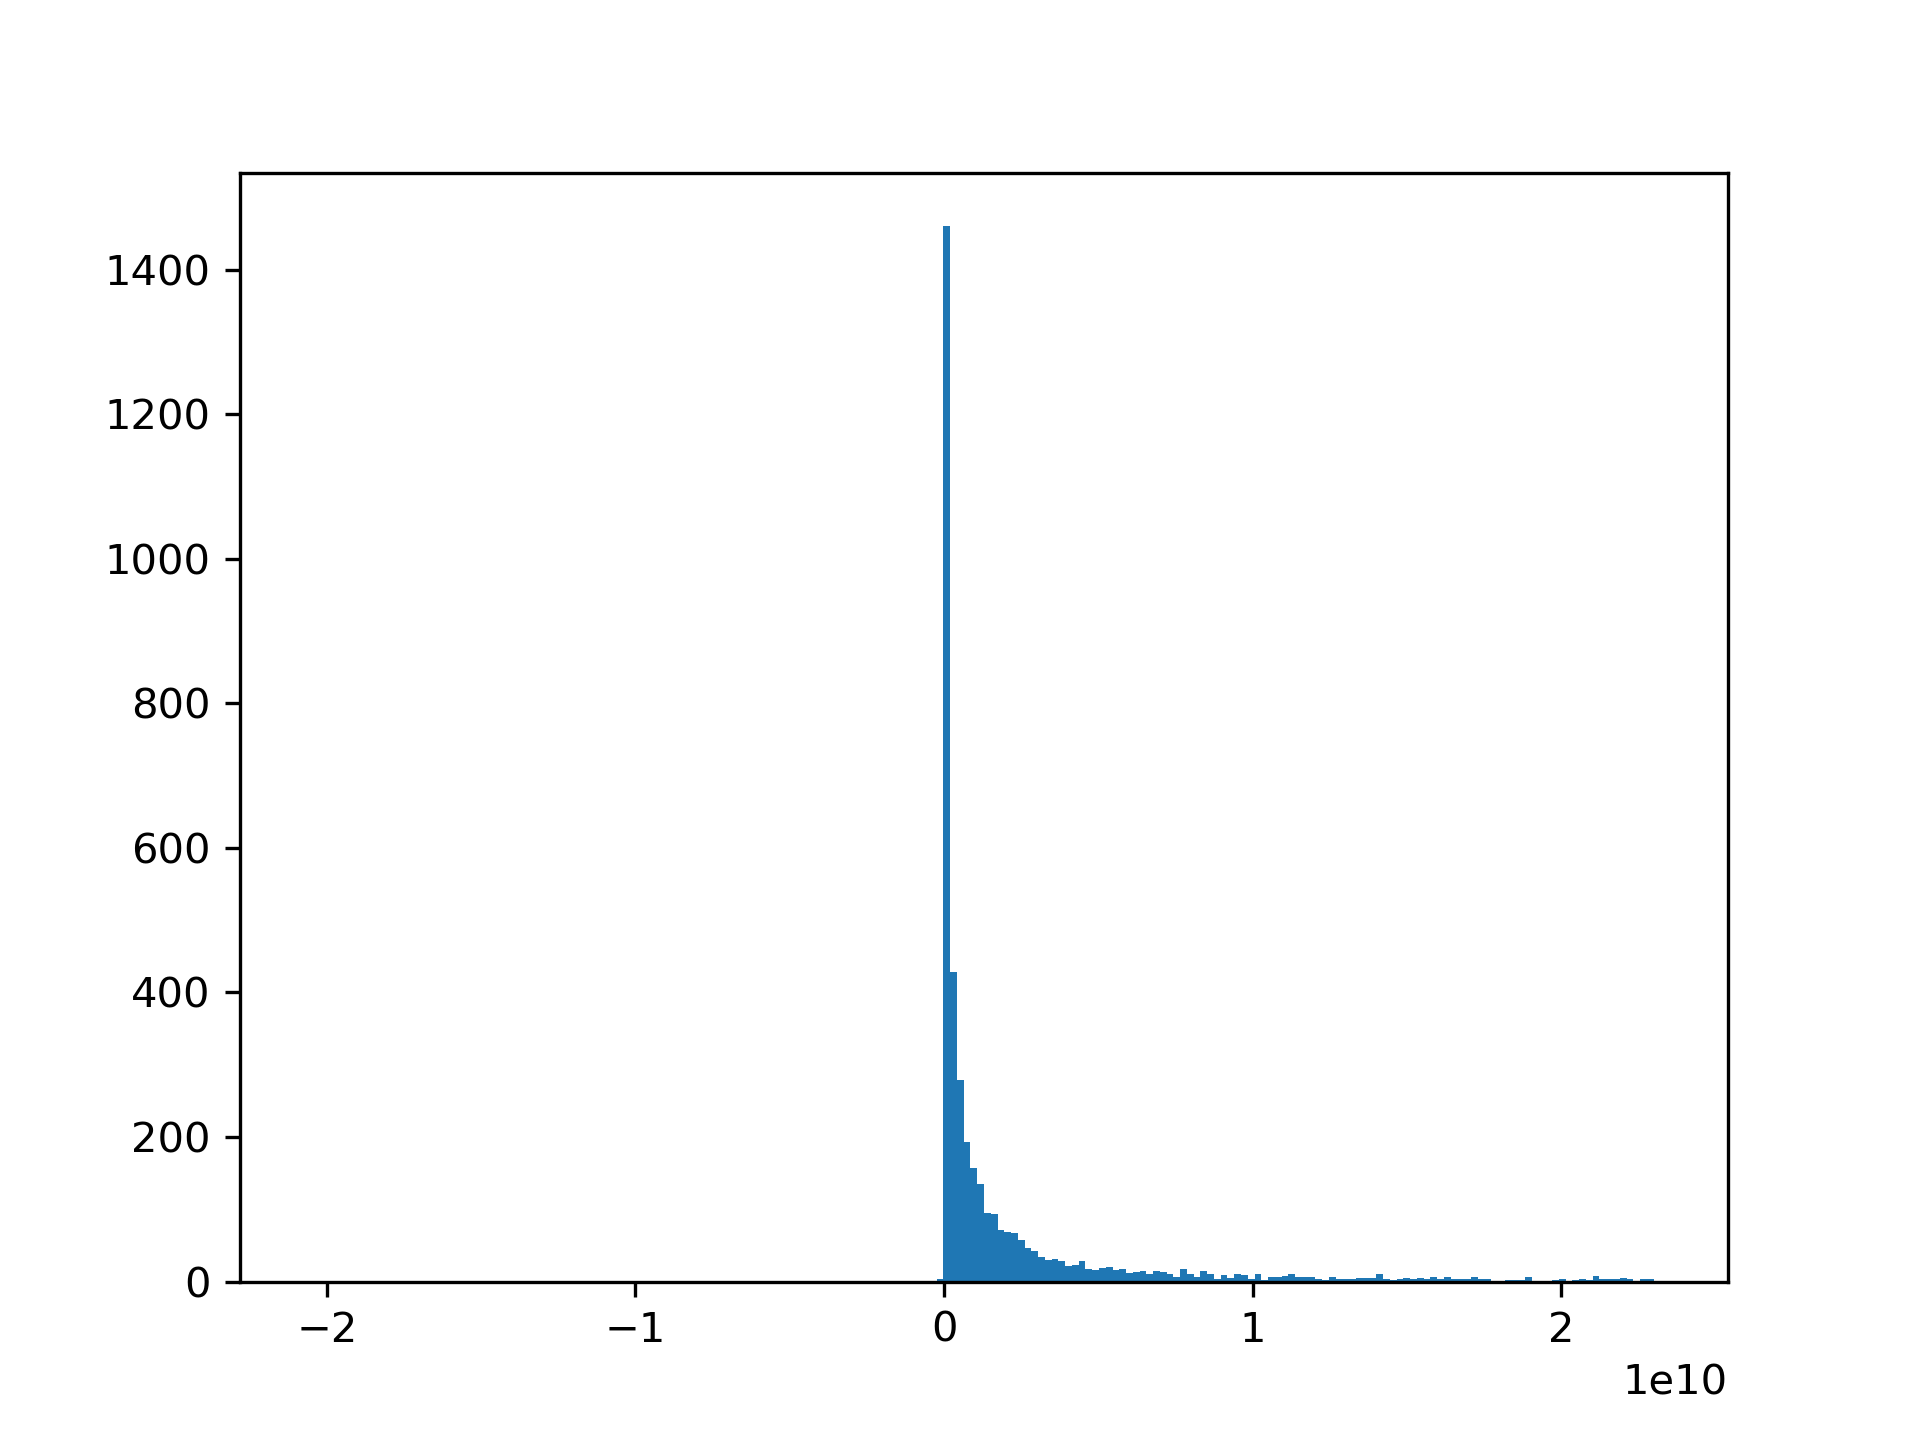
\includegraphics[width=\linewidth]{variables/Revenue.png}
    \caption{Histogram Revenue }
\end{figure}\section{ Revenue Growth }

\begin{center}
    \begin{tabular}{|c | c|} 
    \hline
    Statystyka & Wartość \\
    \hline\hline
    Średnia arytmetyczna & 3.561638411078717 \\ 
    \hline
    Odchylenie standardowe & 198.58701014435525 \\
    \hline
    Kwartyl dolny & 0.0 \\
    \hline
    Mediana & 0.0761 \\
    \hline
    Kwartyl górny & 0.18845 \\
    \hline
    Wartość najmniejsza & -3.4615 \\
    \hline
    Wartość największa & 12739.0 \\
    \hline
   \end{tabular}
\end{center}

\begin{figure}[h!]
    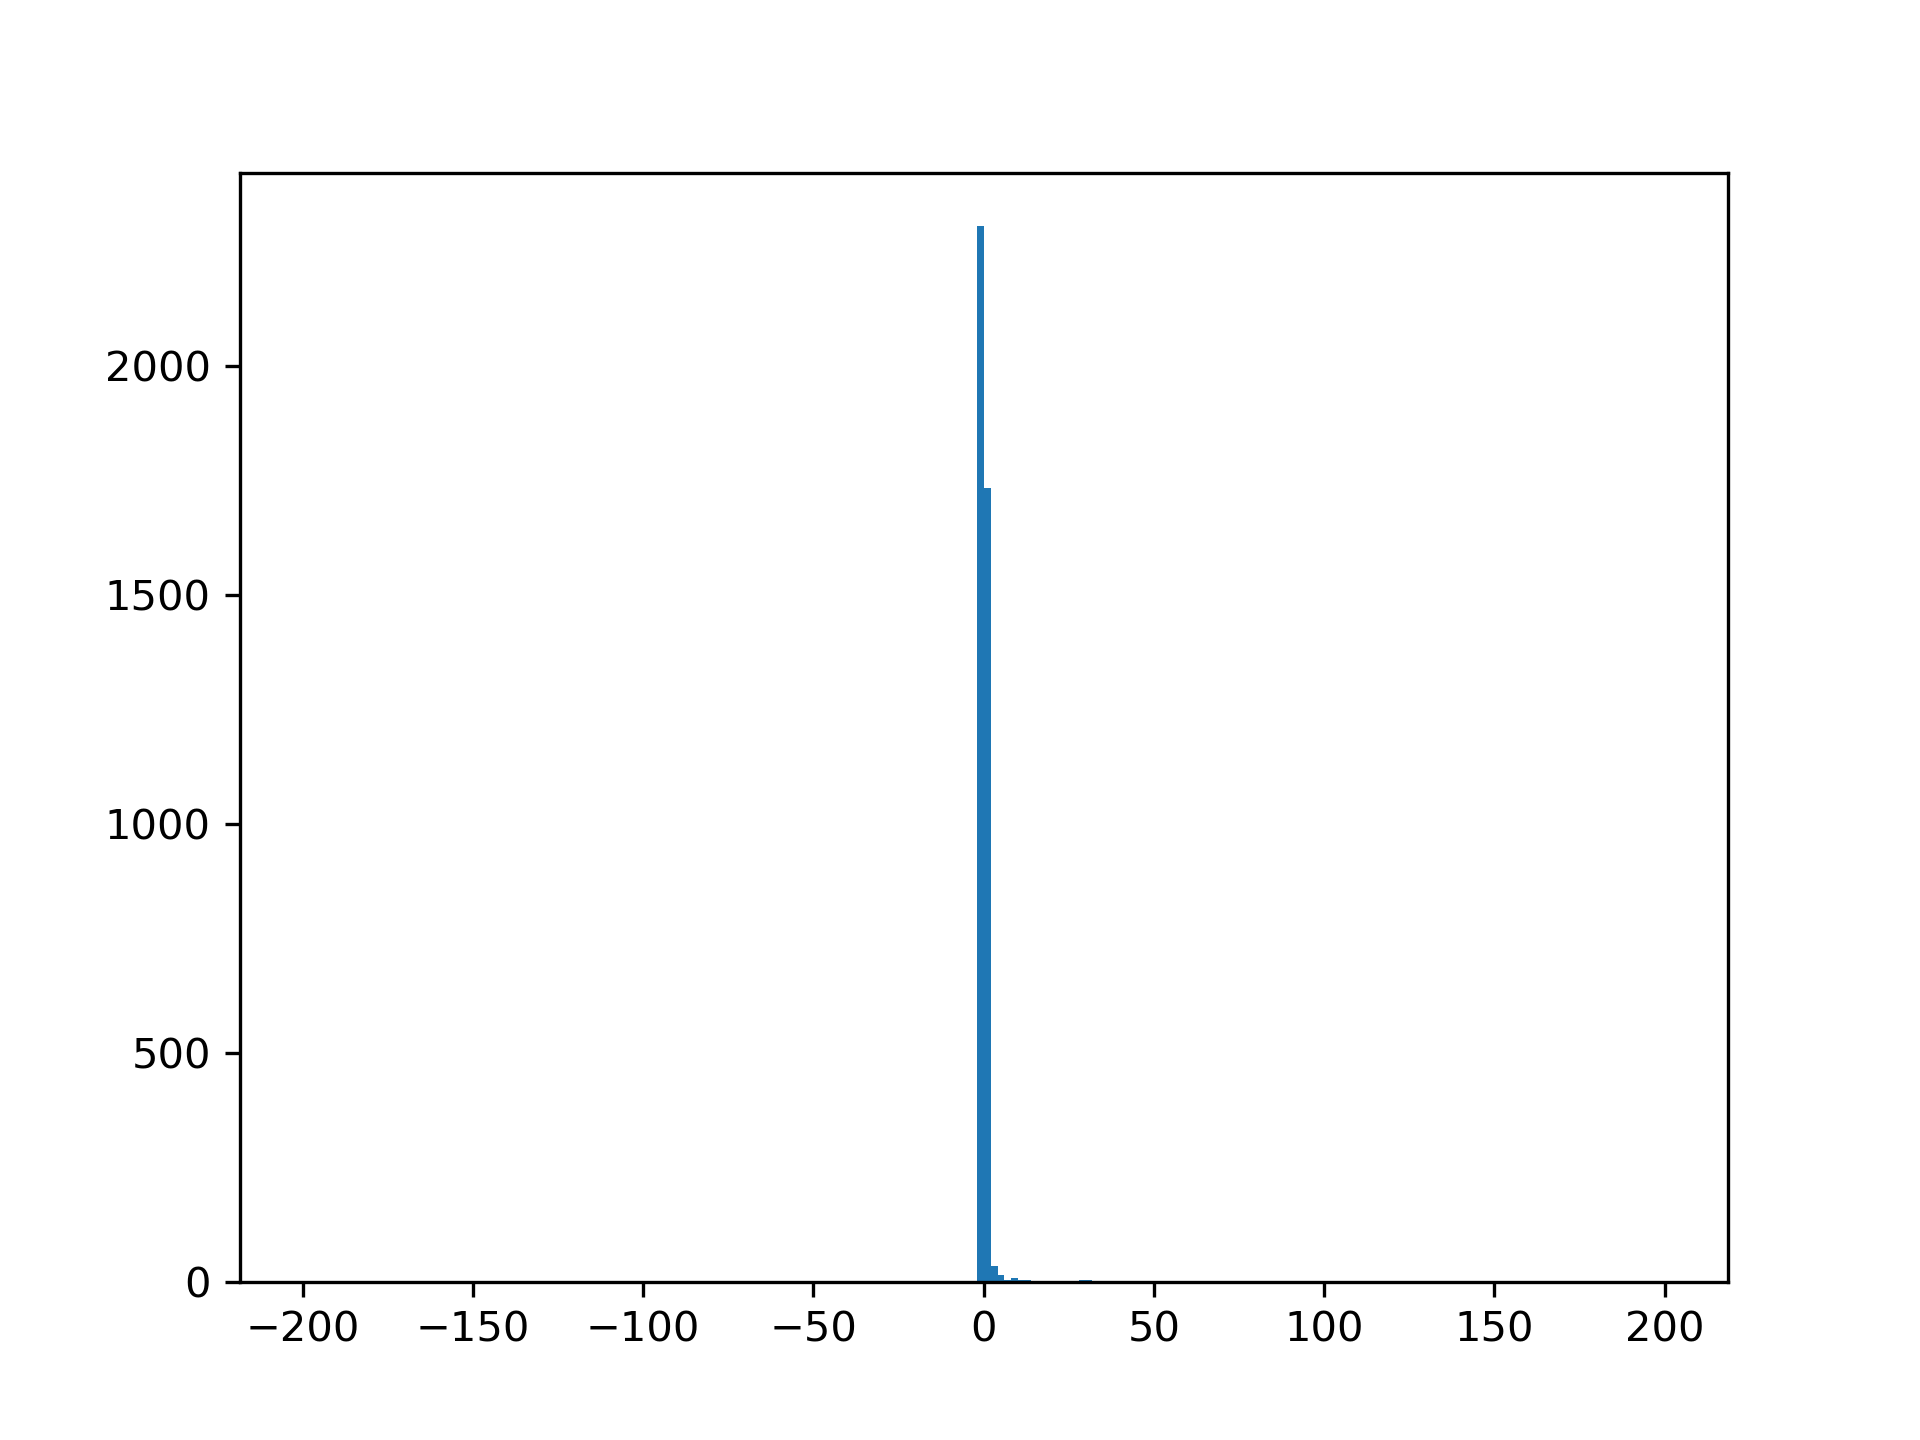
\includegraphics[width=\linewidth]{variables/Revenue Growth.png}
    \caption{Histogram Revenue Growth }
\end{figure}\section{ Cost of Revenue }

\begin{center}
    \begin{tabular}{|c | c|} 
    \hline
    Statystyka & Wartość \\
    \hline\hline
    Średnia arytmetyczna & 3092594116.4171023 \\ 
    \hline
    Odchylenie standardowe & 15146350192.591232 \\
    \hline
    Kwartyl dolny & 3449750.0 \\
    \hline
    Mediana & 172085477.4536 \\
    \hline
    Kwartyl górny & 1269732000.0 \\
    \hline
    Wartość najmniejsza & -2669055283.0189 \\
    \hline
    Wartość największa & 373396000000.0 \\
    \hline
   \end{tabular}
\end{center}

\begin{figure}[h!]
    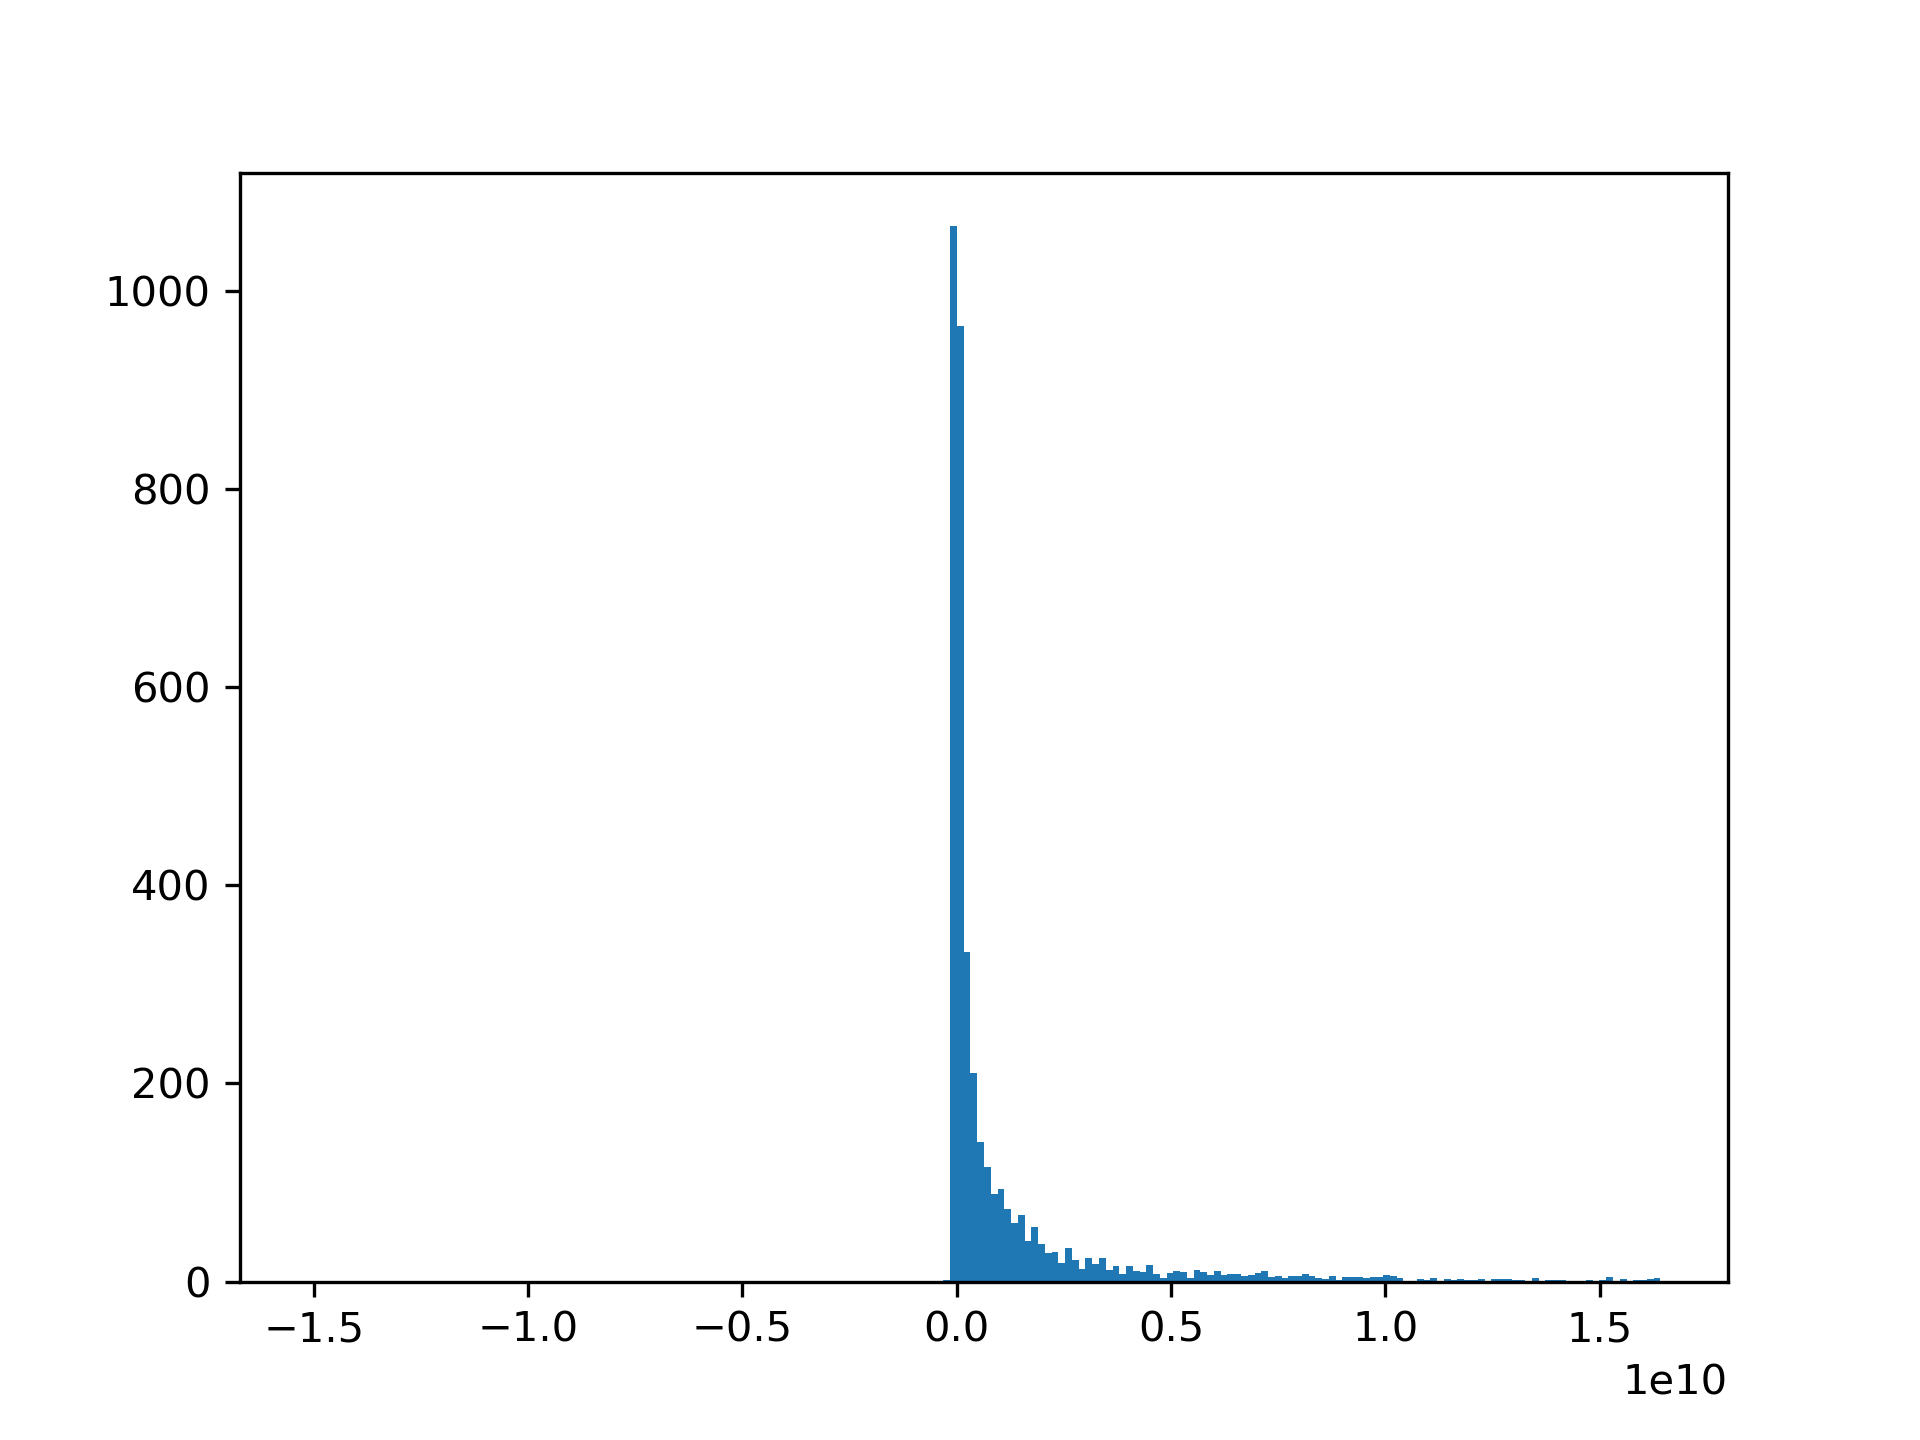
\includegraphics[width=\linewidth]{variables/Cost of Revenue.png}
    \caption{Histogram Cost of Revenue }
\end{figure}\section{ Gross Profit }

\begin{center}
    \begin{tabular}{|c | c|} 
    \hline
    Statystyka & Wartość \\
    \hline\hline
    Średnia arytmetyczna & 2060625005.2207901 \\ 
    \hline
    Odchylenie standardowe & 7664386961.095867 \\
    \hline
    Kwartyl dolny & 39676486.5 \\
    \hline
    Mediana & 243967500.0 \\
    \hline
    Kwartyl górny & 1003508500.0 \\
    \hline
    Wartość najmniejsza & -1818220000.0 \\
    \hline
    Wartość największa & 126947000000.0 \\
    \hline
   \end{tabular}
\end{center}

\begin{figure}[h!]
    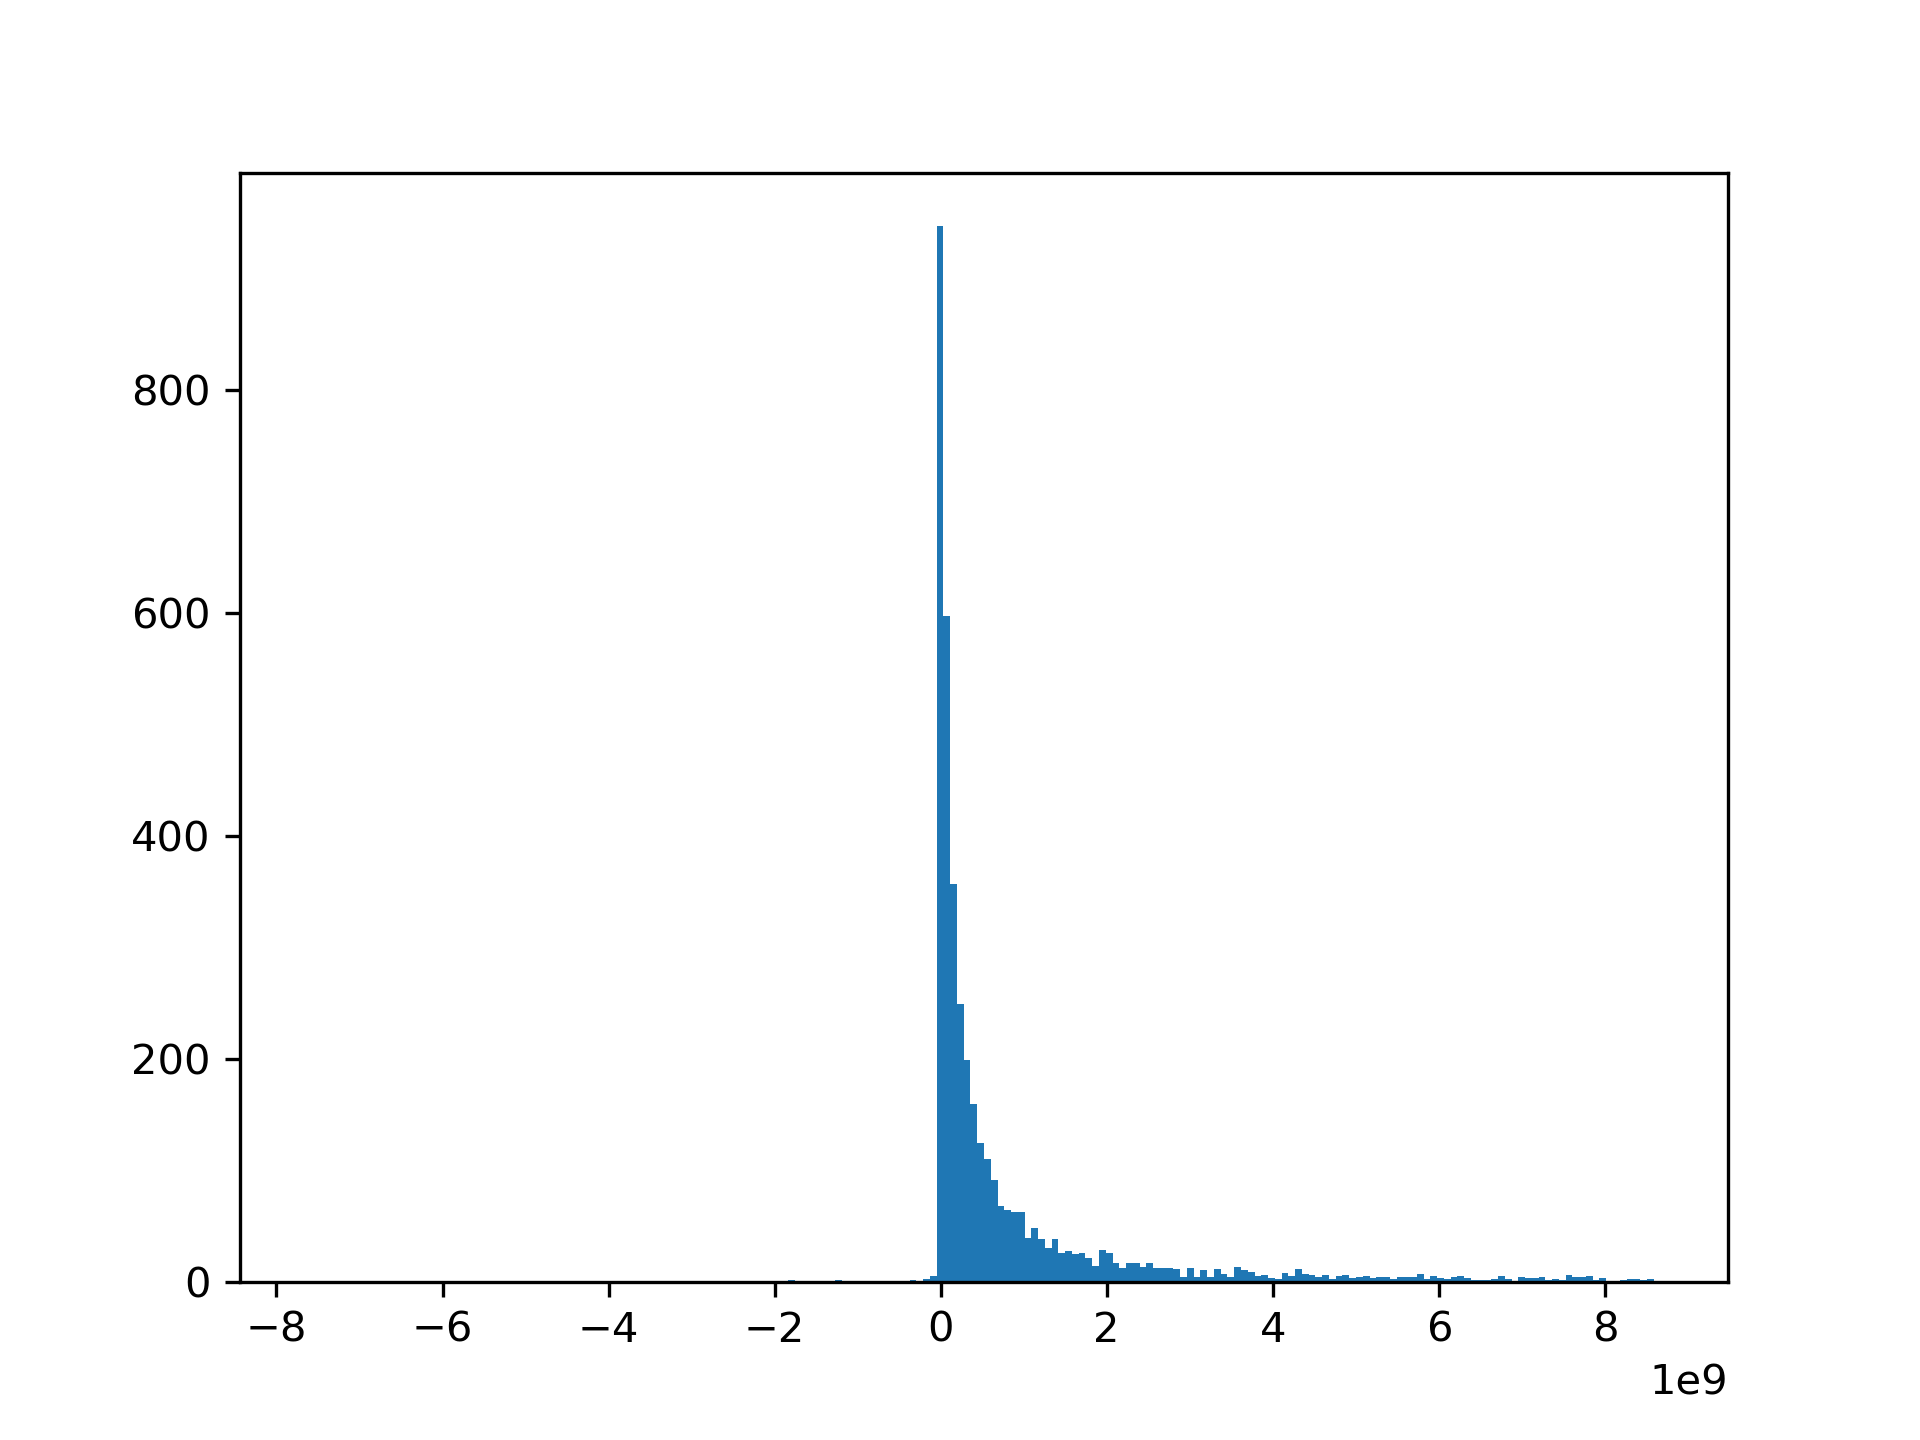
\includegraphics[width=\linewidth]{variables/Gross Profit.png}
    \caption{Histogram Gross Profit }
\end{figure}\section{ RandD Expenses }

\begin{center}
    \begin{tabular}{|c | c|} 
    \hline
    Statystyka & Wartość \\
    \hline\hline
    Średnia arytmetyczna & 113364883.46009417 \\ 
    \hline
    Odchylenie standardowe & 875967333.5123388 \\
    \hline
    Kwartyl dolny & 0.0 \\
    \hline
    Mediana & 0.0 \\
    \hline
    Kwartyl górny & 14463250.0 \\
    \hline
    Wartość najmniejsza & -104200000.0 \\
    \hline
    Wartość największa & 28837000000.0 \\
    \hline
   \end{tabular}
\end{center}

\begin{figure}[h!]
    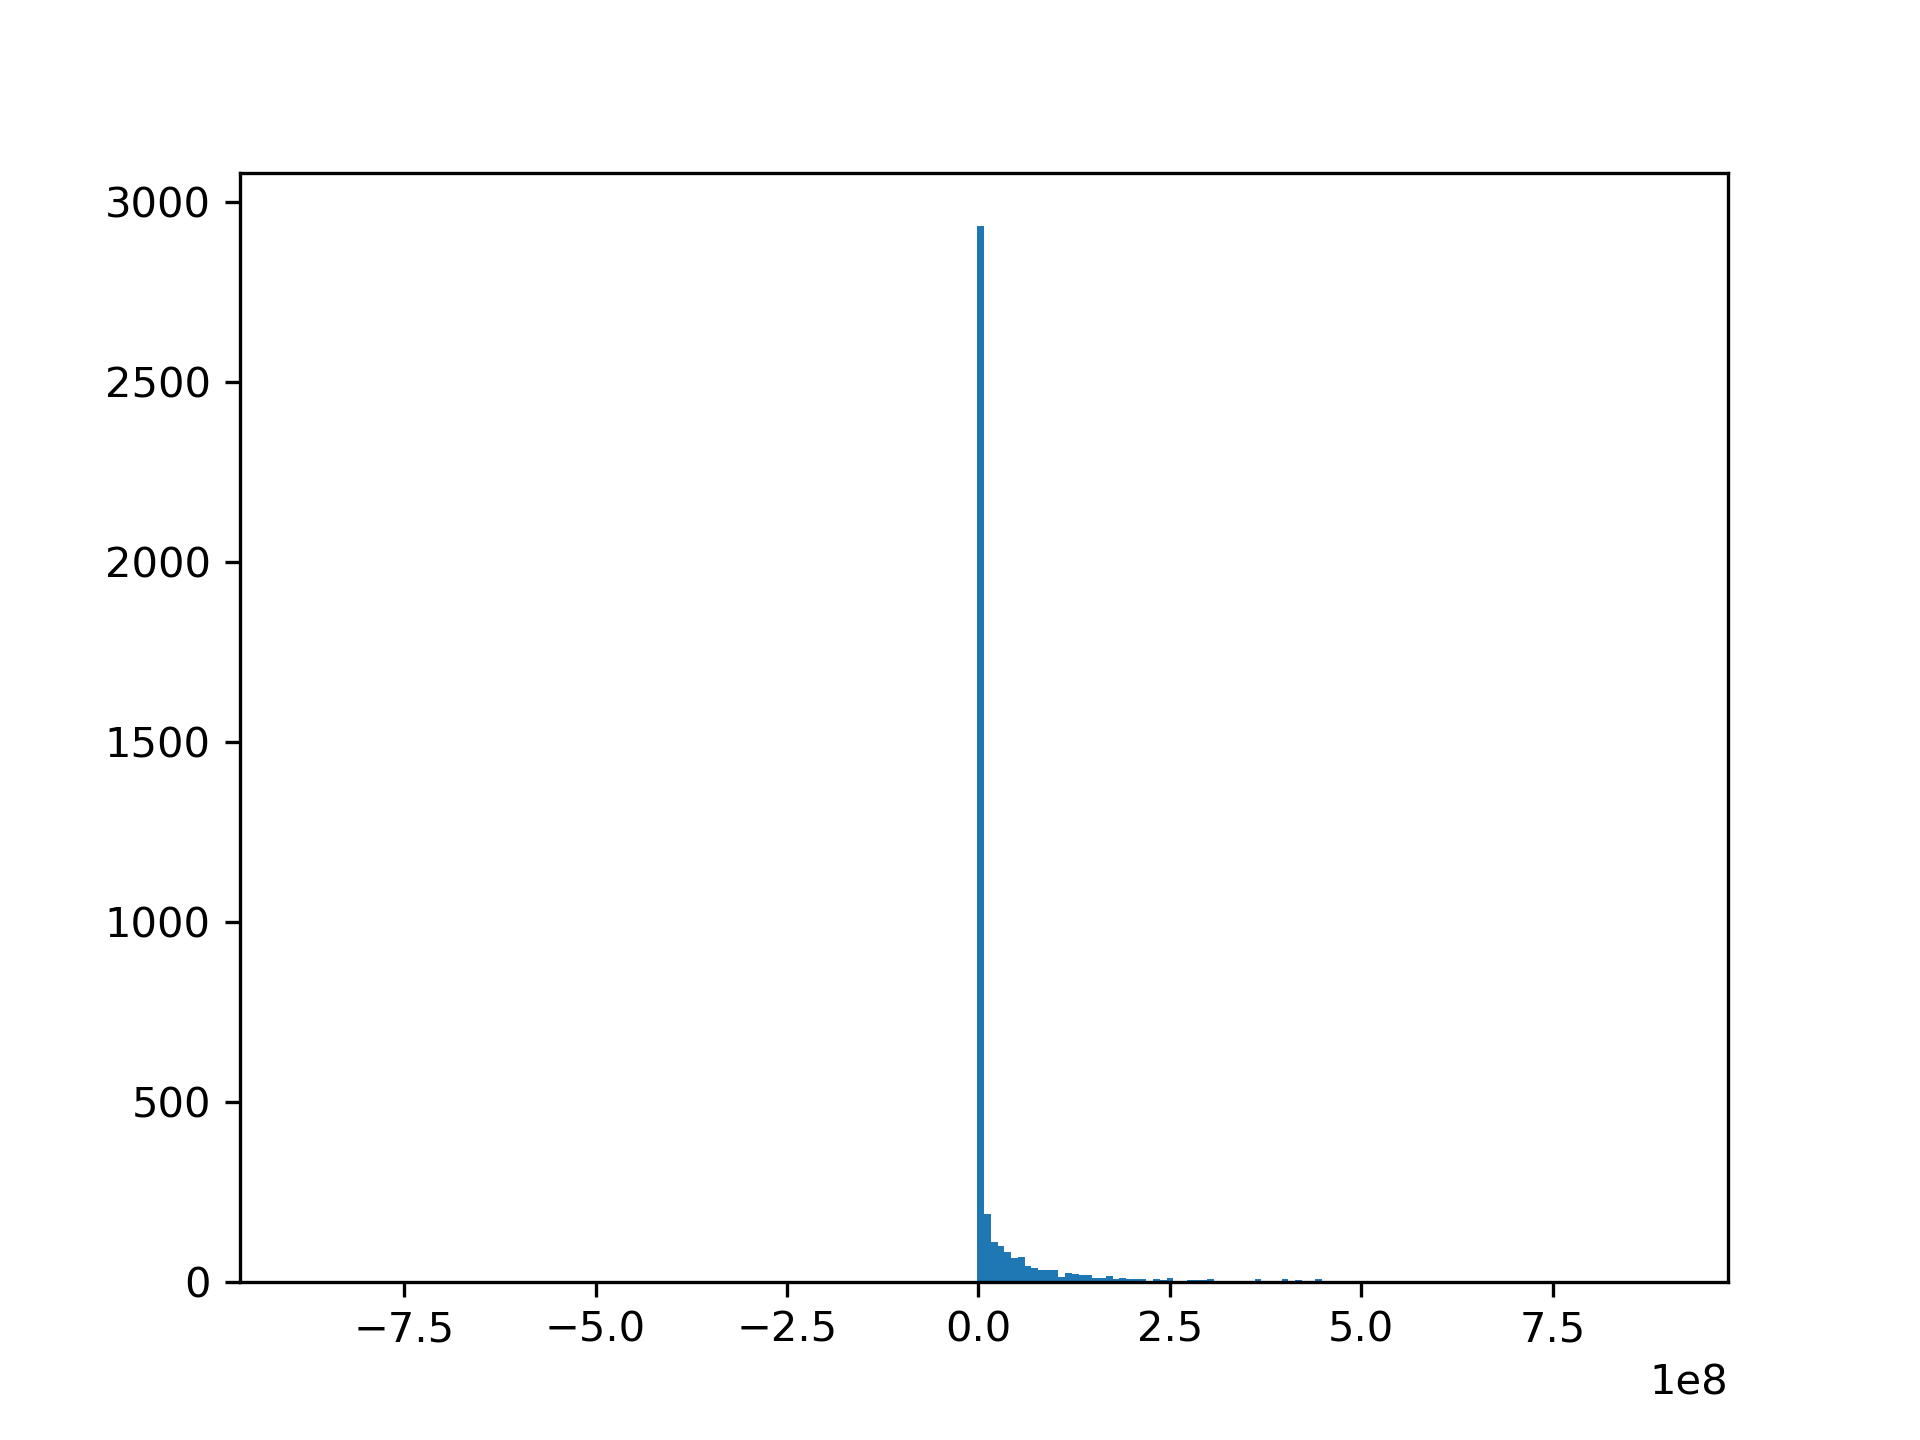
\includegraphics[width=\linewidth]{variables/R_D Expenses.png}
    \caption{Histogram RandD Expenses }
\end{figure}\section{ SGandA Expense }

\begin{center}
    \begin{tabular}{|c | c|} 
    \hline
    Statystyka & Wartość \\
    \hline\hline
    Średnia arytmetyczna & 895678899.924177 \\ 
    \hline
    Odchylenie standardowe & 3651897322.4409237 \\
    \hline
    Kwartyl dolny & 20896500.0 \\
    \hline
    Mediana & 94104500.0 \\
    \hline
    Kwartyl górny & 405750000.0 \\
    \hline
    Wartość najmniejsza & -140159420.2899 \\
    \hline
    Wartość największa & 106510000000.0 \\
    \hline
   \end{tabular}
\end{center}

\begin{figure}[h!]
    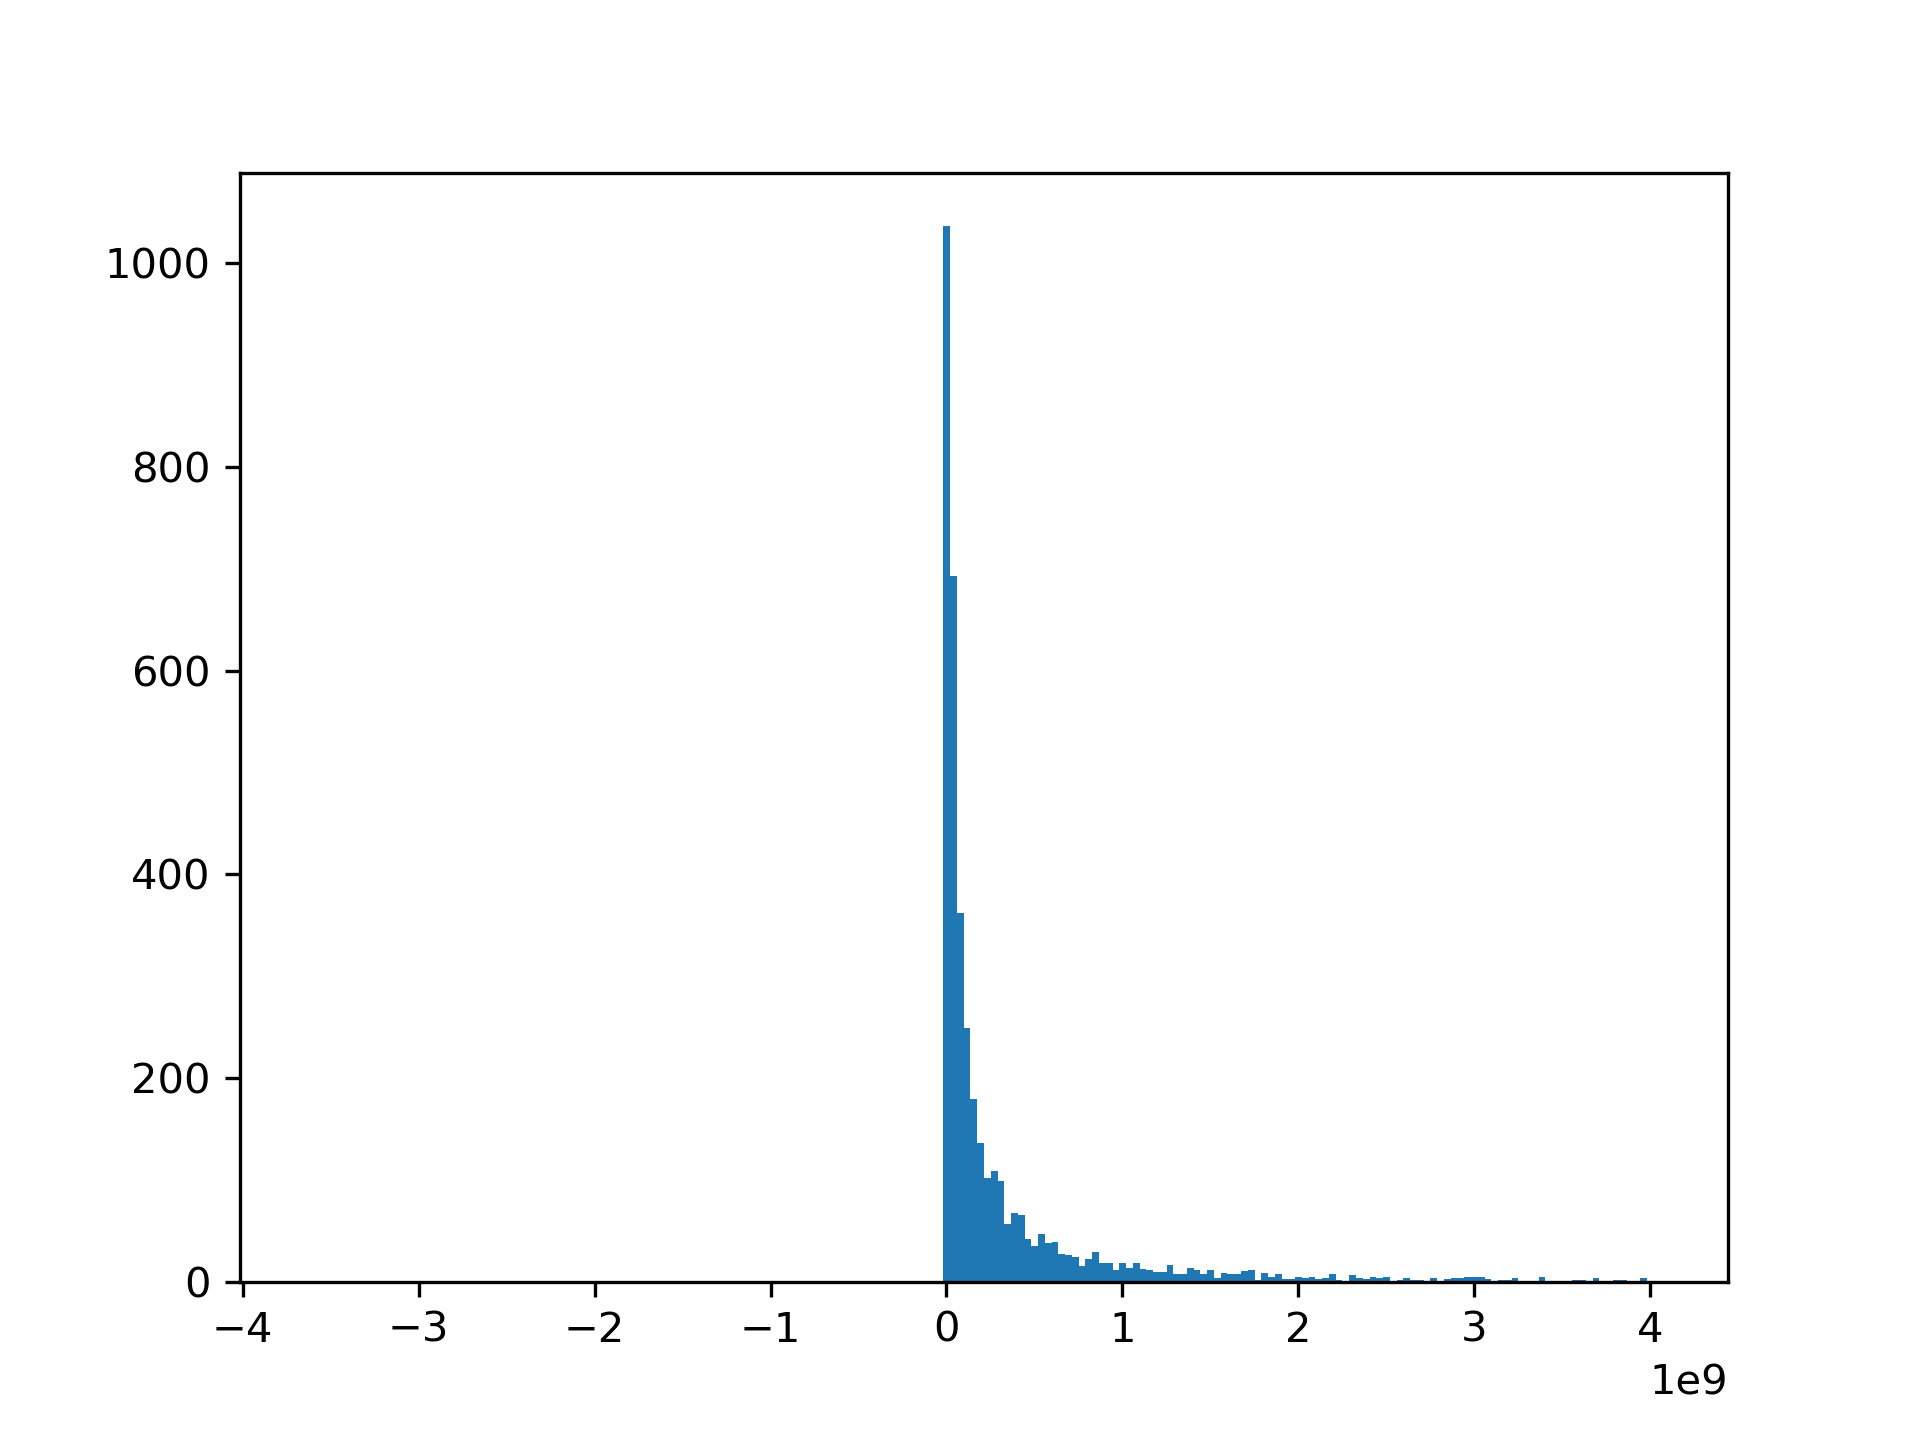
\includegraphics[width=\linewidth]{variables/SG_A Expense.png}
    \caption{Histogram SGandA Expense }
\end{figure}\section{ Operating Expenses }

\begin{center}
    \begin{tabular}{|c | c|} 
    \hline
    Statystyka & Wartość \\
    \hline\hline
    Średnia arytmetyczna & 1415276926.3036318 \\ 
    \hline
    Odchylenie standardowe & 5475134773.371551 \\
    \hline
    Kwartyl dolny & 43734500.0 \\
    \hline
    Mediana & 182541572.5 \\
    \hline
    Kwartyl górny & 677066172.6804 \\
    \hline
    Wartość najmniejsza & -4280000000.0 \\
    \hline
    Wartość największa & 106510000000.0 \\
    \hline
   \end{tabular}
\end{center}

\begin{figure}[h!]
    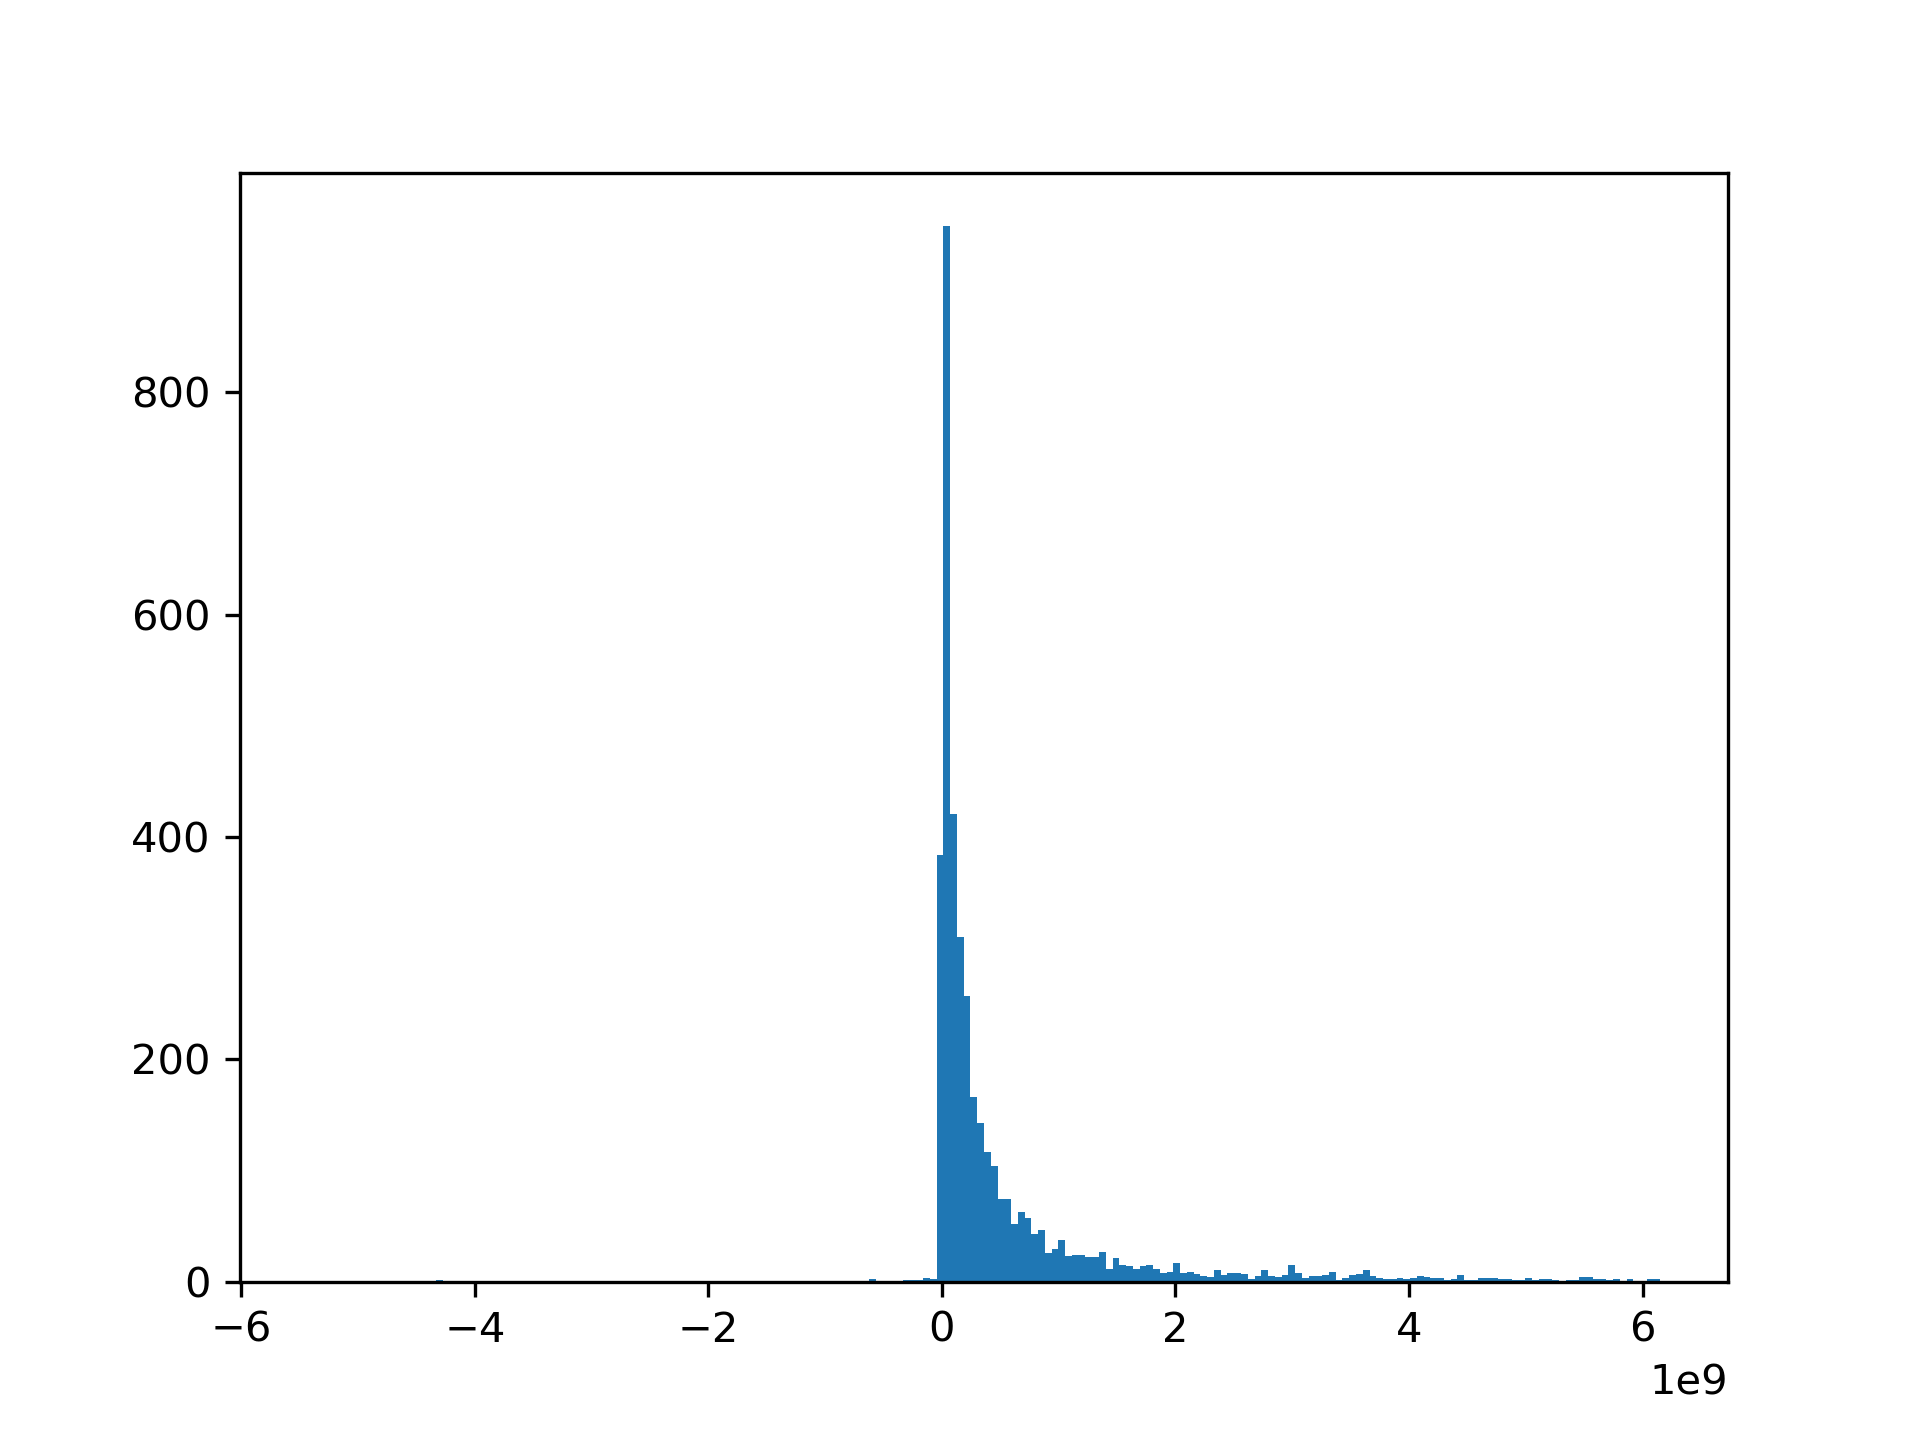
\includegraphics[width=\linewidth]{variables/Operating Expenses.png}
    \caption{Histogram Operating Expenses }
\end{figure}\section{ Operating Income }

\begin{center}
    \begin{tabular}{|c | c|} 
    \hline
    Statystyka & Wartość \\
    \hline\hline
    Średnia arytmetyczna & 645248675.4661082 \\ 
    \hline
    Odchylenie standardowe & 2947874412.4589252 \\
    \hline
    Kwartyl dolny & -5348678.25 \\
    \hline
    Mediana & 46110500.0 \\
    \hline
    Kwartyl górny & 293183000.0 \\
    \hline
    Wartość najmniejsza & -14557000000.0 \\
    \hline
    Wartość największa & 70898000000.0 \\
    \hline
   \end{tabular}
\end{center}

\begin{figure}[h!]
    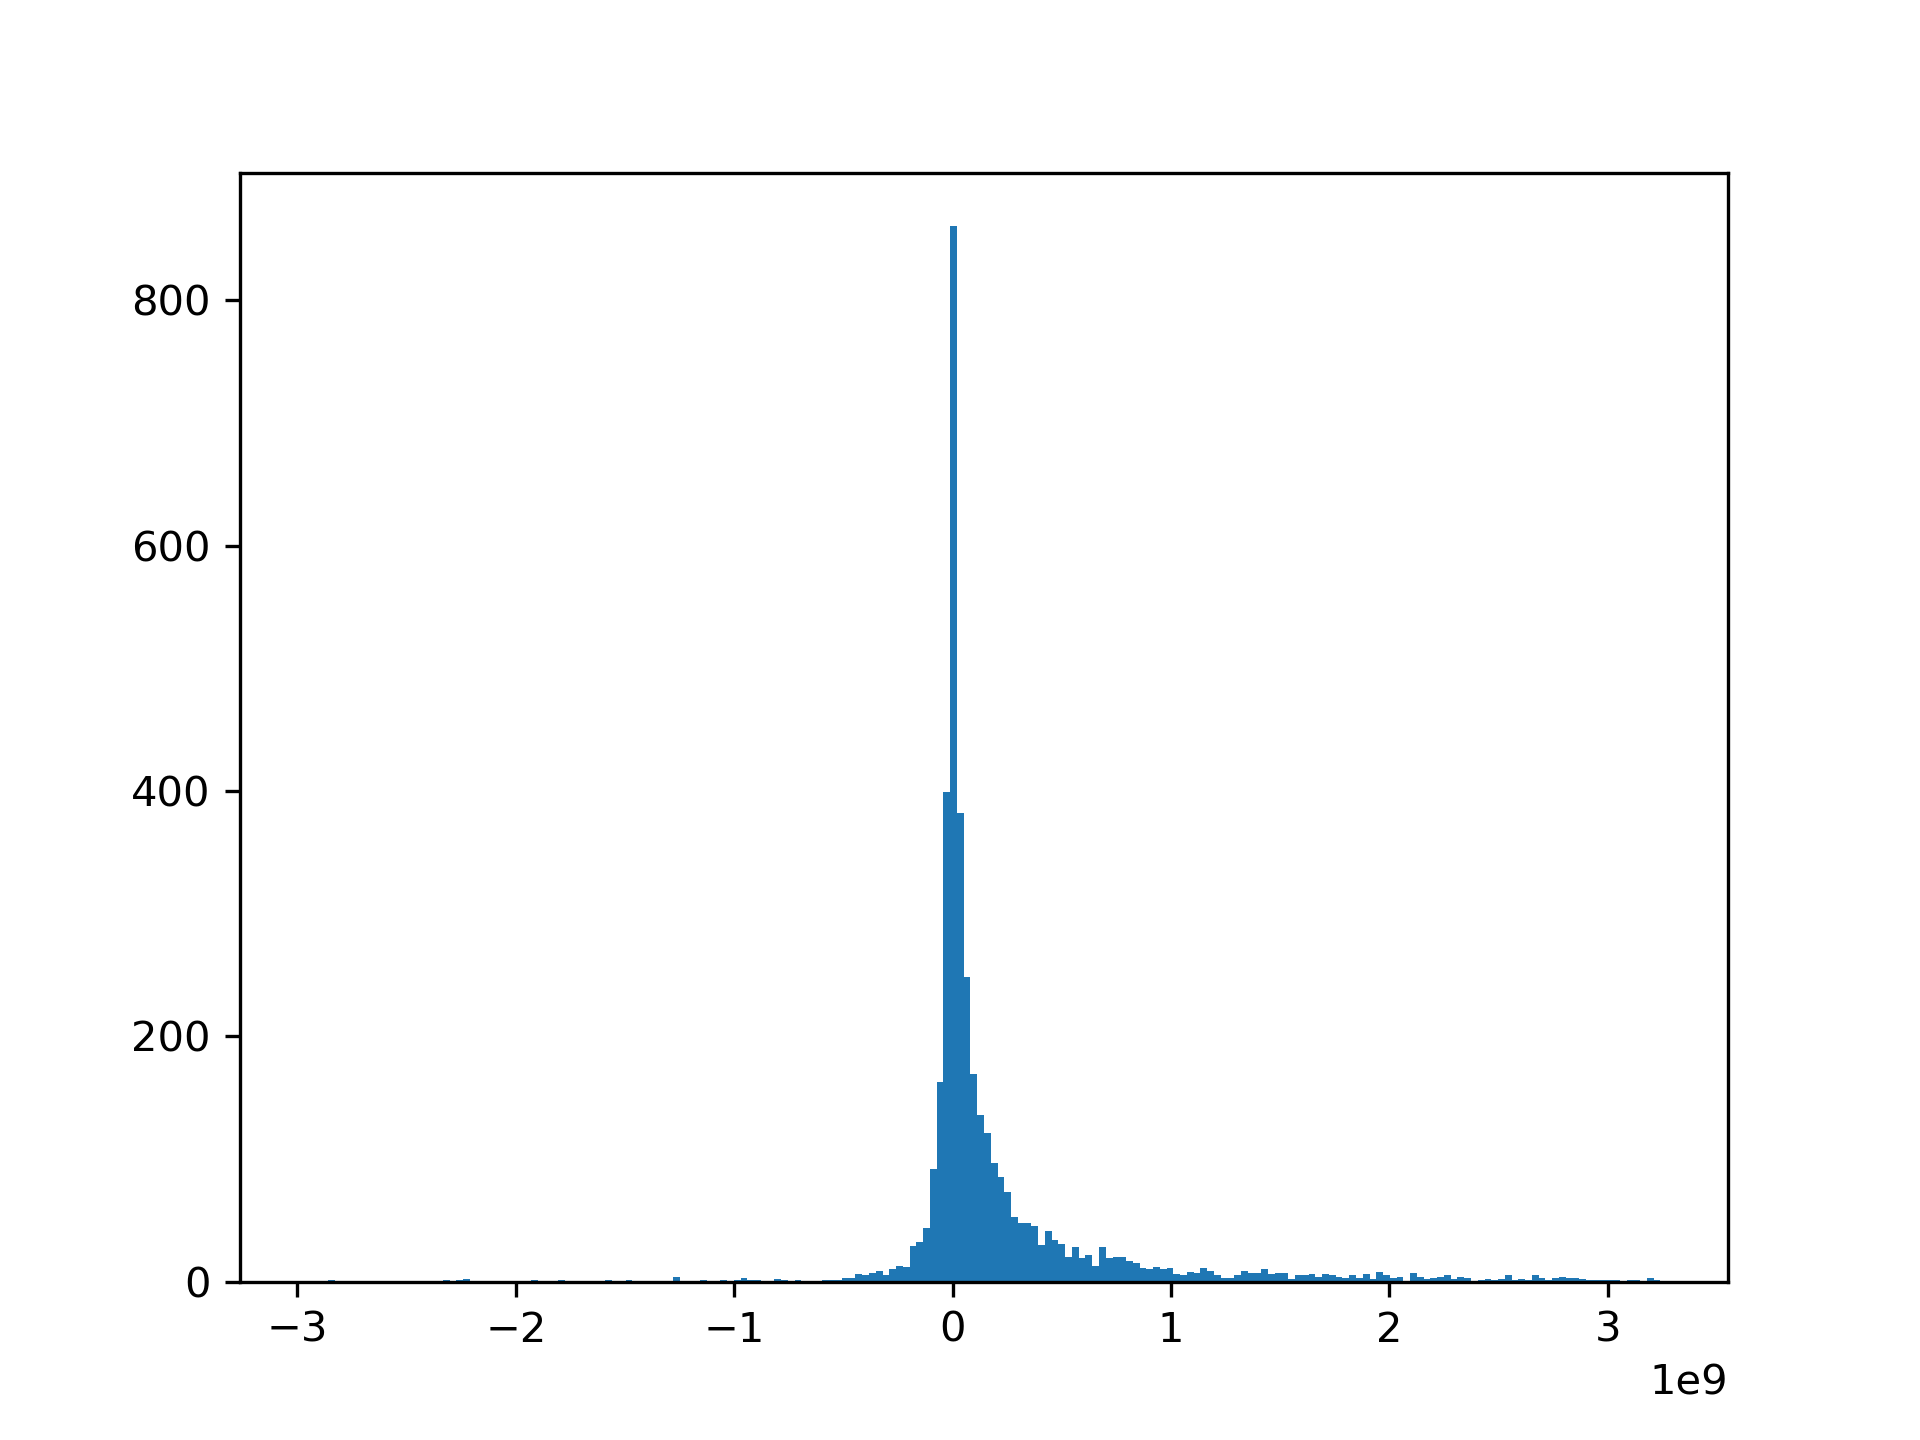
\includegraphics[width=\linewidth]{variables/Operating Income.png}
    \caption{Histogram Operating Income }
\end{figure}\section{ Interest Expense }

\begin{center}
    \begin{tabular}{|c | c|} 
    \hline
    Statystyka & Wartość \\
    \hline\hline
    Średnia arytmetyczna & 98380094.35249001 \\ 
    \hline
    Odchylenie standardowe & 369821186.2794848 \\
    \hline
    Kwartyl dolny & 0.0 \\
    \hline
    Mediana & 5569402.29885 \\
    \hline
    Kwartyl górny & 57311750.0 \\
    \hline
    Wartość najmniejsza & -509503091.3671 \\
    \hline
    Wartość największa & 9168000000.0 \\
    \hline
   \end{tabular}
\end{center}

\begin{figure}[h!]
    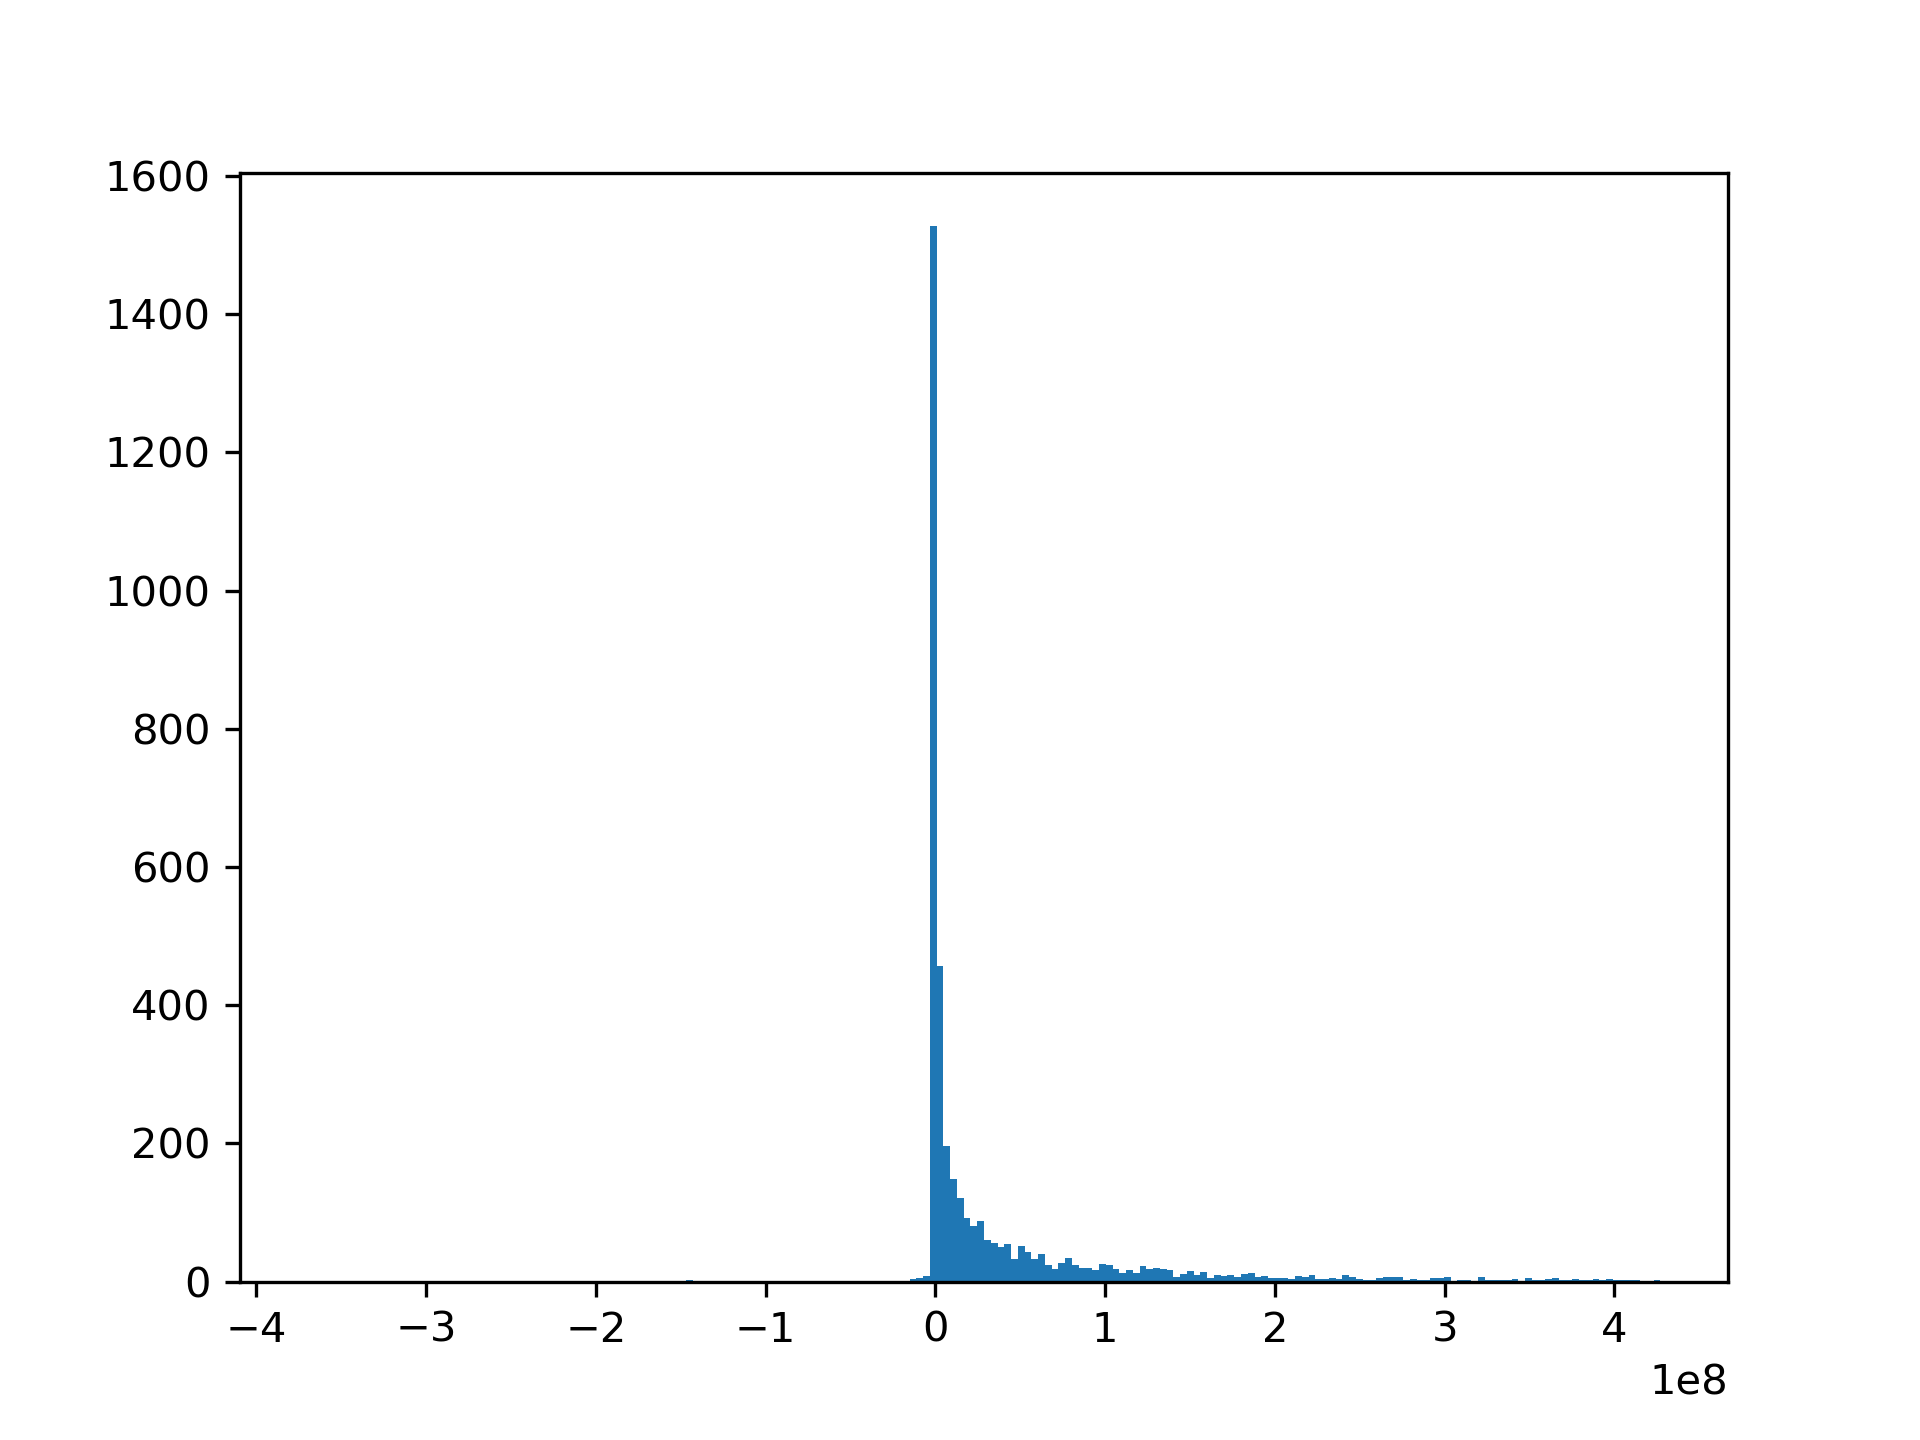
\includegraphics[width=\linewidth]{variables/Interest Expense.png}
    \caption{Histogram Interest Expense }
\end{figure}\section{ Earnings before Tax }

\begin{center}
    \begin{tabular}{|c | c|} 
    \hline
    Statystyka & Wartość \\
    \hline\hline
    Średnia arytmetyczna & 557759742.8667502 \\ 
    \hline
    Odchylenie standardowe & 2614660258.729711 \\
    \hline
    Kwartyl dolny & -9807862.0 \\
    \hline
    Mediana & 30528500.0 \\
    \hline
    Kwartyl górny & 231983250.0 \\
    \hline
    Wartość najmniejsza & -21772000000.0 \\
    \hline
    Wartość największa & 72903000000.0 \\
    \hline
   \end{tabular}
\end{center}

\begin{figure}[h!]
    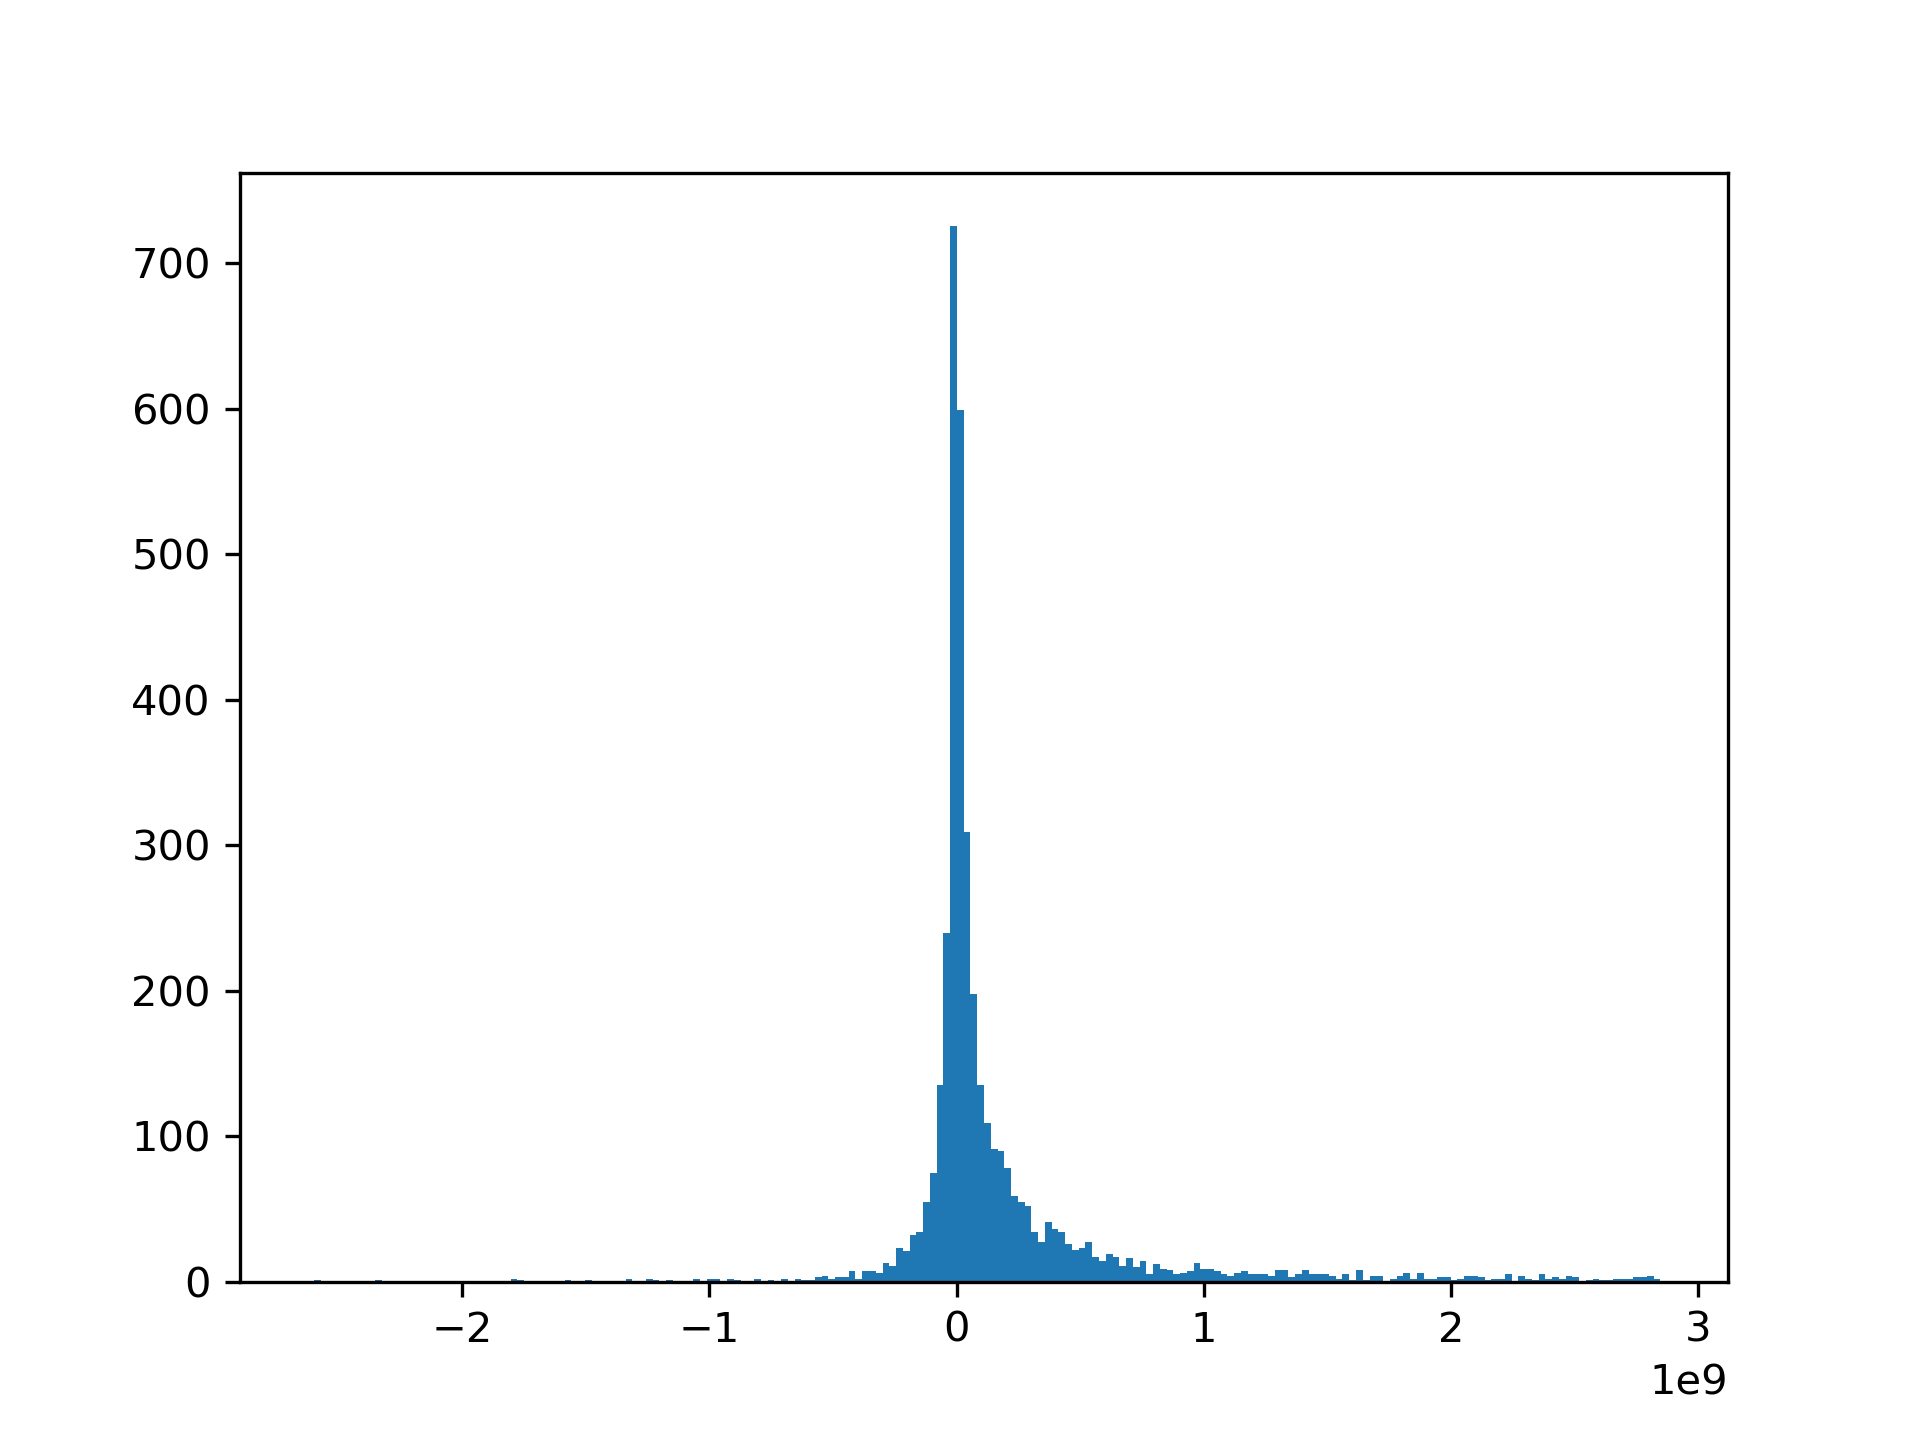
\includegraphics[width=\linewidth]{variables/Earnings before Tax.png}
    \caption{Histogram Earnings before Tax }
\end{figure}\section{ Income Tax Expense }

\begin{center}
    \begin{tabular}{|c | c|} 
    \hline
    Statystyka & Wartość \\
    \hline\hline
    Średnia arytmetyczna & 121371377.72096992 \\ 
    \hline
    Odchylenie standardowe & 725443941.3266019 \\
    \hline
    Kwartyl dolny & 0.0 \\
    \hline
    Mediana & 2780000.0 \\
    \hline
    Kwartyl górny & 40319000.0 \\
    \hline
    Wartość najmniejsza & -8084000000.0 \\
    \hline
    Wartość największa & 19903000000.0 \\
    \hline
   \end{tabular}
\end{center}

\begin{figure}[h!]
    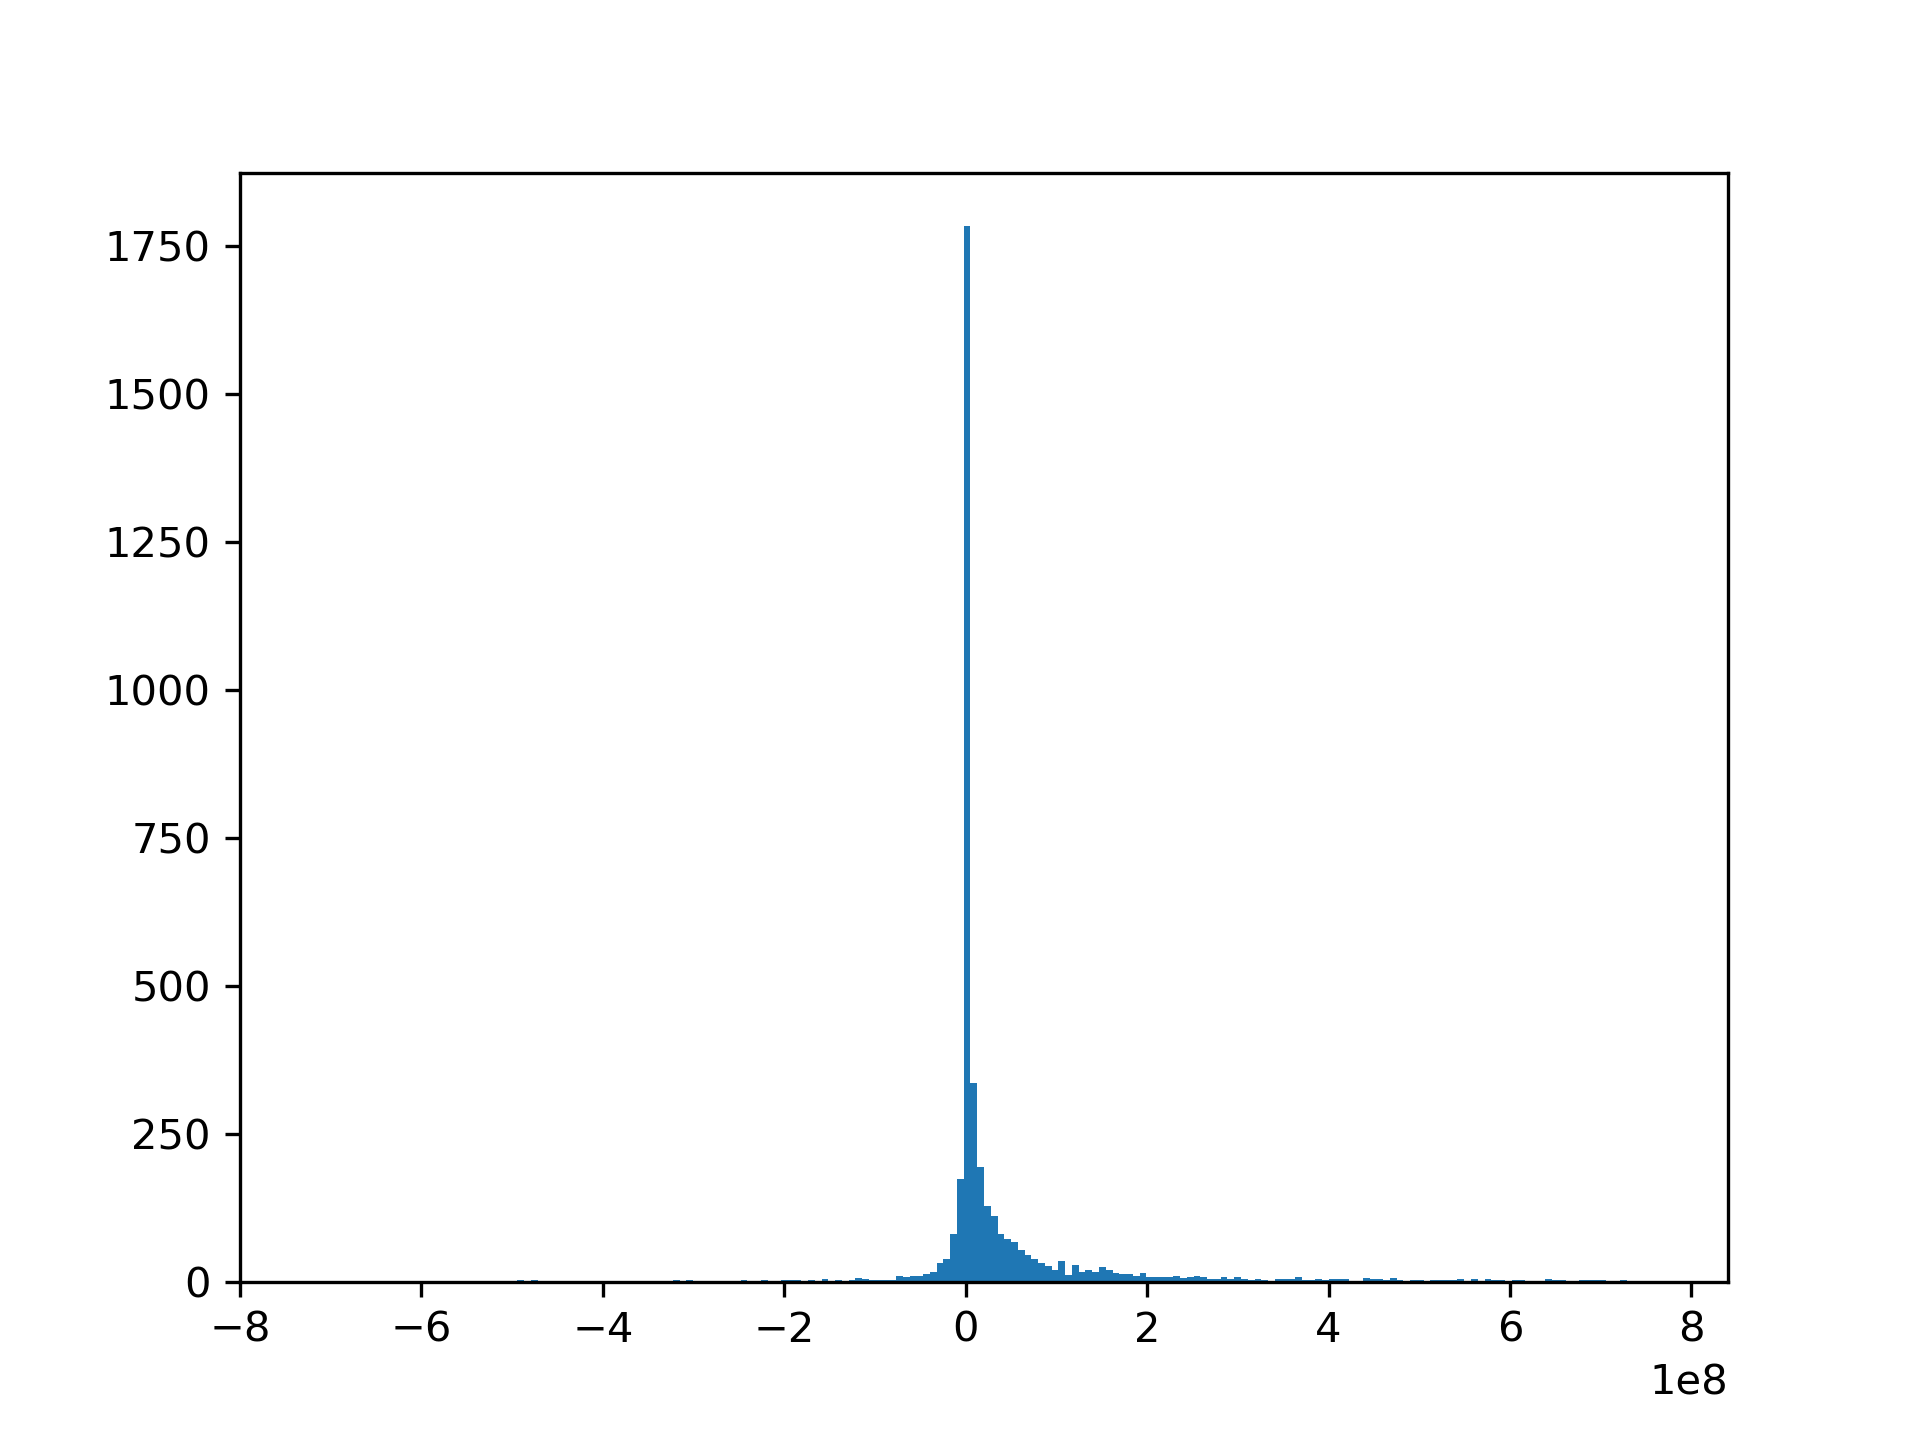
\includegraphics[width=\linewidth]{variables/Income Tax Expense.png}
    \caption{Histogram Income Tax Expense }
\end{figure}\section{ Net Income - Non-Controlling int }

\begin{center}
    \begin{tabular}{|c | c|} 
    \hline
    Statystyka & Wartość \\
    \hline\hline
    Średnia arytmetyczna & 15210992.964401068 \\ 
    \hline
    Odchylenie standardowe & 154217439.24123943 \\
    \hline
    Kwartyl dolny & 0.0 \\
    \hline
    Mediana & 0.0 \\
    \hline
    Kwartyl górny & 0.0 \\
    \hline
    Wartość najmniejsza & -1241116751.269 \\
    \hline
    Wartość największa & 6073227206.9465 \\
    \hline
   \end{tabular}
\end{center}

\begin{figure}[h!]
    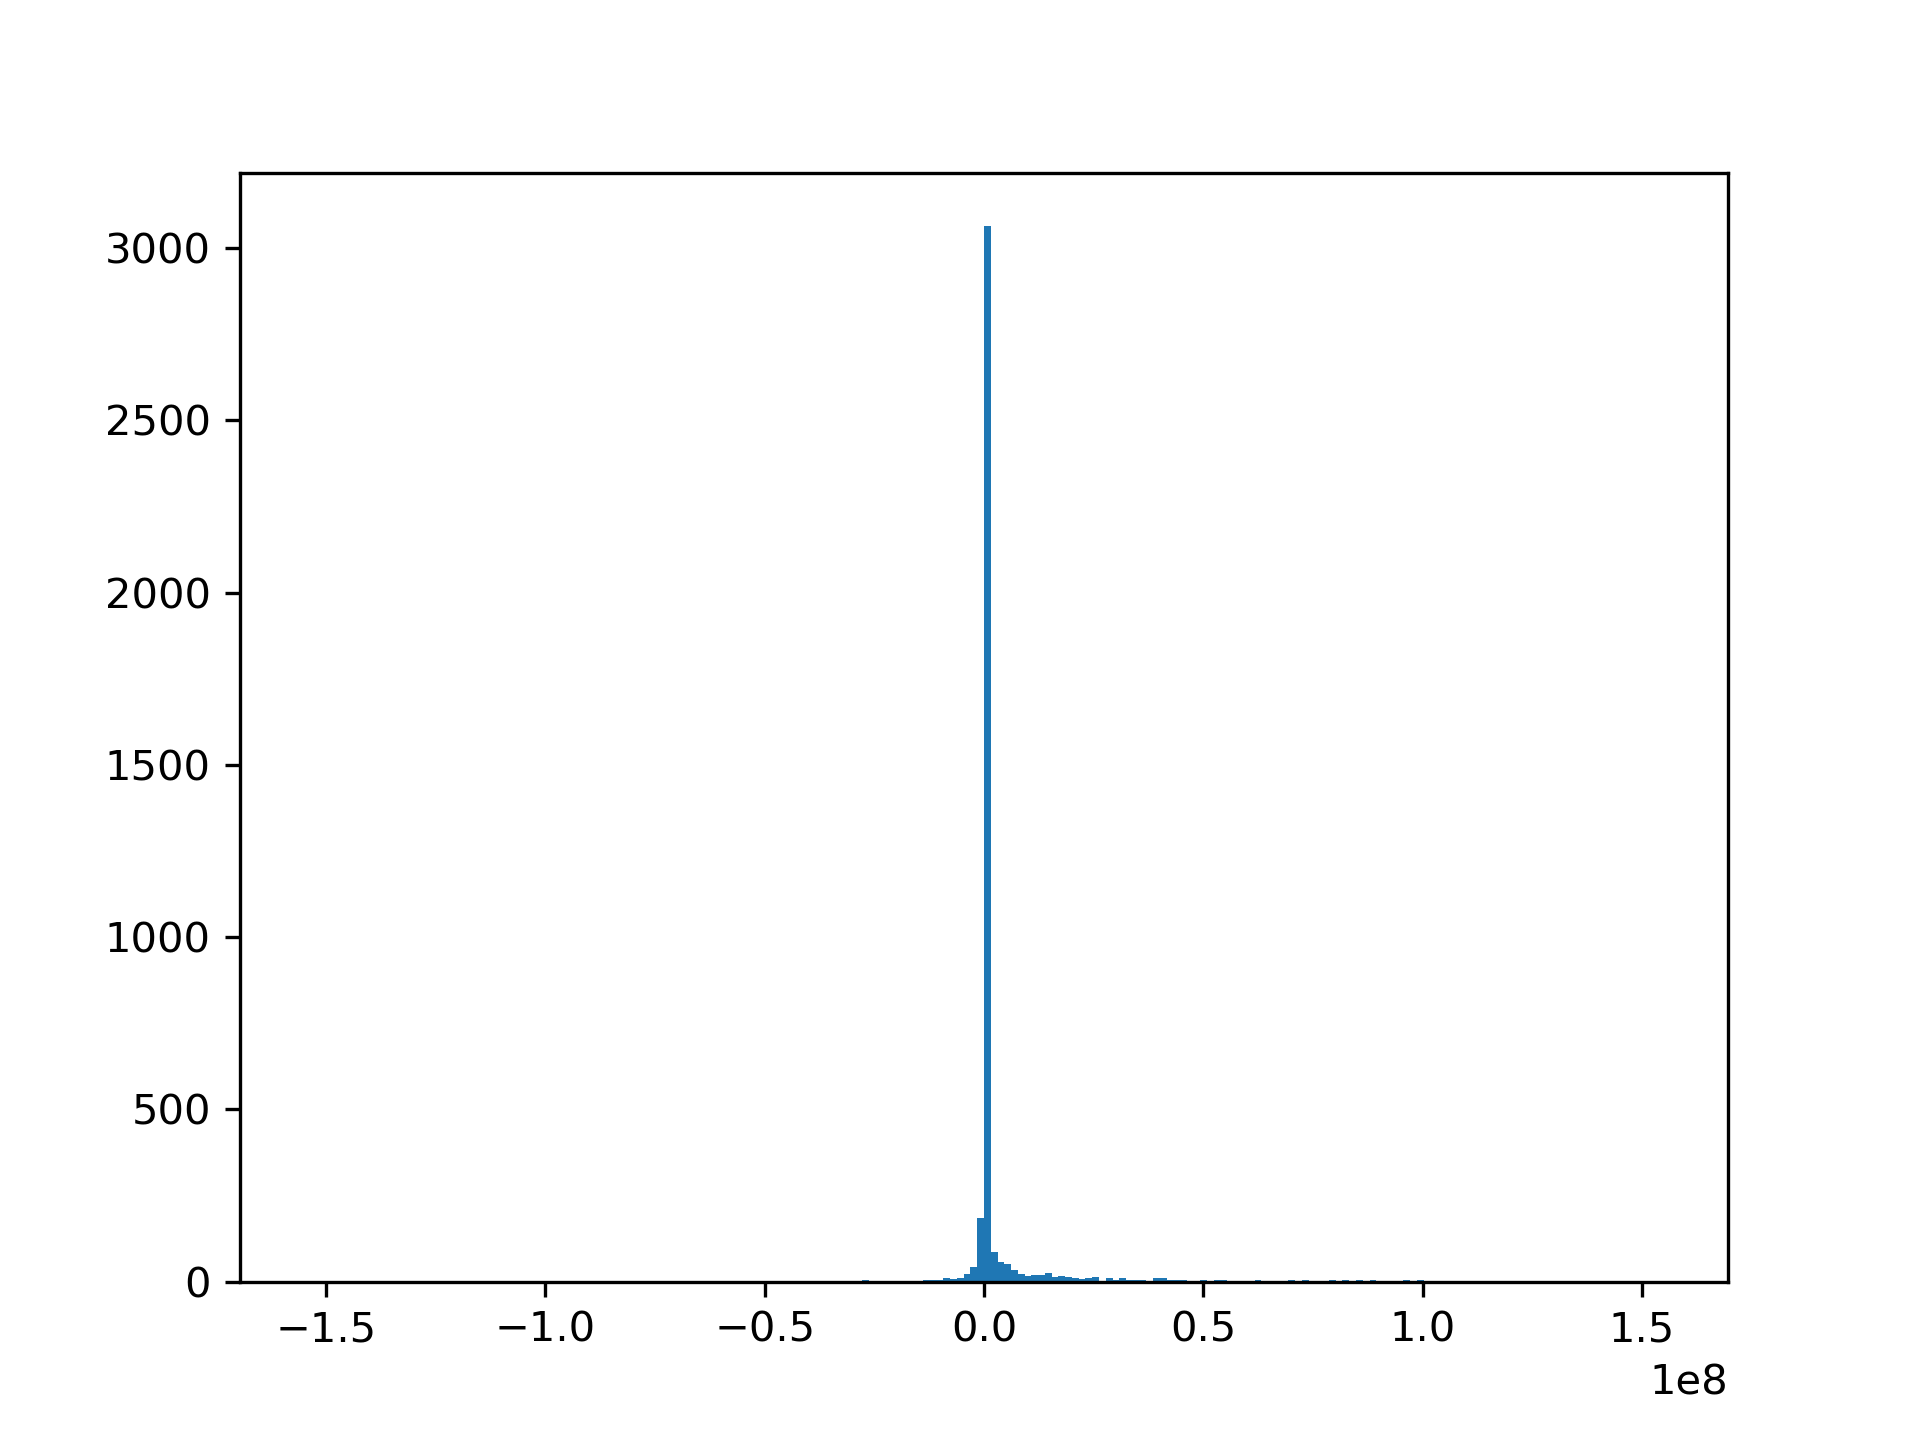
\includegraphics[width=\linewidth]{variables/Net Income - Non-Controlling int.png}
    \caption{Histogram Net Income - Non-Controlling int }
\end{figure}\section{ Net Income - Discontinued ops }

\begin{center}
    \begin{tabular}{|c | c|} 
    \hline
    Statystyka & Wartość \\
    \hline\hline
    Średnia arytmetyczna & -3024333.240941218 \\ 
    \hline
    Odchylenie standardowe & 131894618.98269624 \\
    \hline
    Kwartyl dolny & 0.0 \\
    \hline
    Mediana & 0.0 \\
    \hline
    Kwartyl górny & 0.0 \\
    \hline
    Wartość najmniejsza & -3859000000.0 \\
    \hline
    Wartość największa & 2921000000.0 \\
    \hline
   \end{tabular}
\end{center}

\begin{figure}[h!]
    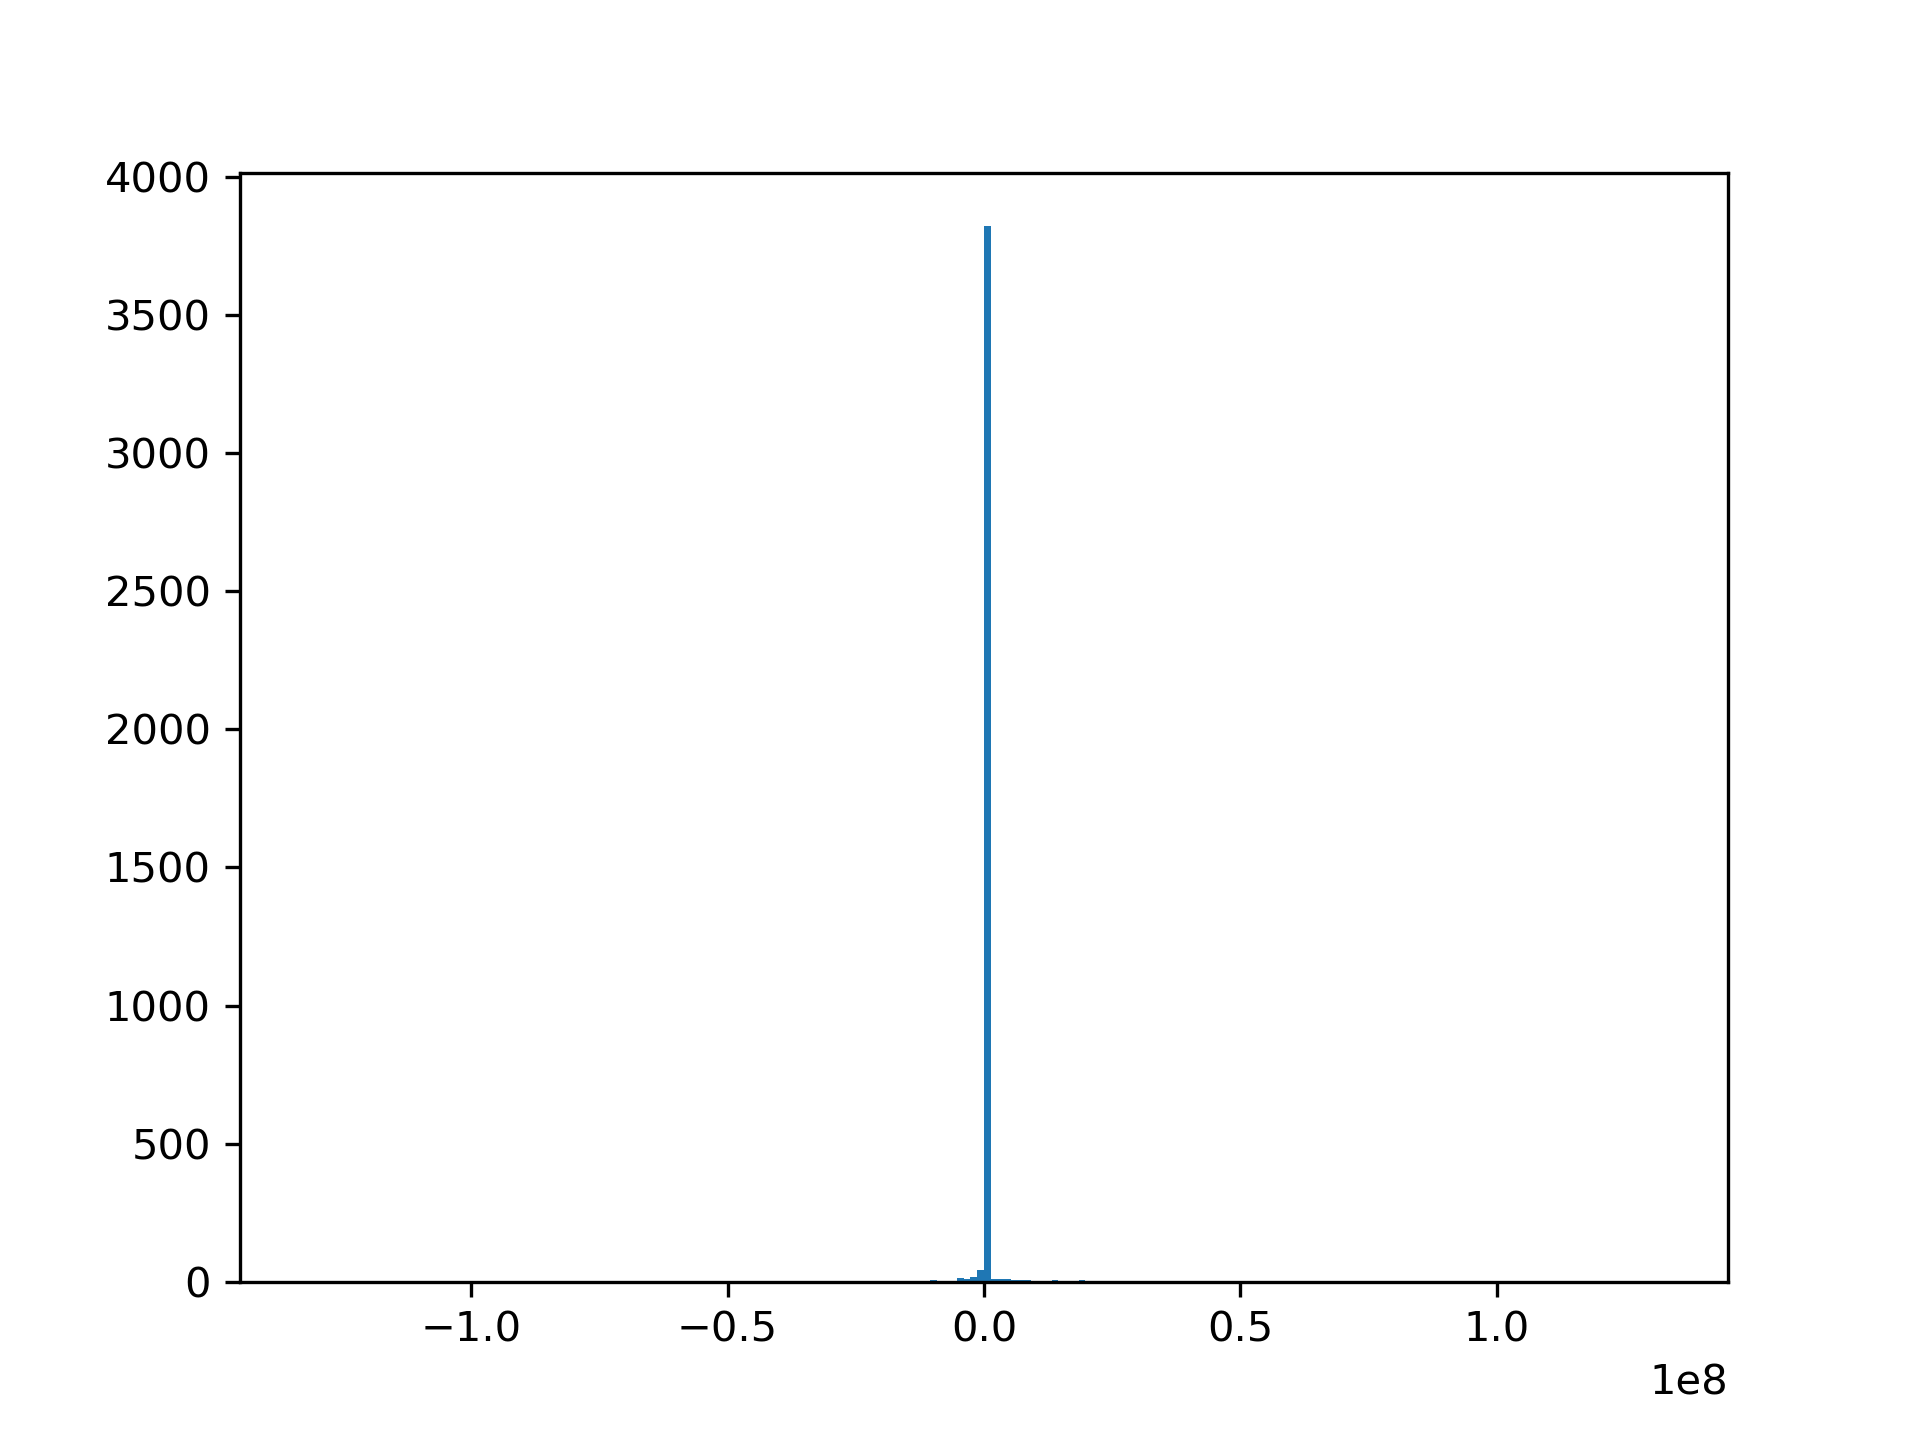
\includegraphics[width=\linewidth]{variables/Net Income - Discontinued ops.png}
    \caption{Histogram Net Income - Discontinued ops }
\end{figure}\section{ Net Income }

\begin{center}
    \begin{tabular}{|c | c|} 
    \hline
    Statystyka & Wartość \\
    \hline\hline
    Średnia arytmetyczna & 436364312.9865785 \\ 
    \hline
    Odchylenie standardowe & 2070648888.9140155 \\
    \hline
    Kwartyl dolny & -10668378.787875 \\
    \hline
    Mediana & 23713000.0 \\
    \hline
    Kwartyl górny & 191997000.0 \\
    \hline
    Wartość najmniejsza & -22355000000.0 \\
    \hline
    Wartość największa & 59531000000.0 \\
    \hline
   \end{tabular}
\end{center}

\begin{figure}[h!]
    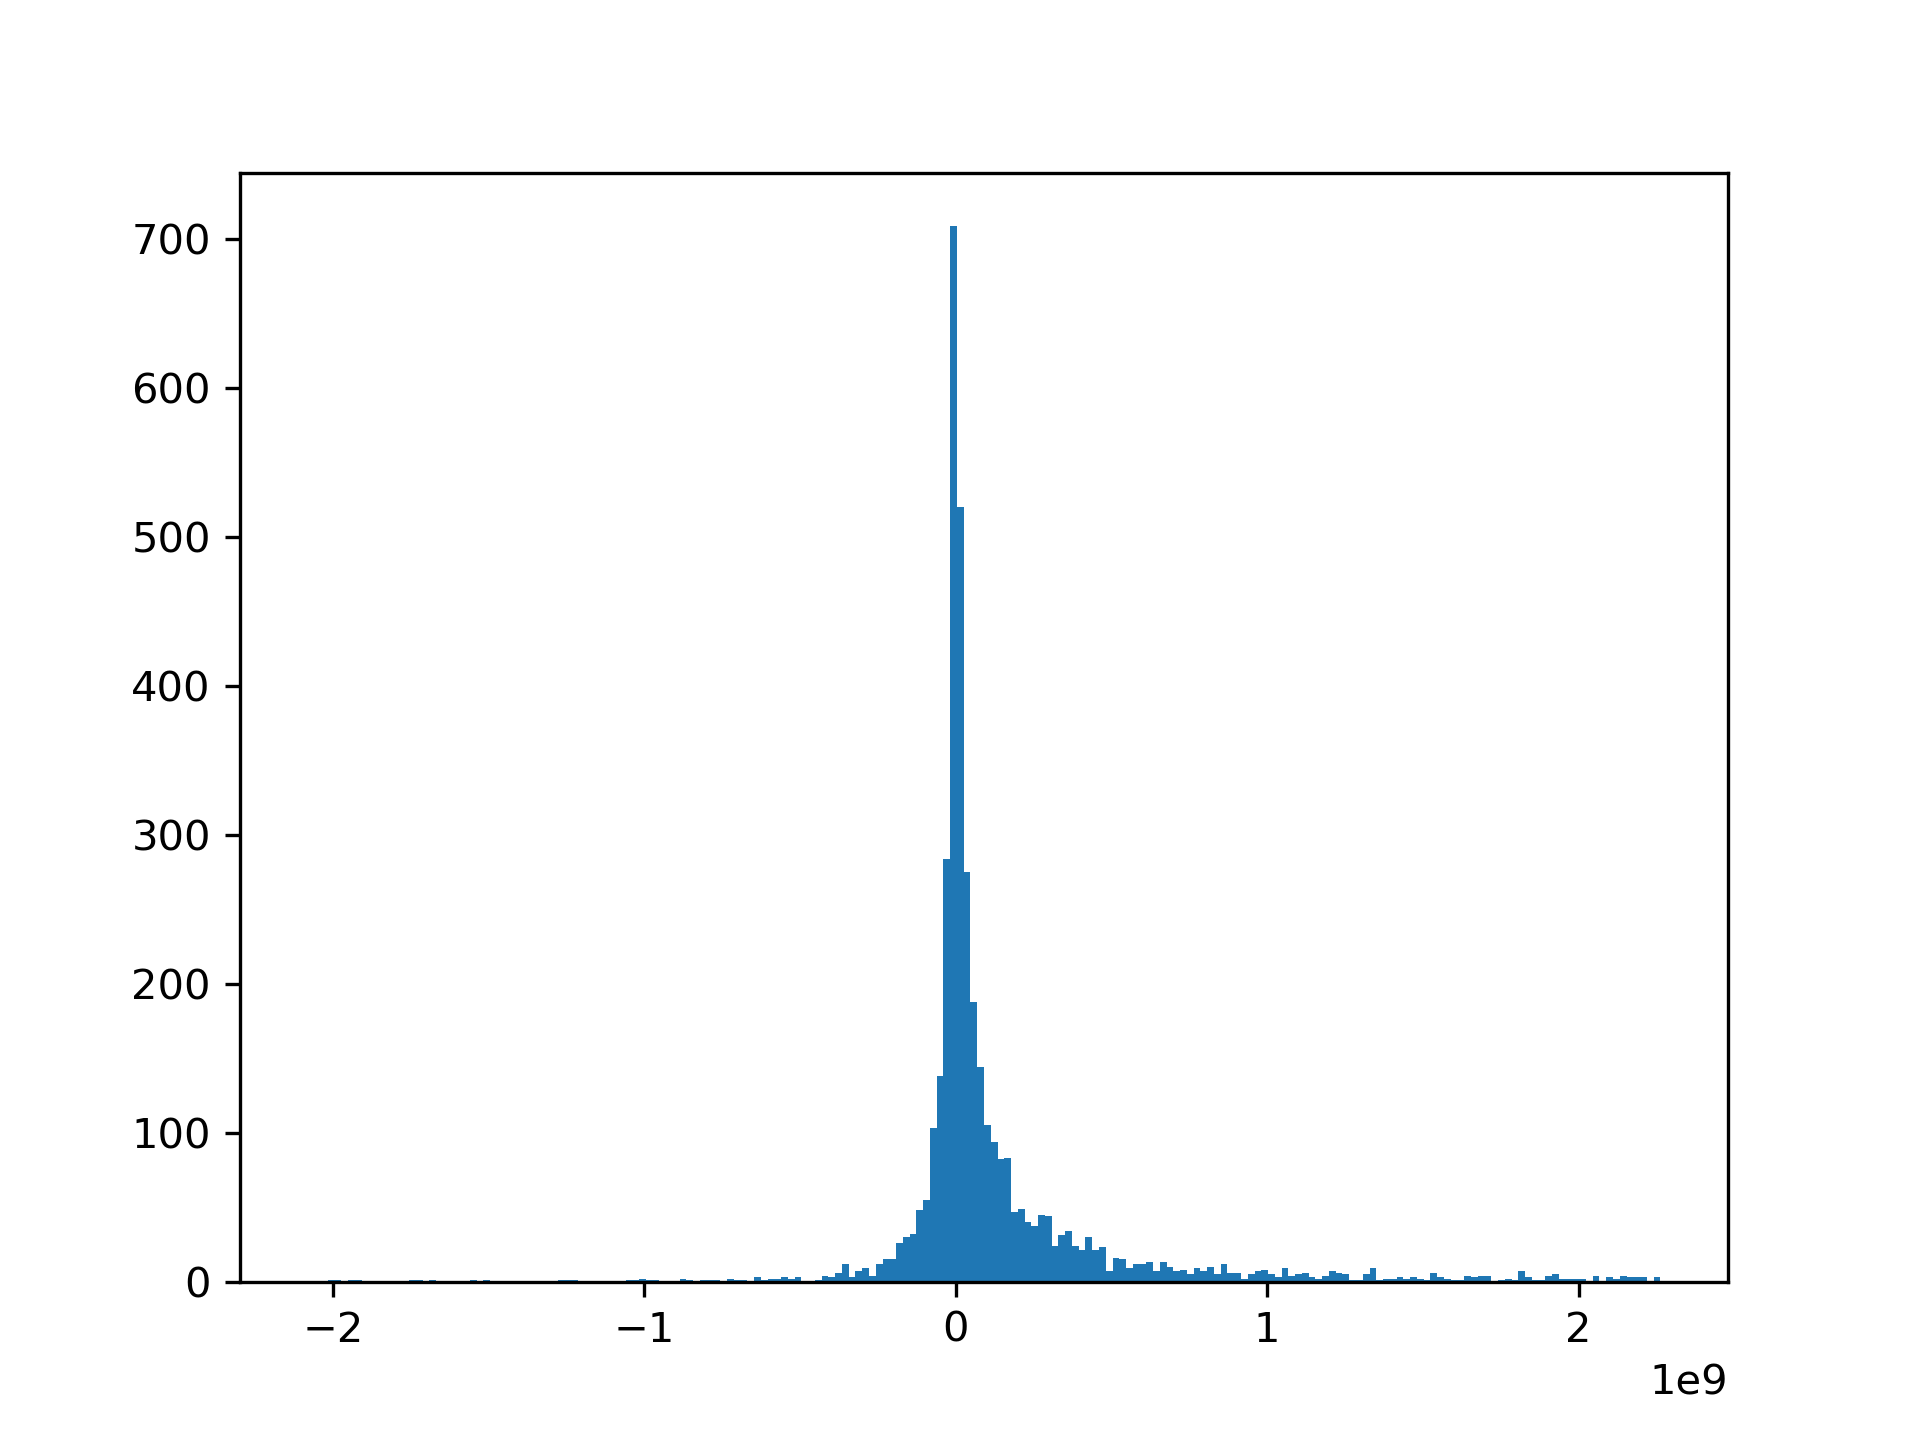
\includegraphics[width=\linewidth]{variables/Net Income.png}
    \caption{Histogram Net Income }
\end{figure}\section{ Preferred Dividends }

\begin{center}
    \begin{tabular}{|c | c|} 
    \hline
    Statystyka & Wartość \\
    \hline\hline
    Średnia arytmetyczna & 4619029.260465793 \\ 
    \hline
    Odchylenie standardowe & 46124349.31504317 \\
    \hline
    Kwartyl dolny & 0.0 \\
    \hline
    Mediana & 0.0 \\
    \hline
    Kwartyl górny & 0.0 \\
    \hline
    Wartość najmniejsza & -38330000.0 \\
    \hline
    Wartość największa & 1704000000.0 \\
    \hline
   \end{tabular}
\end{center}

\begin{figure}[h!]
    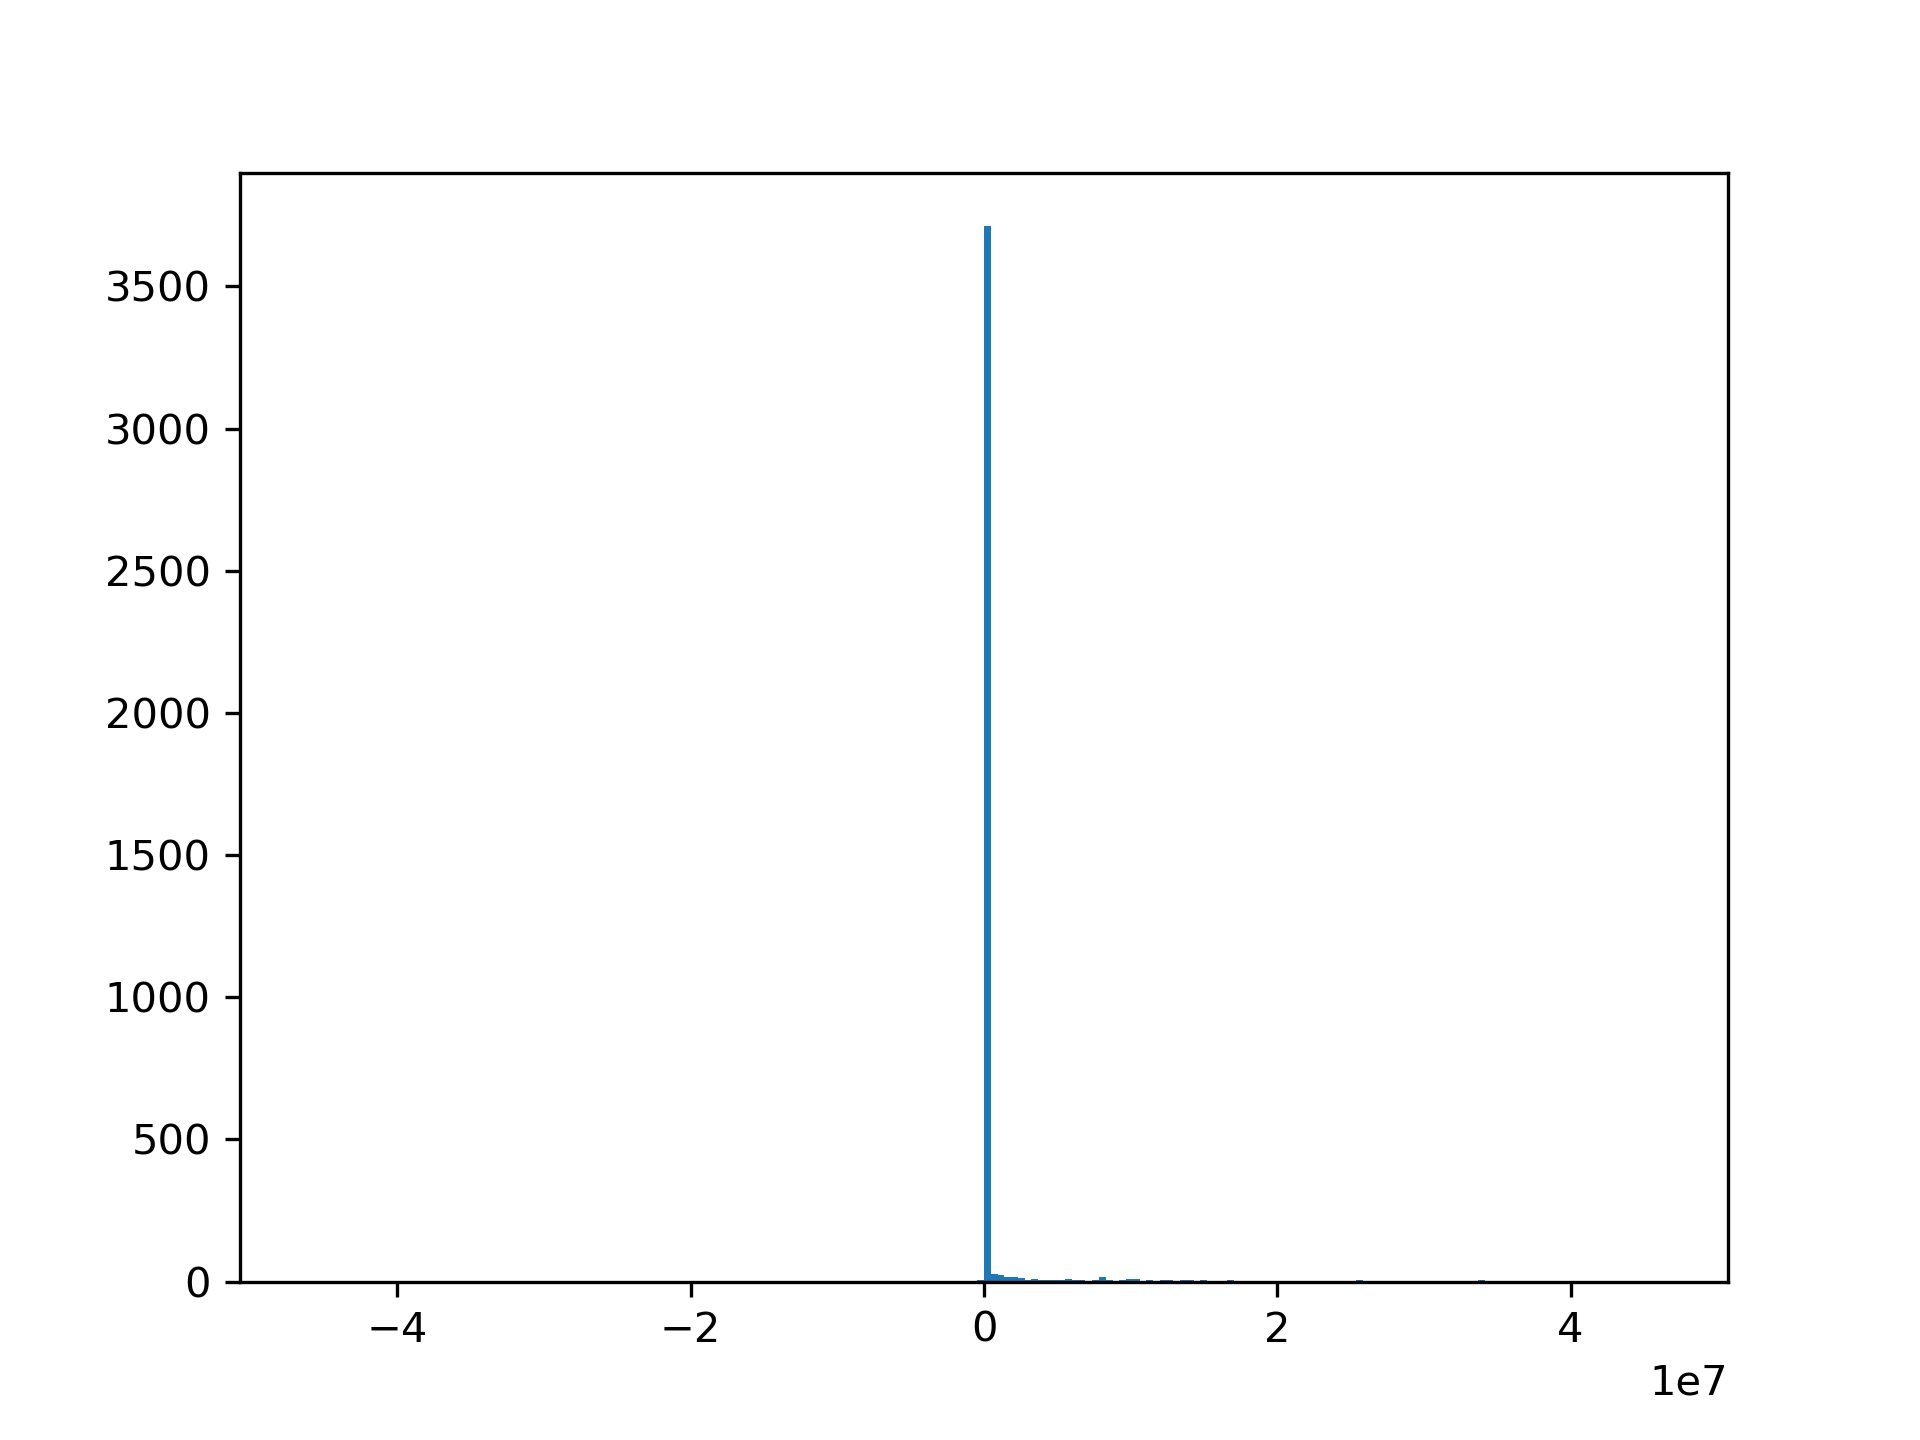
\includegraphics[width=\linewidth]{variables/Preferred Dividends.png}
    \caption{Histogram Preferred Dividends }
\end{figure}\section{ Net Income Com }

\begin{center}
    \begin{tabular}{|c | c|} 
    \hline
    Statystyka & Wartość \\
    \hline\hline
    Średnia arytmetyczna & 432841688.9945347 \\ 
    \hline
    Odchylenie standardowe & 2059355978.6405752 \\
    \hline
    Kwartyl dolny & -11318637.0 \\
    \hline
    Mediana & 22568764.7059 \\
    \hline
    Kwartyl górny & 190033000.0 \\
    \hline
    Wartość najmniejsza & -22802000000.0 \\
    \hline
    Wartość największa & 59531000000.0 \\
    \hline
   \end{tabular}
\end{center}

\begin{figure}[h!]
    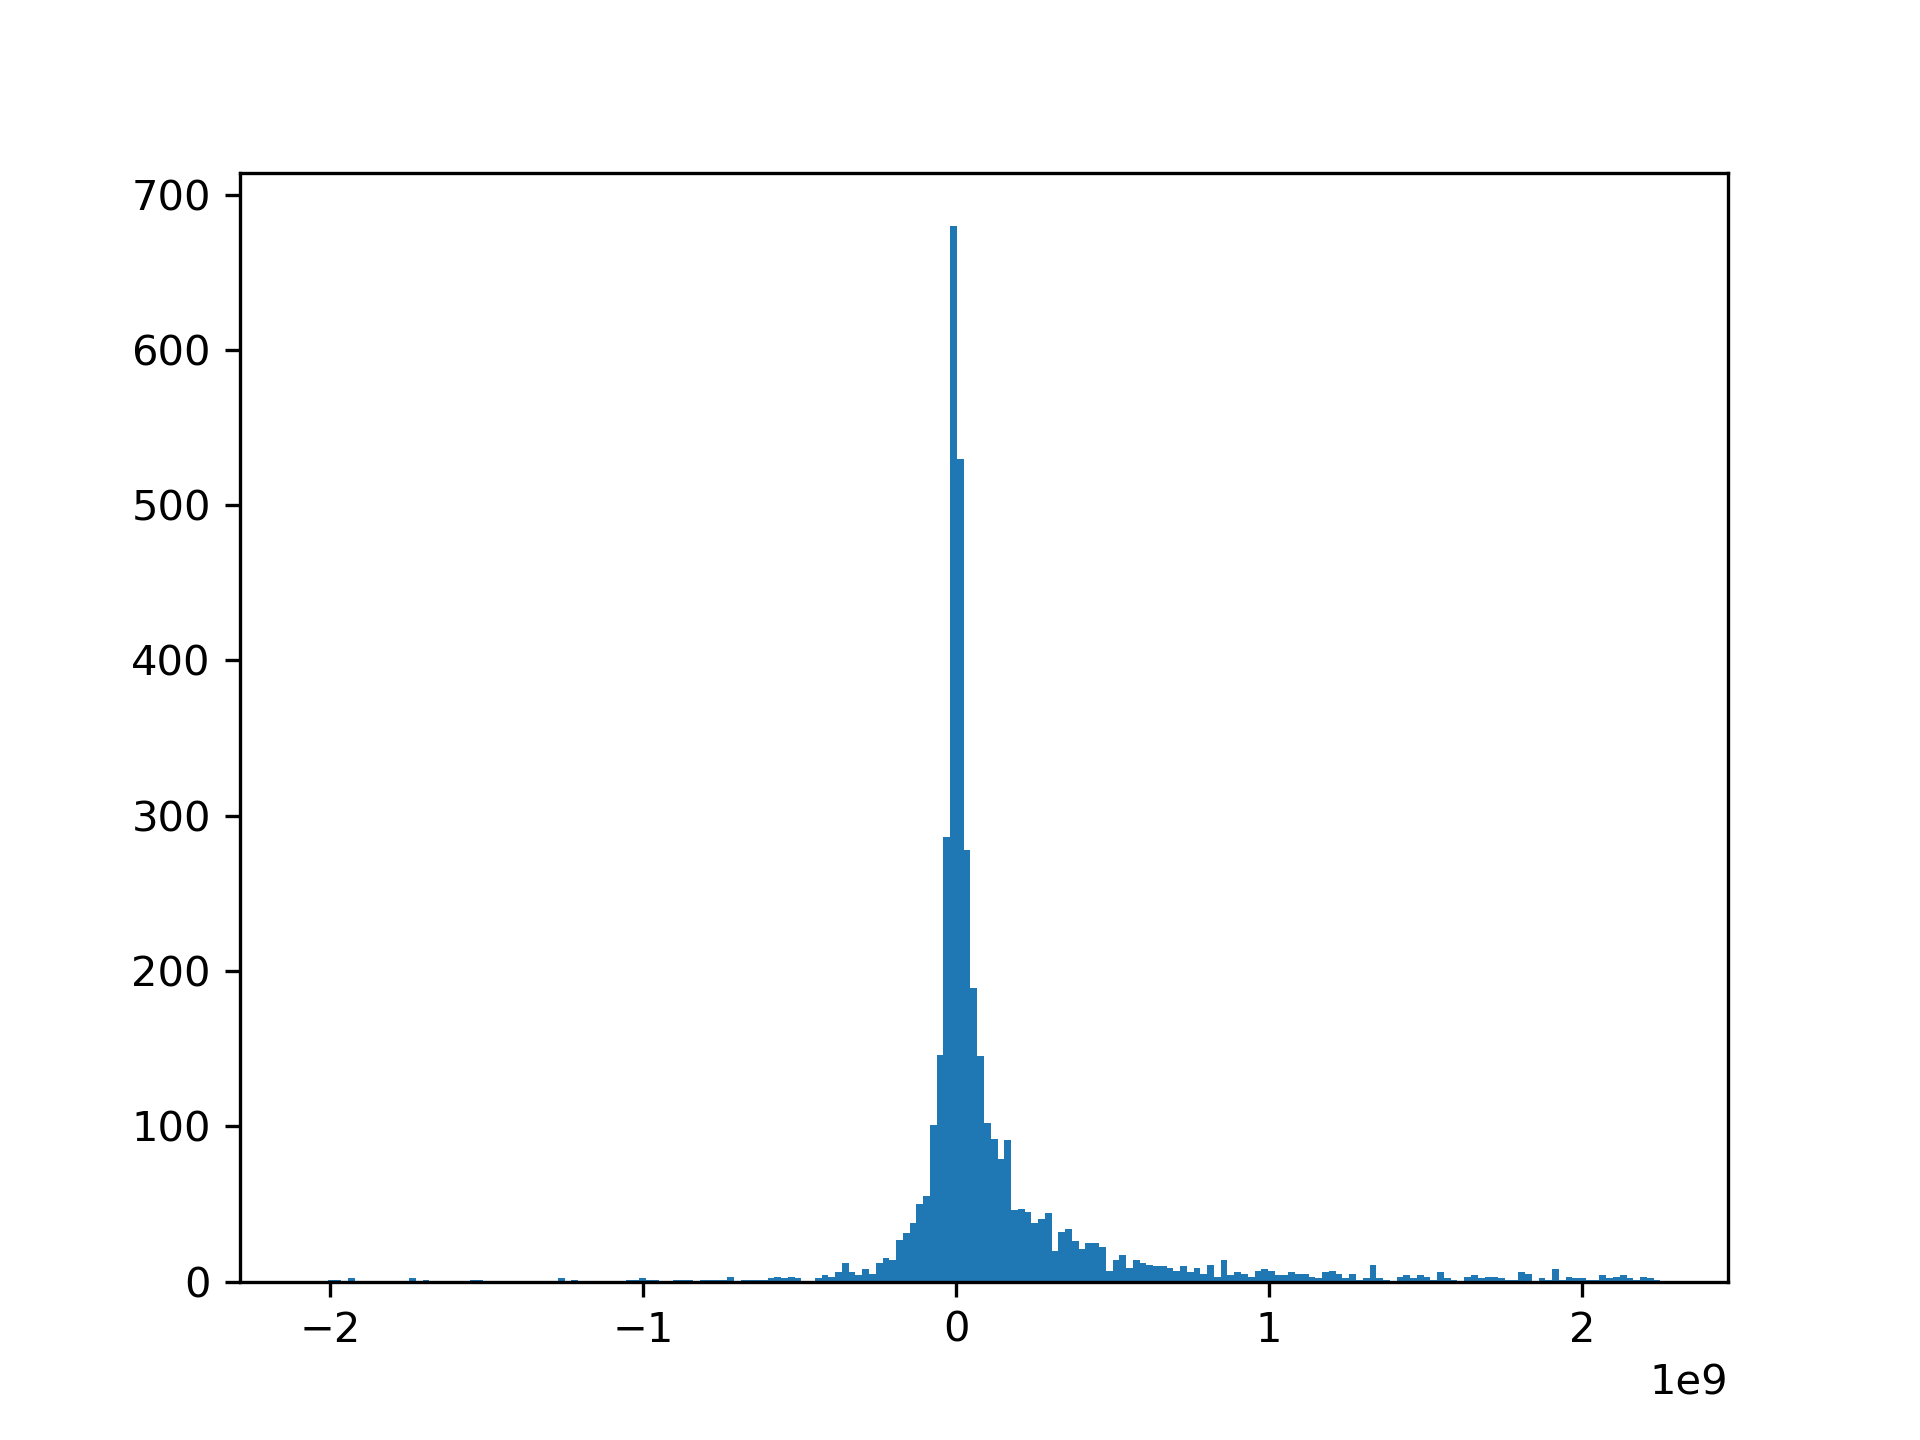
\includegraphics[width=\linewidth]{variables/Net Income Com.png}
    \caption{Histogram Net Income Com }
\end{figure}\section{ EPS }

\begin{center}
    \begin{tabular}{|c | c|} 
    \hline
    Statystyka & Wartość \\
    \hline\hline
    Średnia arytmetyczna & -73.477091436196 \\ 
    \hline
    Odchylenie standardowe & 5859.18379778386 \\
    \hline
    Kwartyl dolny & -0.39 \\
    \hline
    Mediana & 0.73 \\
    \hline
    Kwartyl górny & 2.38 \\
    \hline
    Wartość najmniejsza & -359825.0 \\
    \hline
    Wartość największa & 101641.0 \\
    \hline
   \end{tabular}
\end{center}

\begin{figure}[h!]
    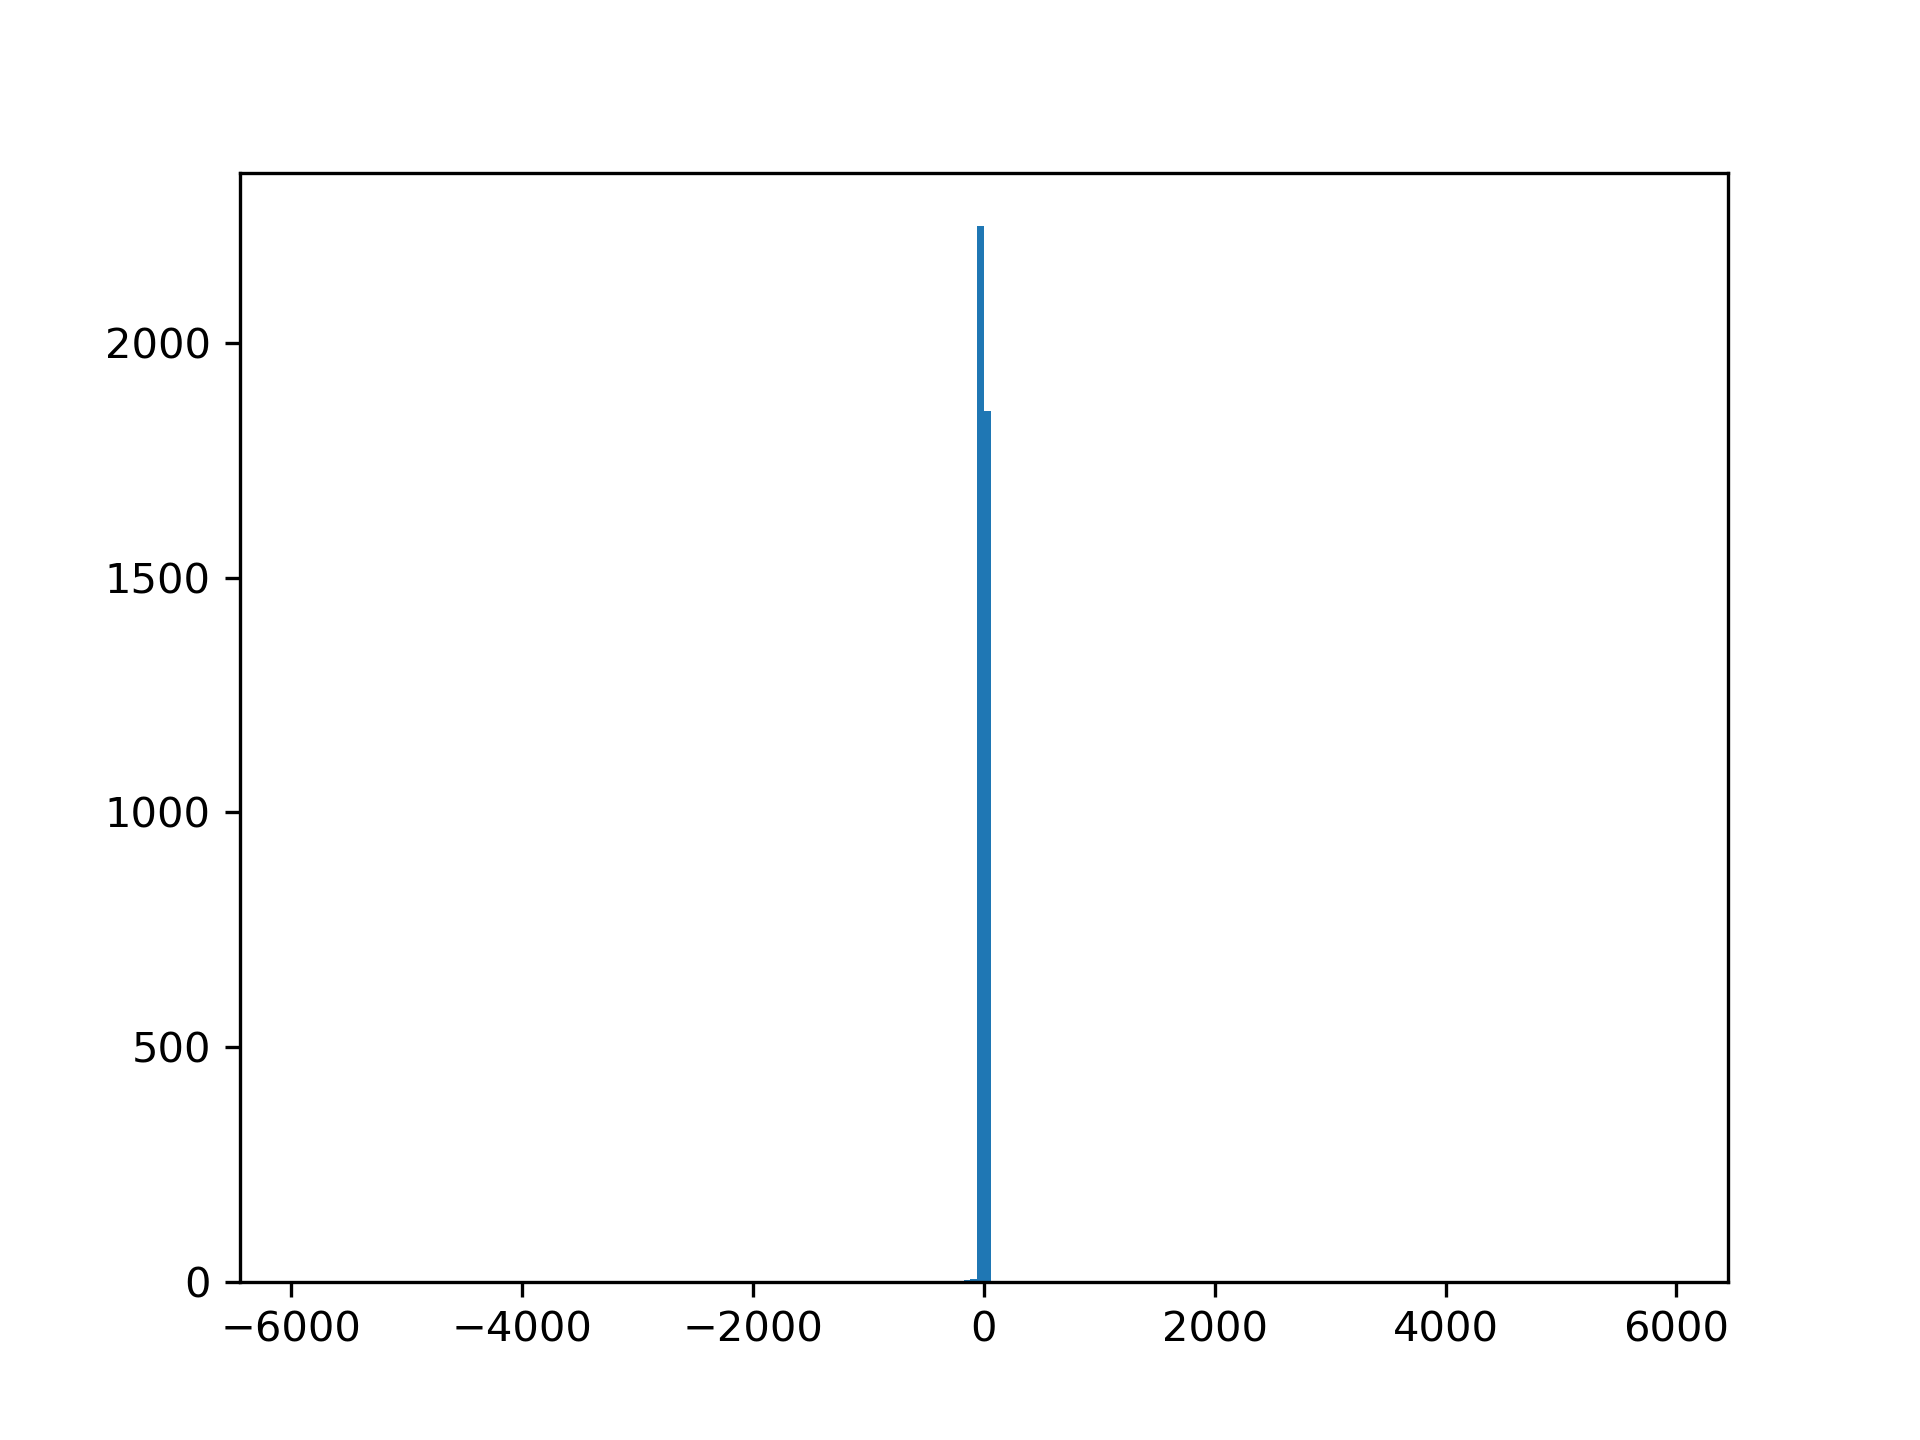
\includegraphics[width=\linewidth]{variables/EPS.png}
    \caption{Histogram EPS }
\end{figure}\section{ EPS Diluted }

\begin{center}
    \begin{tabular}{|c | c|} 
    \hline
    Statystyka & Wartość \\
    \hline\hline
    Średnia arytmetyczna & -75.07707142163997 \\ 
    \hline
    Odchylenie standardowe & 5832.97438887803 \\
    \hline
    Kwartyl dolny & -0.39 \\
    \hline
    Mediana & 0.72 \\
    \hline
    Kwartyl górny & 2.32 \\
    \hline
    Wartość najmniejsza & -359825.0 \\
    \hline
    Wartość największa & 95231.4433 \\
    \hline
   \end{tabular}
\end{center}

\begin{figure}[h!]
    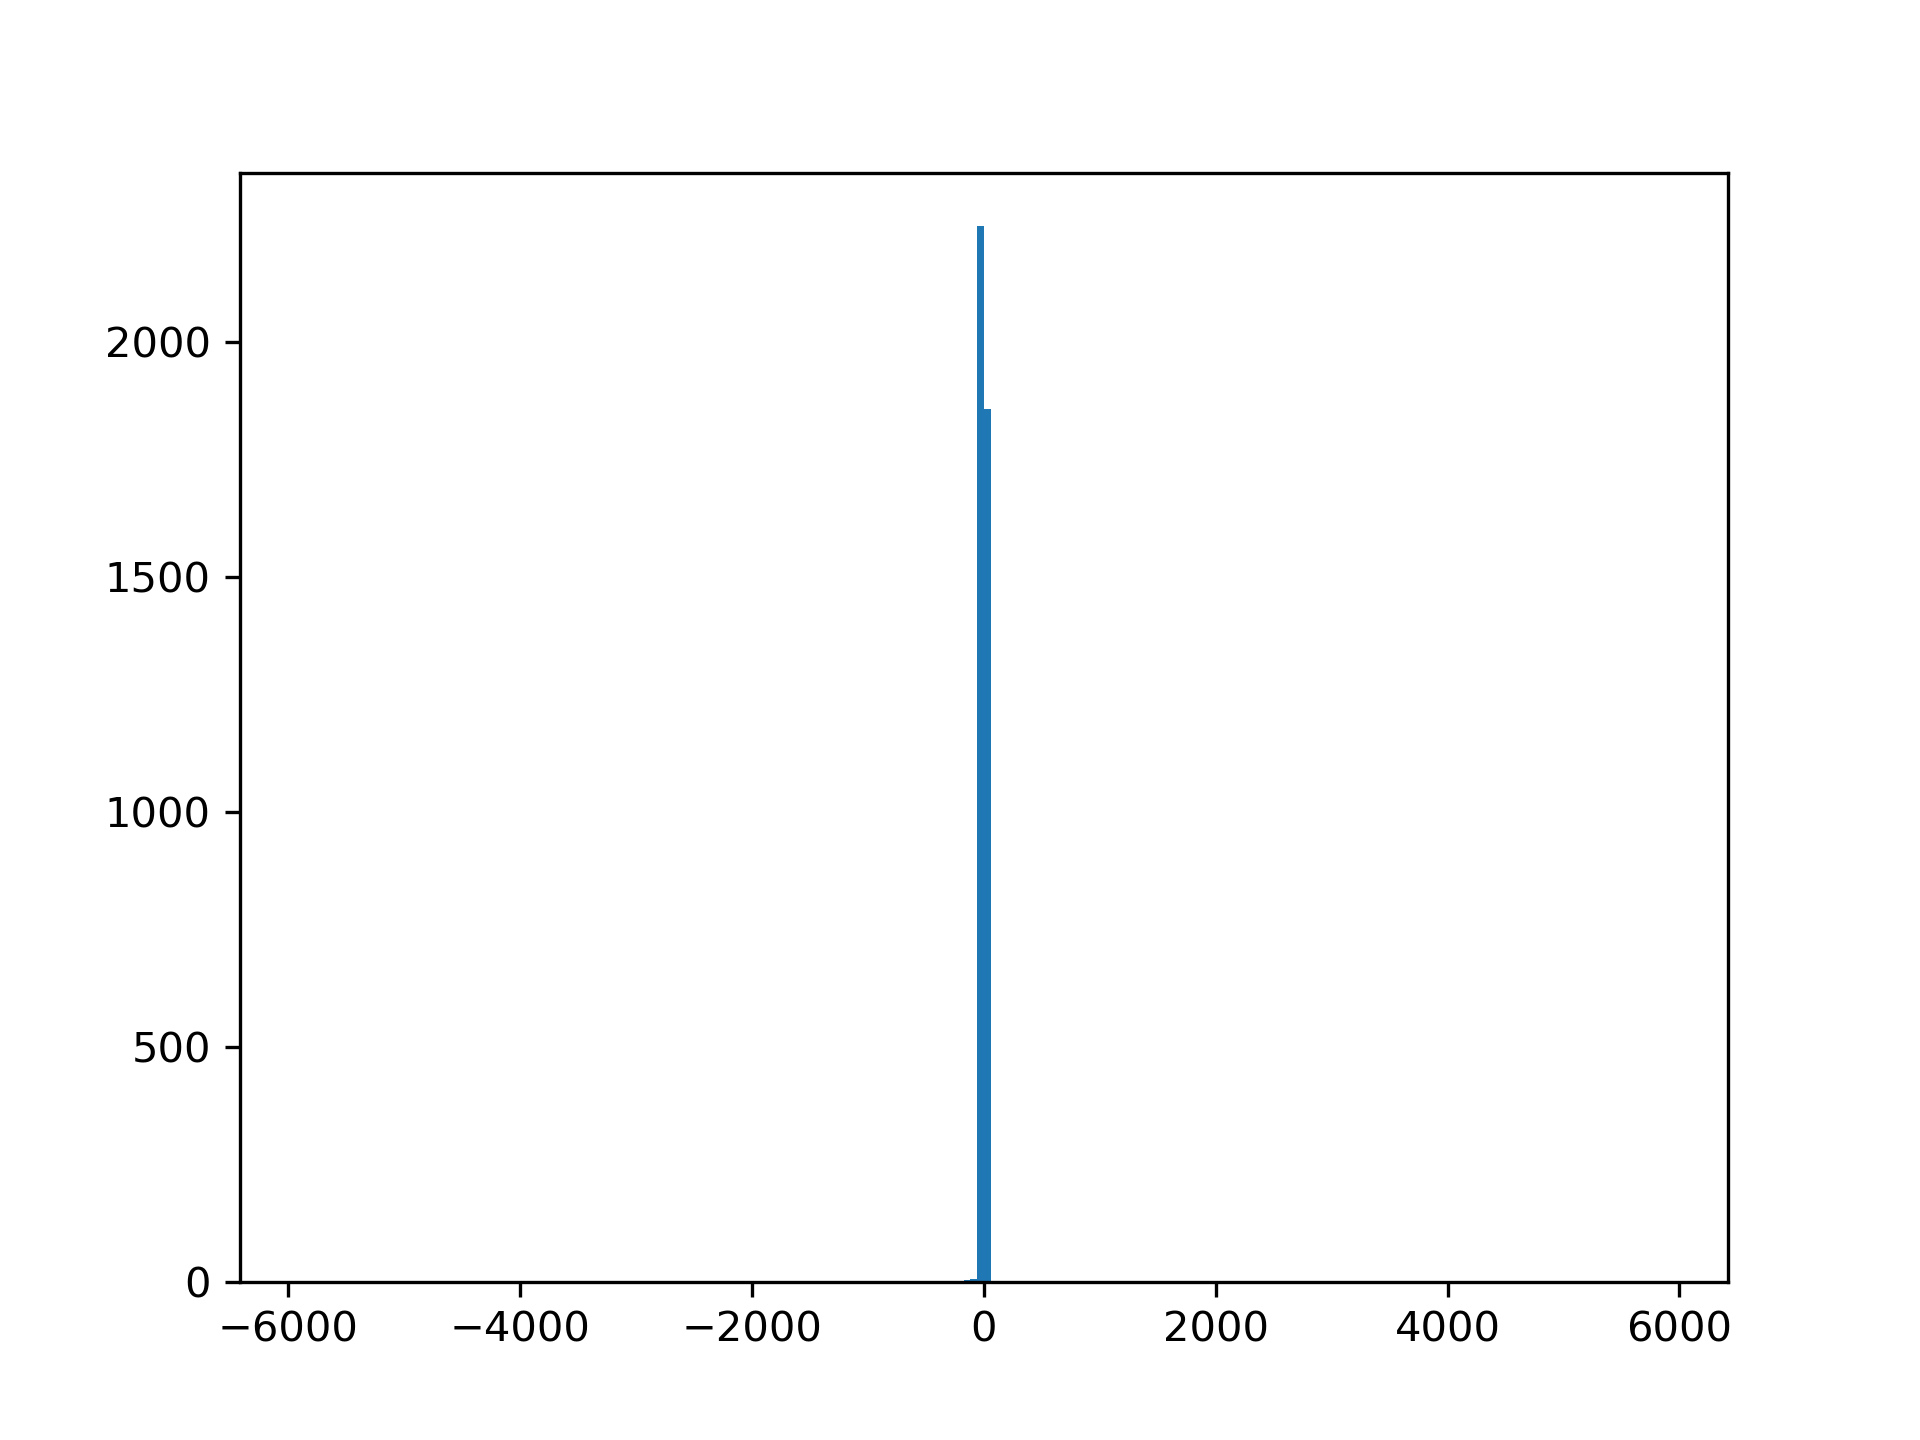
\includegraphics[width=\linewidth]{variables/EPS Diluted.png}
    \caption{Histogram EPS Diluted }
\end{figure}\section{ Weighted Average Shs Out }

\begin{center}
    \begin{tabular}{|c | c|} 
    \hline
    Statystyka & Wartość \\
    \hline\hline
    Średnia arytmetyczna & 265307317.10912618 \\ 
    \hline
    Odchylenie standardowe & 2053723952.1842713 \\
    \hline
    Kwartyl dolny & 19648933.5 \\
    \hline
    Mediana & 47418953.00855 \\
    \hline
    Kwartyl górny & 126504008.25 \\
    \hline
    Wartość najmniejsza & 119.0 \\
    \hline
    Wartość największa & 91336230442.8934 \\
    \hline
   \end{tabular}
\end{center}

\begin{figure}[h!]
    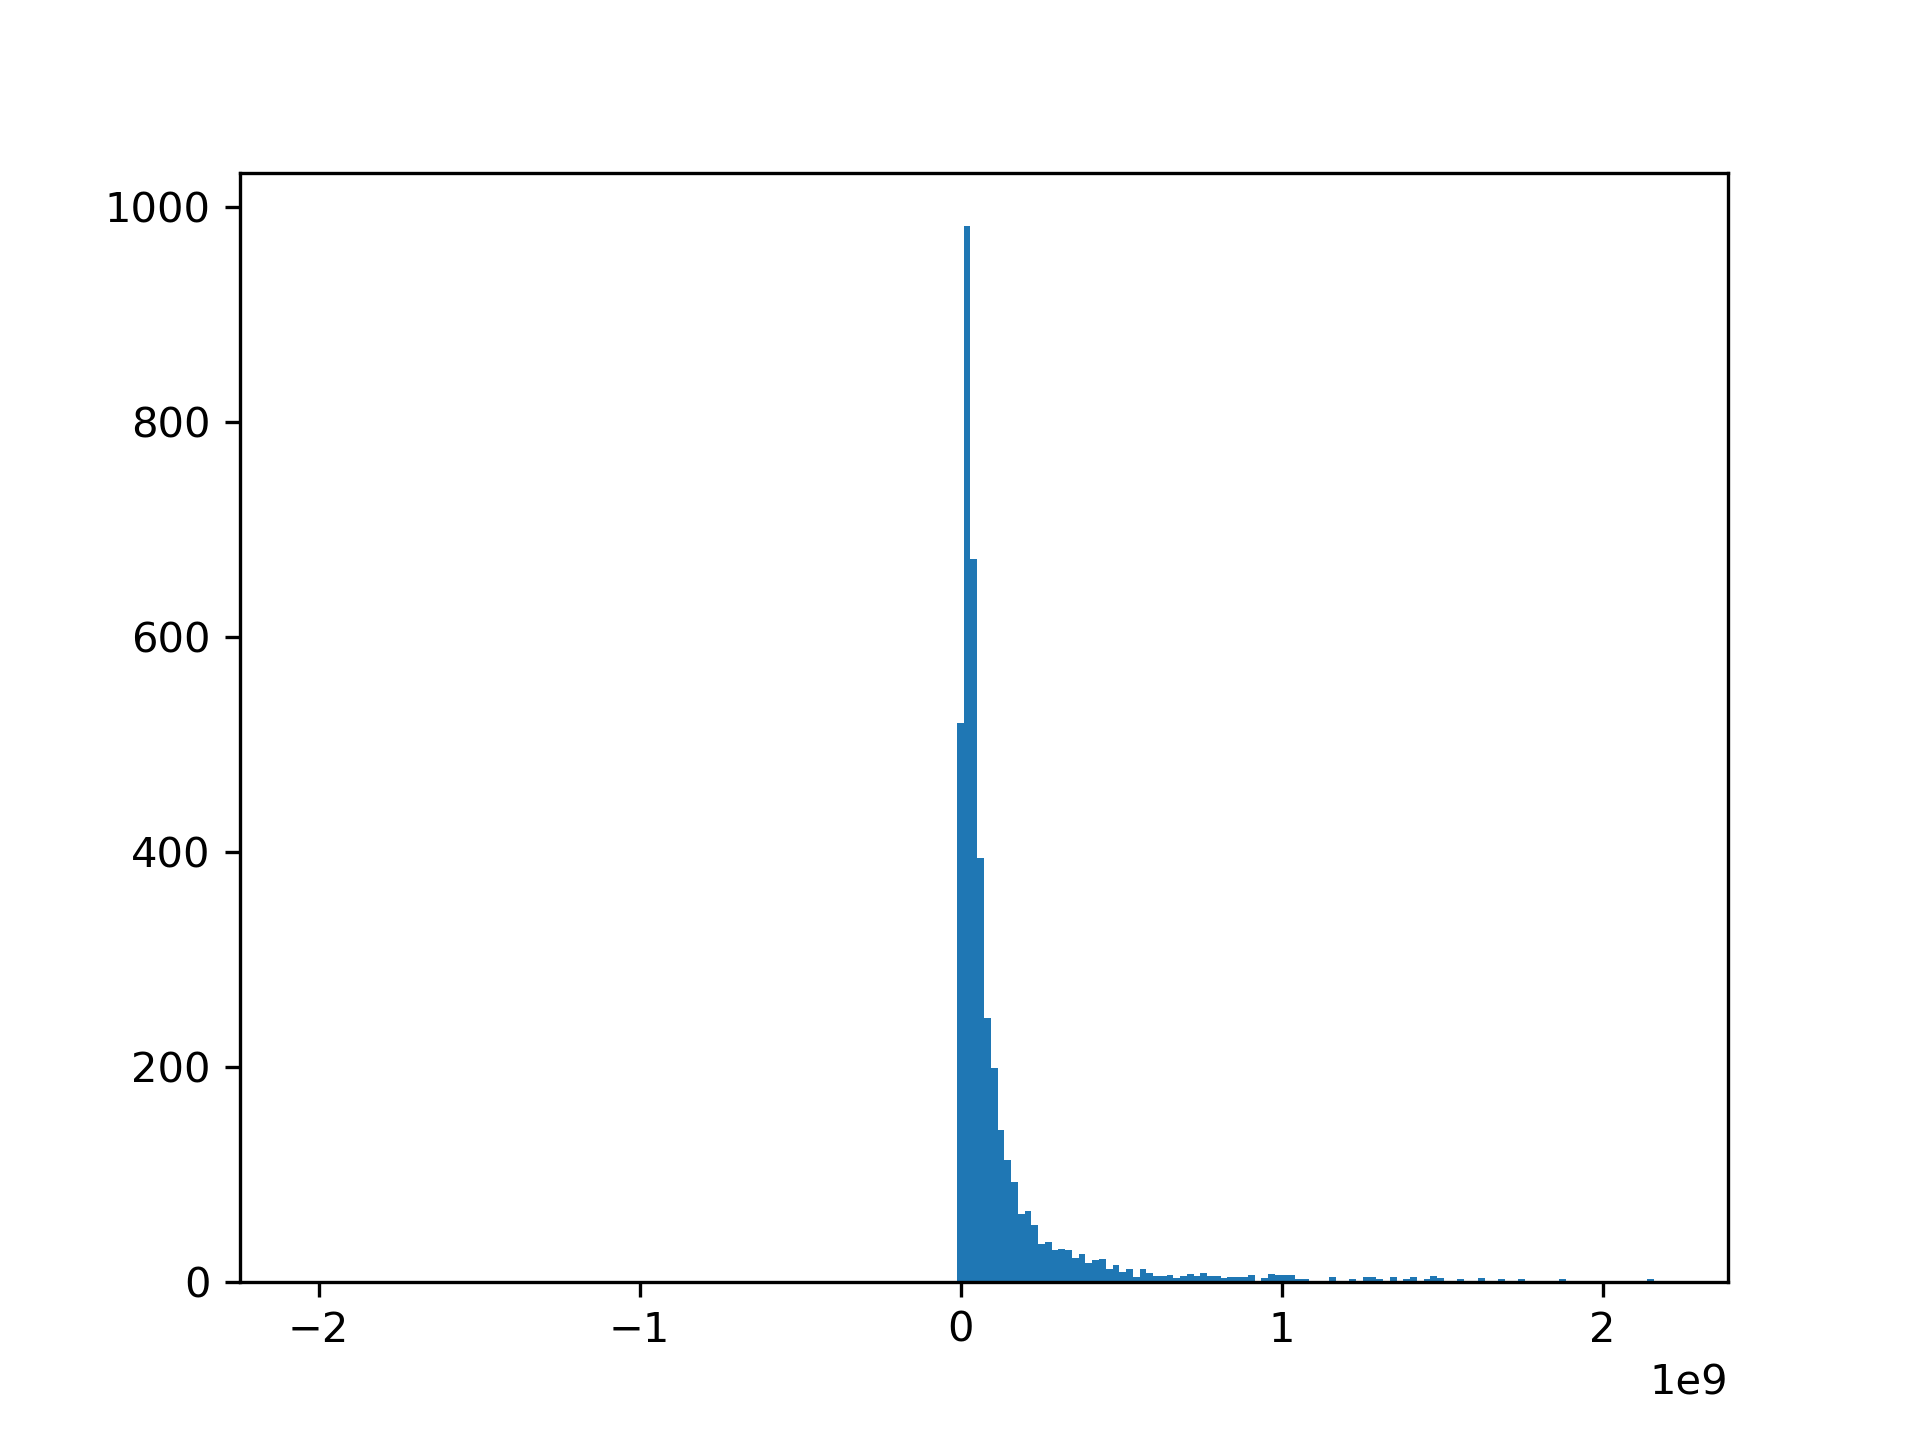
\includegraphics[width=\linewidth]{variables/Weighted Average Shs Out.png}
    \caption{Histogram Weighted Average Shs Out }
\end{figure}\section{ Weighted Average Shs Out (Dil) }

\begin{center}
    \begin{tabular}{|c | c|} 
    \hline
    Statystyka & Wartość \\
    \hline\hline
    Średnia arytmetyczna & 264316559.41049492 \\ 
    \hline
    Odchylenie standardowe & 2048408031.341803 \\
    \hline
    Kwartyl dolny & 19166299.5 \\
    \hline
    Mediana & 46450791.5 \\
    \hline
    Kwartyl górny & 123276500.0 \\
    \hline
    Wartość najmniejsza & 74.0 \\
    \hline
    Wartość największa & 91336230442.8934 \\
    \hline
   \end{tabular}
\end{center}

\begin{figure}[h!]
    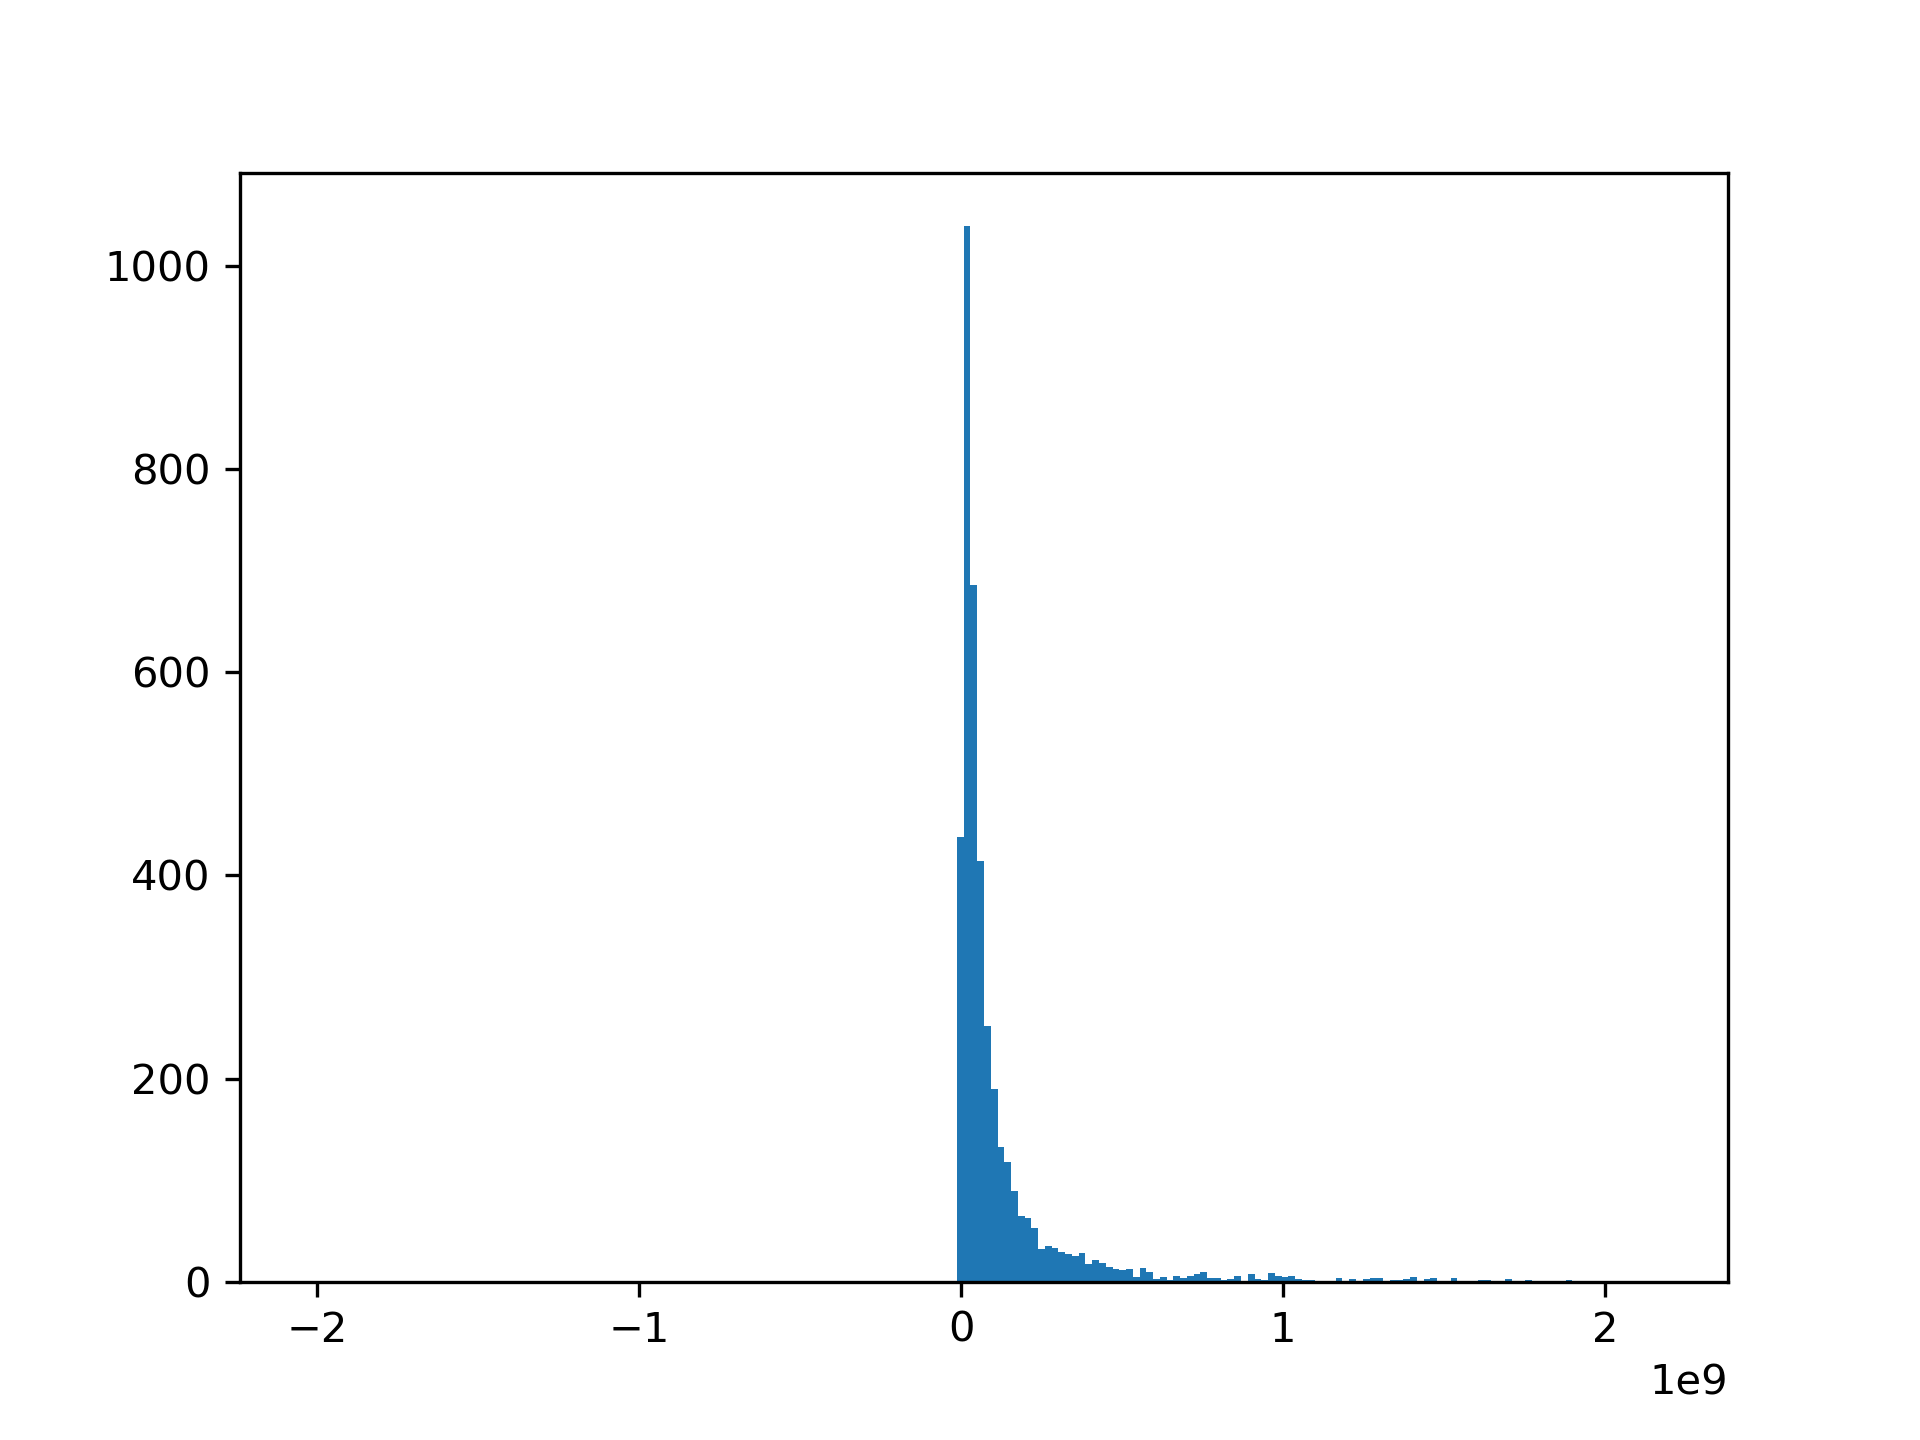
\includegraphics[width=\linewidth]{variables/Weighted Average Shs Out (Dil).png}
    \caption{Histogram Weighted Average Shs Out (Dil) }
\end{figure}\section{ Dividend per Share }

\begin{center}
    \begin{tabular}{|c | c|} 
    \hline
    Statystyka & Wartość \\
    \hline\hline
    Średnia arytmetyczna & 0.6130498544395925 \\ 
    \hline
    Odchylenie standardowe & 1.4455139737528337 \\
    \hline
    Kwartyl dolny & 0.0 \\
    \hline
    Mediana & 0.0 \\
    \hline
    Kwartyl górny & 0.8 \\
    \hline
    Wartość najmniejsza & 0.0 \\
    \hline
    Wartość największa & 45.305 \\
    \hline
   \end{tabular}
\end{center}

\begin{figure}[h!]
    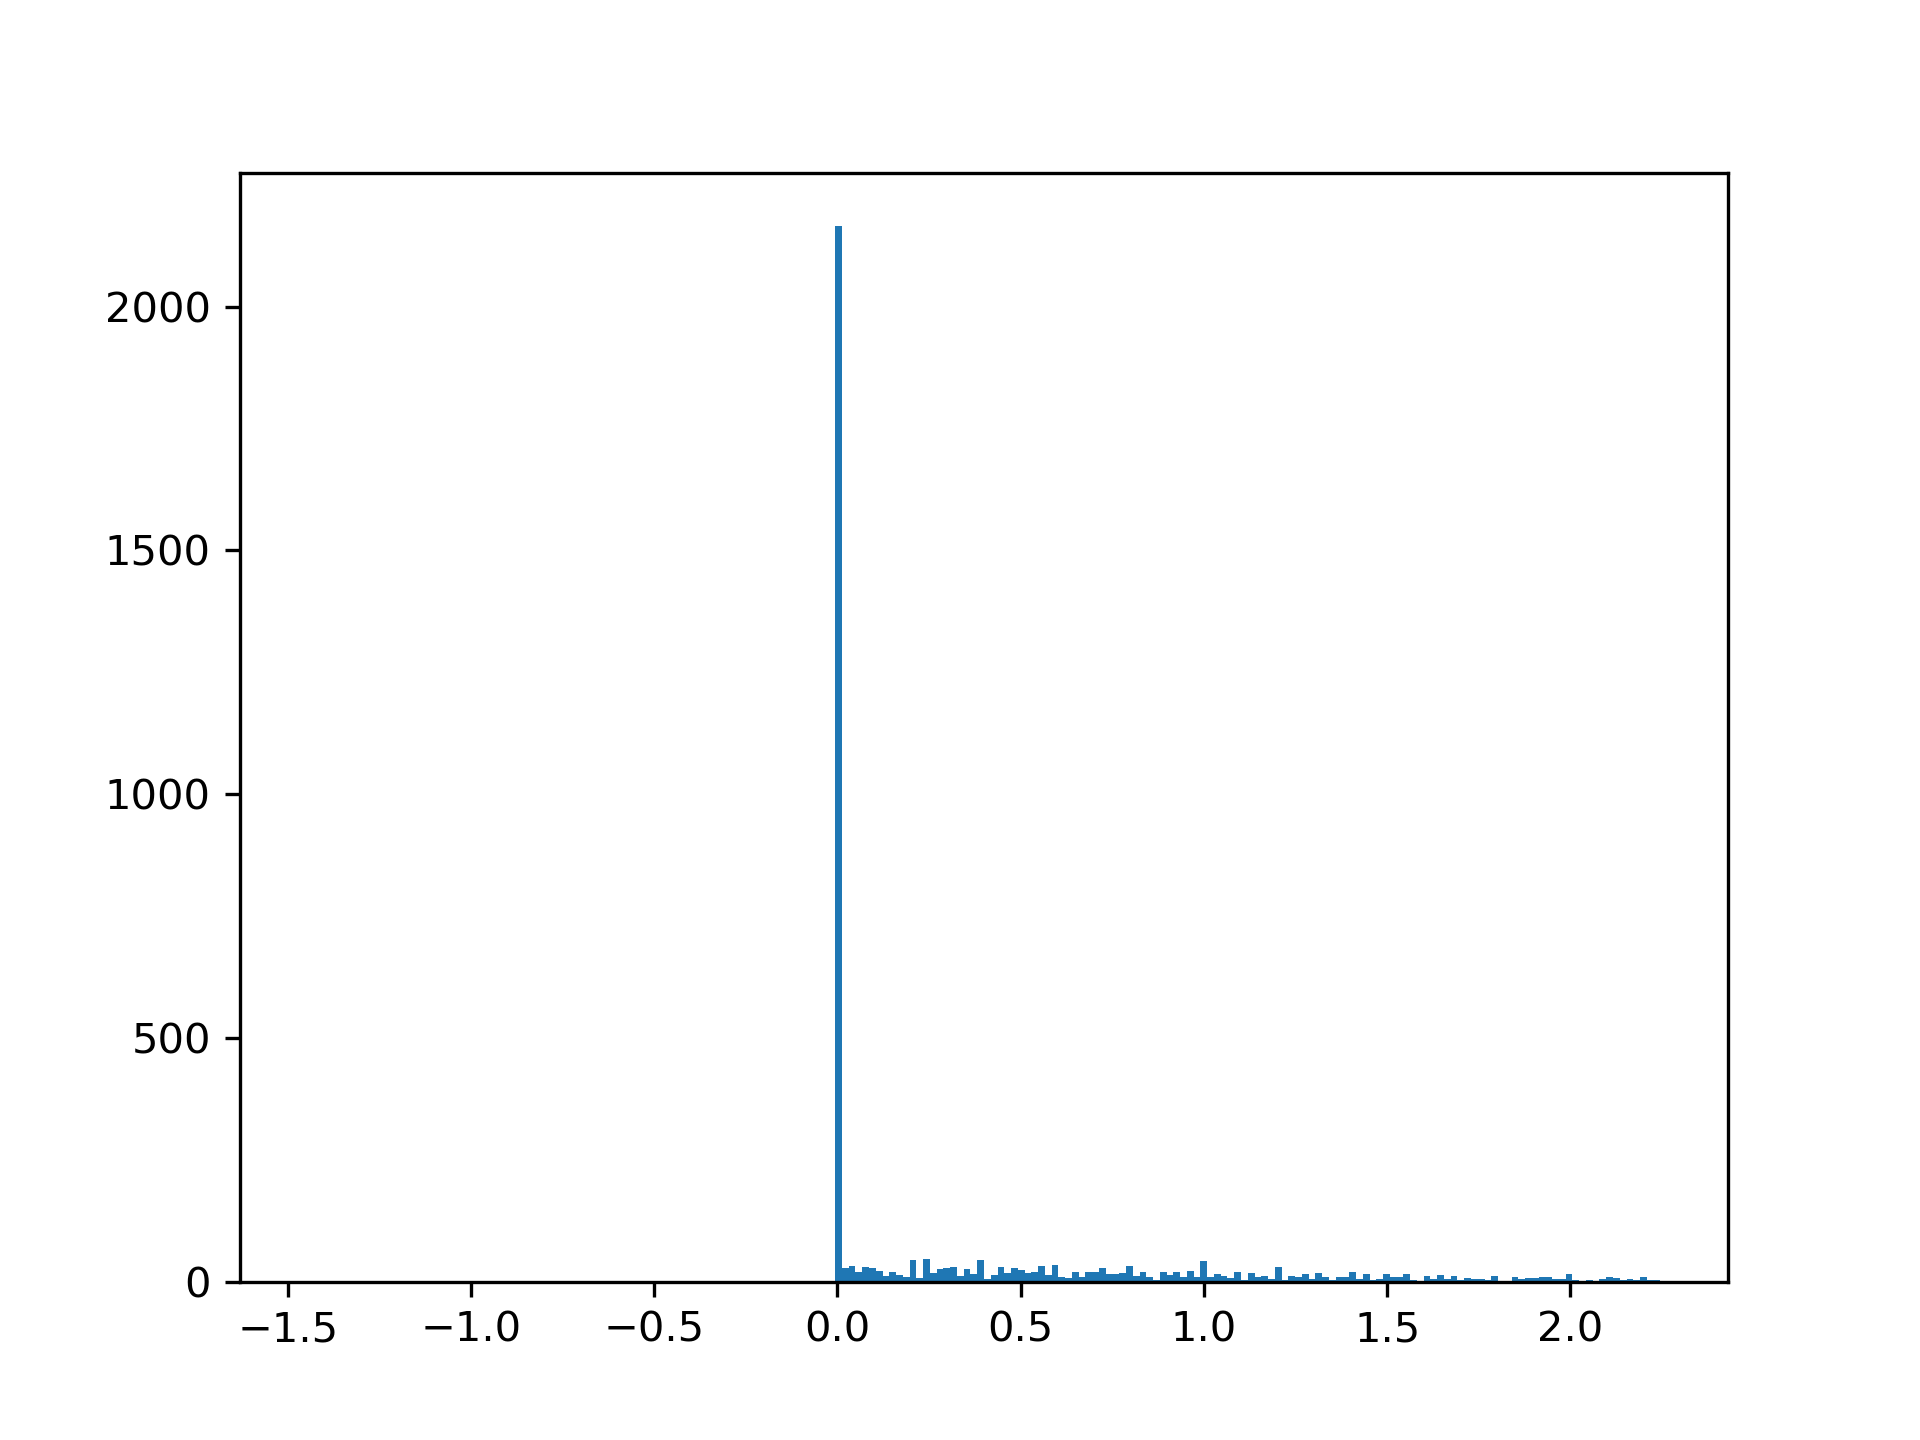
\includegraphics[width=\linewidth]{variables/Dividend per Share.png}
    \caption{Histogram Dividend per Share }
\end{figure}\section{ Gross Margin }

\begin{center}
    \begin{tabular}{|c | c|} 
    \hline
    Statystyka & Wartość \\
    \hline\hline
    Średnia arytmetyczna & 0.49076921397379913 \\ 
    \hline
    Odchylenie standardowe & 0.5901823736418663 \\
    \hline
    Kwartyl dolny & 0.253825 \\
    \hline
    Mediana & 0.4589 \\
    \hline
    Kwartyl górny & 0.783775 \\
    \hline
    Wartość najmniejsza & -19.9043 \\
    \hline
    Wartość największa & 1.8965 \\
    \hline
   \end{tabular}
\end{center}

\begin{figure}[h!]
    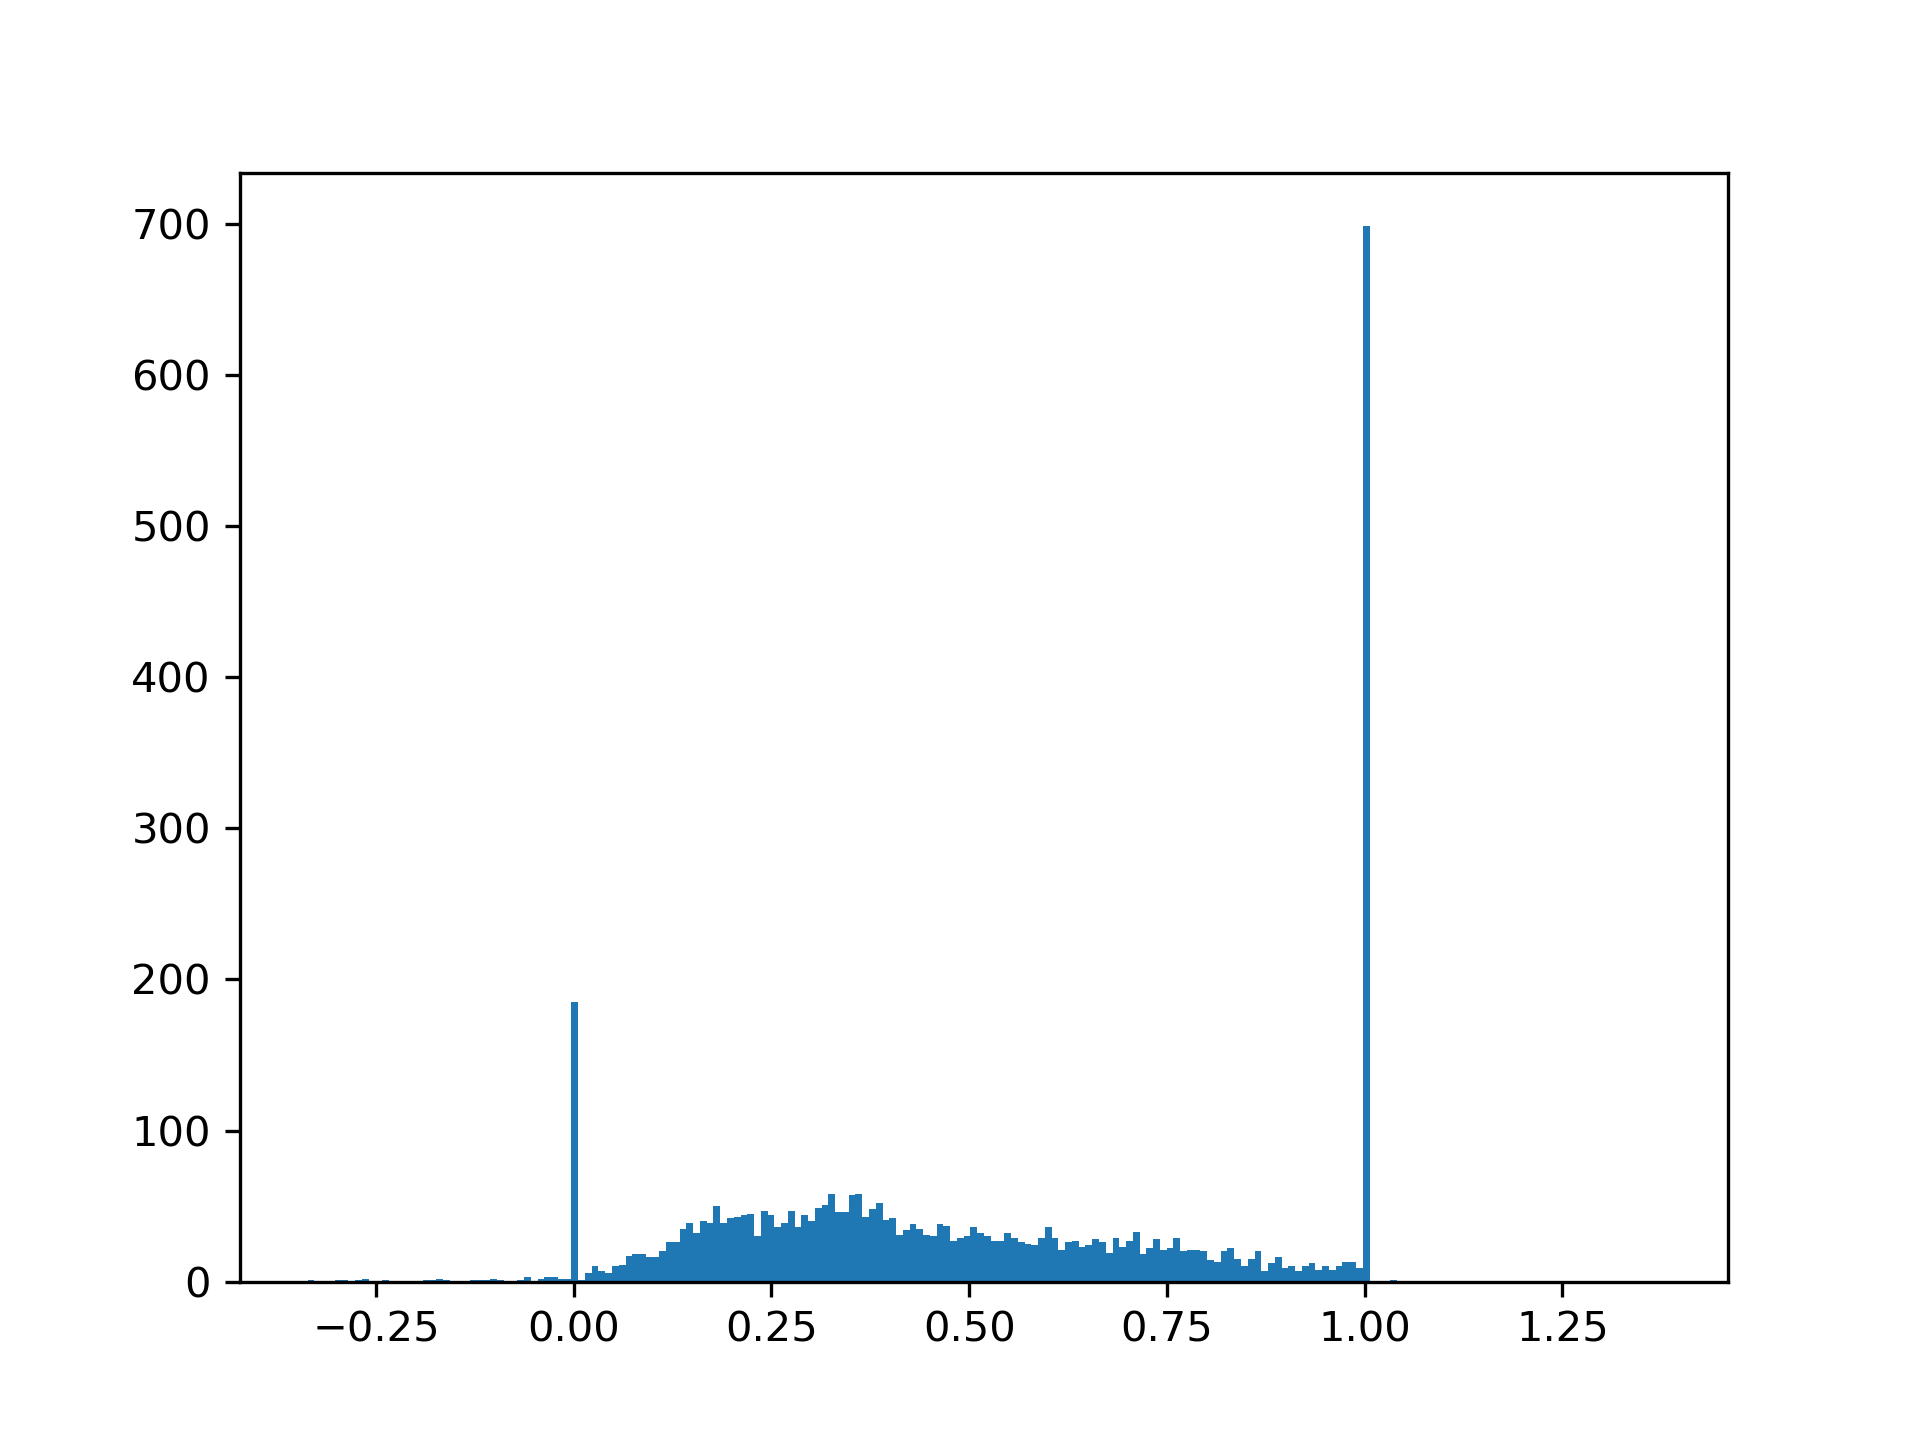
\includegraphics[width=\linewidth]{variables/Gross Margin.png}
    \caption{Histogram Gross Margin }
\end{figure}\section{ EBITDA Margin }

\begin{center}
    \begin{tabular}{|c | c|} 
    \hline
    Statystyka & Wartość \\
    \hline\hline
    Średnia arytmetyczna & -8.888892049999999 \\ 
    \hline
    Odchylenie standardowe & 175.17794788771585 \\
    \hline
    Kwartyl dolny & 0.005125 \\
    \hline
    Mediana & 0.12300000000000001 \\
    \hline
    Kwartyl górny & 0.299 \\
    \hline
    Wartość najmniejsza & -8809.838 \\
    \hline
    Wartość największa & 1060.404 \\
    \hline
   \end{tabular}
\end{center}

\begin{figure}[h!]
    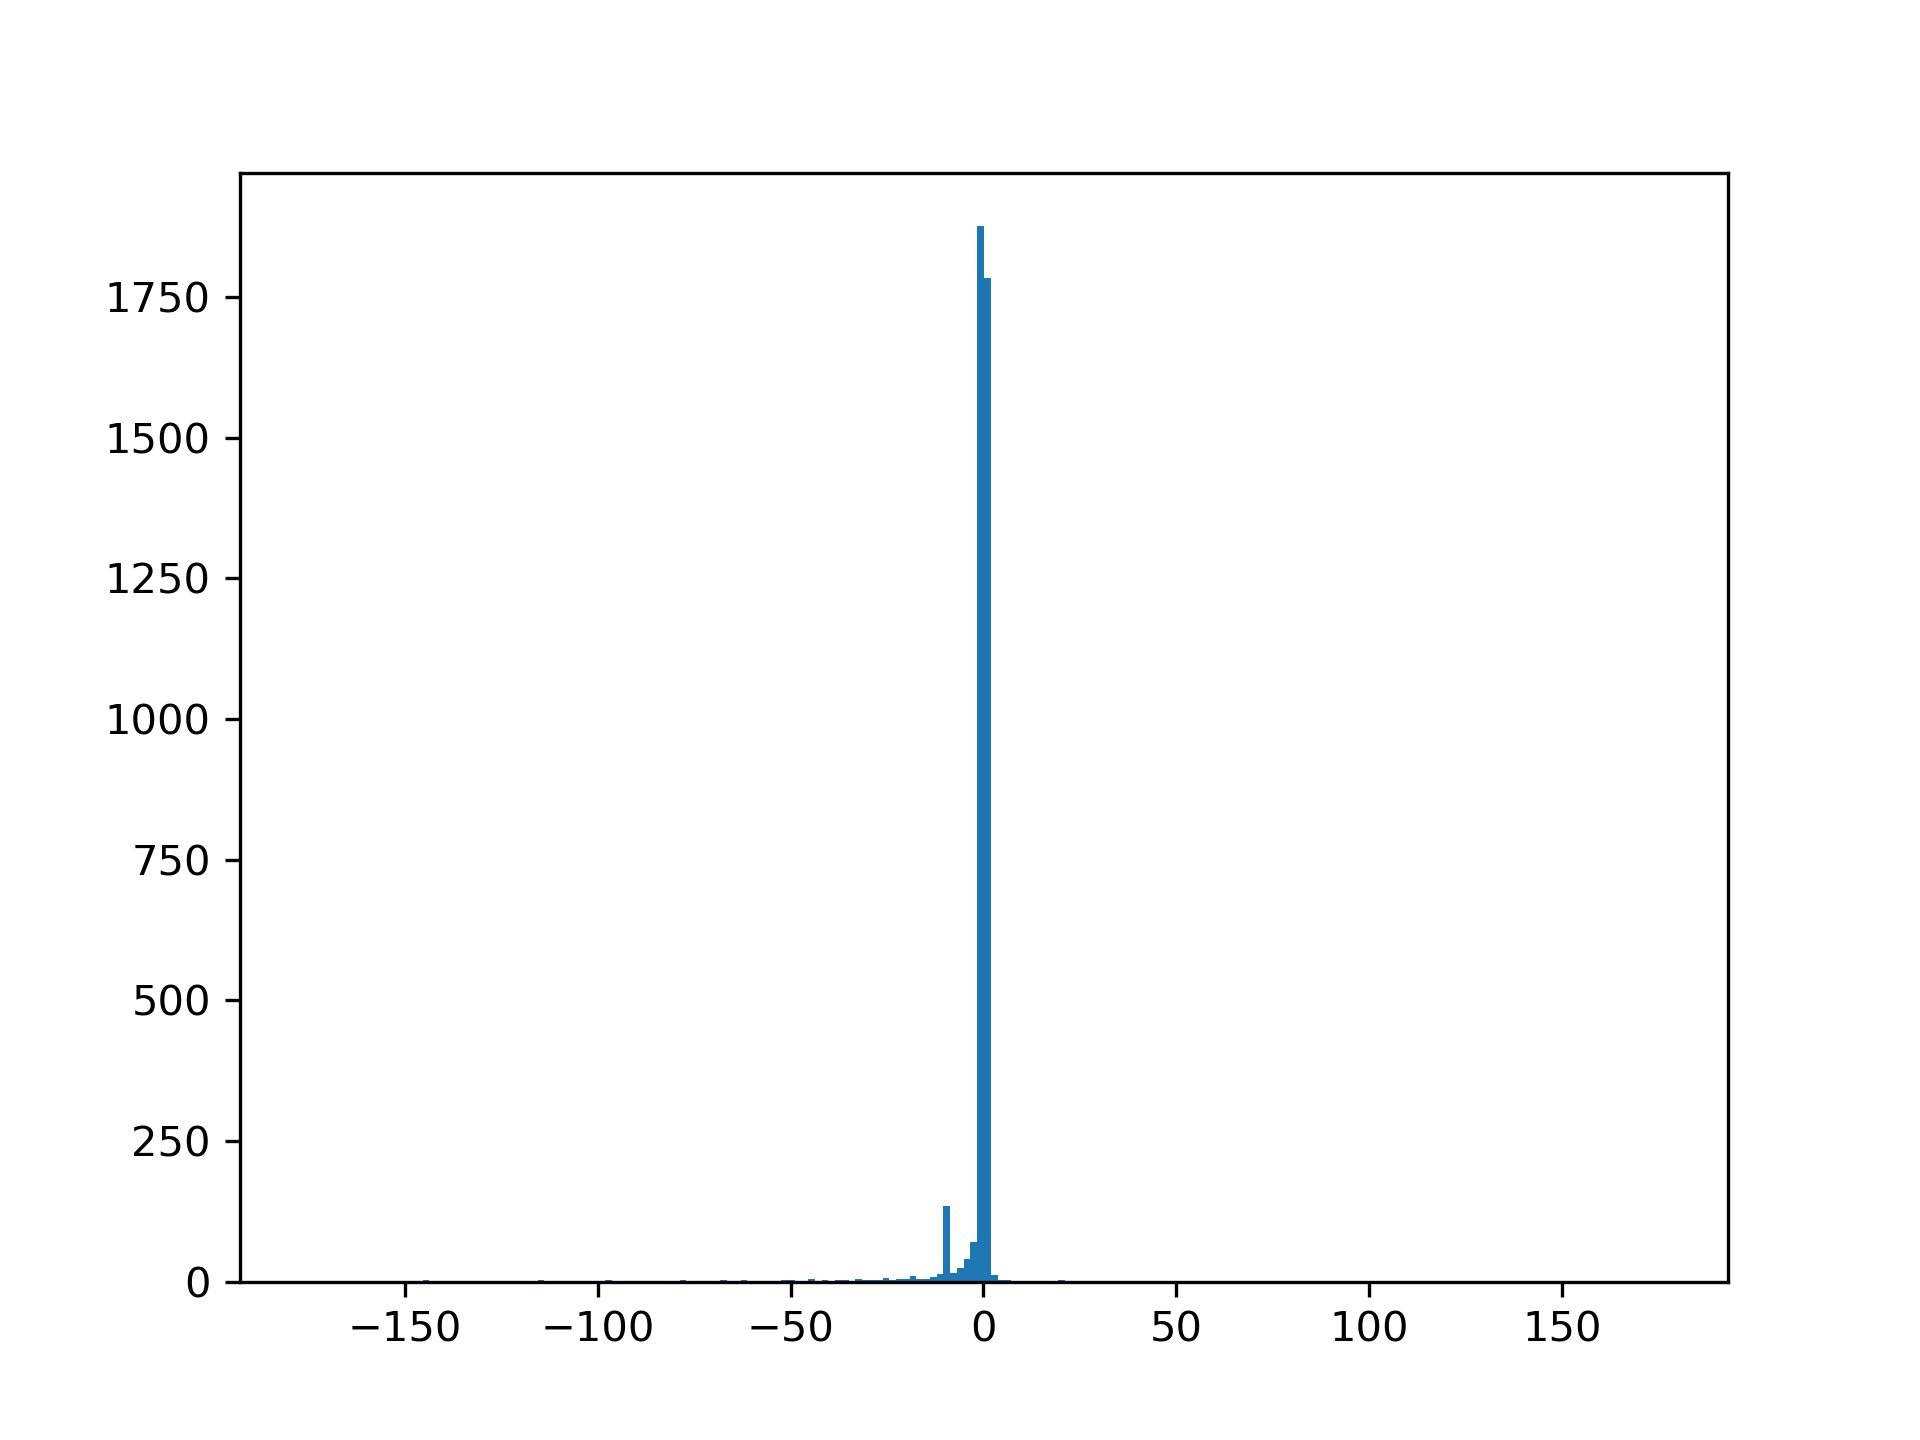
\includegraphics[width=\linewidth]{variables/EBITDA Margin.png}
    \caption{Histogram EBITDA Margin }
\end{figure}\section{ EBIT Margin }

\begin{center}
    \begin{tabular}{|c | c|} 
    \hline
    Statystyka & Wartość \\
    \hline\hline
    Średnia arytmetyczna & -4.940808102862688 \\ 
    \hline
    Odchylenie standardowe & 104.70221985541568 \\
    \hline
    Kwartyl dolny & 0.0 \\
    \hline
    Mediana & 0.08024999999999999 \\
    \hline
    Kwartyl górny & 0.21675 \\
    \hline
    Wartość najmniejsza & -5009.1667 \\
    \hline
    Wartość największa & 1056.4658 \\
    \hline
   \end{tabular}
\end{center}

\begin{figure}[h!]
    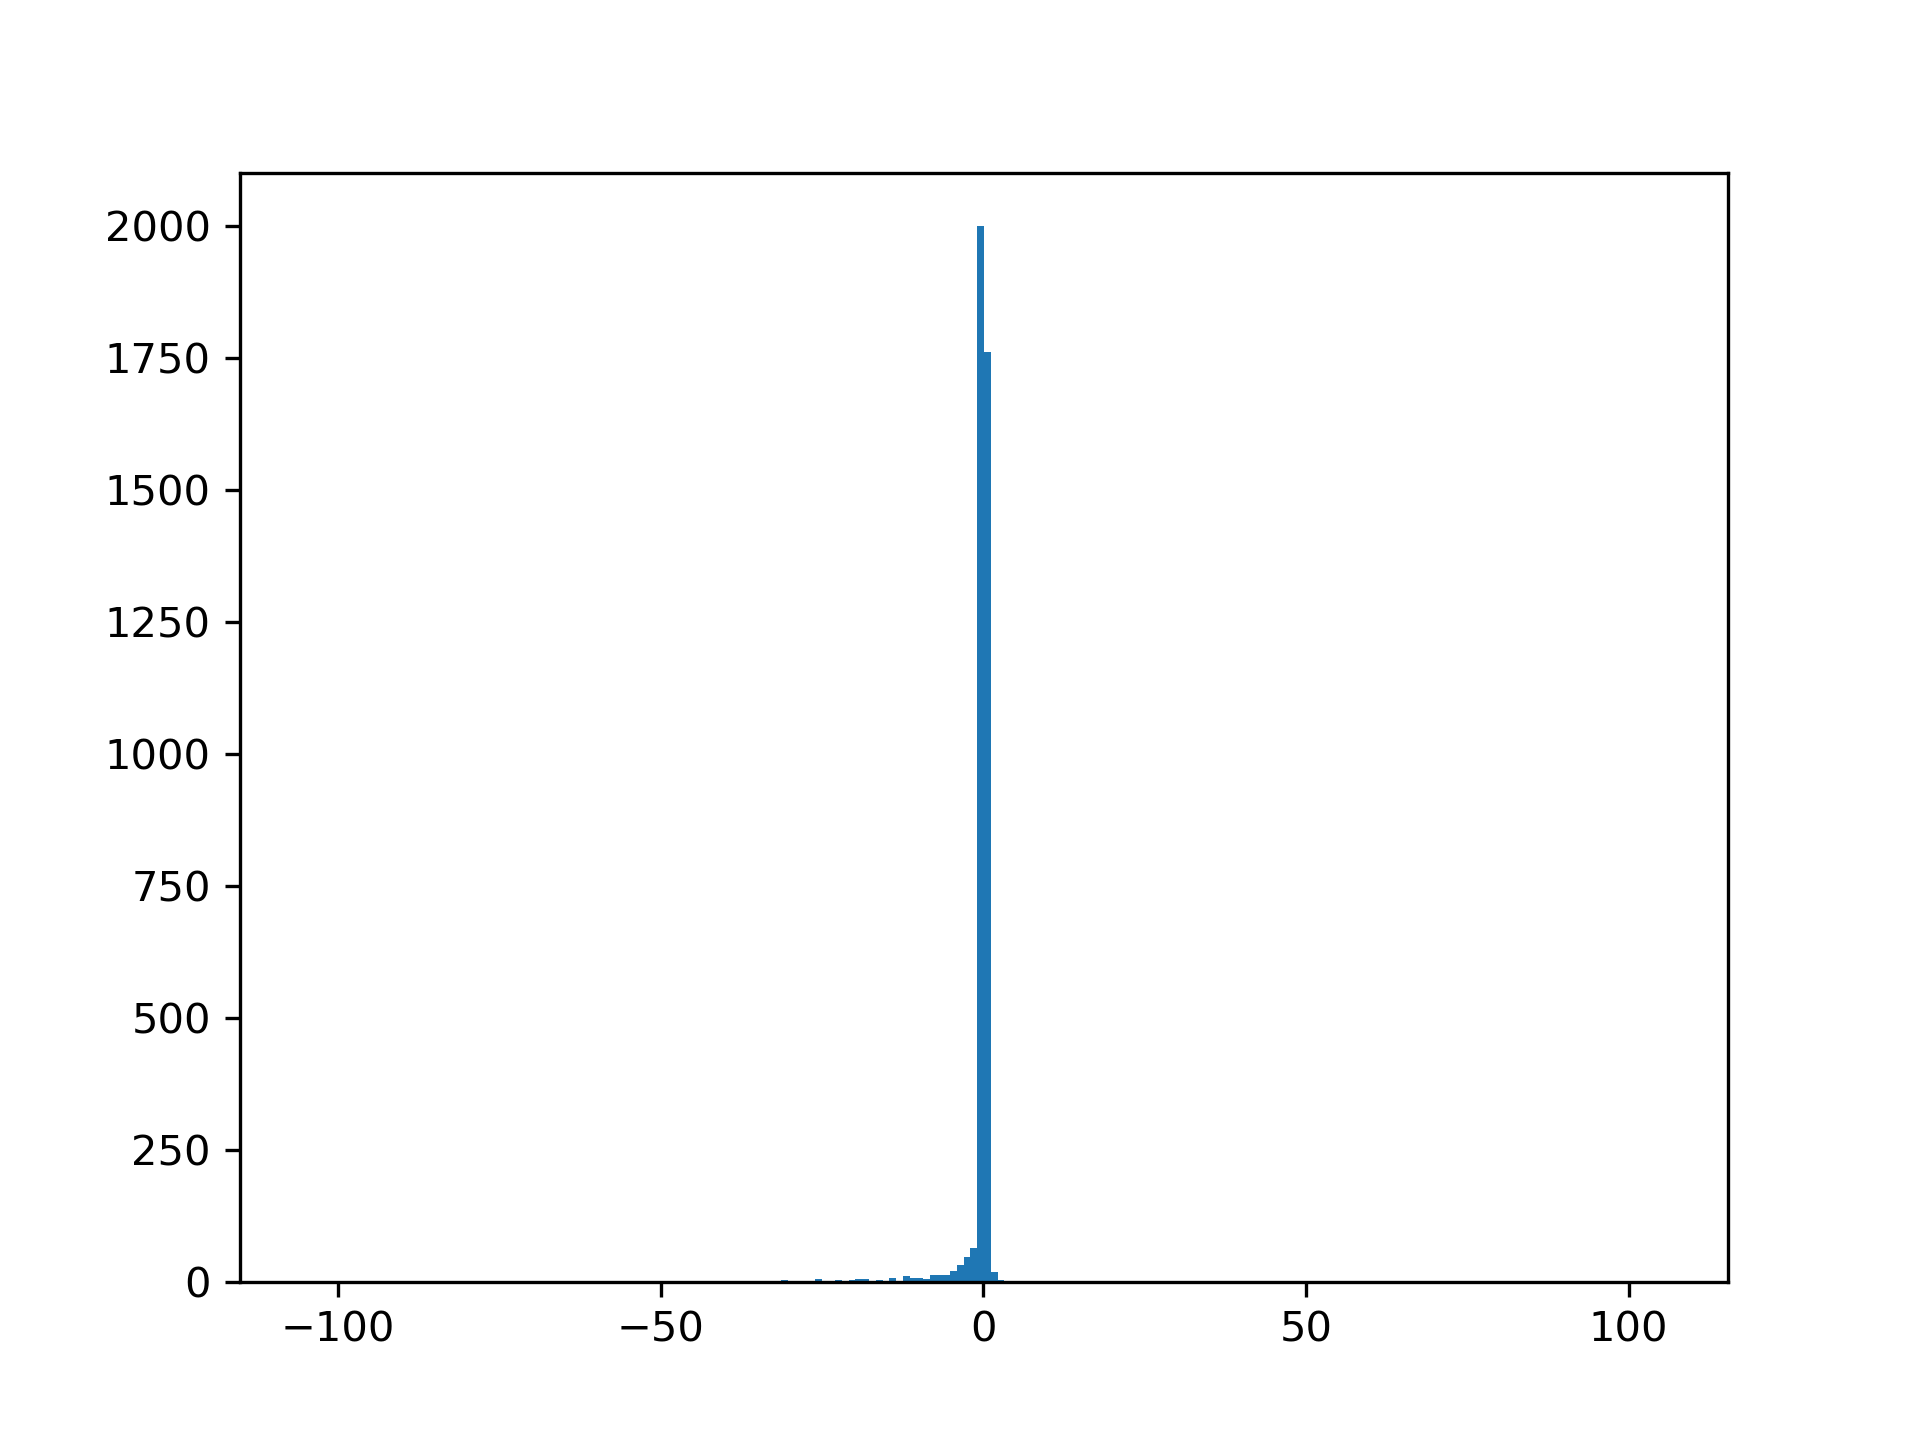
\includegraphics[width=\linewidth]{variables/EBIT Margin.png}
    \caption{Histogram EBIT Margin }
\end{figure}\section{ Profit Margin }

\begin{center}
    \begin{tabular}{|c | c|} 
    \hline
    Statystyka & Wartość \\
    \hline\hline
    Średnia arytmetyczna & -9.207095176205948 \\ 
    \hline
    Odchylenie standardowe & 177.76005721971637 \\
    \hline
    Kwartyl dolny & -0.077 \\
    \hline
    Mediana & 0.039 \\
    \hline
    Kwartyl górny & 0.13375 \\
    \hline
    Wartość najmniejsza & -8964.916 \\
    \hline
    Wartość największa & 940.041 \\
    \hline
   \end{tabular}
\end{center}

\begin{figure}[h!]
    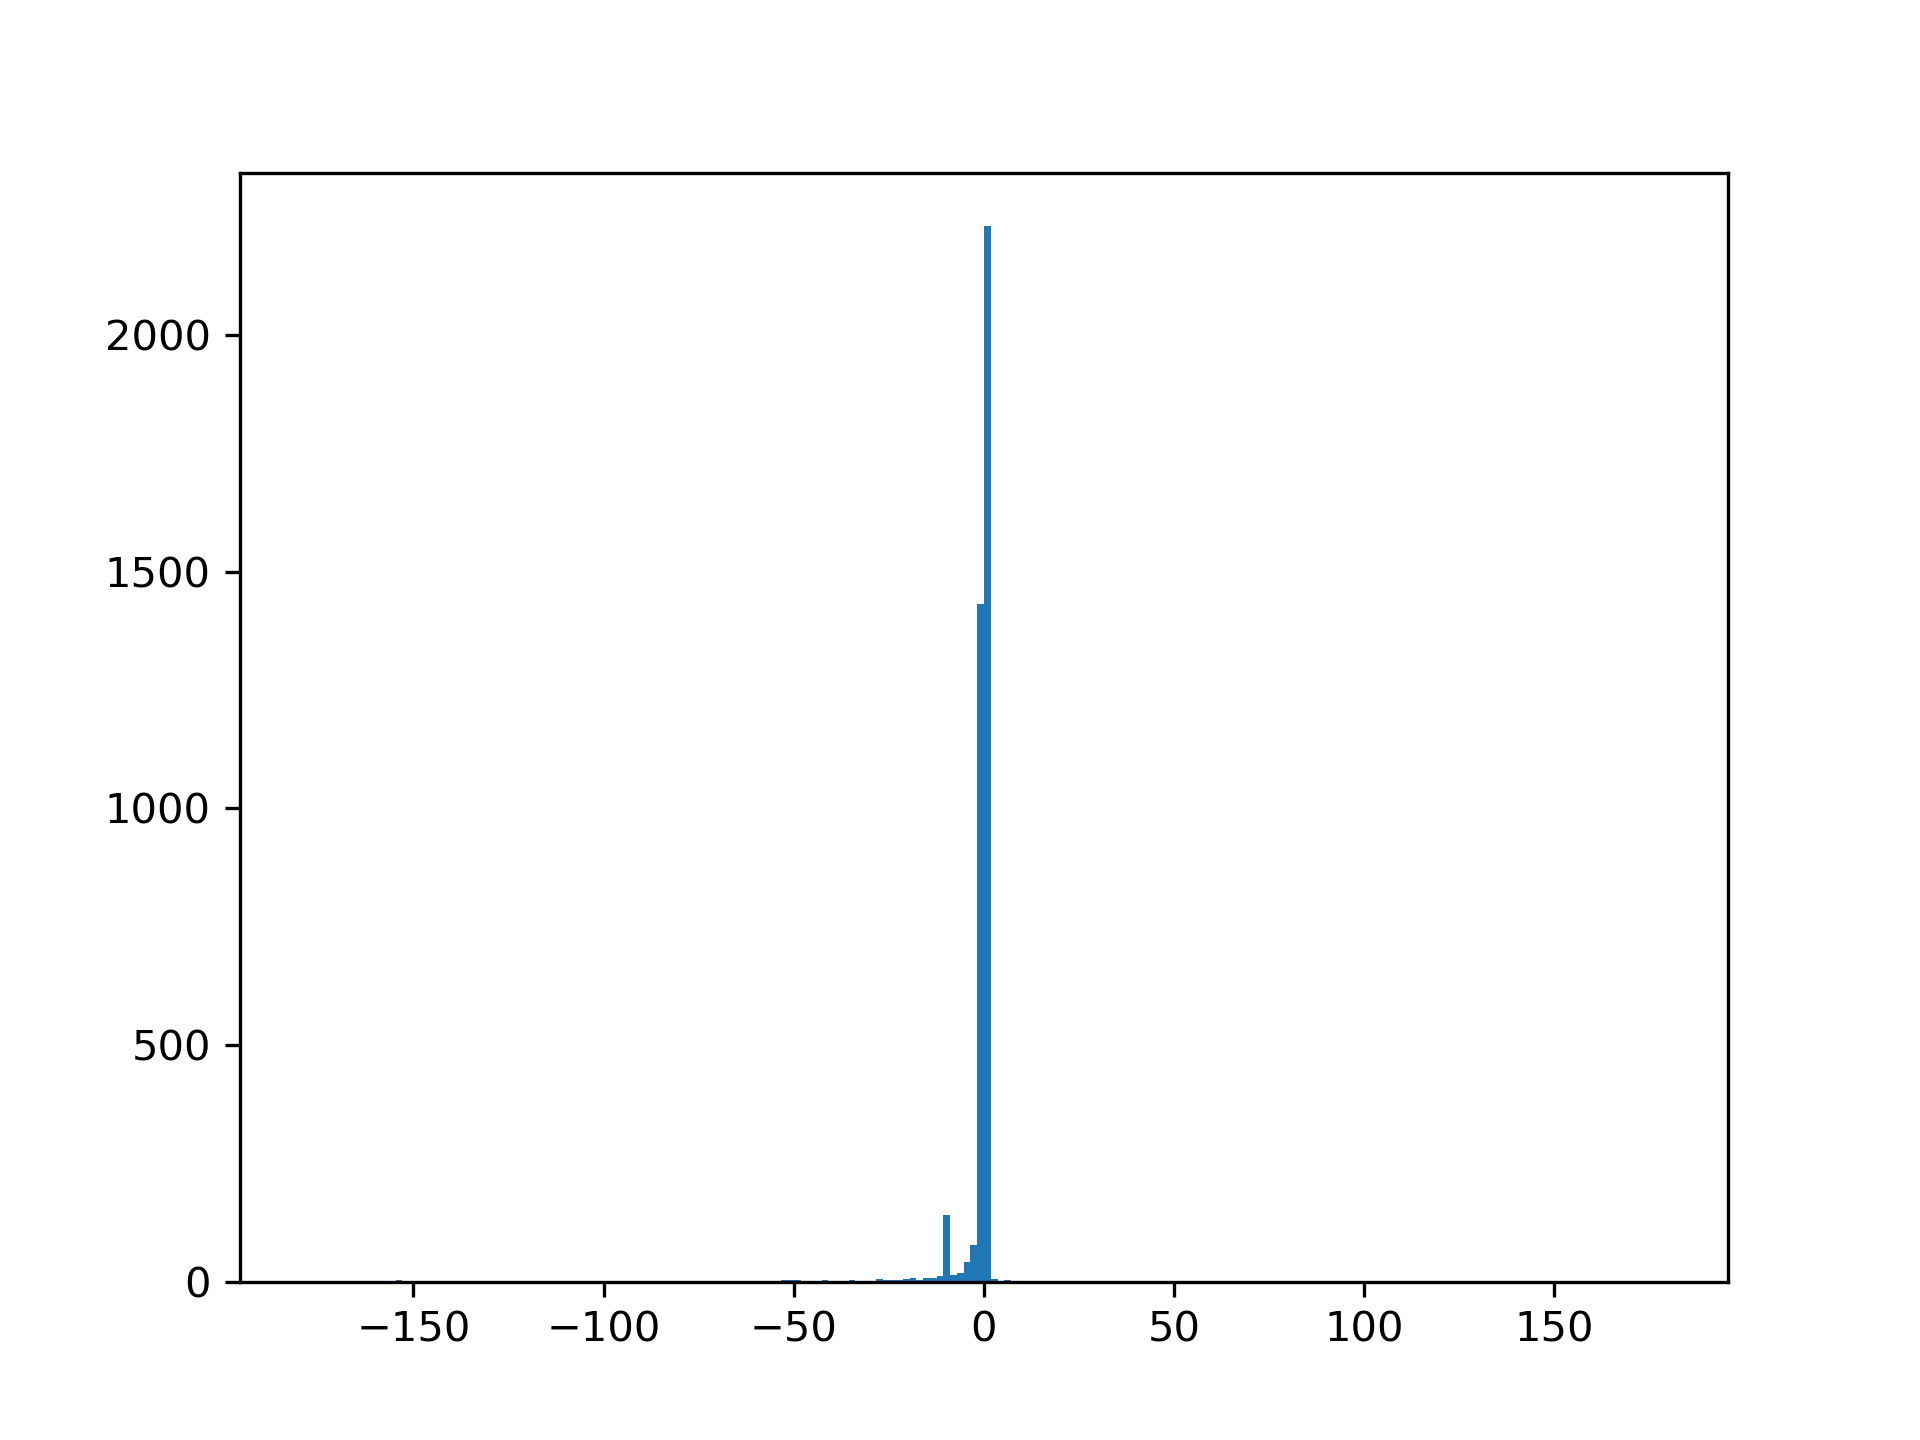
\includegraphics[width=\linewidth]{variables/Profit Margin.png}
    \caption{Histogram Profit Margin }
\end{figure}\section{ Free Cash Flow margin }

\begin{center}
    \begin{tabular}{|c | c|} 
    \hline
    Statystyka & Wartość \\
    \hline\hline
    Średnia arytmetyczna & -4.641633988355168 \\ 
    \hline
    Odchylenie standardowe & 95.19911309785644 \\
    \hline
    Kwartyl dolny & -0.039474999999999996 \\
    \hline
    Mediana & 0.0458 \\
    \hline
    Kwartyl górny & 0.16325 \\
    \hline
    Wartość najmniejsza & -4821.5 \\
    \hline
    Wartość największa & 244.6356 \\
    \hline
   \end{tabular}
\end{center}

\begin{figure}[h!]
    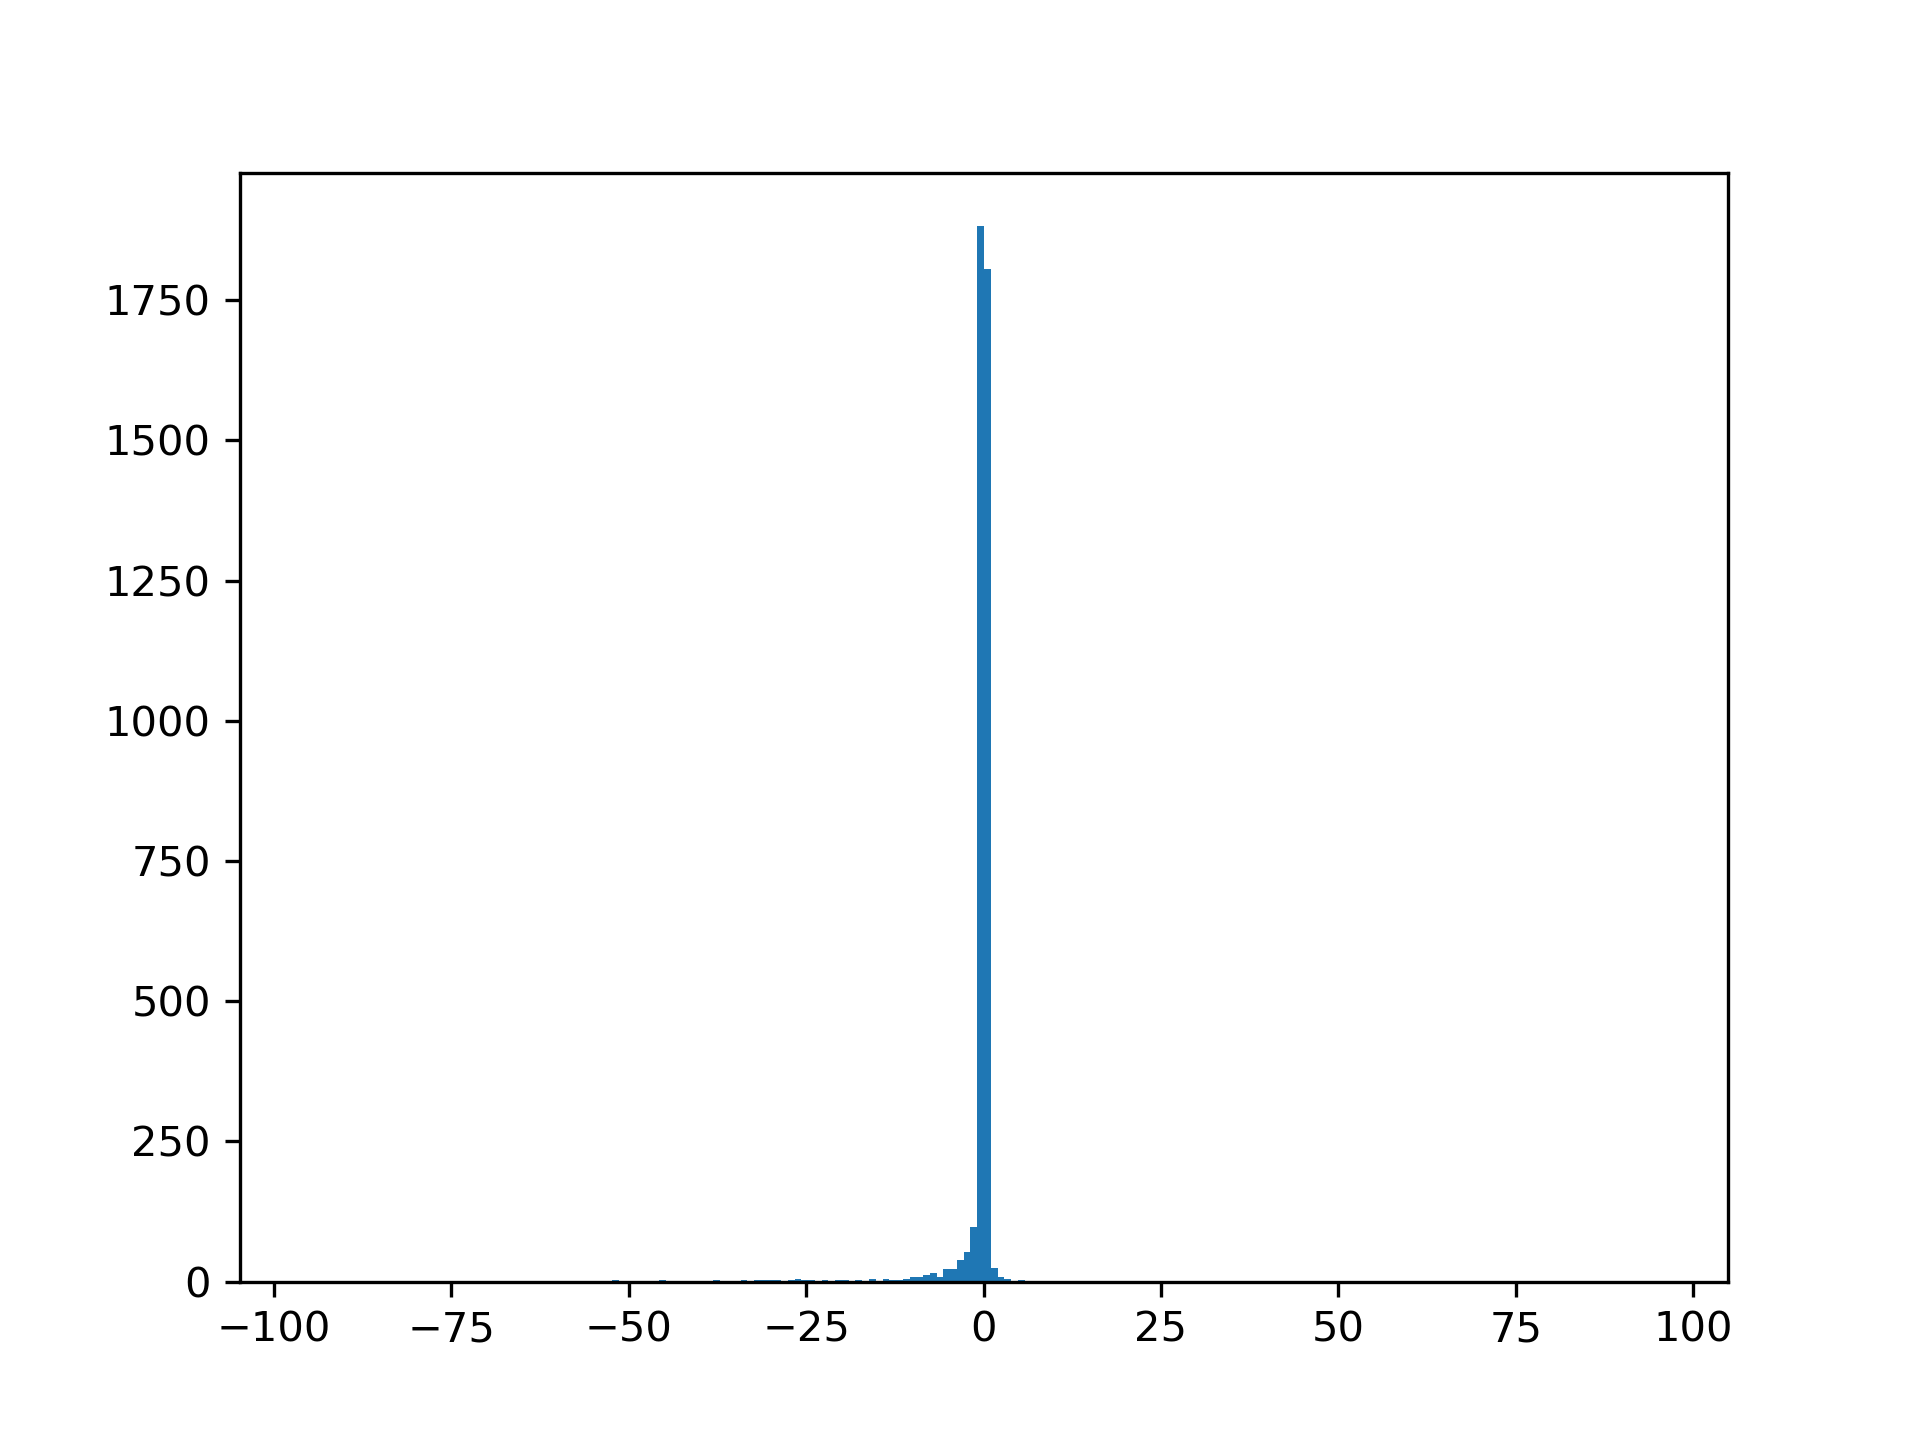
\includegraphics[width=\linewidth]{variables/Free Cash Flow margin.png}
    \caption{Histogram Free Cash Flow margin }
\end{figure}\section{ EBITDA }

\begin{center}
    \begin{tabular}{|c | c|} 
    \hline
    Statystyka & Wartość \\
    \hline\hline
    Średnia arytmetyczna & 959935183.8215535 \\ 
    \hline
    Odchylenie standardowe & 3765268429.9602165 \\
    \hline
    Kwartyl dolny & 1579250.0 \\
    \hline
    Mediana & 85310500.0 \\
    \hline
    Kwartyl górny & 477463250.0 \\
    \hline
    Wartość najmniejsza & -8992000000.0 \\
    \hline
    Wartość największa & 83806000000.0 \\
    \hline
   \end{tabular}
\end{center}

\begin{figure}[h!]
    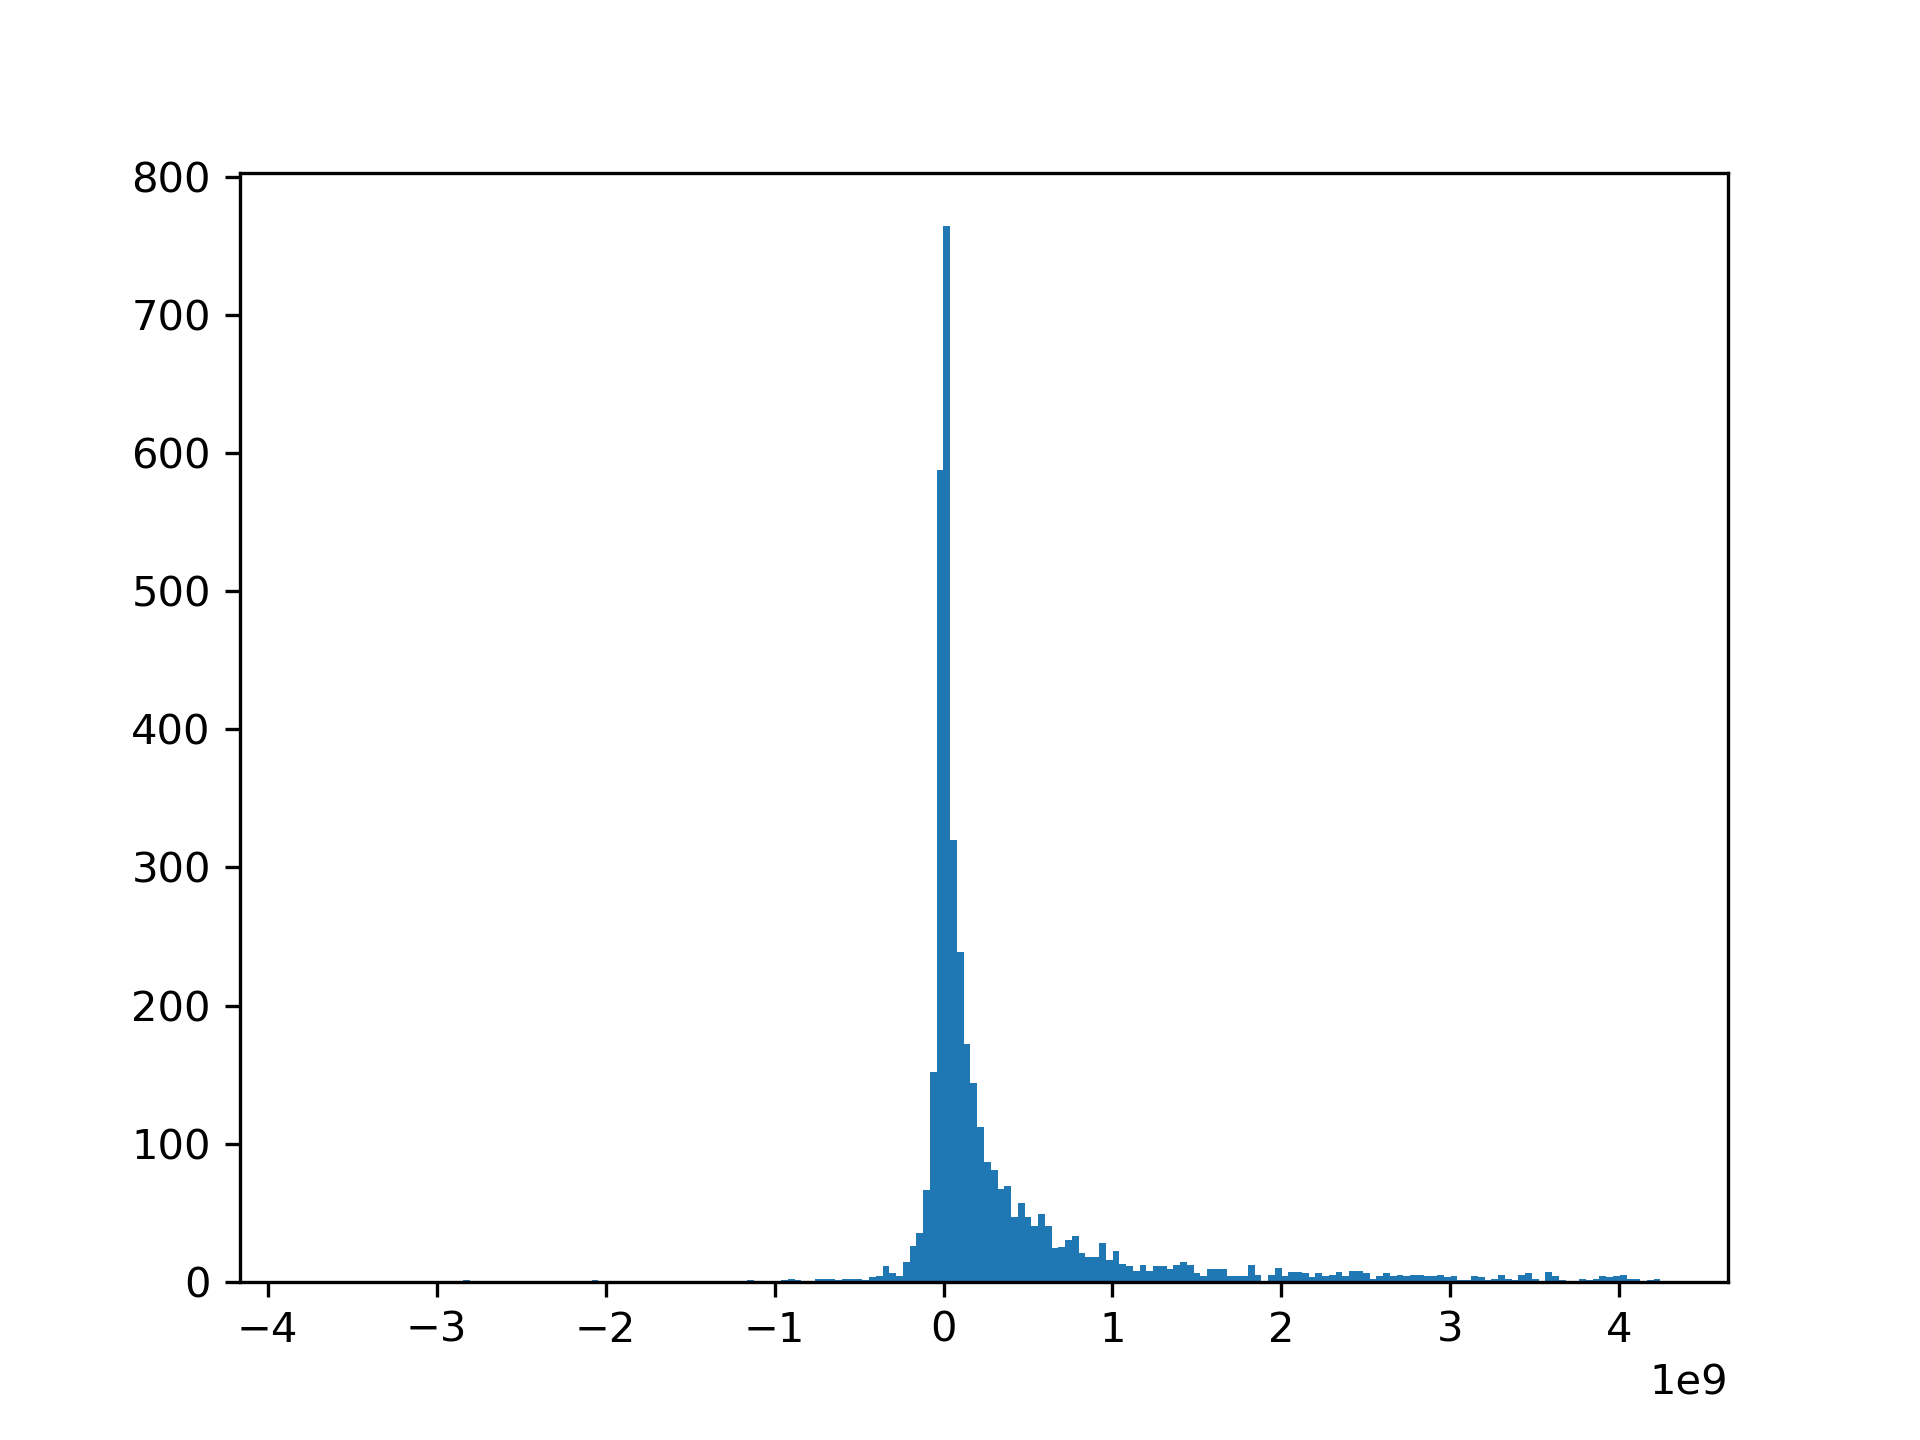
\includegraphics[width=\linewidth]{variables/EBITDA.png}
    \caption{Histogram EBITDA }
\end{figure}\section{ EBIT }

\begin{center}
    \begin{tabular}{|c | c|} 
    \hline
    Statystyka & Wartość \\
    \hline\hline
    Średnia arytmetyczna & 659108769.6742082 \\ 
    \hline
    Odchylenie standardowe & 2735969862.103594 \\
    \hline
    Kwartyl dolny & -3954380.0 \\
    \hline
    Mediana & 48079000.0 \\
    \hline
    Kwartyl górny & 307882000.0 \\
    \hline
    Wartość najmniejsza & -16713000000.0 \\
    \hline
    Wartość największa & 72903000000.0 \\
    \hline
   \end{tabular}
\end{center}

\begin{figure}[h!]
    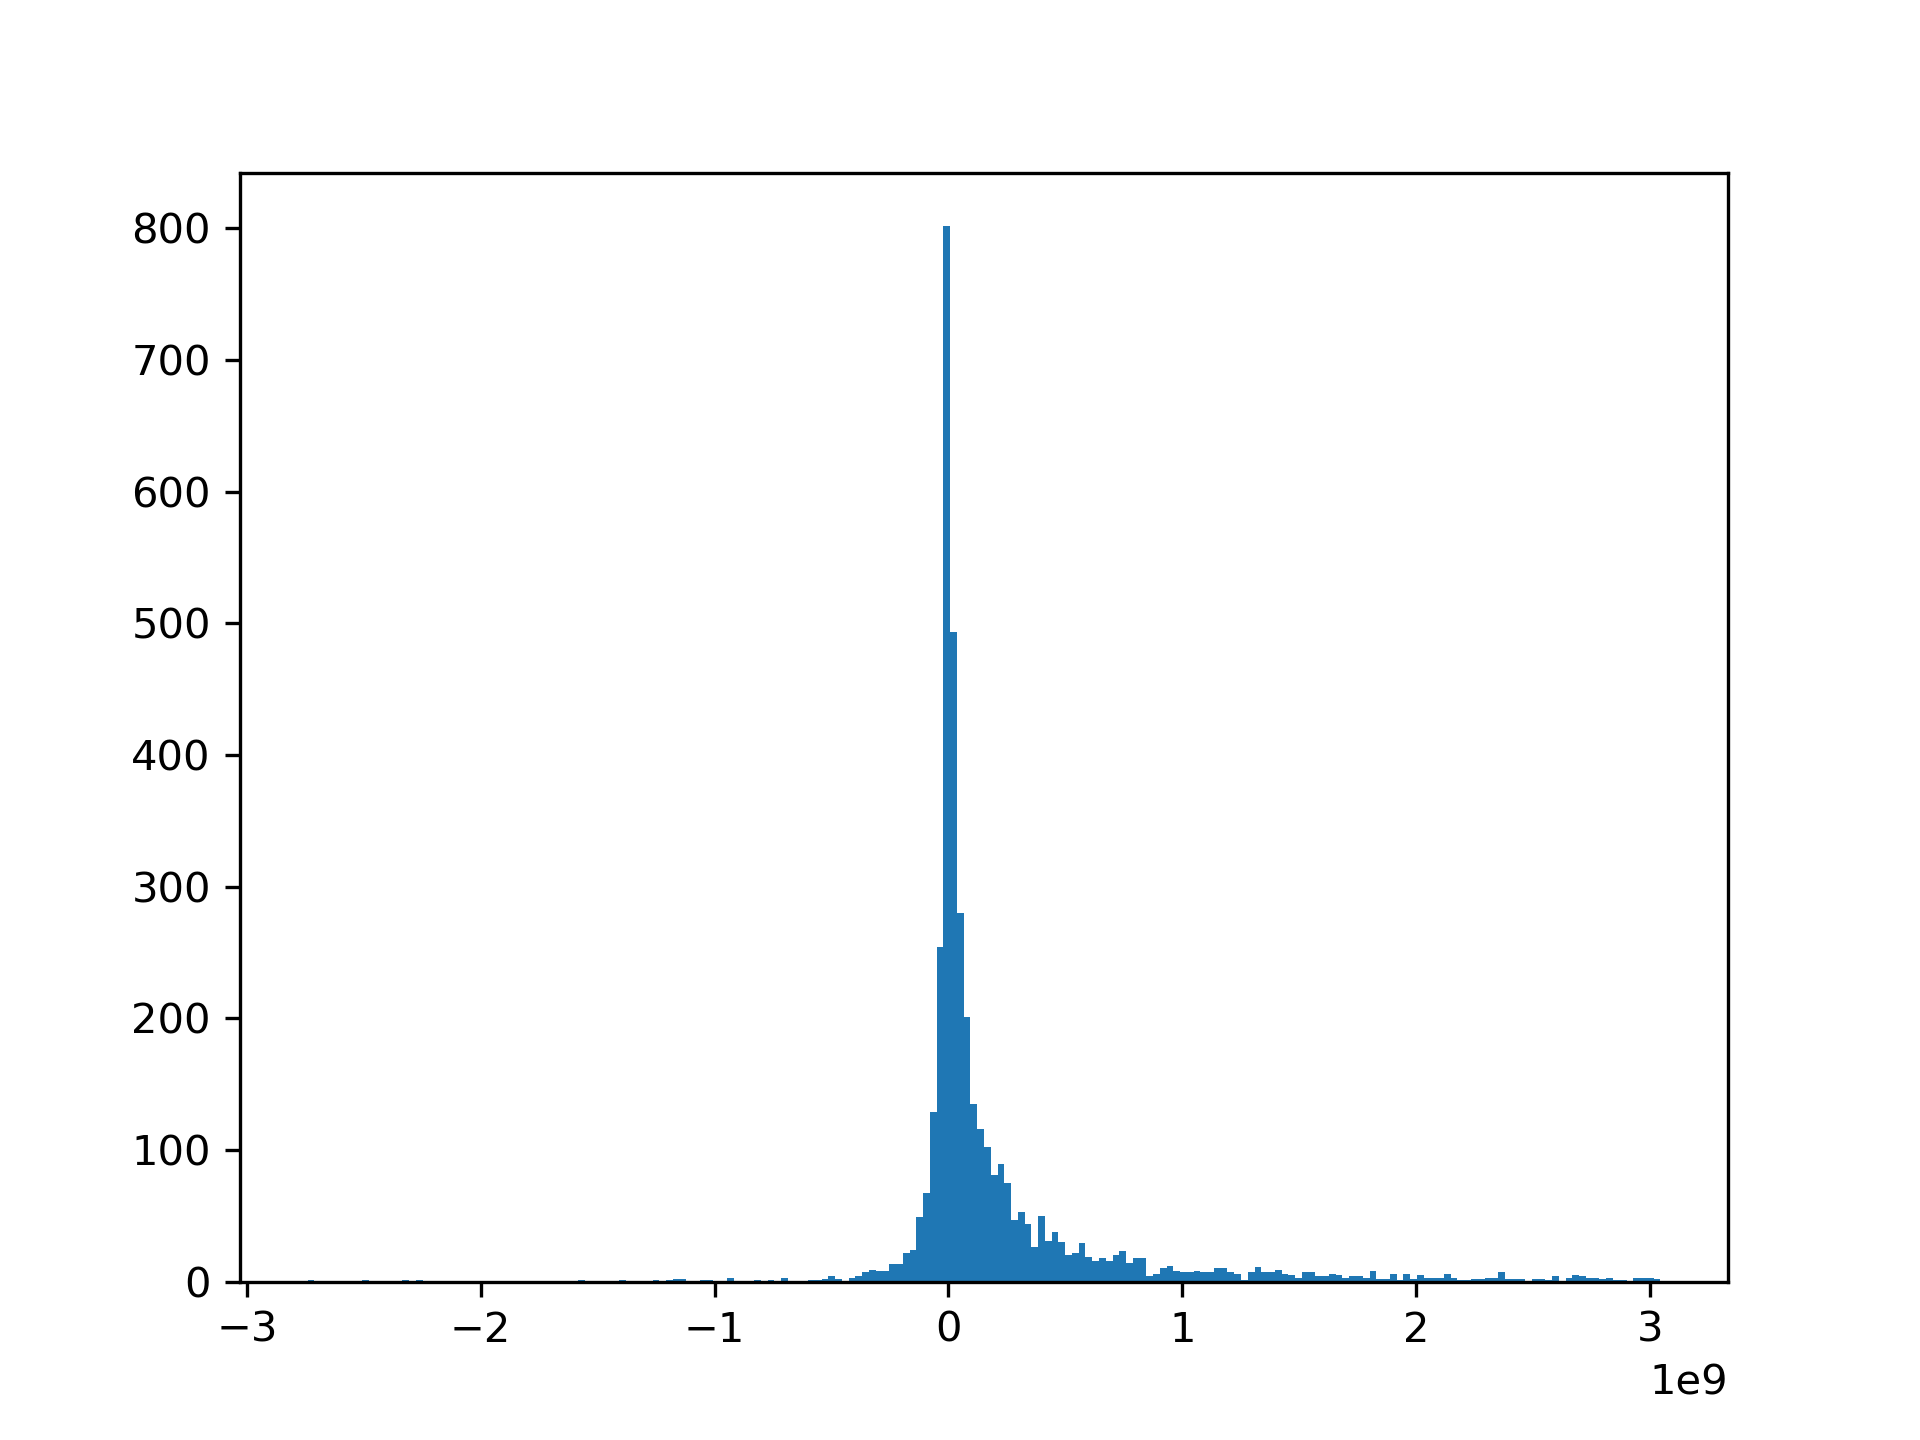
\includegraphics[width=\linewidth]{variables/EBIT.png}
    \caption{Histogram EBIT }
\end{figure}\section{ Consolidated Income }

\begin{center}
    \begin{tabular}{|c | c|} 
    \hline
    Statystyka & Wartość \\
    \hline\hline
    Średnia arytmetyczna & 451725958.08517635 \\ 
    \hline
    Odchylenie standardowe & 2108059447.5614533 \\
    \hline
    Kwartyl dolny & -10798127.25 \\
    \hline
    Mediana & 24951500.0 \\
    \hline
    Kwartyl górny & 205455750.0 \\
    \hline
    Wartość najmniejsza & -22443000000.0 \\
    \hline
    Wartość największa & 59531000000.0 \\
    \hline
   \end{tabular}
\end{center}

\begin{figure}[h!]
    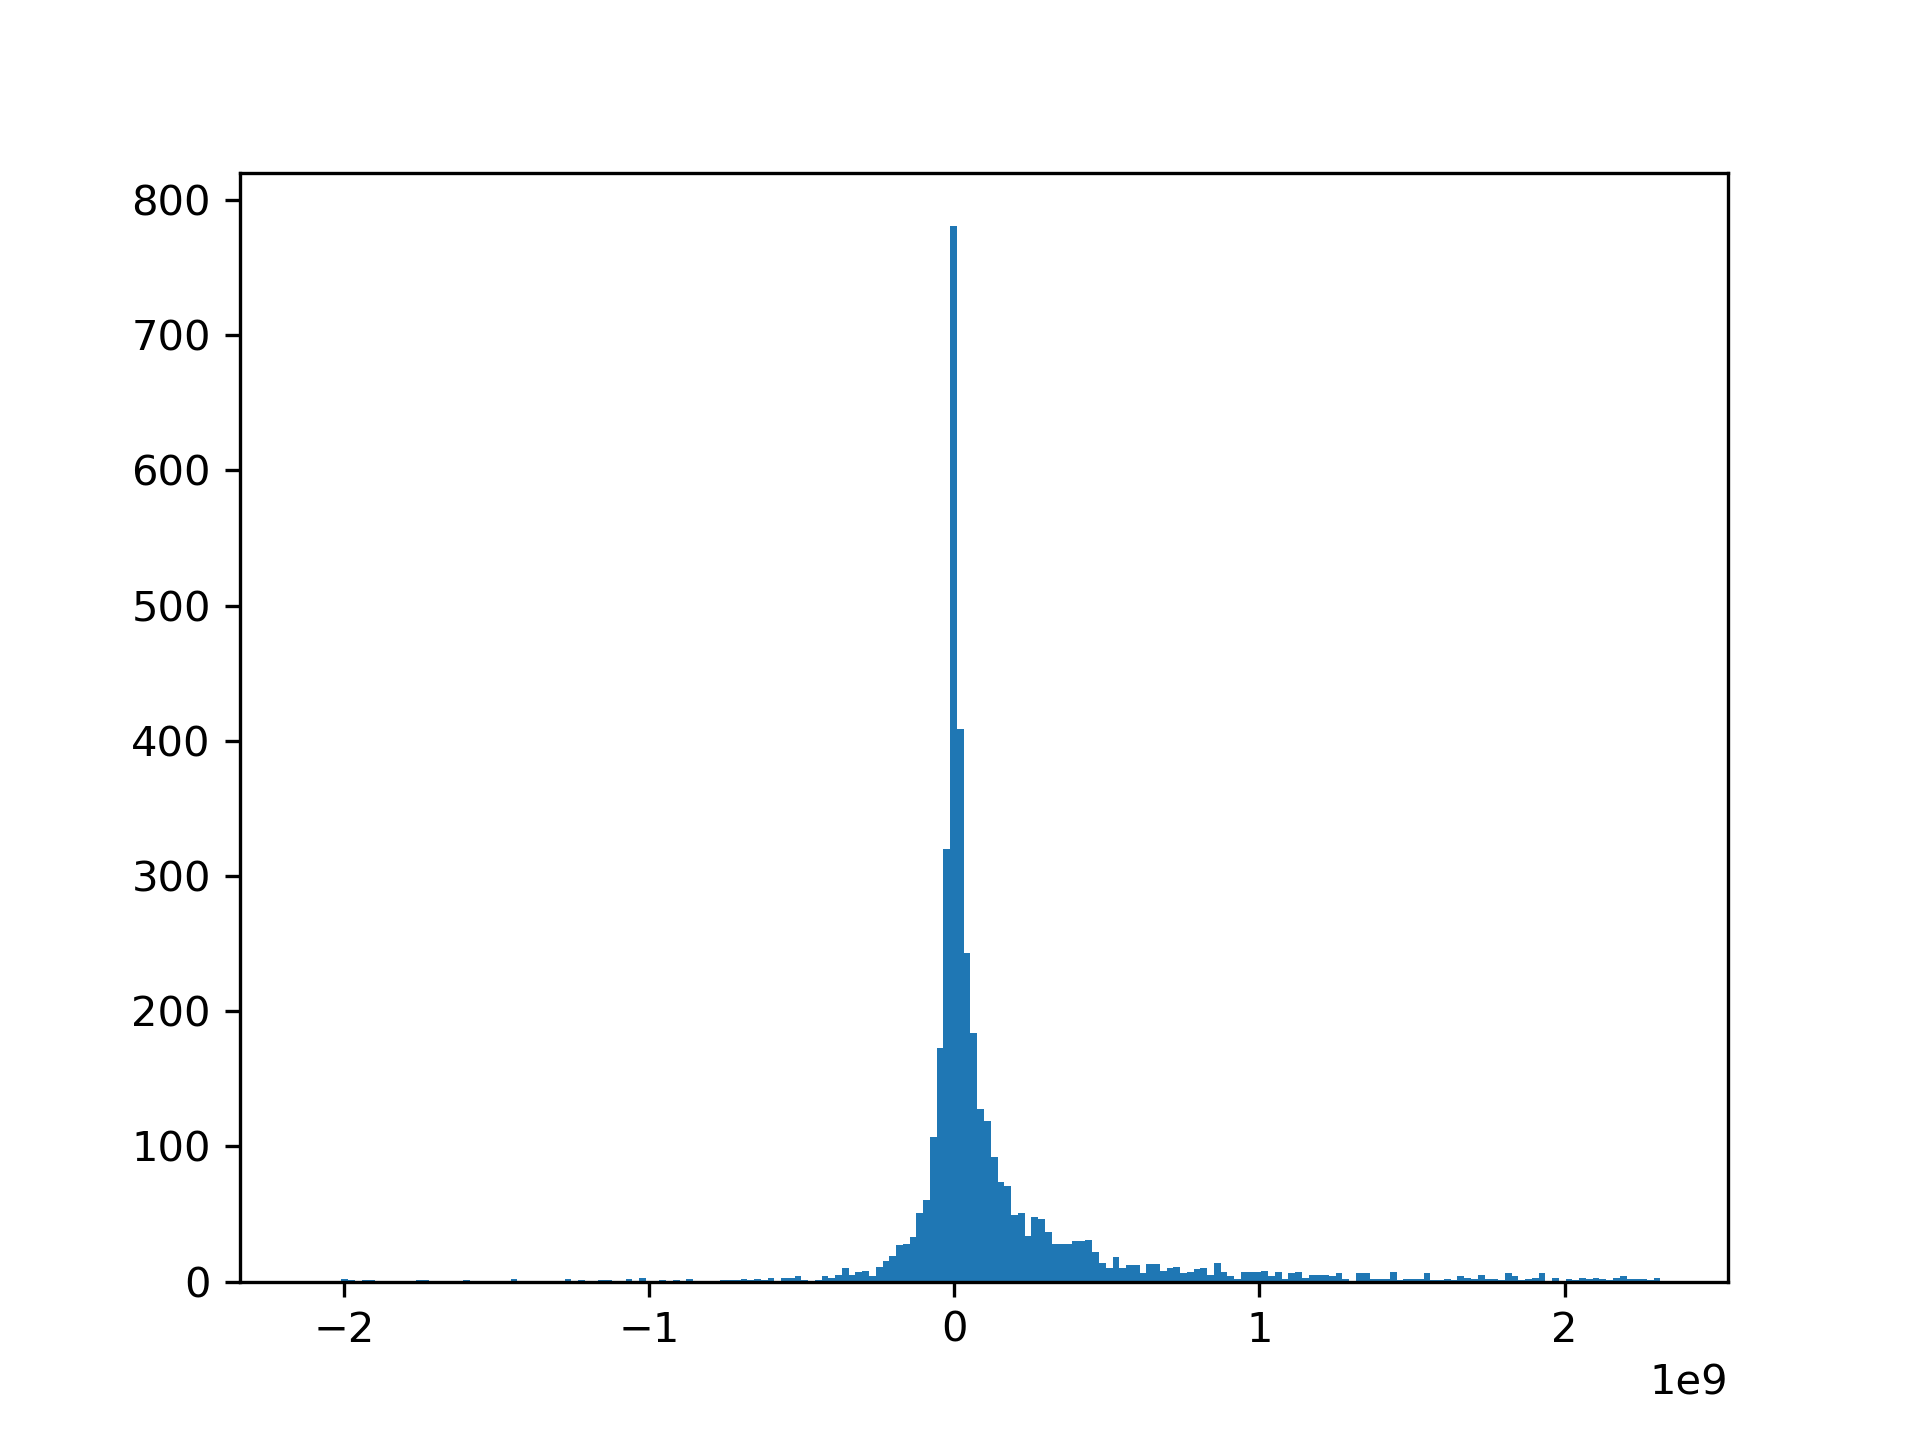
\includegraphics[width=\linewidth]{variables/Consolidated Income.png}
    \caption{Histogram Consolidated Income }
\end{figure}\section{ Earnings Before Tax Margin }

\begin{center}
    \begin{tabular}{|c | c|} 
    \hline
    Statystyka & Wartość \\
    \hline\hline
    Średnia arytmetyczna & -4.938629524502669 \\ 
    \hline
    Odchylenie standardowe & 104.69455088345339 \\
    \hline
    Kwartyl dolny & -0.029525 \\
    \hline
    Mediana & 0.058550000000000005 \\
    \hline
    Kwartyl górny & 0.1738 \\
    \hline
    Wartość najmniejsza & -5009.1667 \\
    \hline
    Wartość największa & 1056.4658 \\
    \hline
   \end{tabular}
\end{center}

\begin{figure}[h!]
    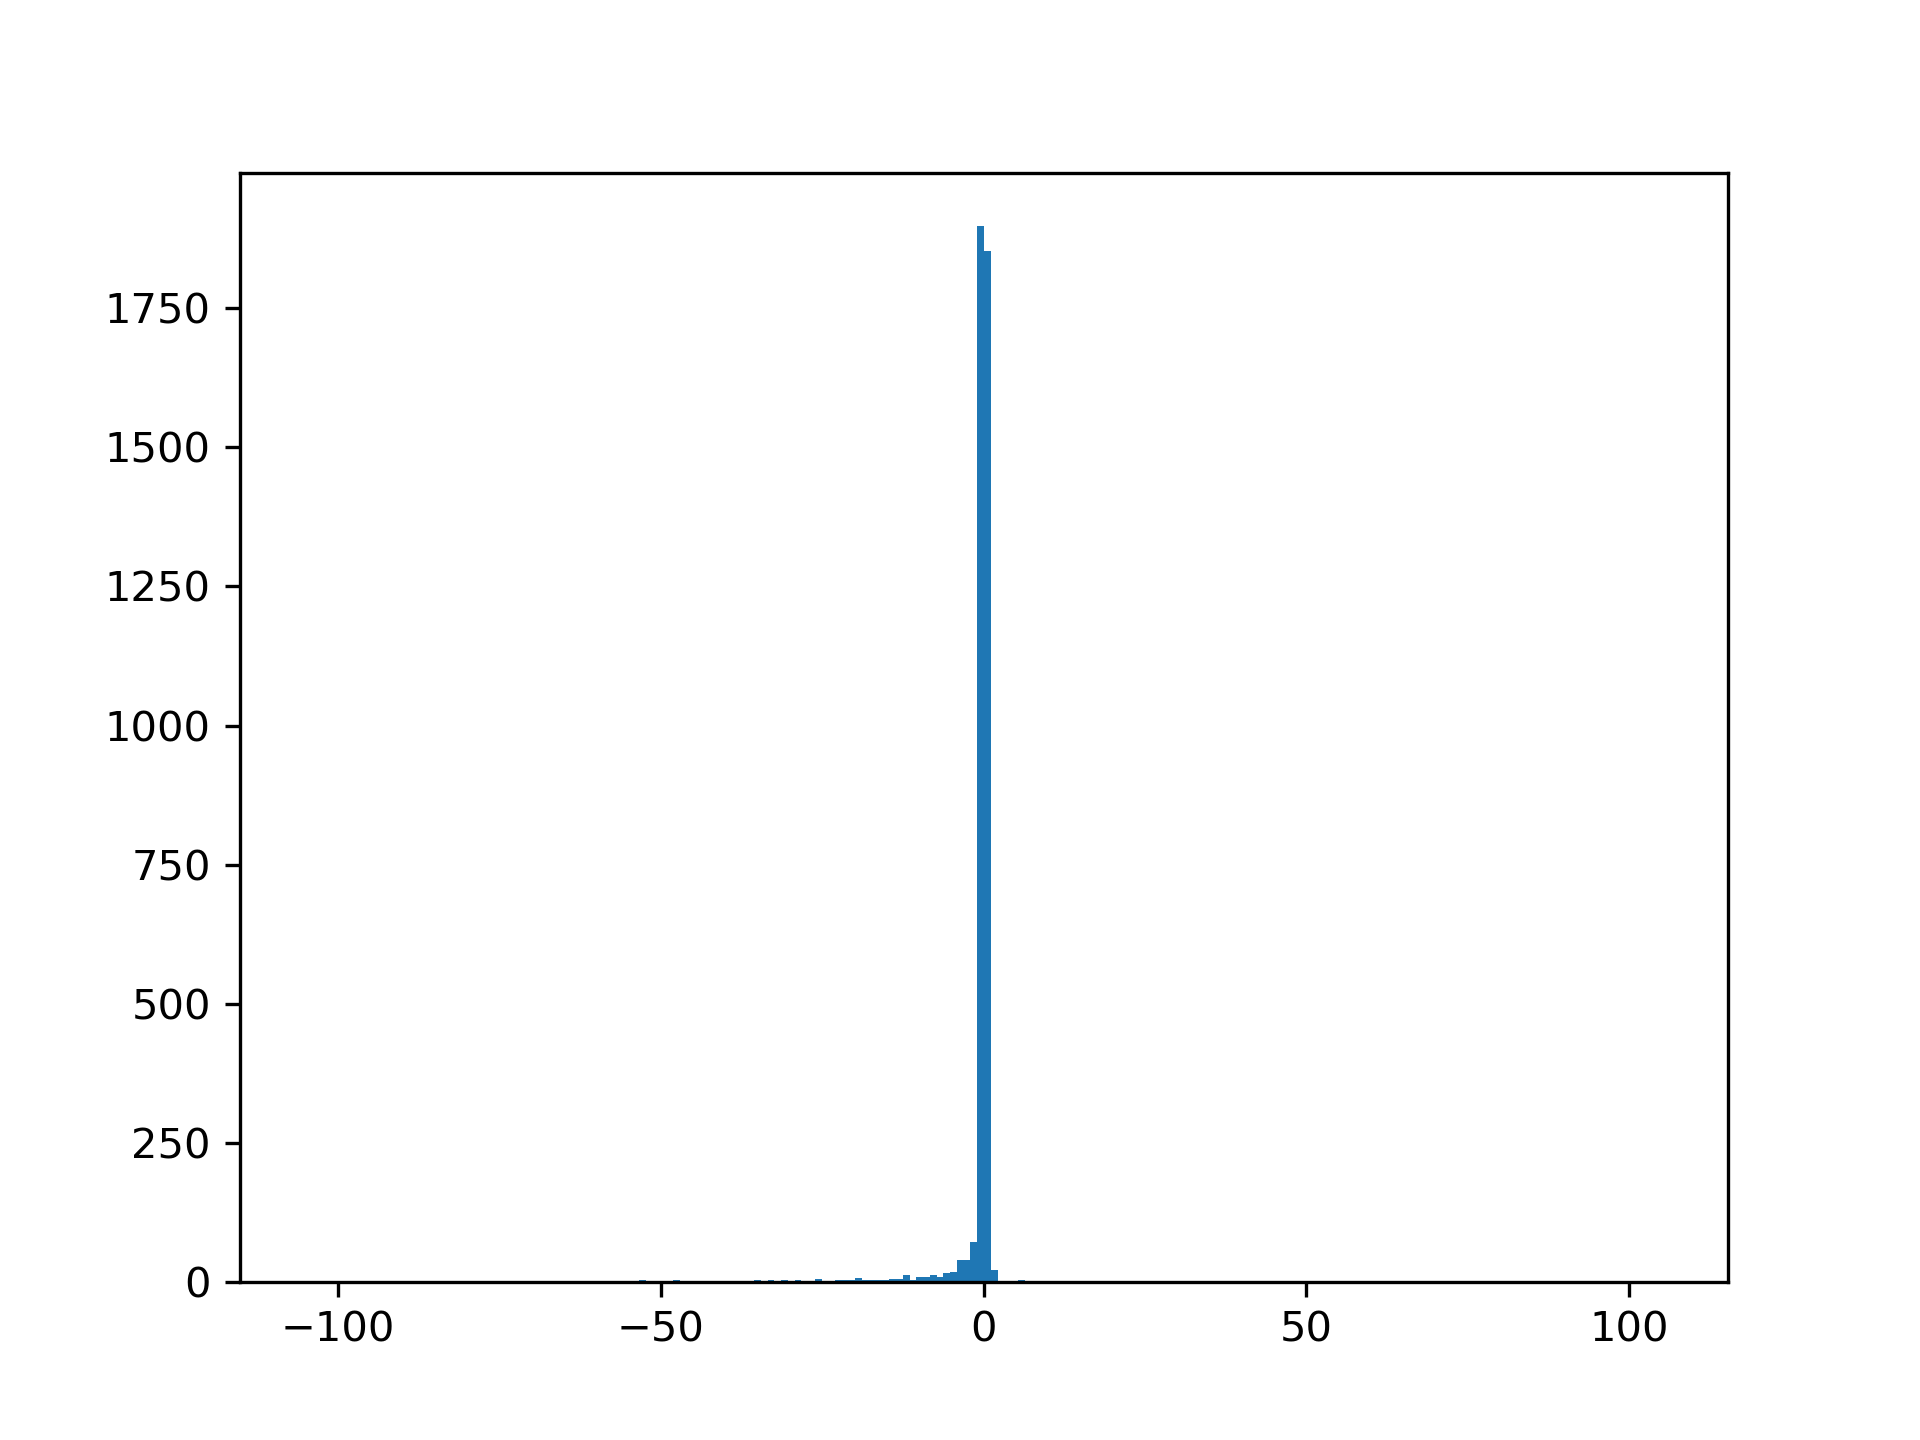
\includegraphics[width=\linewidth]{variables/Earnings Before Tax Margin.png}
    \caption{Histogram Earnings Before Tax Margin }
\end{figure}\section{ Net Profit Margin }

\begin{center}
    \begin{tabular}{|c | c|} 
    \hline
    Statystyka & Wartość \\
    \hline\hline
    Średnia arytmetyczna & -4.934547876728949 \\ 
    \hline
    Odchylenie standardowe & 104.64891458502912 \\
    \hline
    Kwartyl dolny & -0.029575 \\
    \hline
    Mediana & 0.0462 \\
    \hline
    Kwartyl górny & 0.145975 \\
    \hline
    Wartość najmniejsza & -5009.1667 \\
    \hline
    Wartość największa & 1056.4658 \\
    \hline
   \end{tabular}
\end{center}

\begin{figure}[h!]
    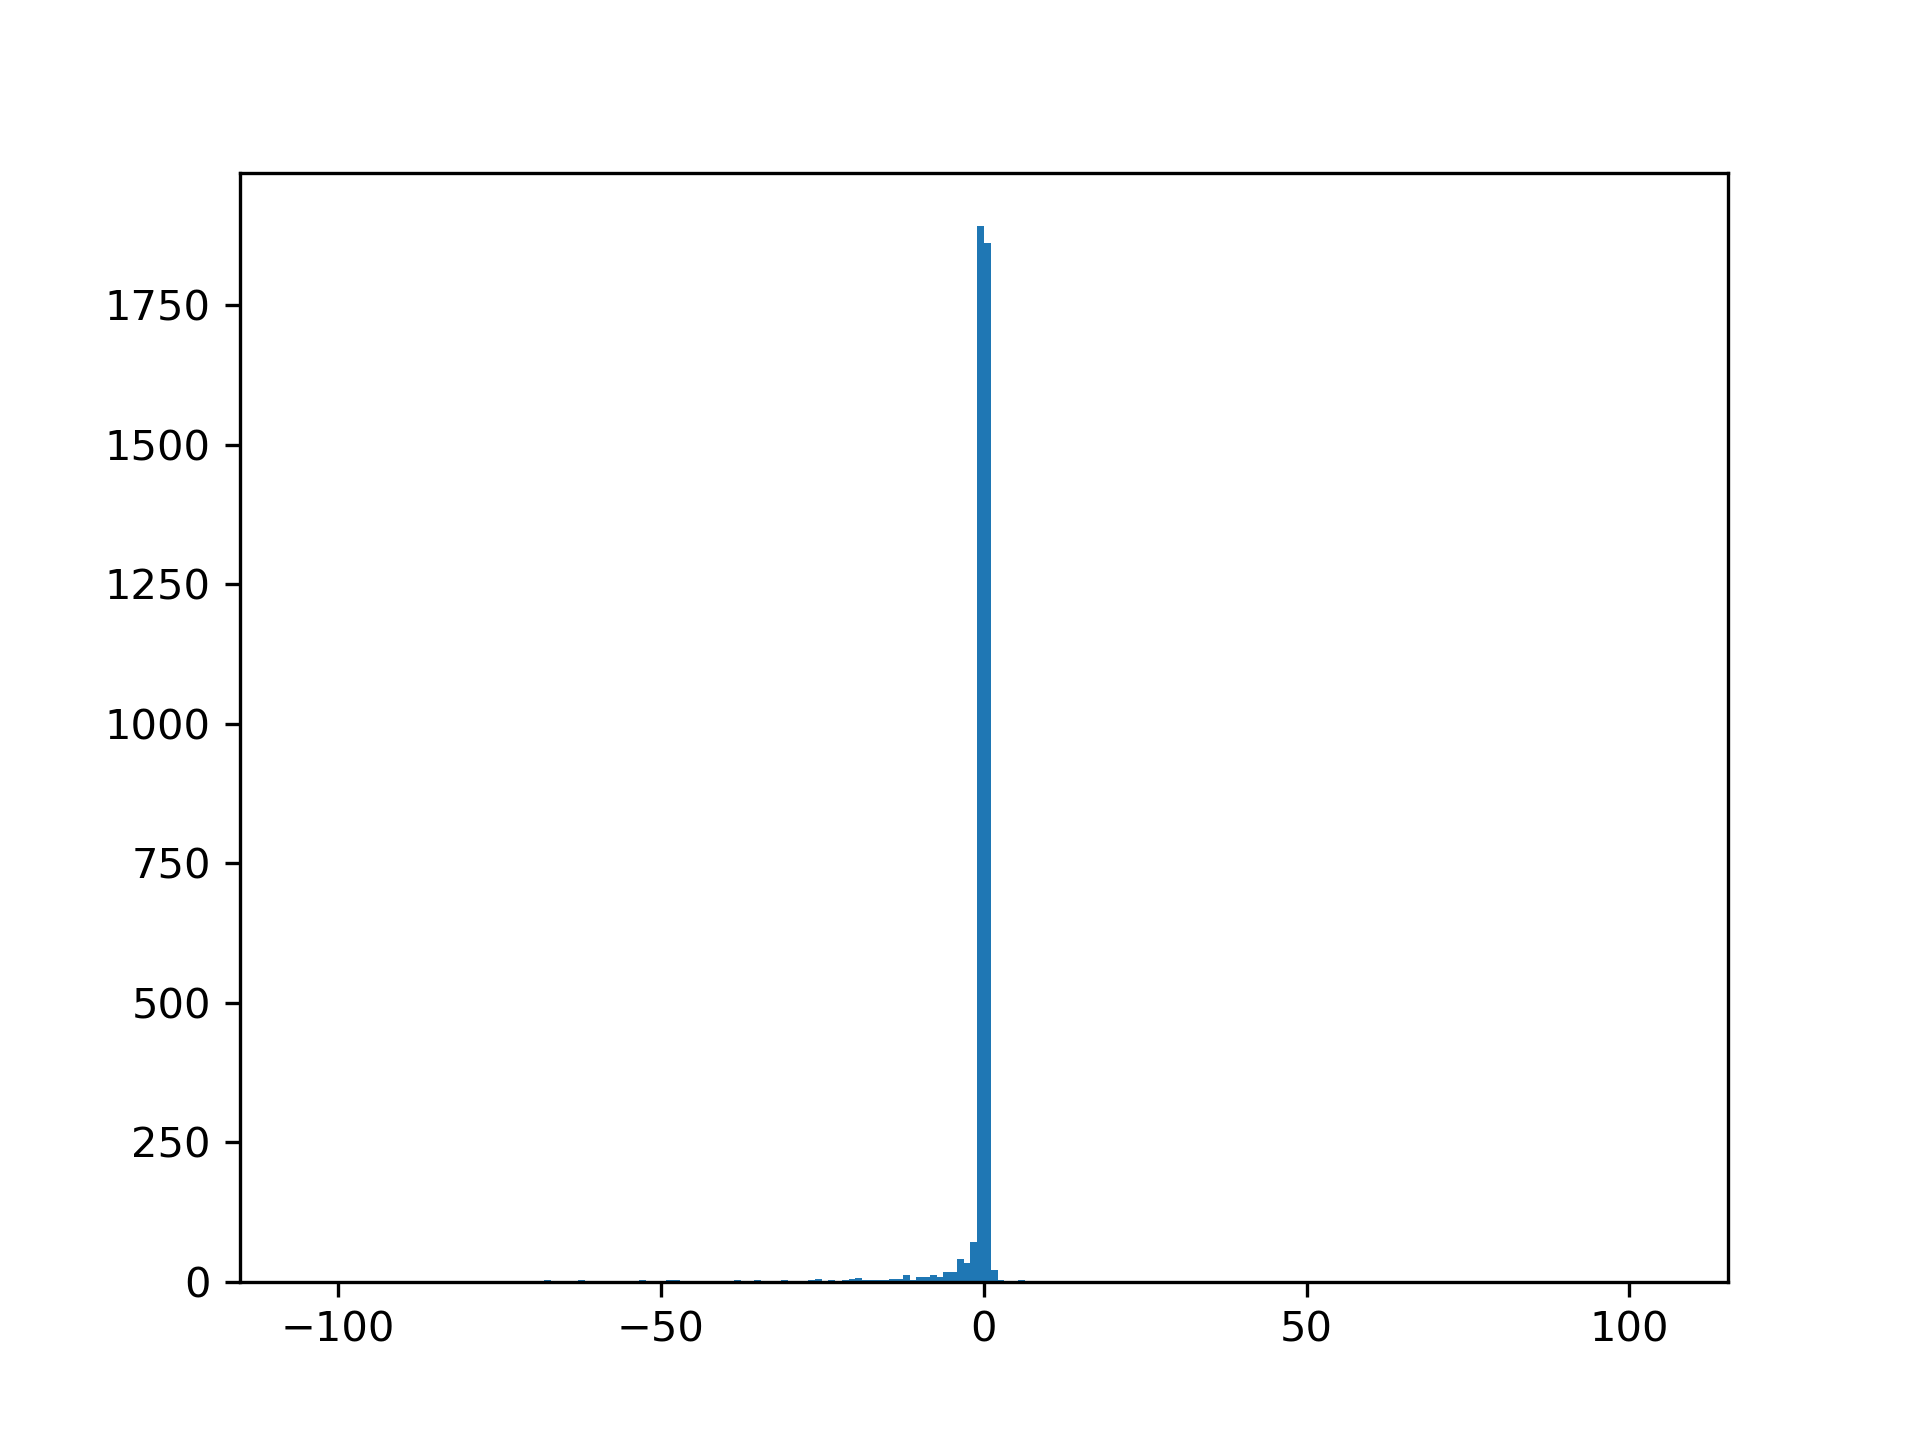
\includegraphics[width=\linewidth]{variables/Net Profit Margin.png}
    \caption{Histogram Net Profit Margin }
\end{figure}\section{ Cash and cash equivalents }

\begin{center}
    \begin{tabular}{|c | c|} 
    \hline
    Statystyka & Wartość \\
    \hline\hline
    Średnia arytmetyczna & 1575257370.328684 \\ 
    \hline
    Odchylenie standardowe & 15859977285.192768 \\
    \hline
    Kwartyl dolny & 18612250.0 \\
    \hline
    Mediana & 78211500.0 \\
    \hline
    Kwartyl górny & 314804861.1111 \\
    \hline
    Wartość najmniejsza & 0.0 \\
    \hline
    Wartość największa & 494891265176.166 \\
    \hline
   \end{tabular}
\end{center}

\begin{figure}[h!]
    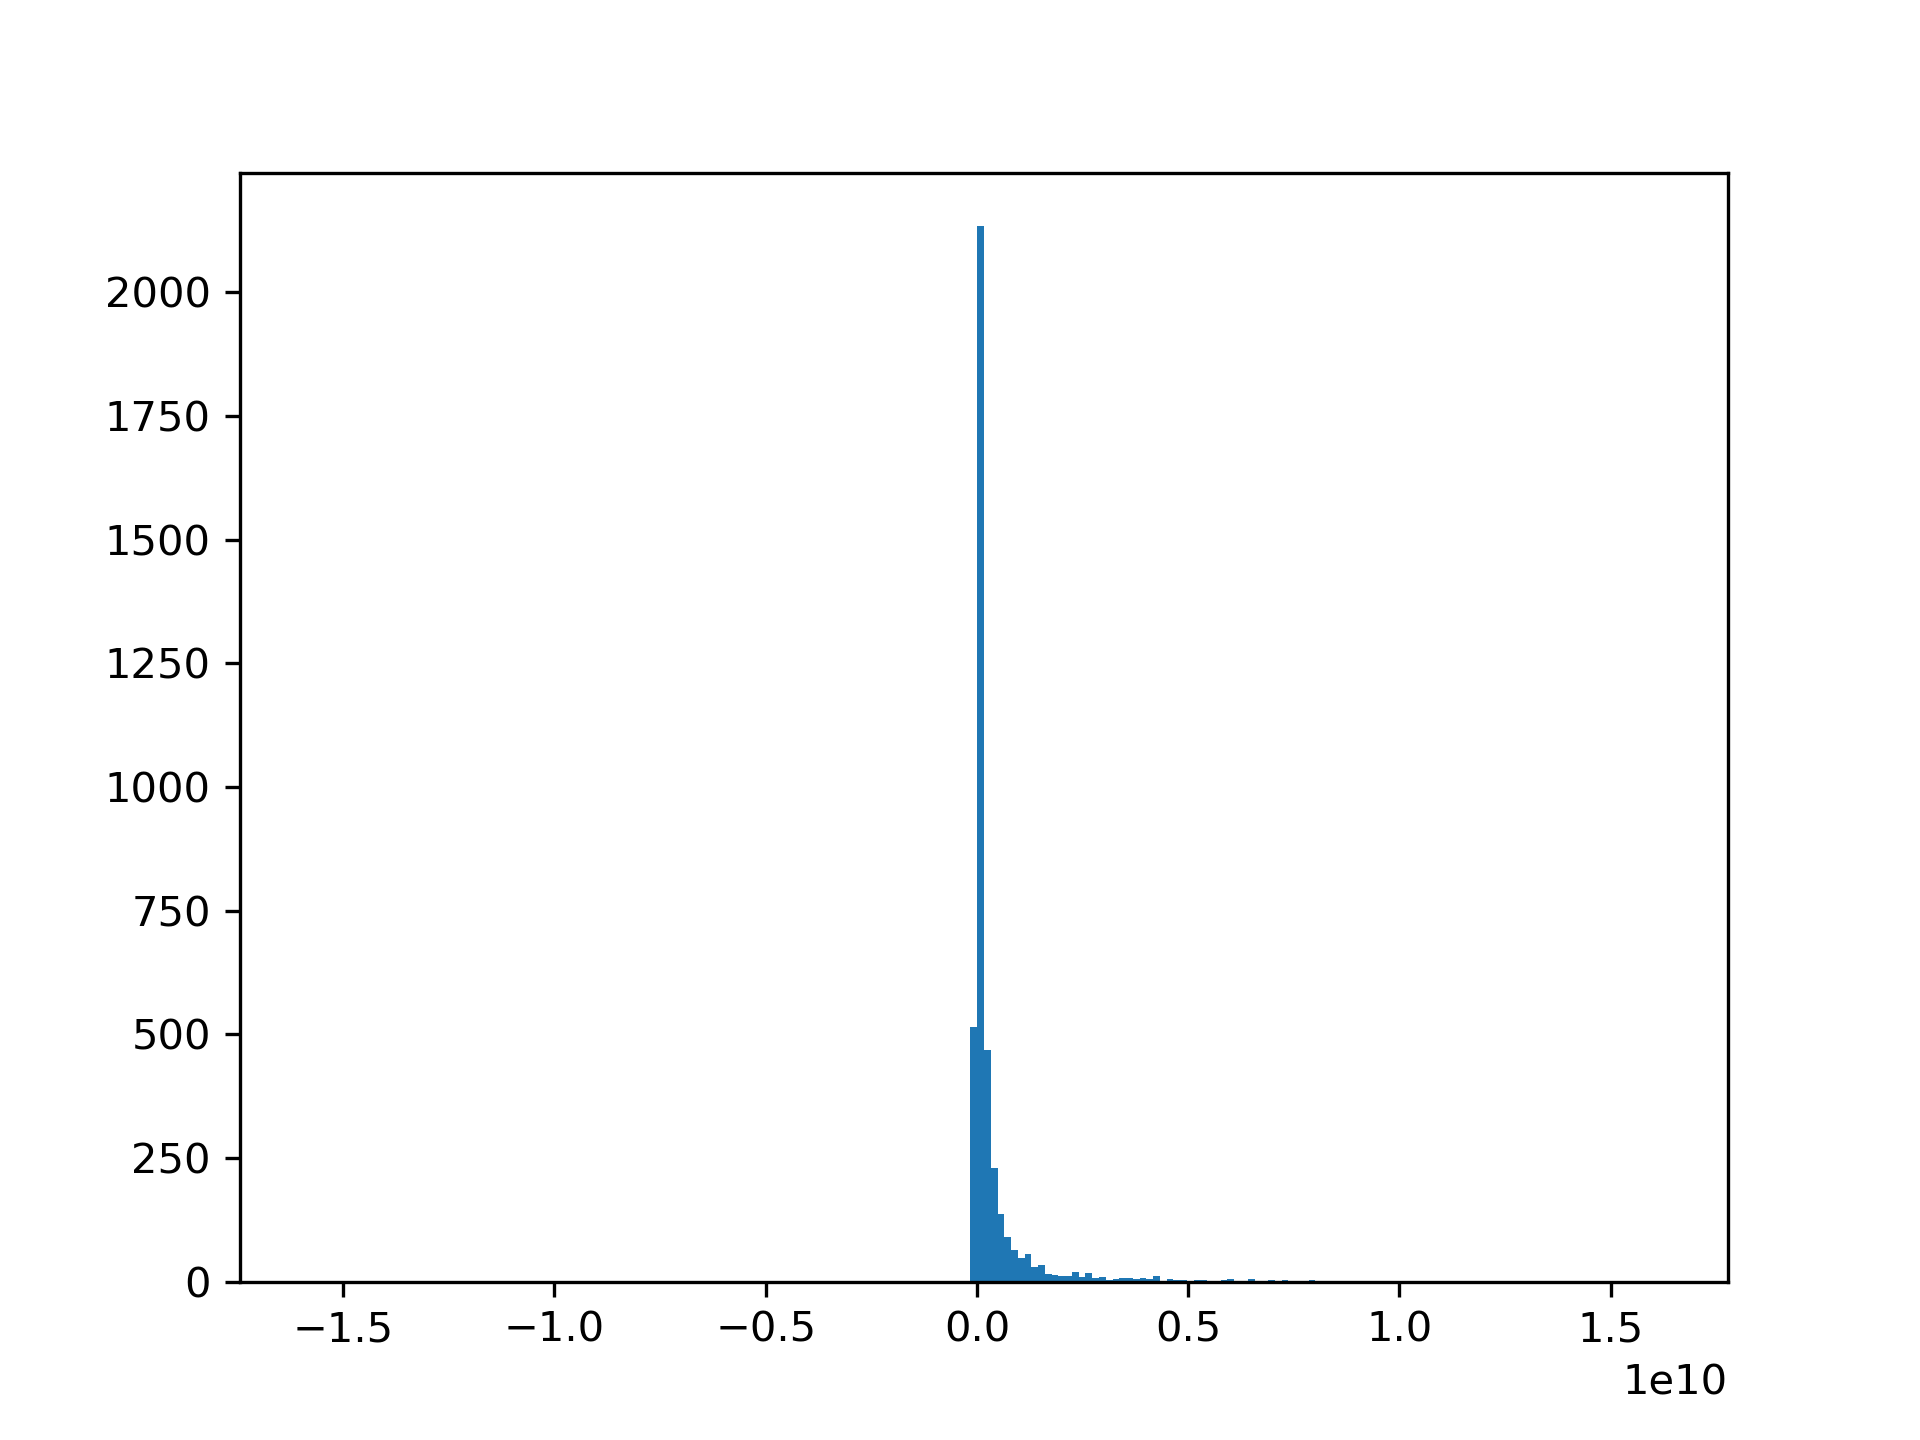
\includegraphics[width=\linewidth]{variables/Cash and cash equivalents.png}
    \caption{Histogram Cash and cash equivalents }
\end{figure}\section{ Short-term investments }

\begin{center}
    \begin{tabular}{|c | c|} 
    \hline
    Statystyka & Wartość \\
    \hline\hline
    Średnia arytmetyczna & 1265001389.1175883 \\ 
    \hline
    Odchylenie standardowe & 14620262143.11258 \\
    \hline
    Kwartyl dolny & 0.0 \\
    \hline
    Mediana & 0.0 \\
    \hline
    Kwartyl górny & 18792375.0 \\
    \hline
    Wartość najmniejsza & 0.0 \\
    \hline
    Wartość największa & 407936000000.0 \\
    \hline
   \end{tabular}
\end{center}

\begin{figure}[h!]
    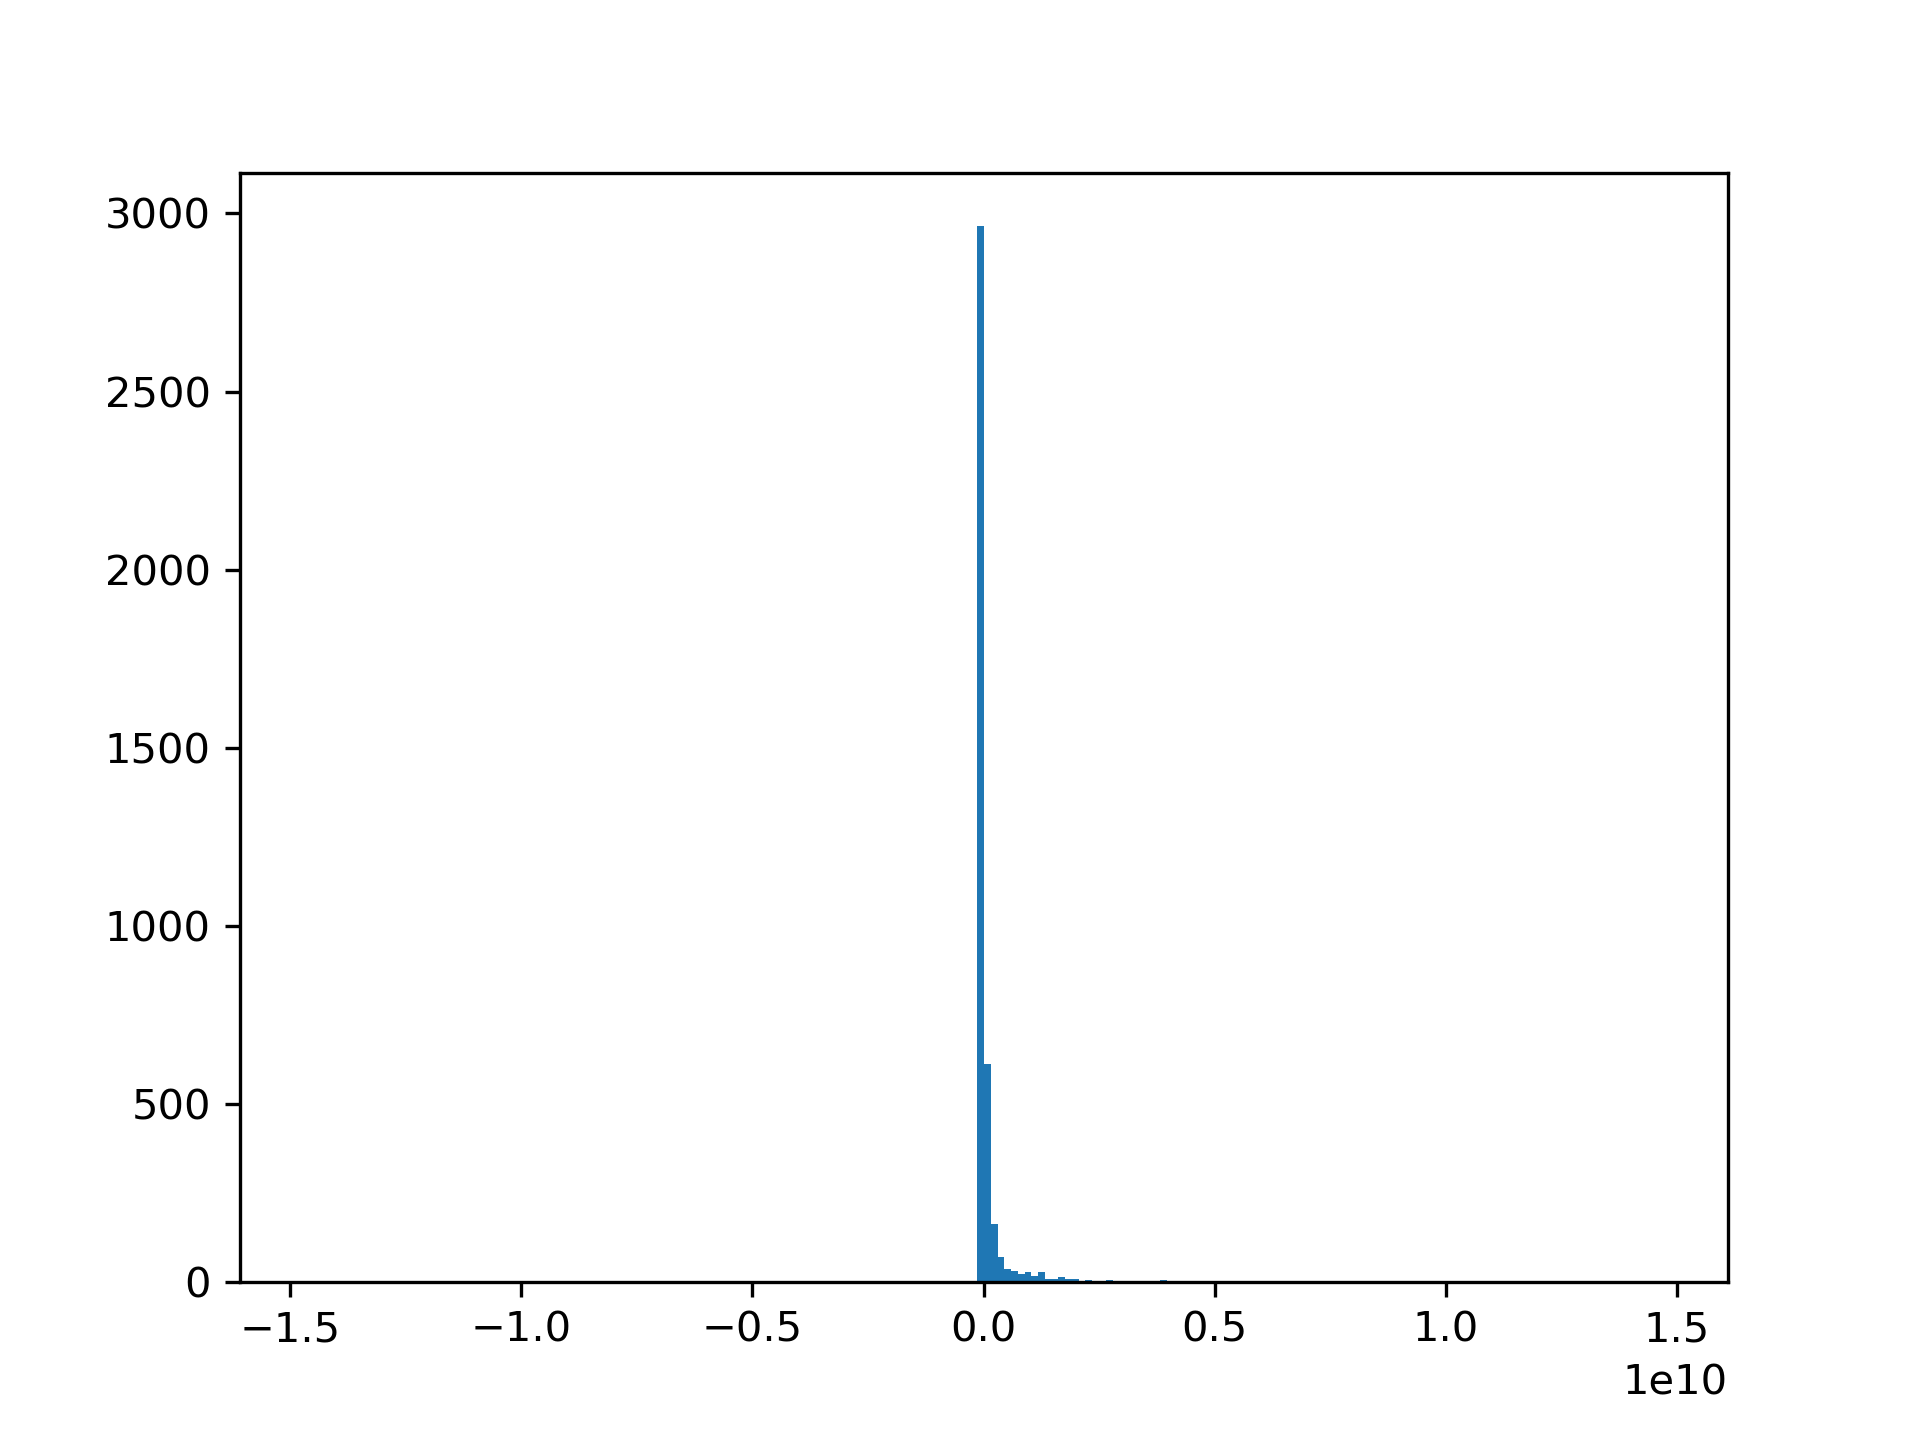
\includegraphics[width=\linewidth]{variables/Short-term investments.png}
    \caption{Histogram Short-term investments }
\end{figure}\section{ Cash and short-term investments }

\begin{center}
    \begin{tabular}{|c | c|} 
    \hline
    Statystyka & Wartość \\
    \hline\hline
    Średnia arytmetyczna & 2829225202.389636 \\ 
    \hline
    Odchylenie standardowe & 27465789685.29632 \\
    \hline
    Kwartyl dolny & 23699750.0 \\
    \hline
    Mediana & 102291000.0 \\
    \hline
    Kwartyl górny & 398814250.0 \\
    \hline
    Wartość najmniejsza & 0.0 \\
    \hline
    Wartość największa & 711732000000.0 \\
    \hline
   \end{tabular}
\end{center}

\begin{figure}[h!]
    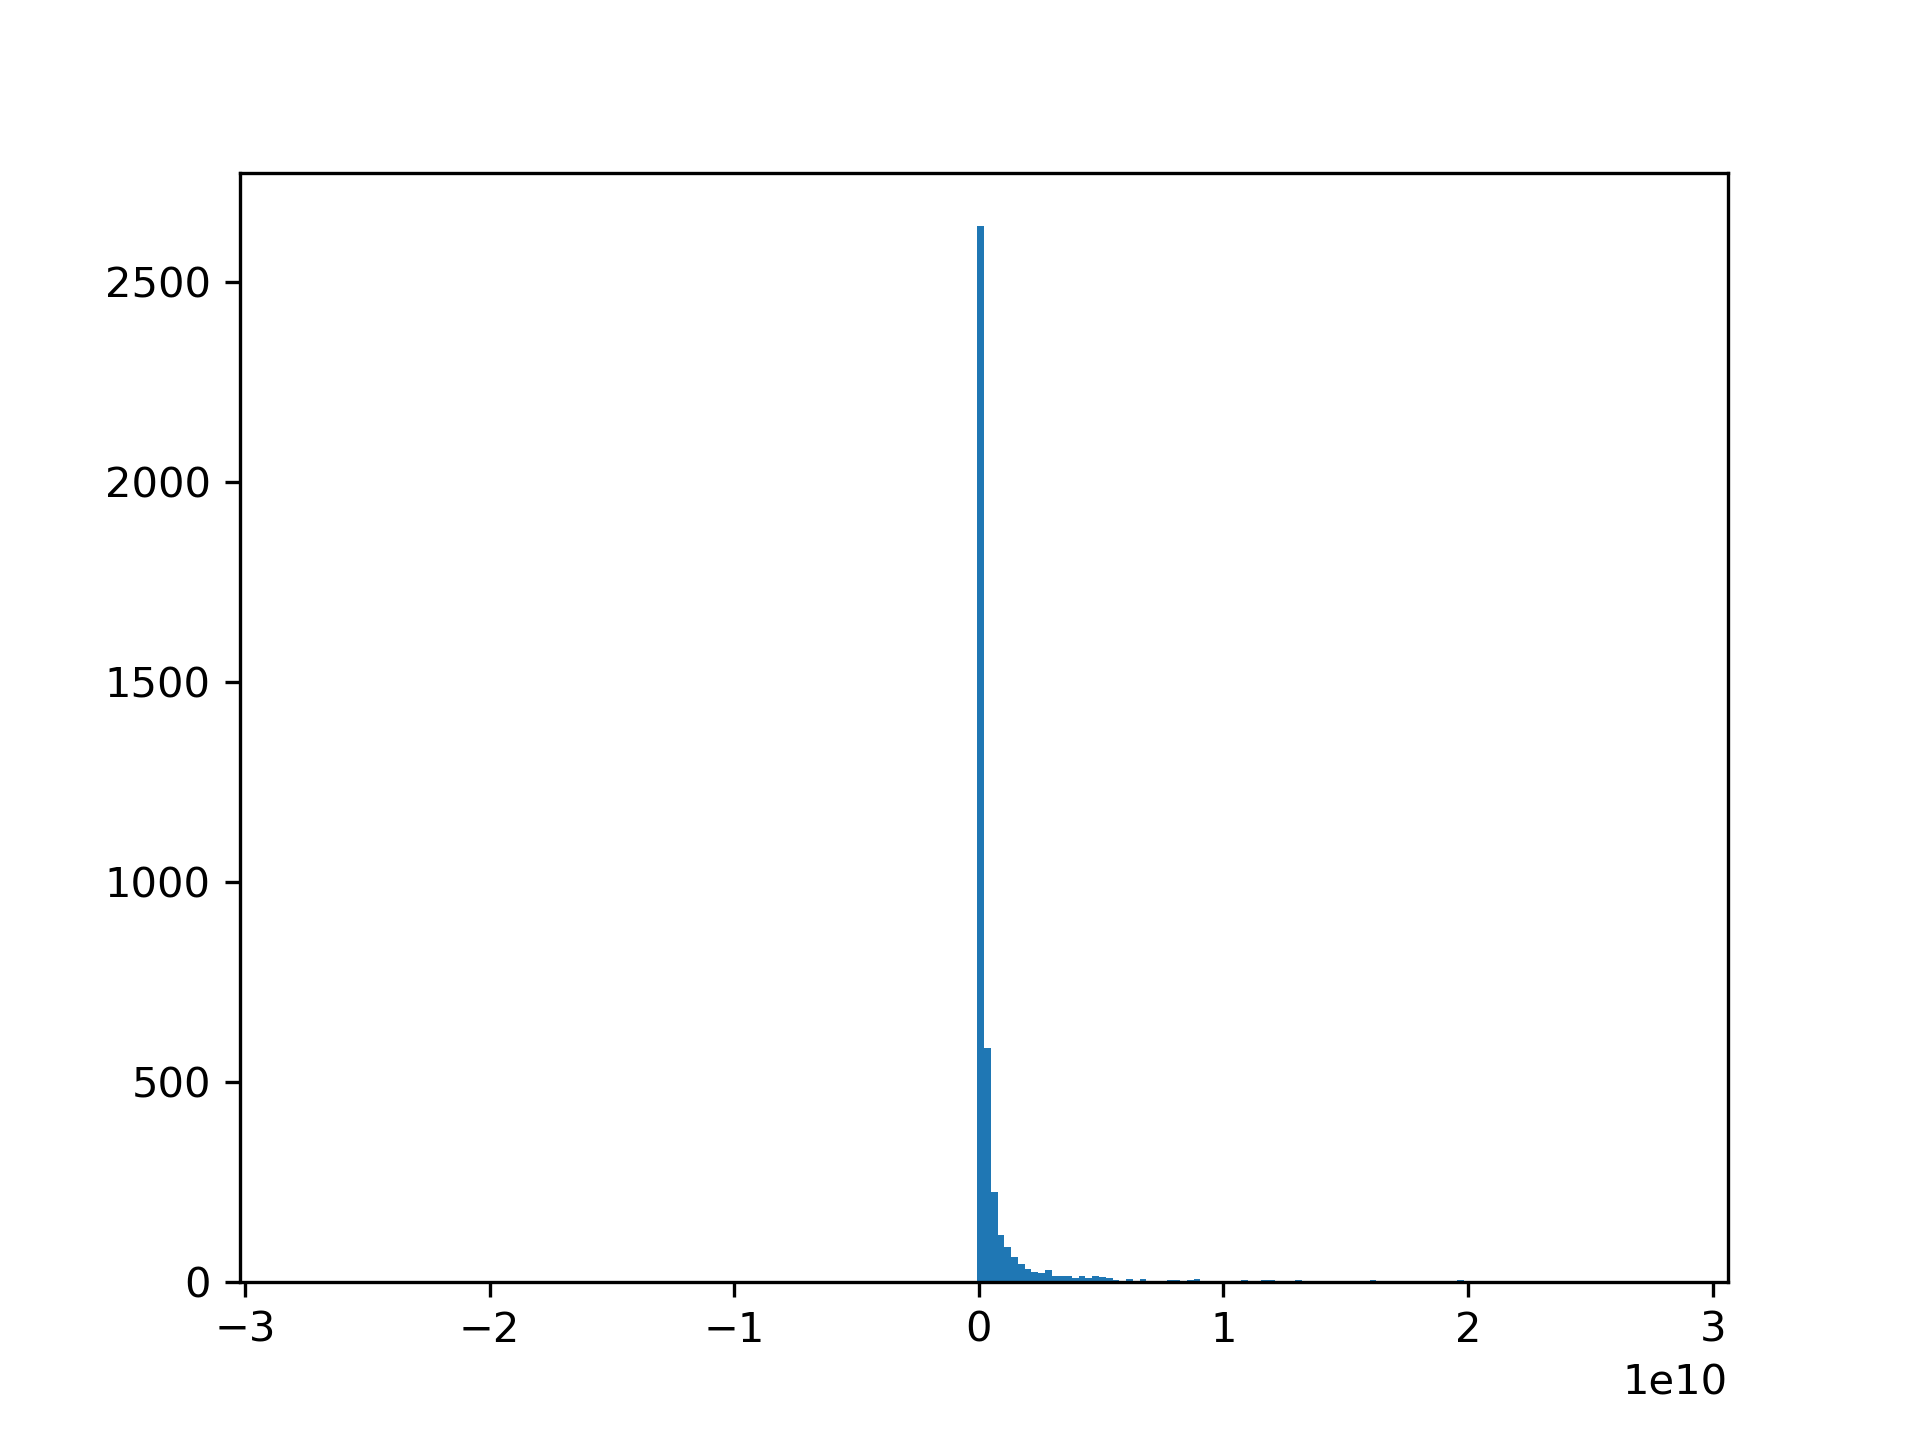
\includegraphics[width=\linewidth]{variables/Cash and short-term investments.png}
    \caption{Histogram Cash and short-term investments }
\end{figure}\section{ Receivables }

\begin{center}
    \begin{tabular}{|c | c|} 
    \hline
    Statystyka & Wartość \\
    \hline\hline
    Średnia arytmetyczna & 932482913.4200954 \\ 
    \hline
    Odchylenie standardowe & 5469197894.978164 \\
    \hline
    Kwartyl dolny & 2411510.339075 \\
    \hline
    Mediana & 52871500.0 \\
    \hline
    Kwartyl górny & 312146500.0 \\
    \hline
    Wartość najmniejsza & 0.0 \\
    \hline
    Wartość największa & 162357737657.8846 \\
    \hline
   \end{tabular}
\end{center}

\begin{figure}[h!]
    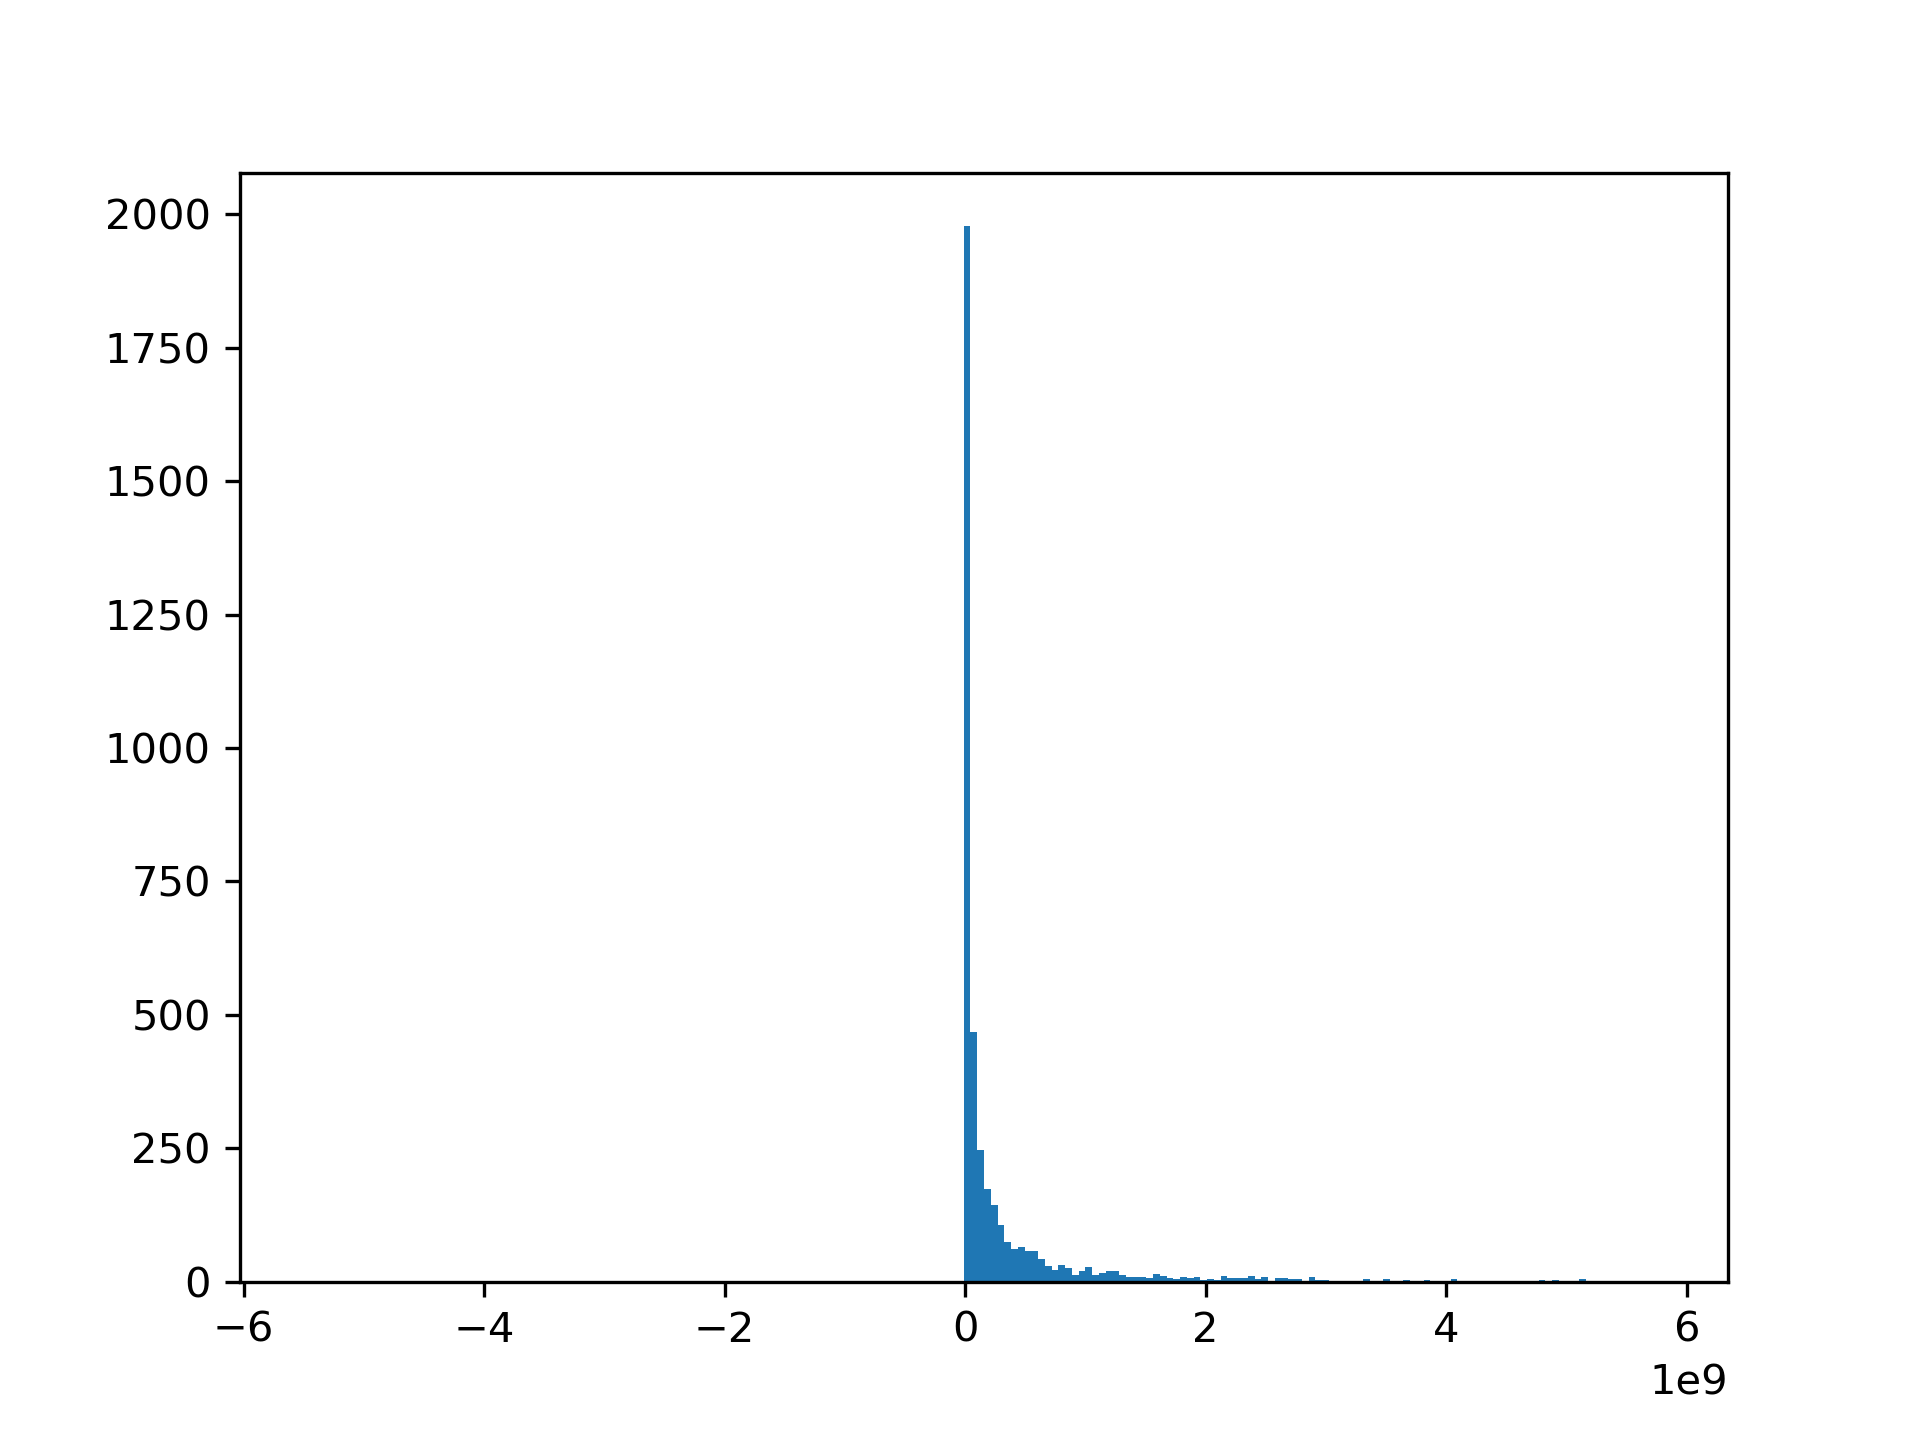
\includegraphics[width=\linewidth]{variables/Receivables.png}
    \caption{Histogram Receivables }
\end{figure}\section{ Inventories }

\begin{center}
    \begin{tabular}{|c | c|} 
    \hline
    Statystyka & Wartość \\
    \hline\hline
    Średnia arytmetyczna & 611087241.5195872 \\ 
    \hline
    Odchylenie standardowe & 14326339209.822145 \\
    \hline
    Kwartyl dolny & 0.0 \\
    \hline
    Mediana & 1599500.0 \\
    \hline
    Kwartyl górny & 110475000.0 \\
    \hline
    Wartość najmniejsza & 0.0 \\
    \hline
    Wartość największa & 912000000000.0 \\
    \hline
   \end{tabular}
\end{center}

\begin{figure}[h!]
    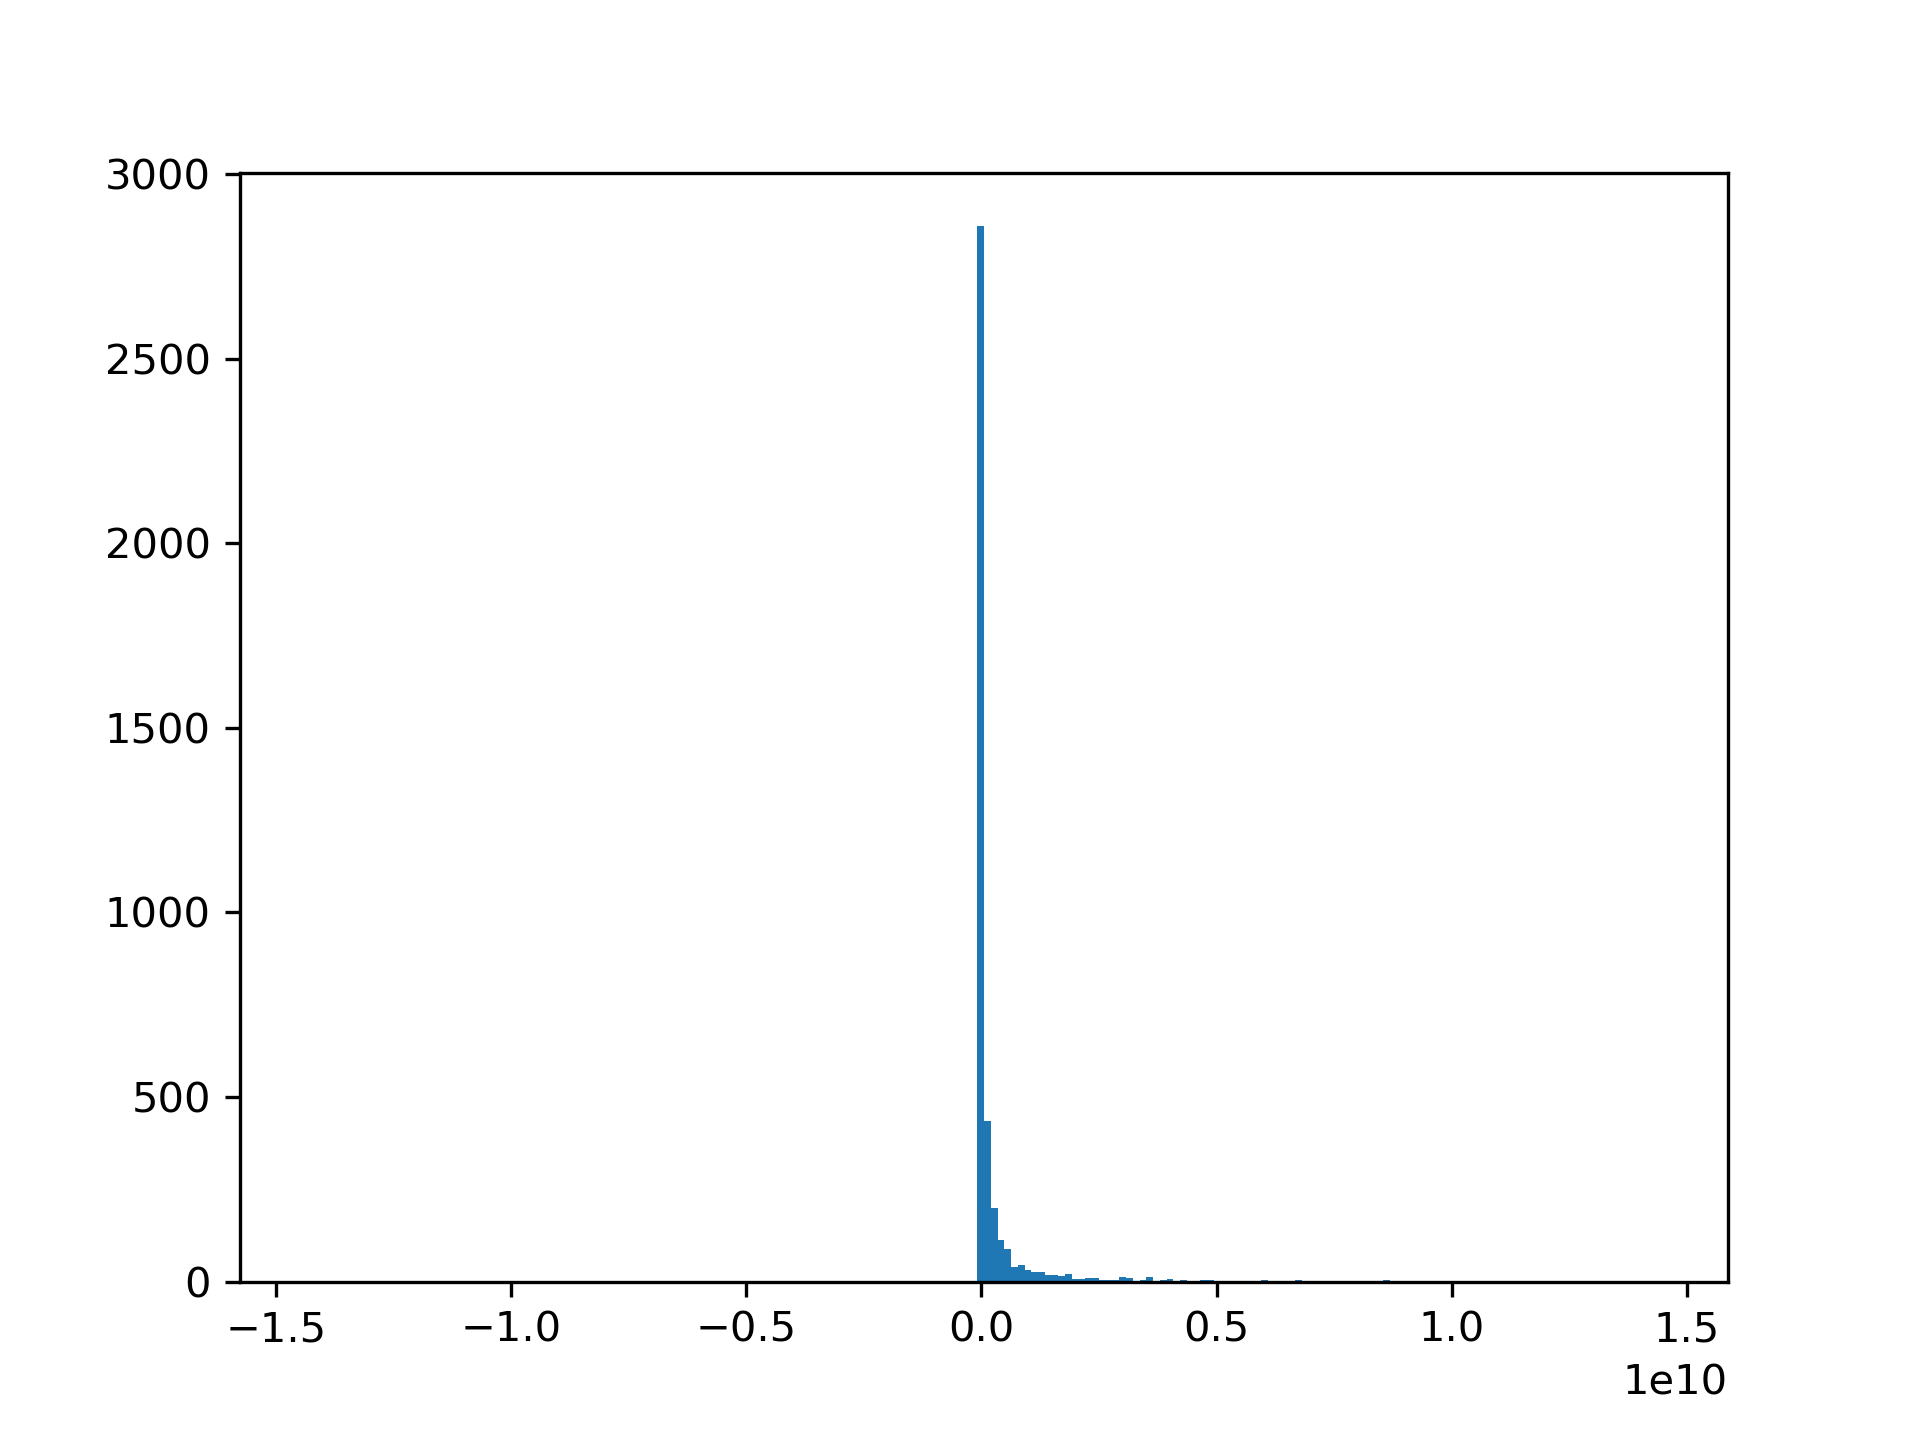
\includegraphics[width=\linewidth]{variables/Inventories.png}
    \caption{Histogram Inventories }
\end{figure}\section{ Total current assets }

\begin{center}
    \begin{tabular}{|c | c|} 
    \hline
    Statystyka & Wartość \\
    \hline\hline
    Średnia arytmetyczna & 5786357909.973802 \\ 
    \hline
    Odchylenie standardowe & 48212335572.54542 \\
    \hline
    Kwartyl dolny & 76512250.0 \\
    \hline
    Mediana & 309827000.0 \\
    \hline
    Kwartyl górny & 1327895000.0 \\
    \hline
    Wartość najmniejsza & 0.0 \\
    \hline
    Wartość największa & 1181015000000.0 \\
    \hline
   \end{tabular}
\end{center}

\begin{figure}[h!]
    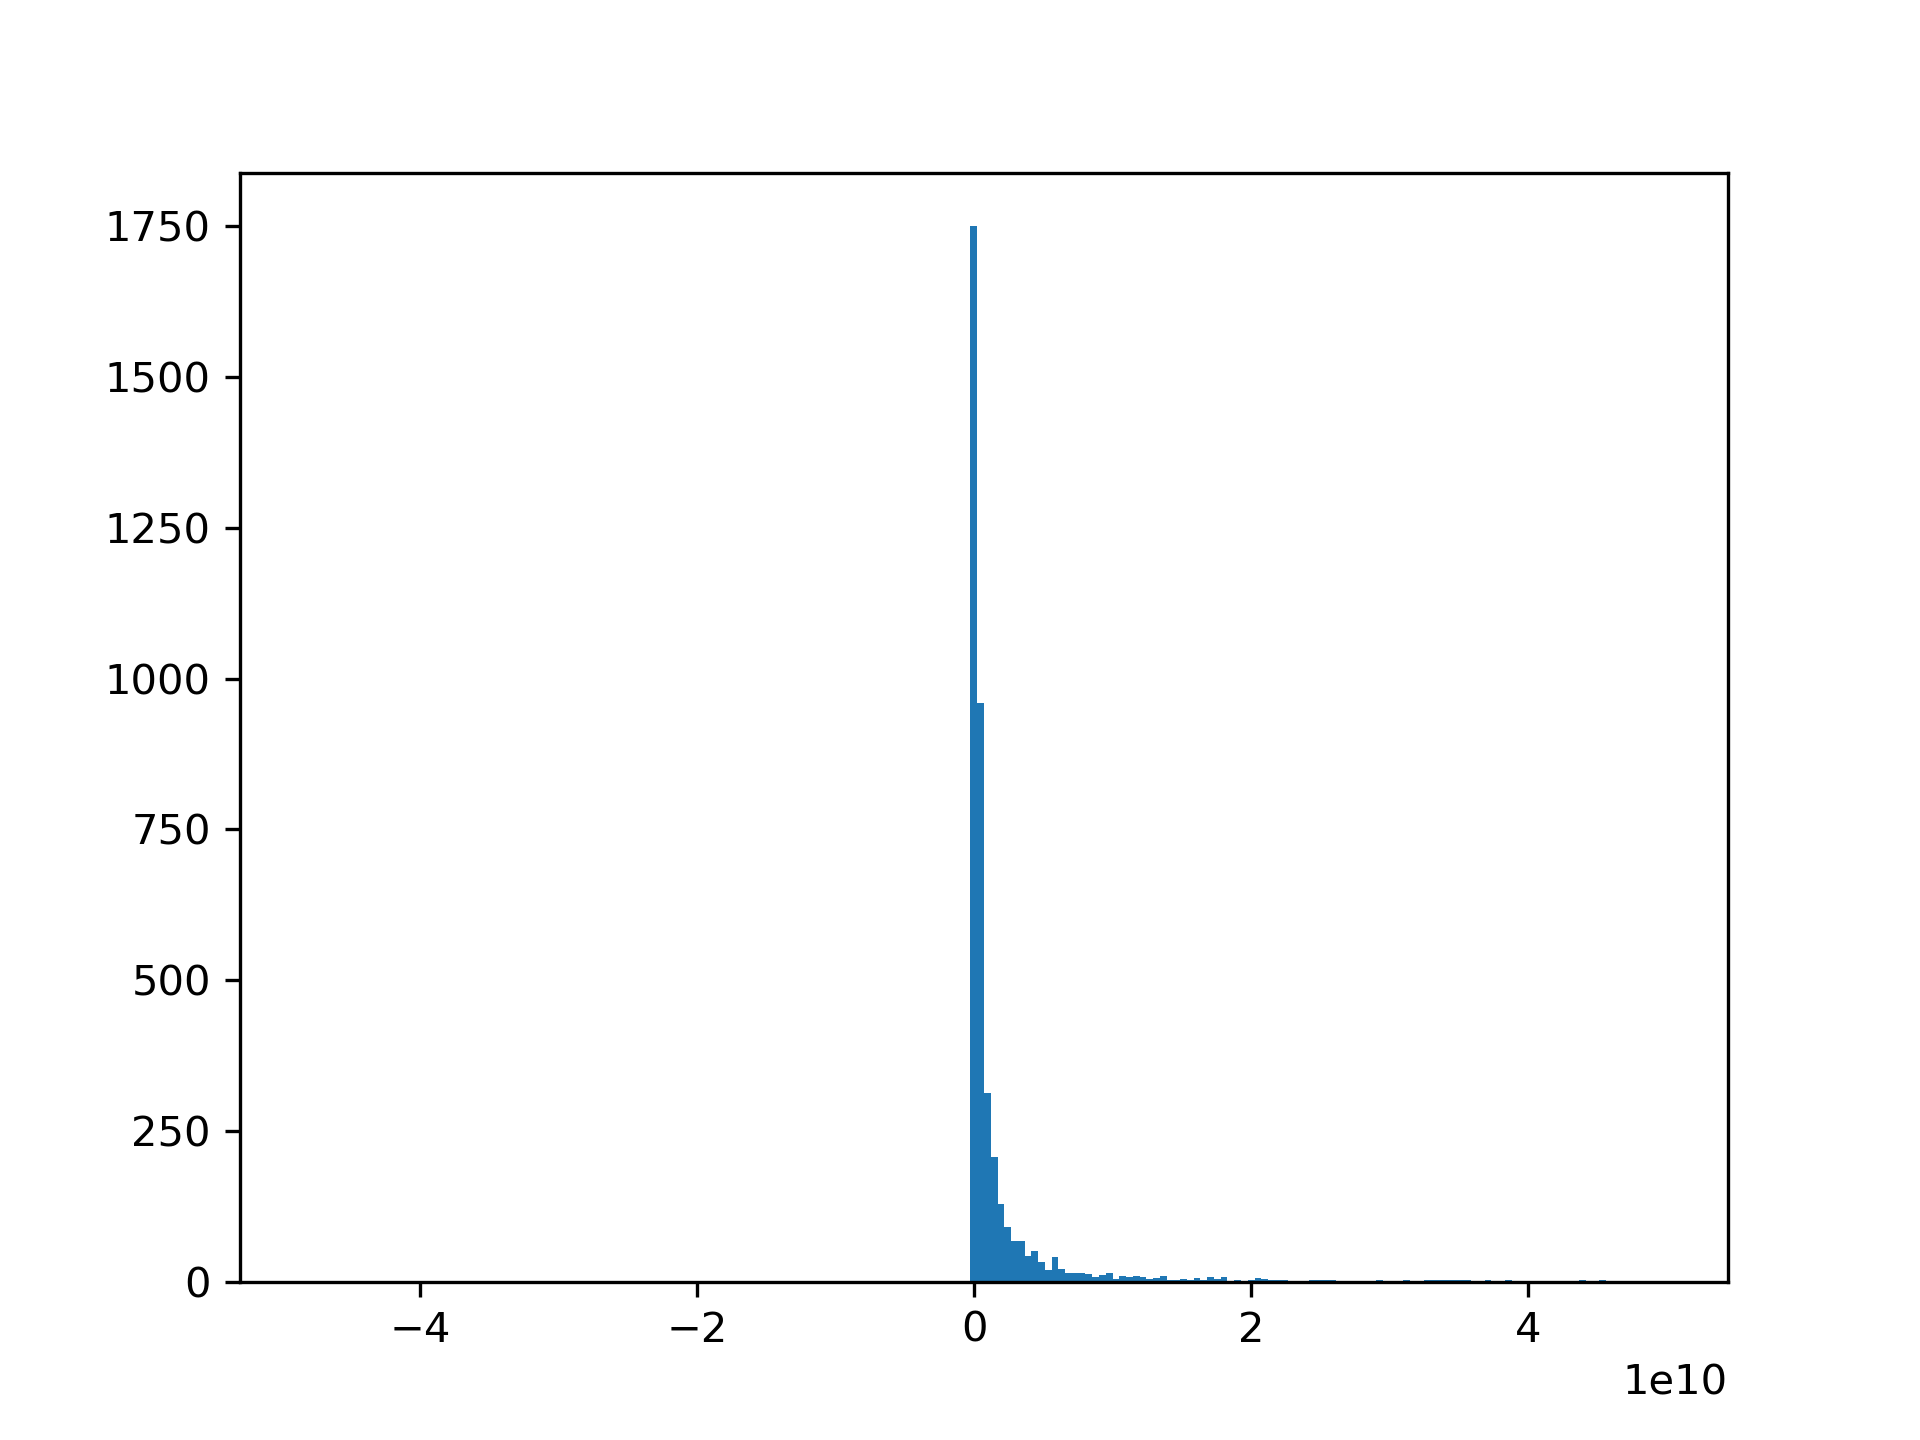
\includegraphics[width=\linewidth]{variables/Total current assets.png}
    \caption{Histogram Total current assets }
\end{figure}\section{ Property, Plant and Equipment Net }

\begin{center}
    \begin{tabular}{|c | c|} 
    \hline
    Statystyka & Wartość \\
    \hline\hline
    Średnia arytmetyczna & 2537459772.849702 \\ 
    \hline
    Odchylenie standardowe & 11080280127.469368 \\
    \hline
    Kwartyl dolny & 10268000.0 \\
    \hline
    Mediana & 106325183.90805 \\
    \hline
    Kwartyl górny & 920573673.4693999 \\
    \hline
    Wartość najmniejsza & 0.0 \\
    \hline
    Wartość największa & 247101000000.0 \\
    \hline
   \end{tabular}
\end{center}

\begin{figure}[h!]
    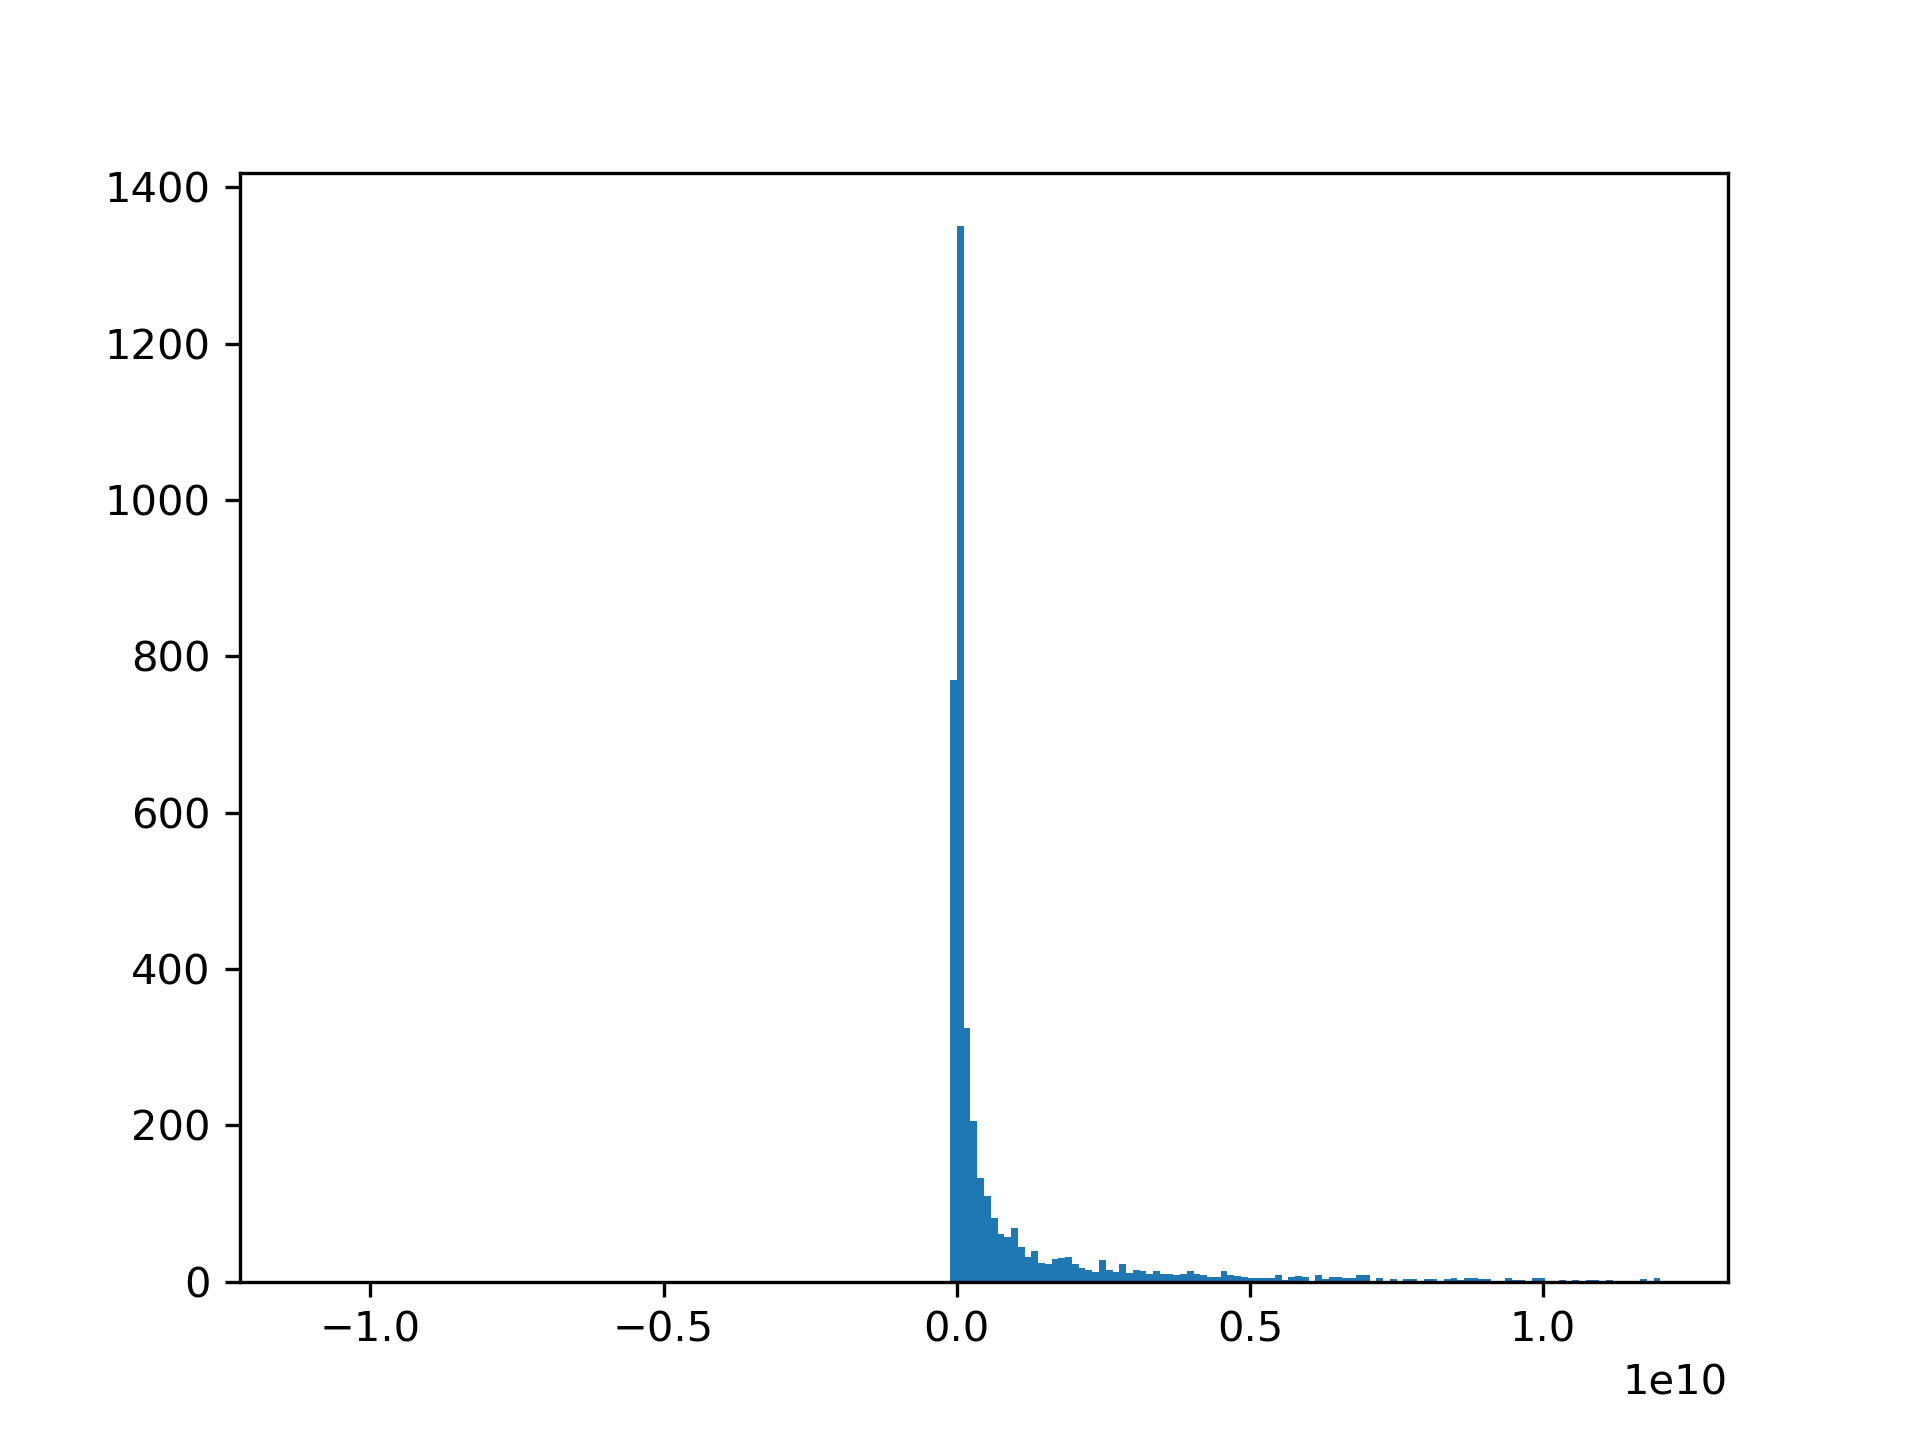
\includegraphics[width=\linewidth]{variables/Property, Plant _ Equipment Net.png}
    \caption{Histogram Property, Plant and Equipment Net }
\end{figure}\section{ Goodwill and Intangible Assets }

\begin{center}
    \begin{tabular}{|c | c|} 
    \hline
    Statystyka & Wartość \\
    \hline\hline
    Średnia arytmetyczna & 1887266959.038447 \\ 
    \hline
    Odchylenie standardowe & 9307929837.522596 \\
    \hline
    Kwartyl dolny & 0.0 \\
    \hline
    Mediana & 49119500.0 \\
    \hline
    Kwartyl górny & 596607090.9091251 \\
    \hline
    Wartość najmniejsza & 0.0 \\
    \hline
    Wartość największa & 293128000000.0 \\
    \hline
   \end{tabular}
\end{center}

\begin{figure}[h!]
    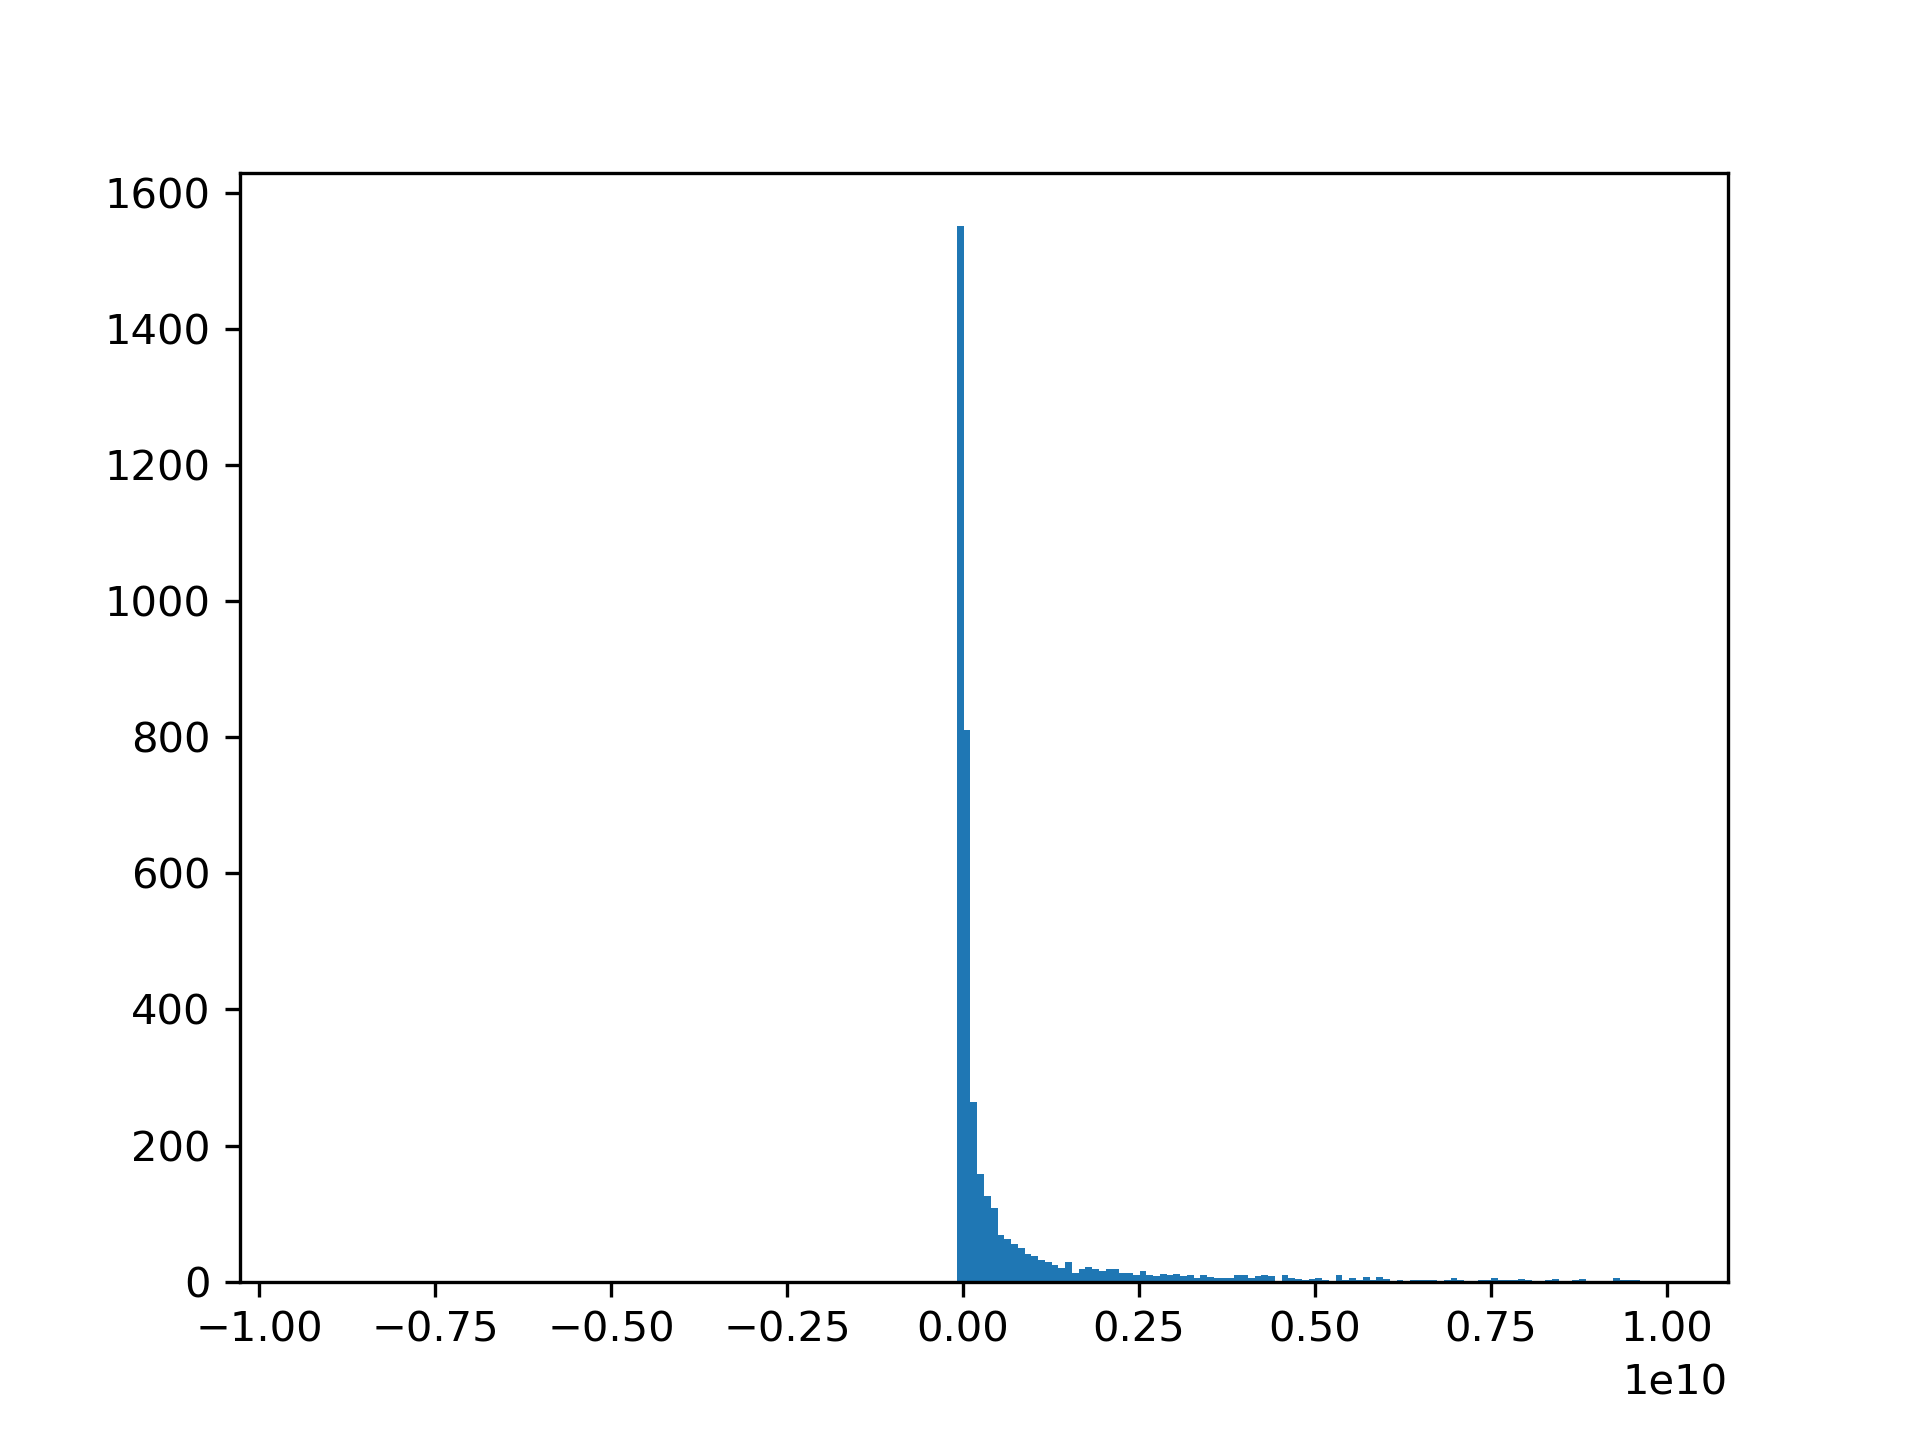
\includegraphics[width=\linewidth]{variables/Goodwill and Intangible Assets.png}
    \caption{Histogram Goodwill and Intangible Assets }
\end{figure}\section{ Long-term investments }

\begin{center}
    \begin{tabular}{|c | c|} 
    \hline
    Statystyka & Wartość \\
    \hline\hline
    Średnia arytmetyczna & 3023774717.503585 \\ 
    \hline
    Odchylenie standardowe & 34666035016.503815 \\
    \hline
    Kwartyl dolny & 0.0 \\
    \hline
    Mediana & 0.0 \\
    \hline
    Kwartyl górny & 64000000.0 \\
    \hline
    Wartość najmniejsza & -80000000.0 \\
    \hline
    Wartość największa & 995000000000.0 \\
    \hline
   \end{tabular}
\end{center}

\begin{figure}[h!]
    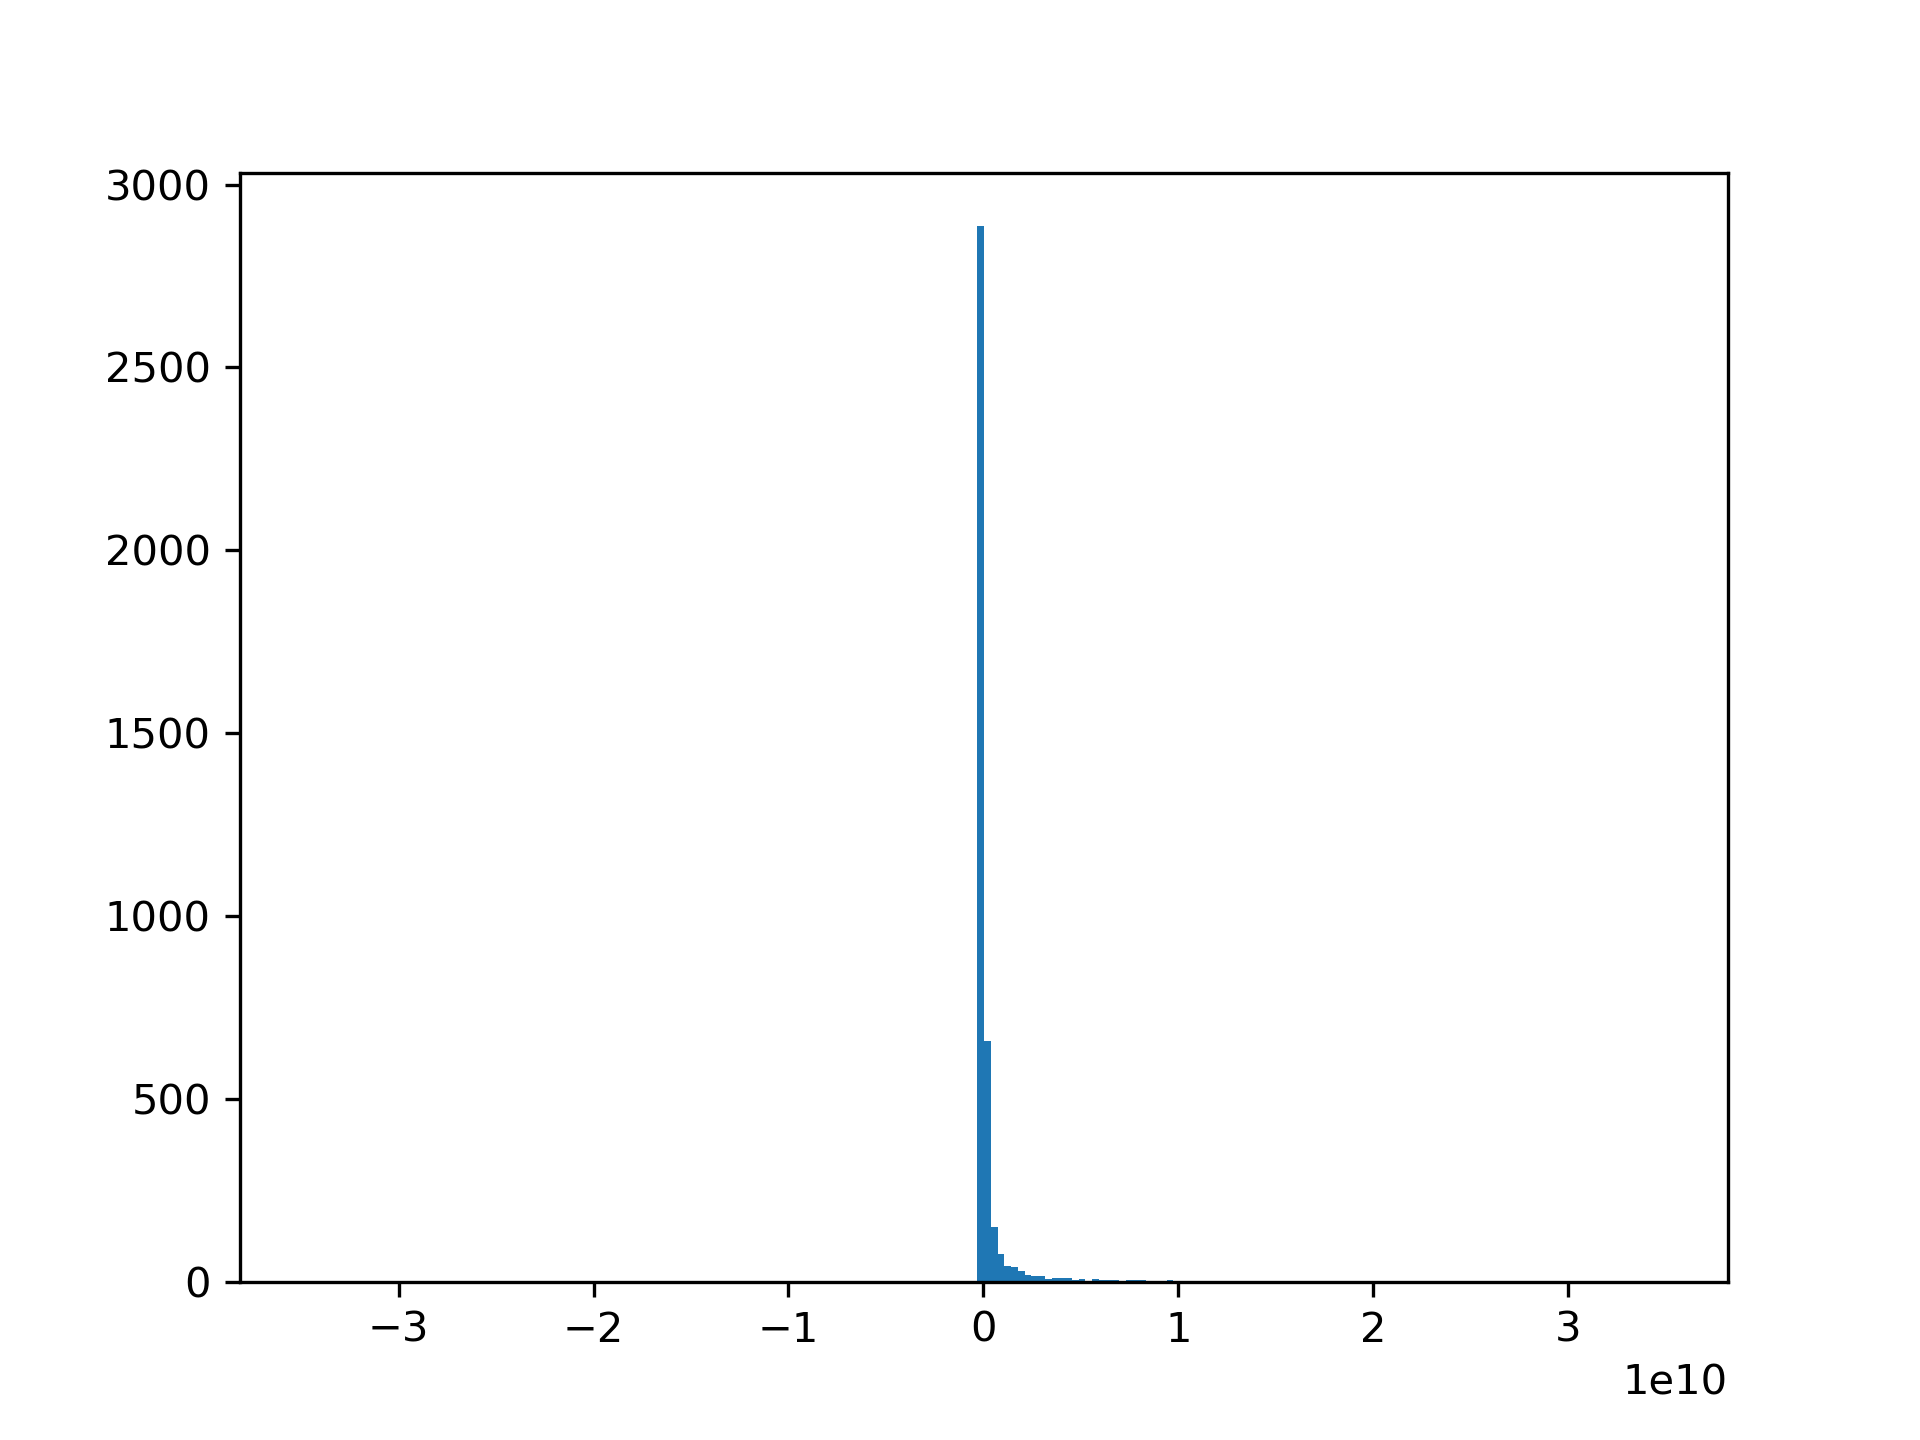
\includegraphics[width=\linewidth]{variables/Long-term investments.png}
    \caption{Histogram Long-term investments }
\end{figure}\section{ Tax assets }

\begin{center}
    \begin{tabular}{|c | c|} 
    \hline
    Statystyka & Wartość \\
    \hline\hline
    Średnia arytmetyczna & 132501425.50655834 \\ 
    \hline
    Odchylenie standardowe & 1038876328.3288385 \\
    \hline
    Kwartyl dolny & 0.0 \\
    \hline
    Mediana & 0.0 \\
    \hline
    Kwartyl górny & 10716750.0 \\
    \hline
    Wartość najmniejsza & 0.0 \\
    \hline
    Wartość największa & 36688981868.8982 \\
    \hline
   \end{tabular}
\end{center}

\begin{figure}[h!]
    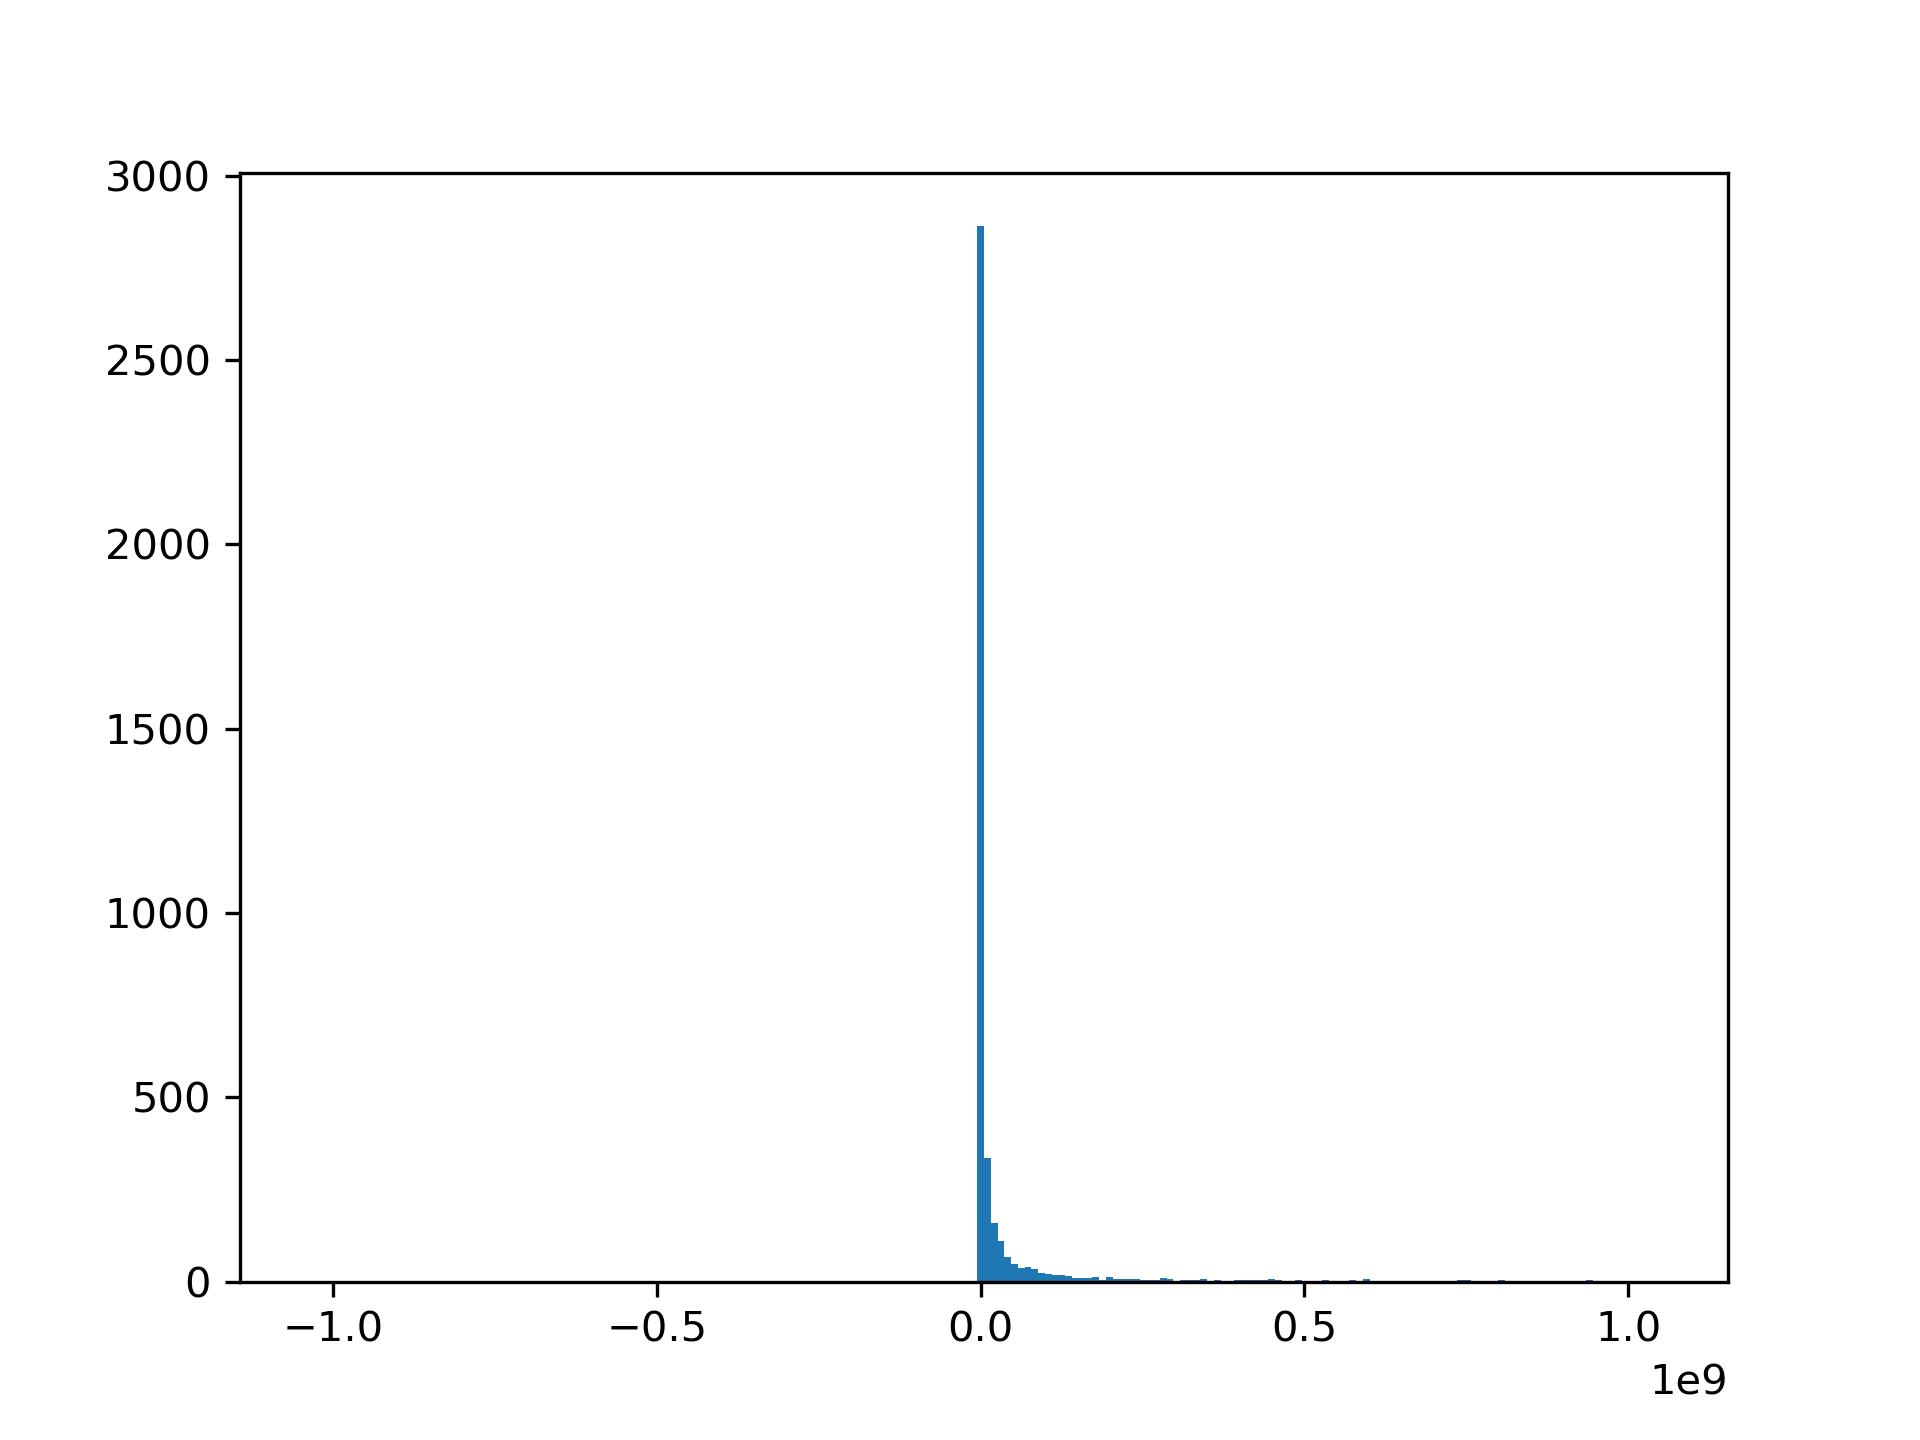
\includegraphics[width=\linewidth]{variables/Tax assets.png}
    \caption{Histogram Tax assets }
\end{figure}\section{ Total assets }

\begin{center}
    \begin{tabular}{|c | c|} 
    \hline
    Statystyka & Wartość \\
    \hline\hline
    Średnia arytmetyczna & 18398621435.798428 \\ 
    \hline
    Odchylenie standardowe & 113789501331.11047 \\
    \hline
    Kwartyl dolny & 253987071.0 \\
    \hline
    Mediana & 1340700500.0 \\
    \hline
    Kwartyl górny & 5676841500.0 \\
    \hline
    Wartość najmniejsza & 299737.0 \\
    \hline
    Wartość największa & 2622532000000.0 \\
    \hline
   \end{tabular}
\end{center}

\begin{figure}[h!]
    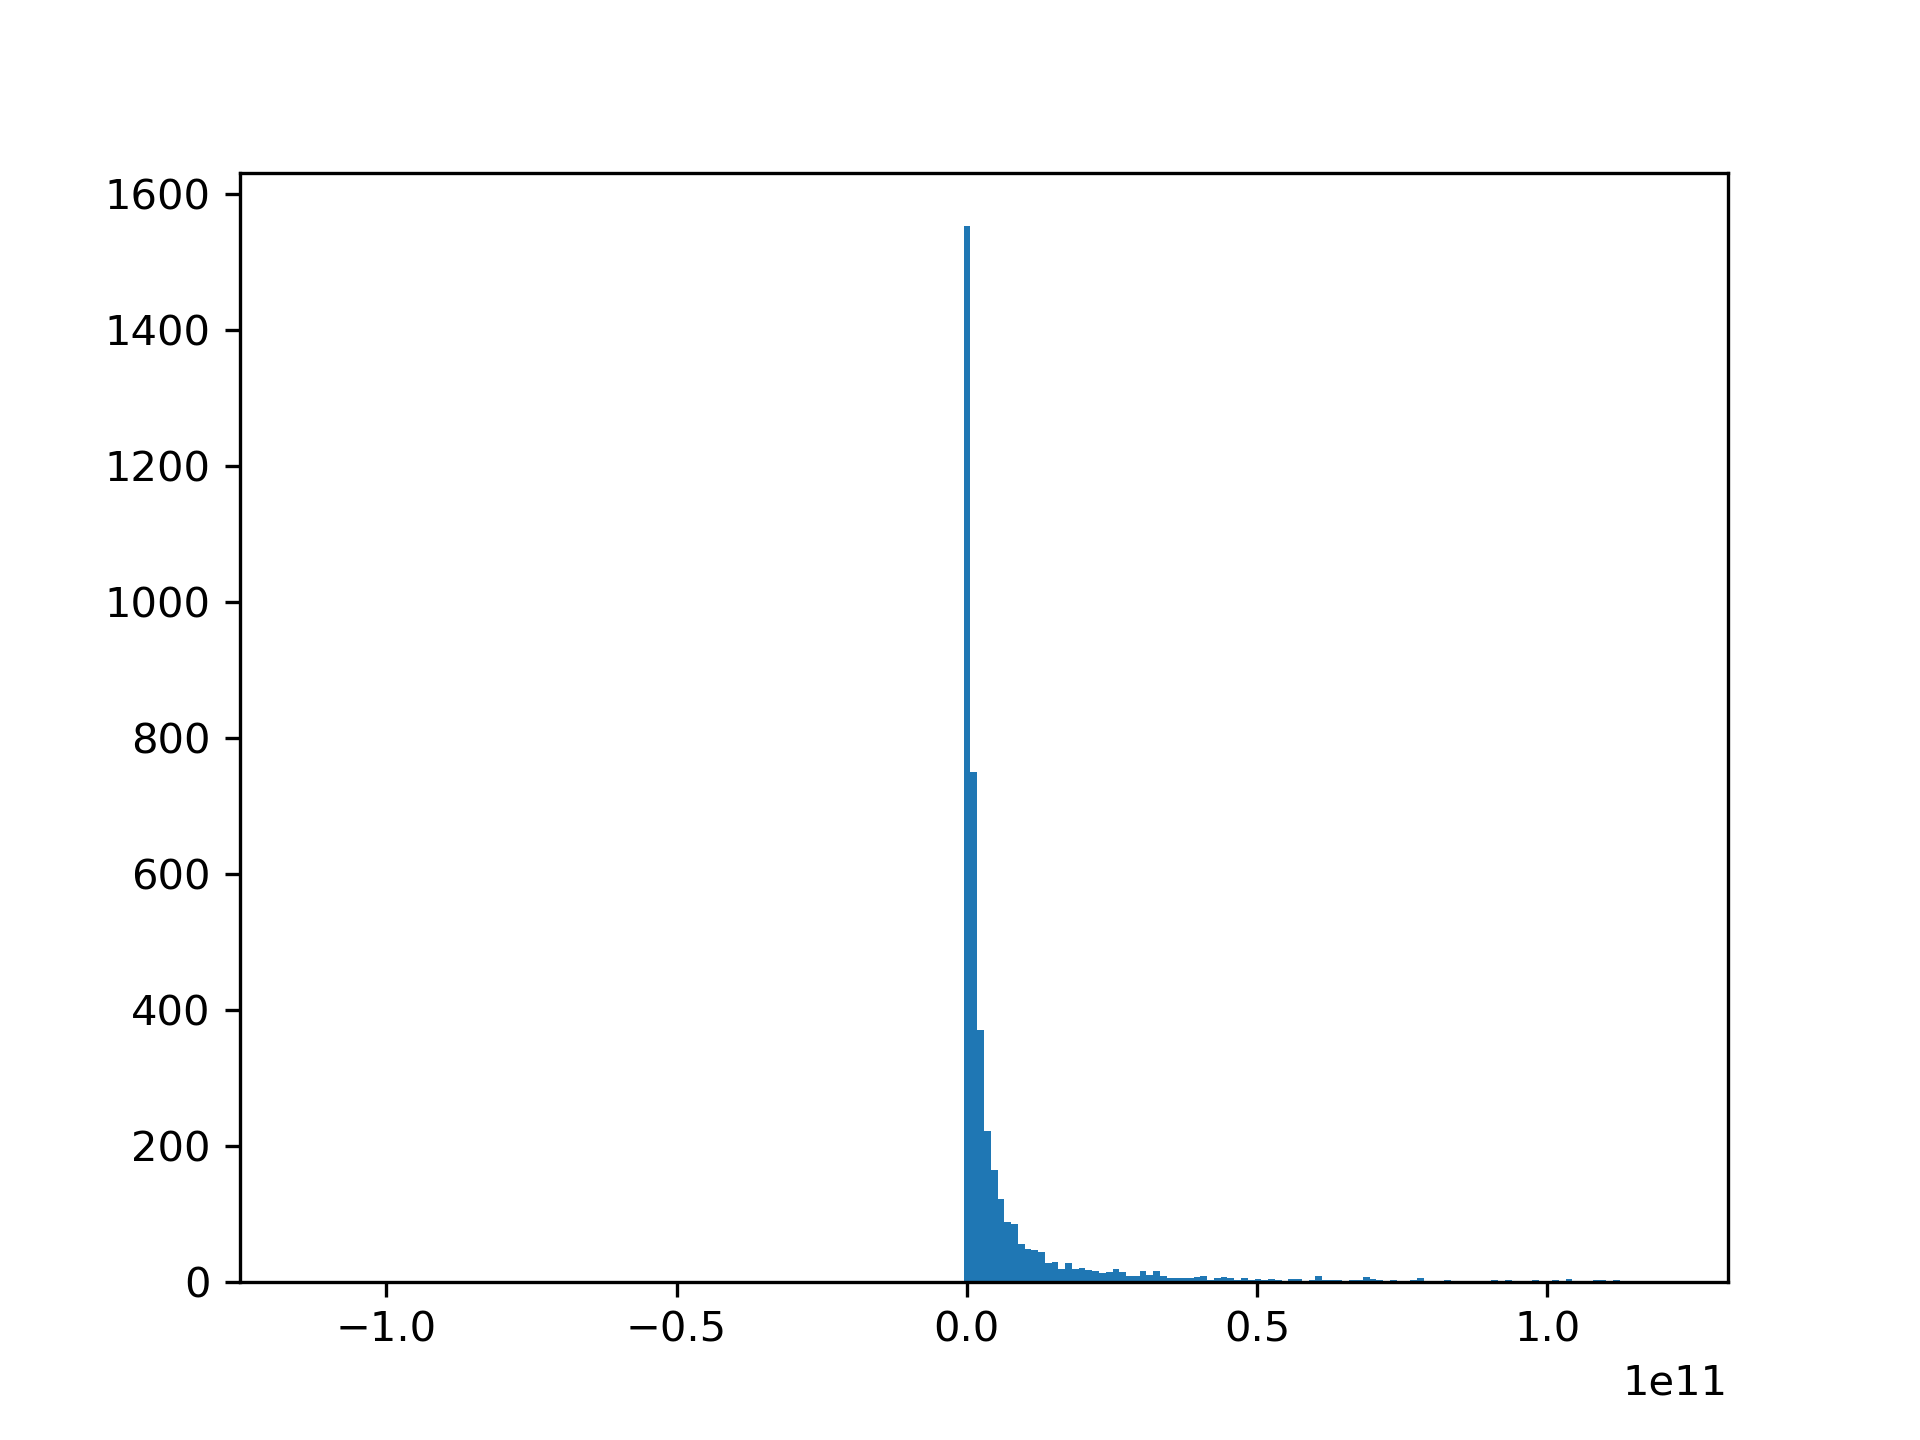
\includegraphics[width=\linewidth]{variables/Total assets.png}
    \caption{Histogram Total assets }
\end{figure}\section{ Payables }

\begin{center}
    \begin{tabular}{|c | c|} 
    \hline
    Statystyka & Wartość \\
    \hline\hline
    Średnia arytmetyczna & 877004164.5090563 \\ 
    \hline
    Odchylenie standardowe & 6207693050.99803 \\
    \hline
    Kwartyl dolny & 3378038.0 \\
    \hline
    Mediana & 30412770.0 \\
    \hline
    Kwartyl górny & 208527000.0 \\
    \hline
    Wartość najmniejsza & -20152030456.8528 \\
    \hline
    Wartość największa & 196710000000.0 \\
    \hline
   \end{tabular}
\end{center}

\begin{figure}[h!]
    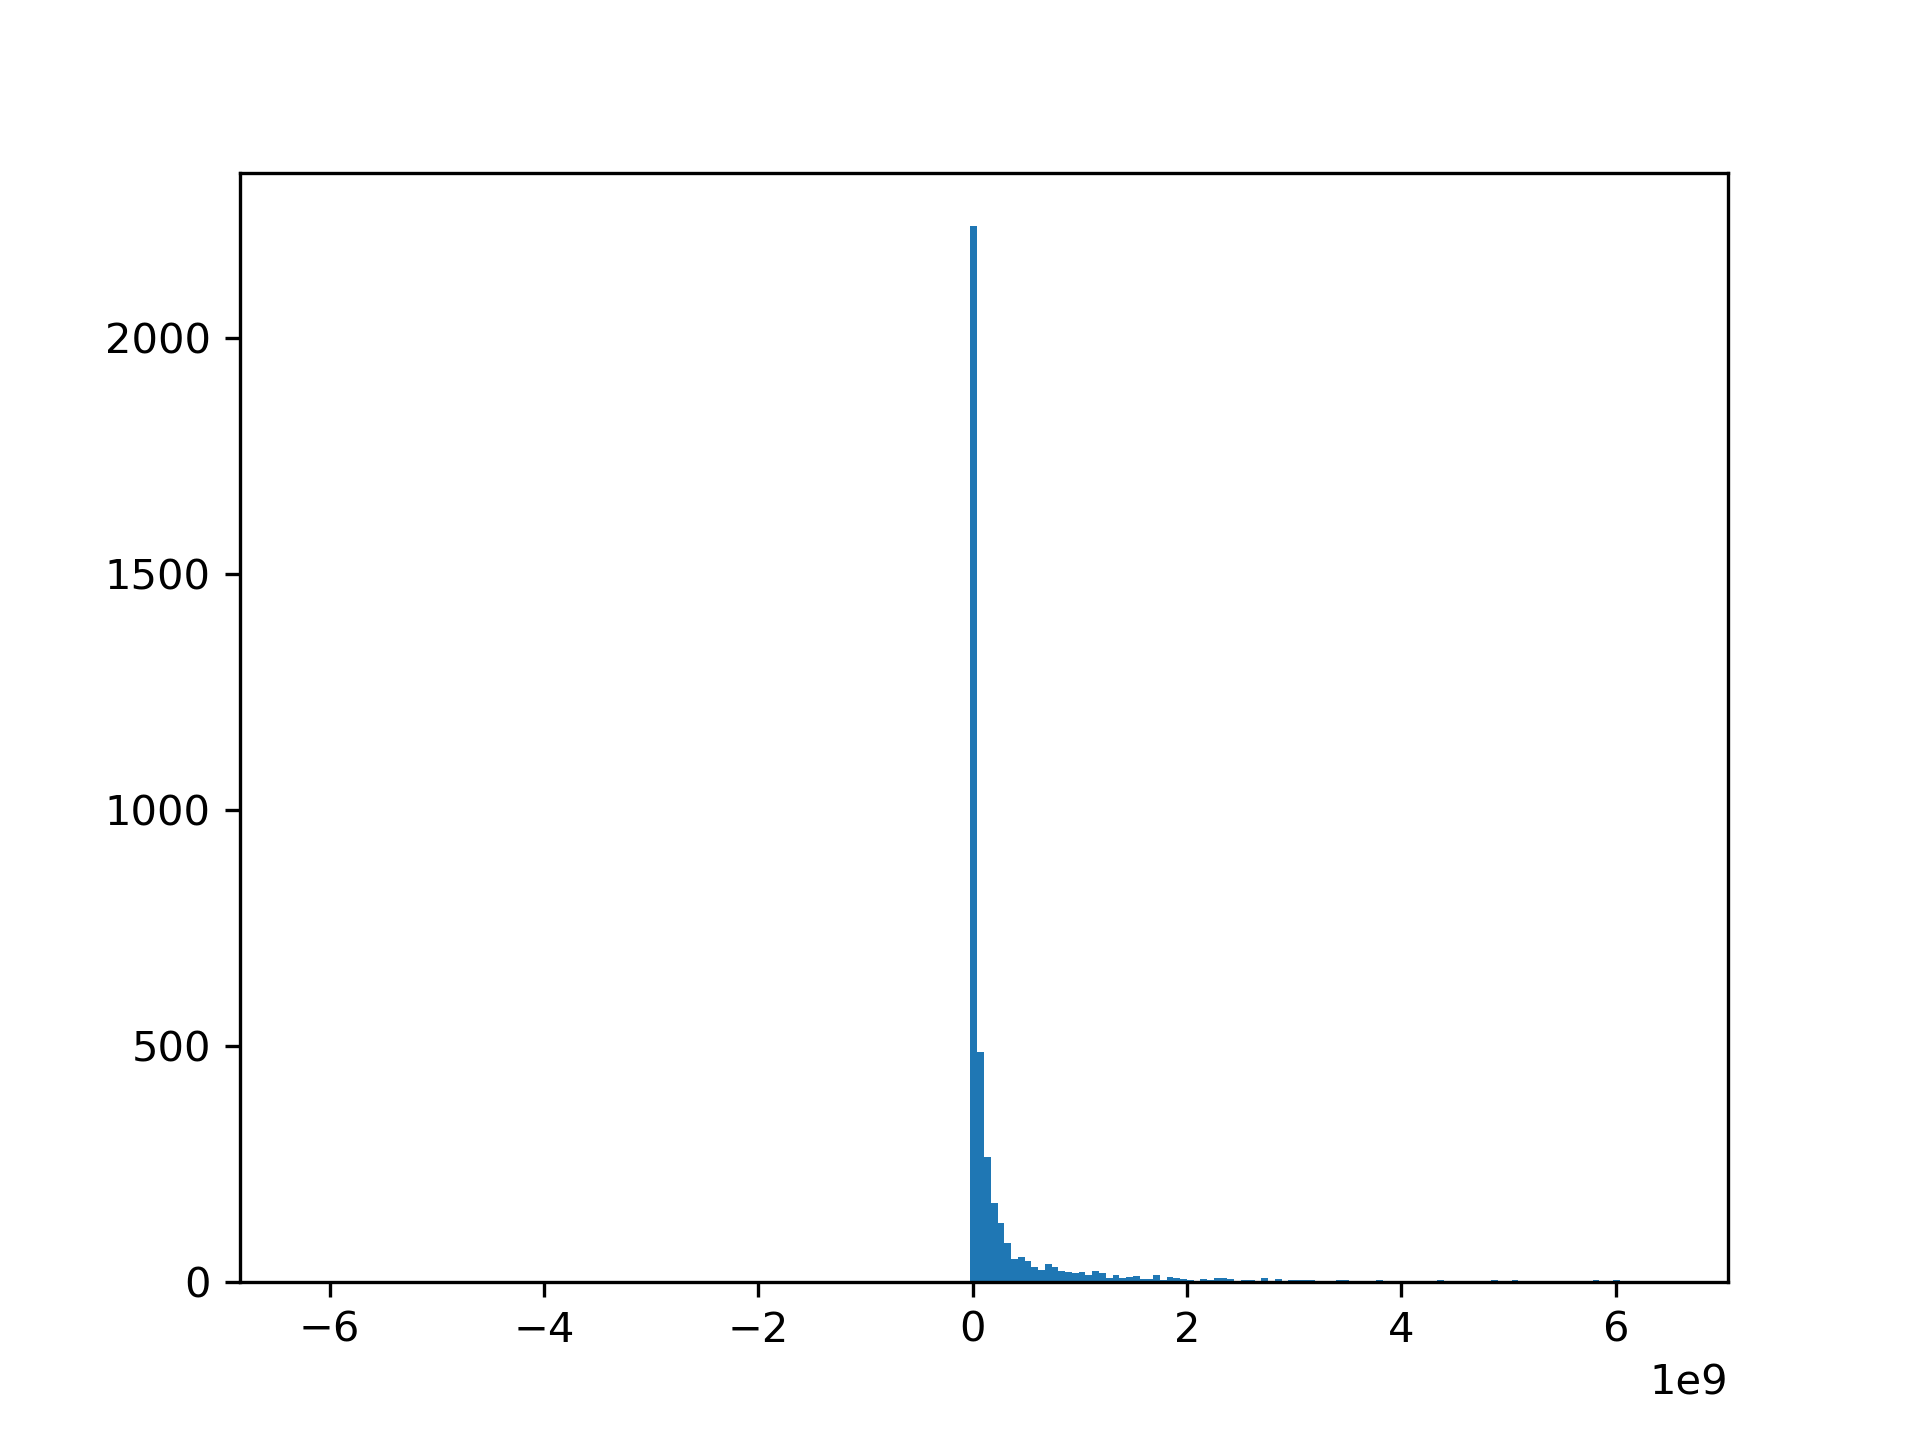
\includegraphics[width=\linewidth]{variables/Payables.png}
    \caption{Histogram Payables }
\end{figure}\section{ Short-term debt }

\begin{center}
    \begin{tabular}{|c | c|} 
    \hline
    Statystyka & Wartość \\
    \hline\hline
    Średnia arytmetyczna & 696774948.3730898 \\ 
    \hline
    Odchylenie standardowe & 6136417671.416339 \\
    \hline
    Kwartyl dolny & 0.0 \\
    \hline
    Mediana & 1853000.0 \\
    \hline
    Kwartyl górny & 46783750.0 \\
    \hline
    Wartość najmniejsza & -1300888324.8731 \\
    \hline
    Wartość największa & 219180000000.0 \\
    \hline
   \end{tabular}
\end{center}

\begin{figure}[h!]
    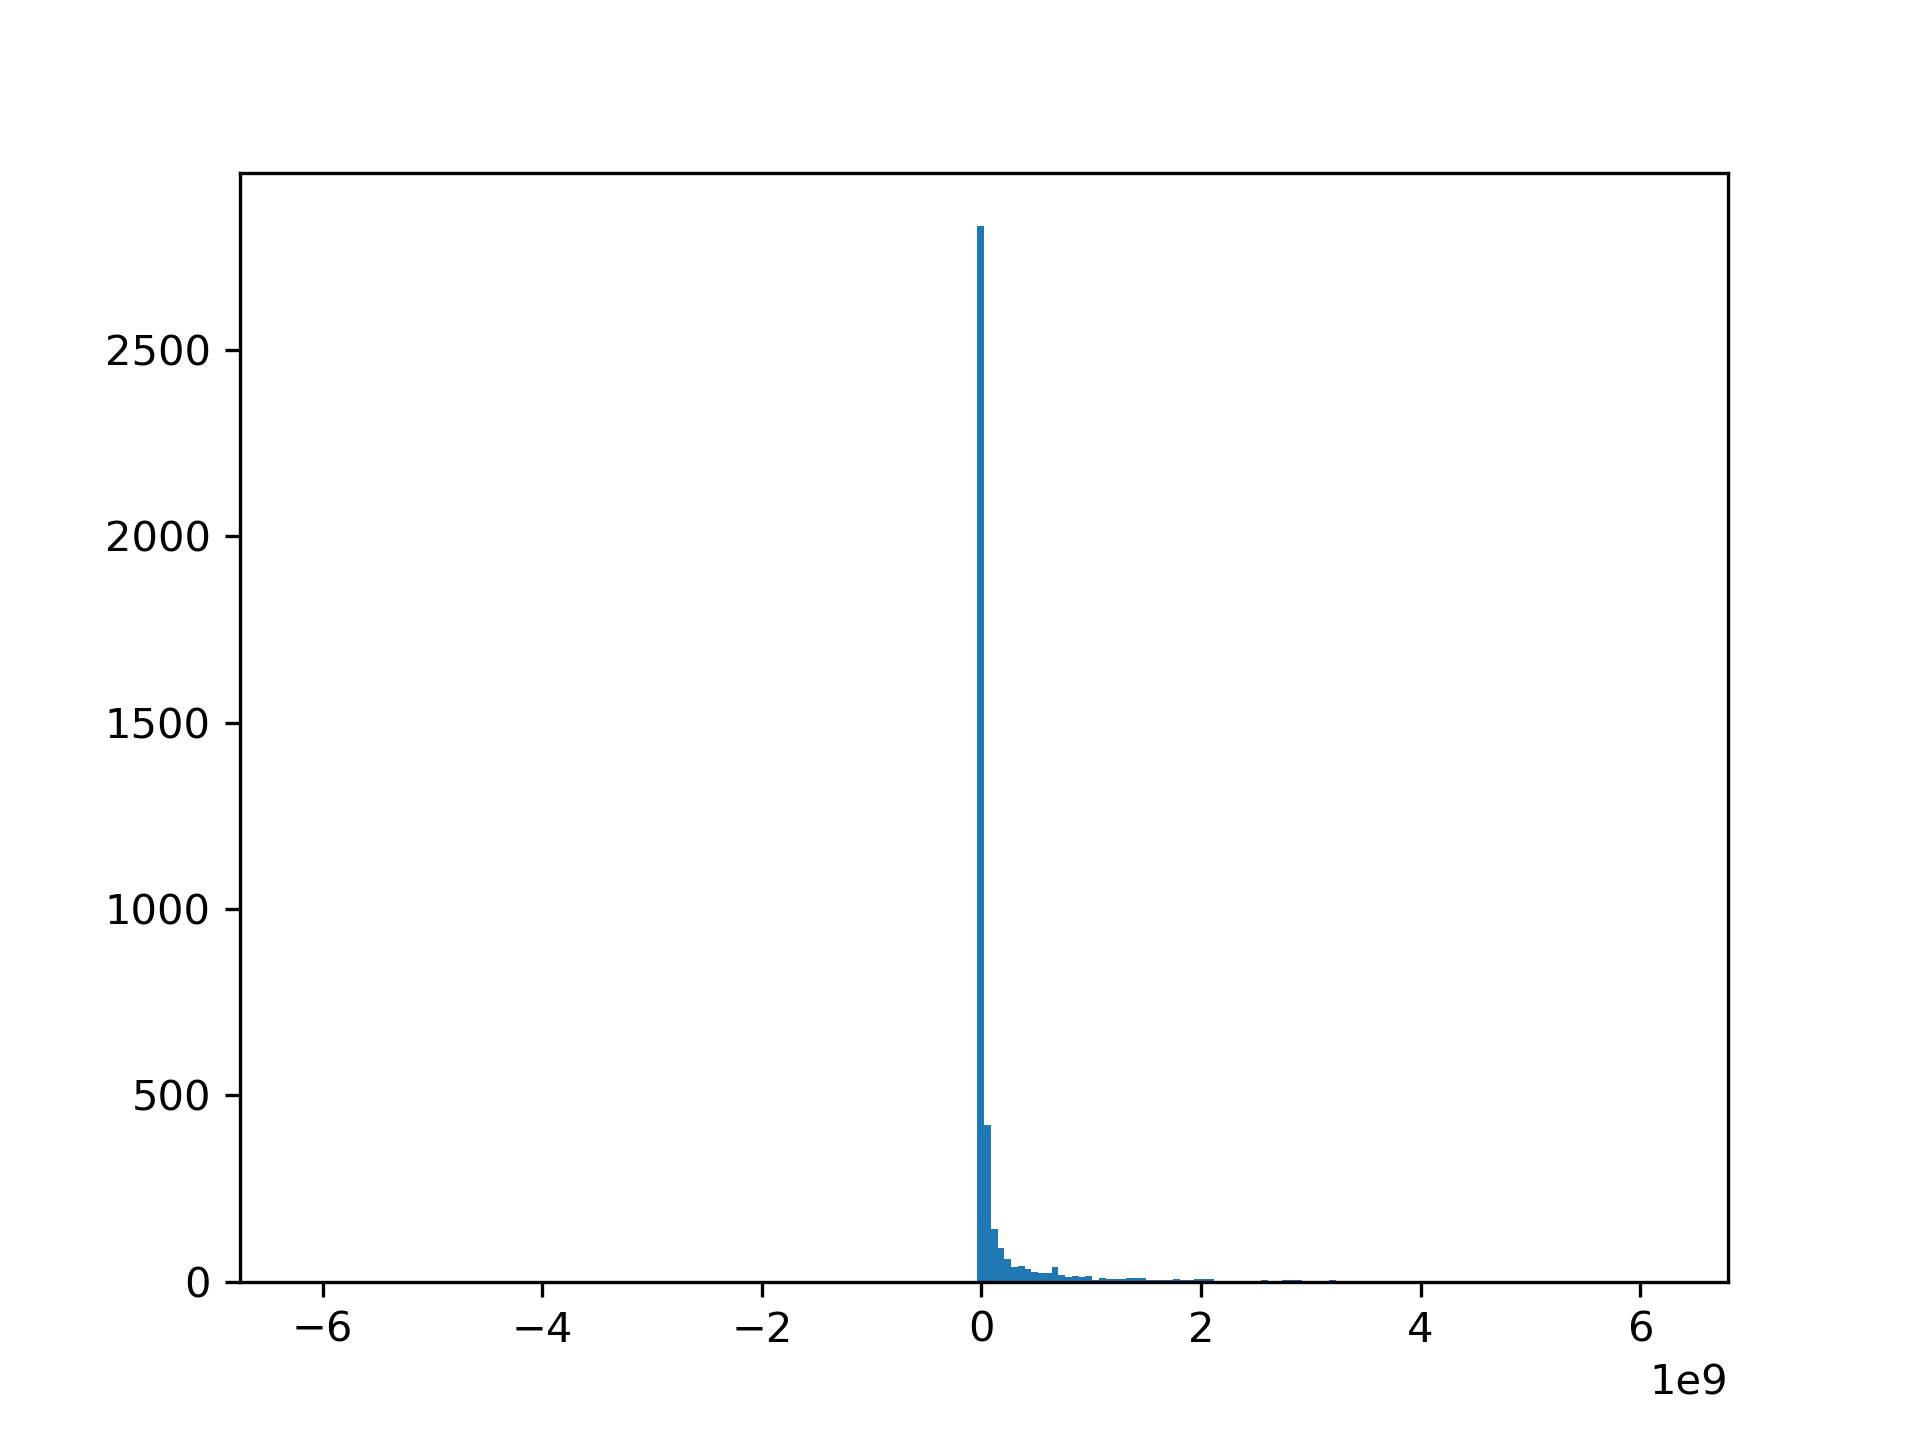
\includegraphics[width=\linewidth]{variables/Short-term debt.png}
    \caption{Histogram Short-term debt }
\end{figure}\section{ Total current liabilities }

\begin{center}
    \begin{tabular}{|c | c|} 
    \hline
    Statystyka & Wartość \\
    \hline\hline
    Średnia arytmetyczna & 9027882609.905437 \\ 
    \hline
    Odchylenie standardowe & 86793026823.20143 \\
    \hline
    Kwartyl dolny & 36943945.730825 \\
    \hline
    Mediana & 216228000.0 \\
    \hline
    Kwartyl górny & 1210531750.0 \\
    \hline
    Wartość najmniejsza & -21077918781.7259 \\
    \hline
    Wartość największa & 2095310000000.0 \\
    \hline
   \end{tabular}
\end{center}

\begin{figure}[h!]
    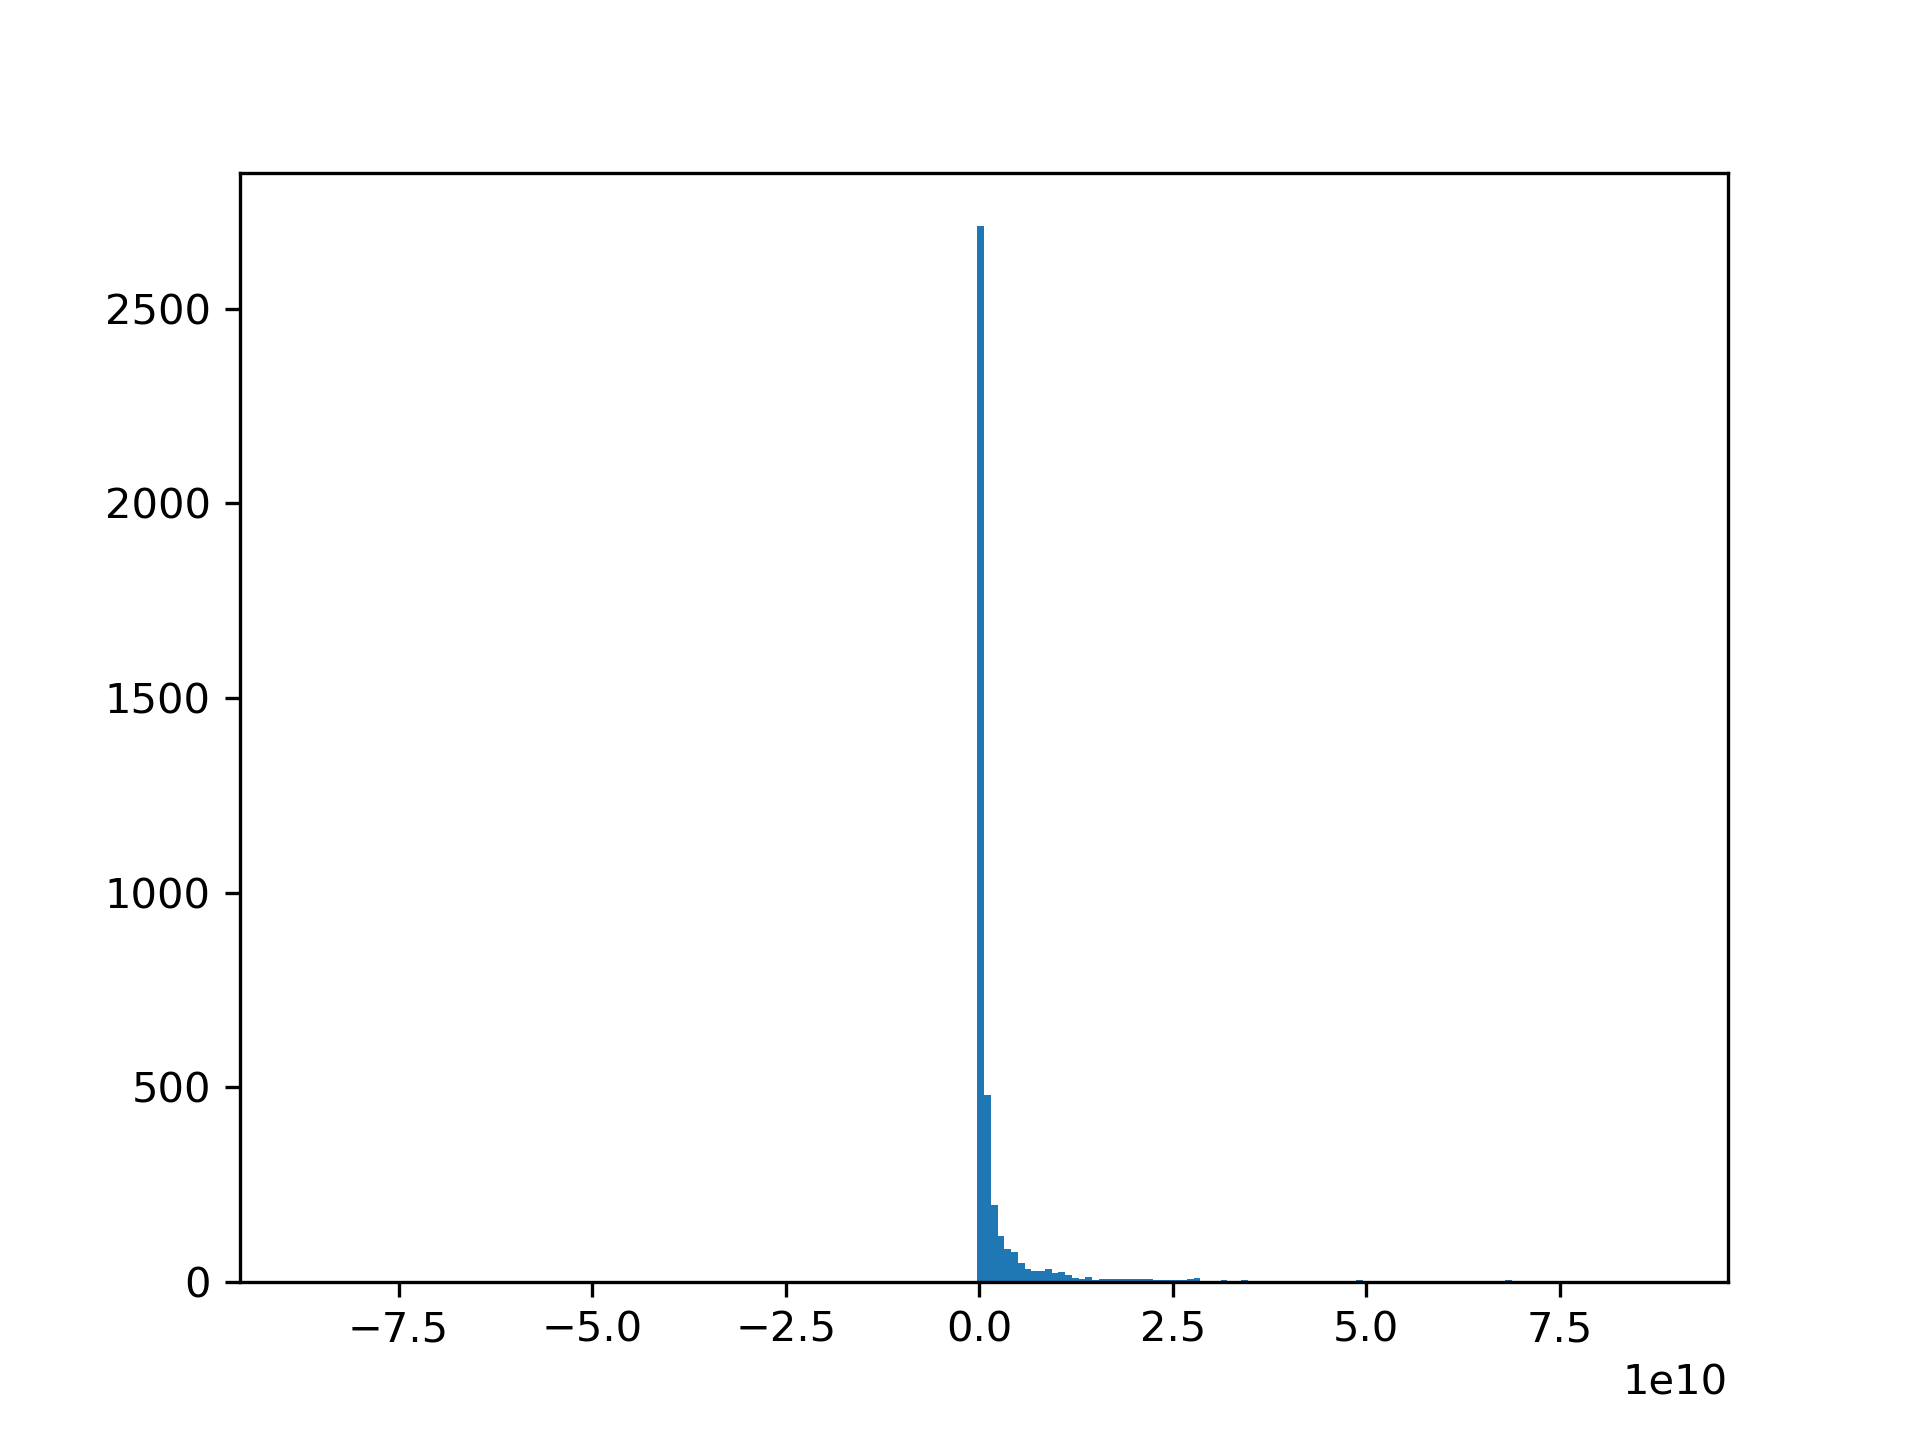
\includegraphics[width=\linewidth]{variables/Total current liabilities.png}
    \caption{Histogram Total current liabilities }
\end{figure}\section{ Long-term debt }

\begin{center}
    \begin{tabular}{|c | c|} 
    \hline
    Statystyka & Wartość \\
    \hline\hline
    Średnia arytmetyczna & 3244656772.897551 \\ 
    \hline
    Odchylenie standardowe & 17589332074.030334 \\
    \hline
    Kwartyl dolny & 2254848.25 \\
    \hline
    Mediana & 190791000.0 \\
    \hline
    Kwartyl górny & 1413664000.0 \\
    \hline
    Wartość najmniejsza & -7150761421.3198 \\
    \hline
    Wartość największa & 733000000000.0 \\
    \hline
   \end{tabular}
\end{center}

\begin{figure}[h!]
    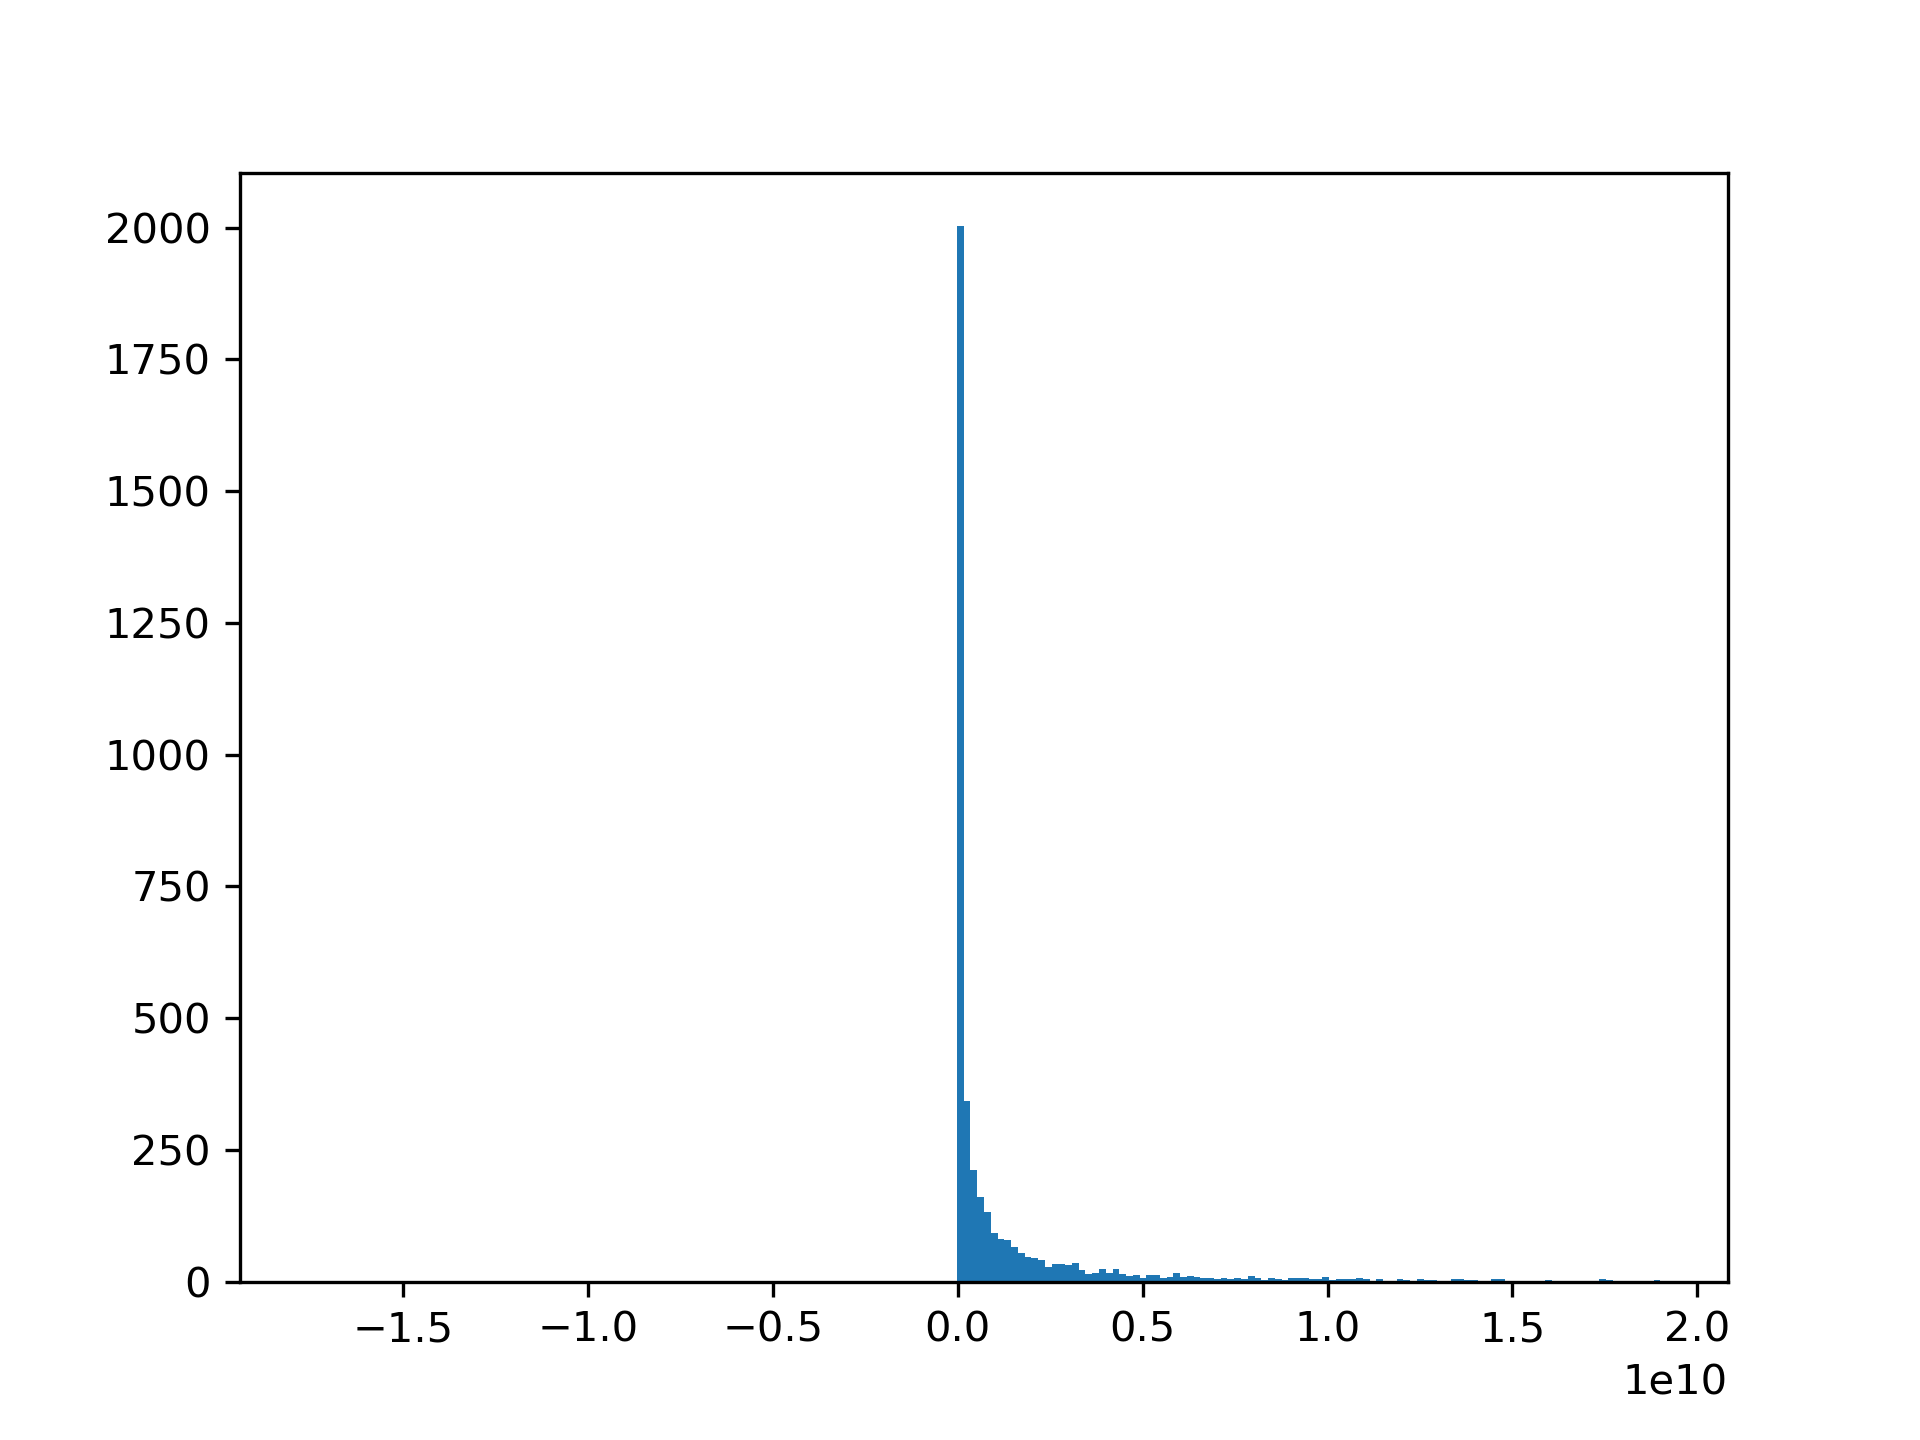
\includegraphics[width=\linewidth]{variables/Long-term debt.png}
    \caption{Histogram Long-term debt }
\end{figure}\section{ Total debt }

\begin{center}
    \begin{tabular}{|c | c|} 
    \hline
    Statystyka & Wartość \\
    \hline\hline
    Średnia arytmetyczna & 4214469657.847278 \\ 
    \hline
    Odchylenie standardowe & 23188130877.89325 \\
    \hline
    Kwartyl dolny & 9144750.0 \\
    \hline
    Mediana & 249832272.06945002 \\
    \hline
    Kwartyl górny & 1662443500.0 \\
    \hline
    Wartość najmniejsza & -8451649746.1929 \\
    \hline
    Wartość największa & 533627000000.0 \\
    \hline
   \end{tabular}
\end{center}

\begin{figure}[h!]
    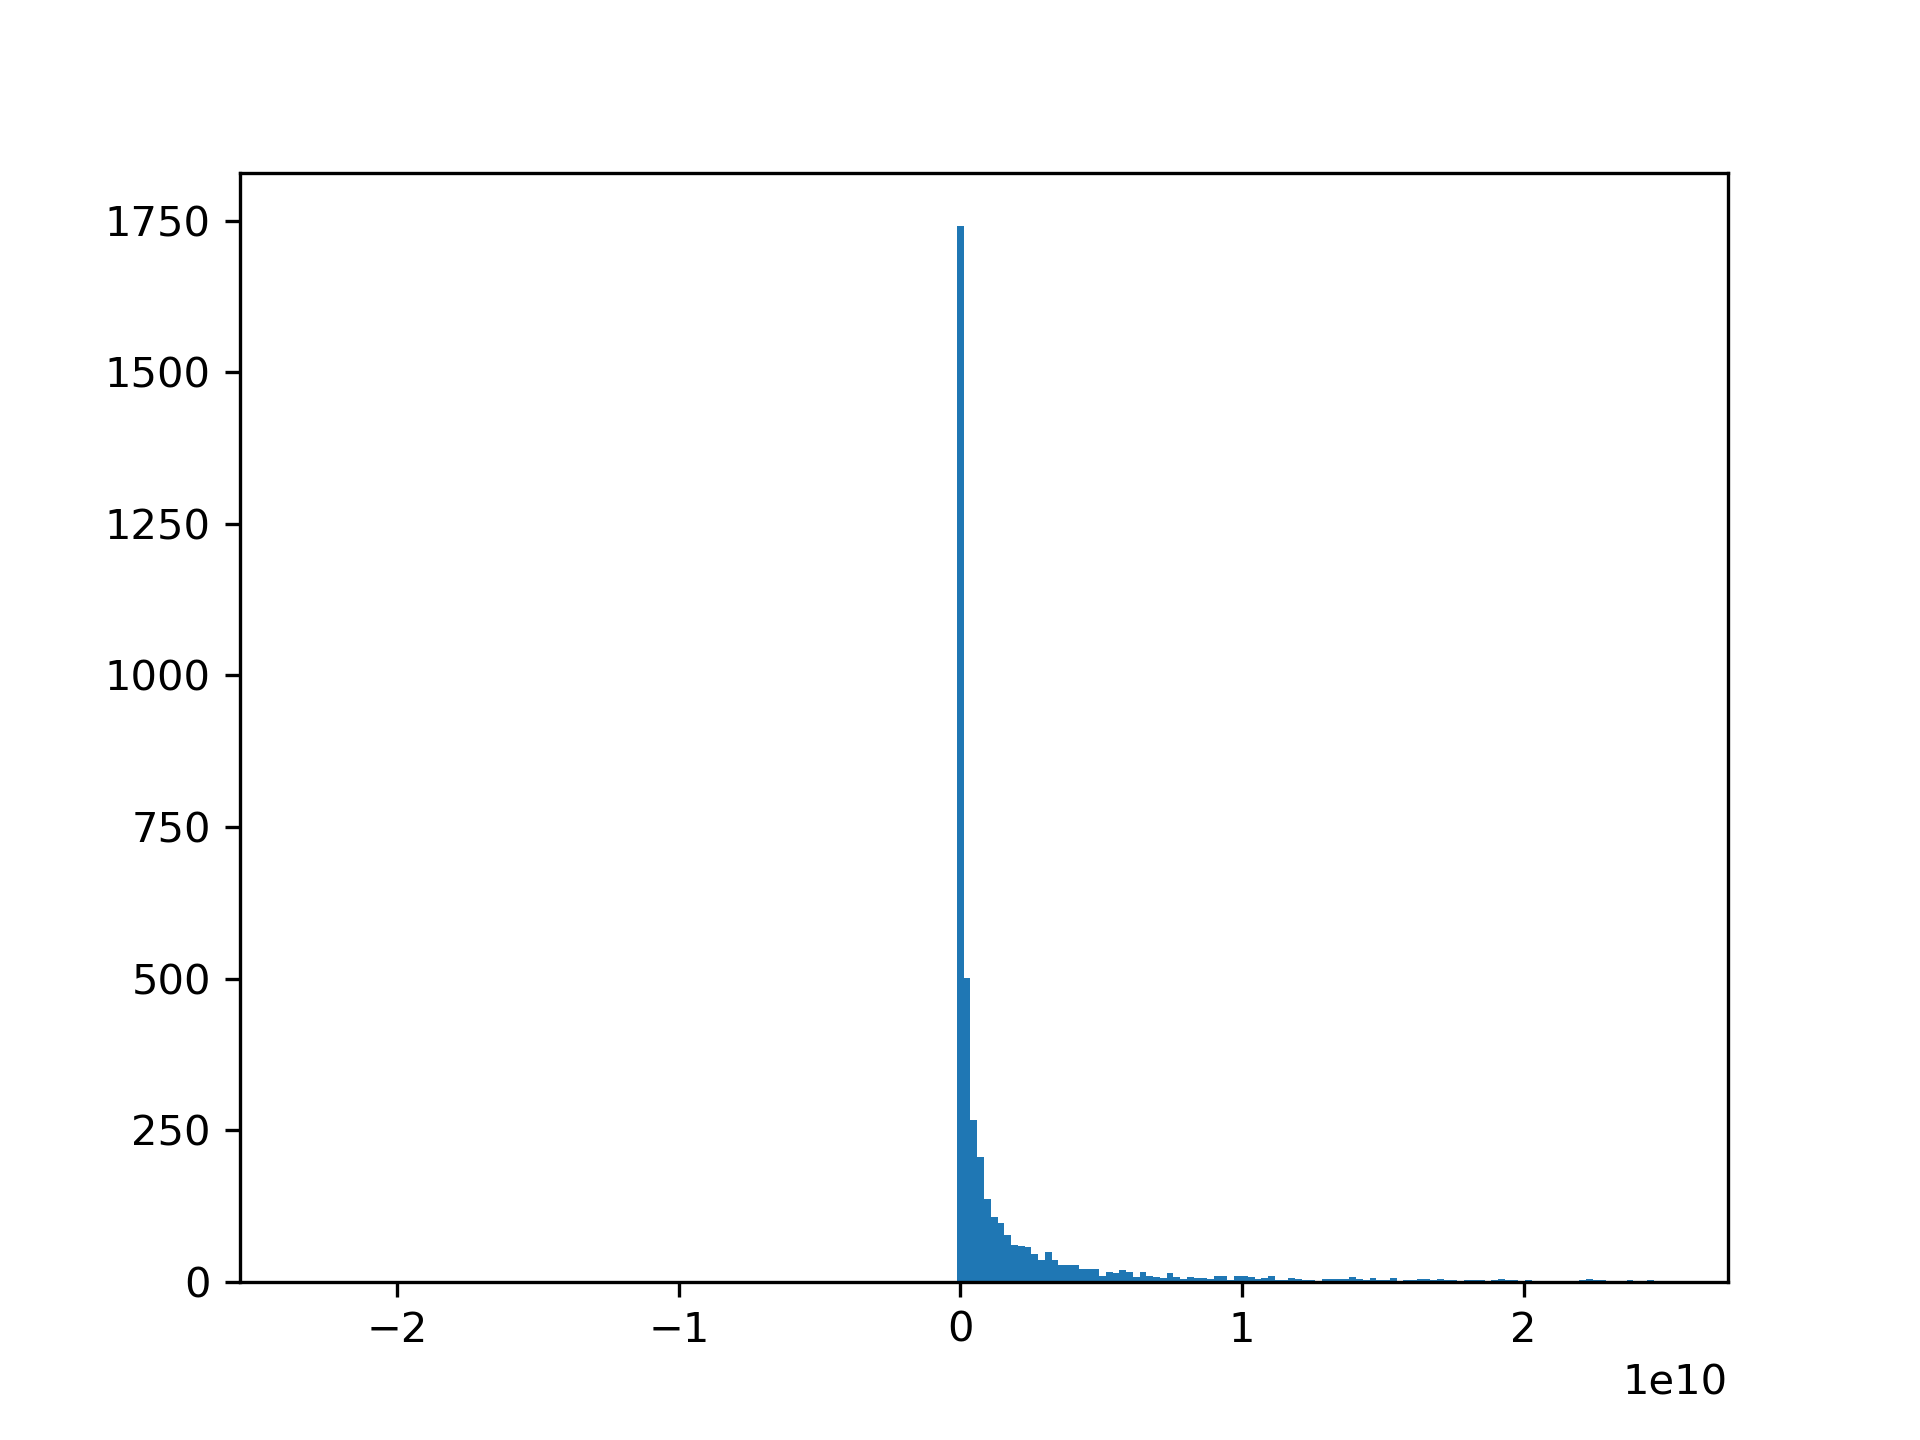
\includegraphics[width=\linewidth]{variables/Total debt.png}
    \caption{Histogram Total debt }
\end{figure}\section{ Deferred revenue }

\begin{center}
    \begin{tabular}{|c | c|} 
    \hline
    Statystyka & Wartość \\
    \hline\hline
    Średnia arytmetyczna & 141030975.87985685 \\ 
    \hline
    Odchylenie standardowe & 1288063108.2135615 \\
    \hline
    Kwartyl dolny & 0.0 \\
    \hline
    Mediana & 0.0 \\
    \hline
    Kwartyl górny & 3049750.0 \\
    \hline
    Wartość najmniejsza & 0.0 \\
    \hline
    Wartość największa & 50676000000.0 \\
    \hline
   \end{tabular}
\end{center}

\begin{figure}[h!]
    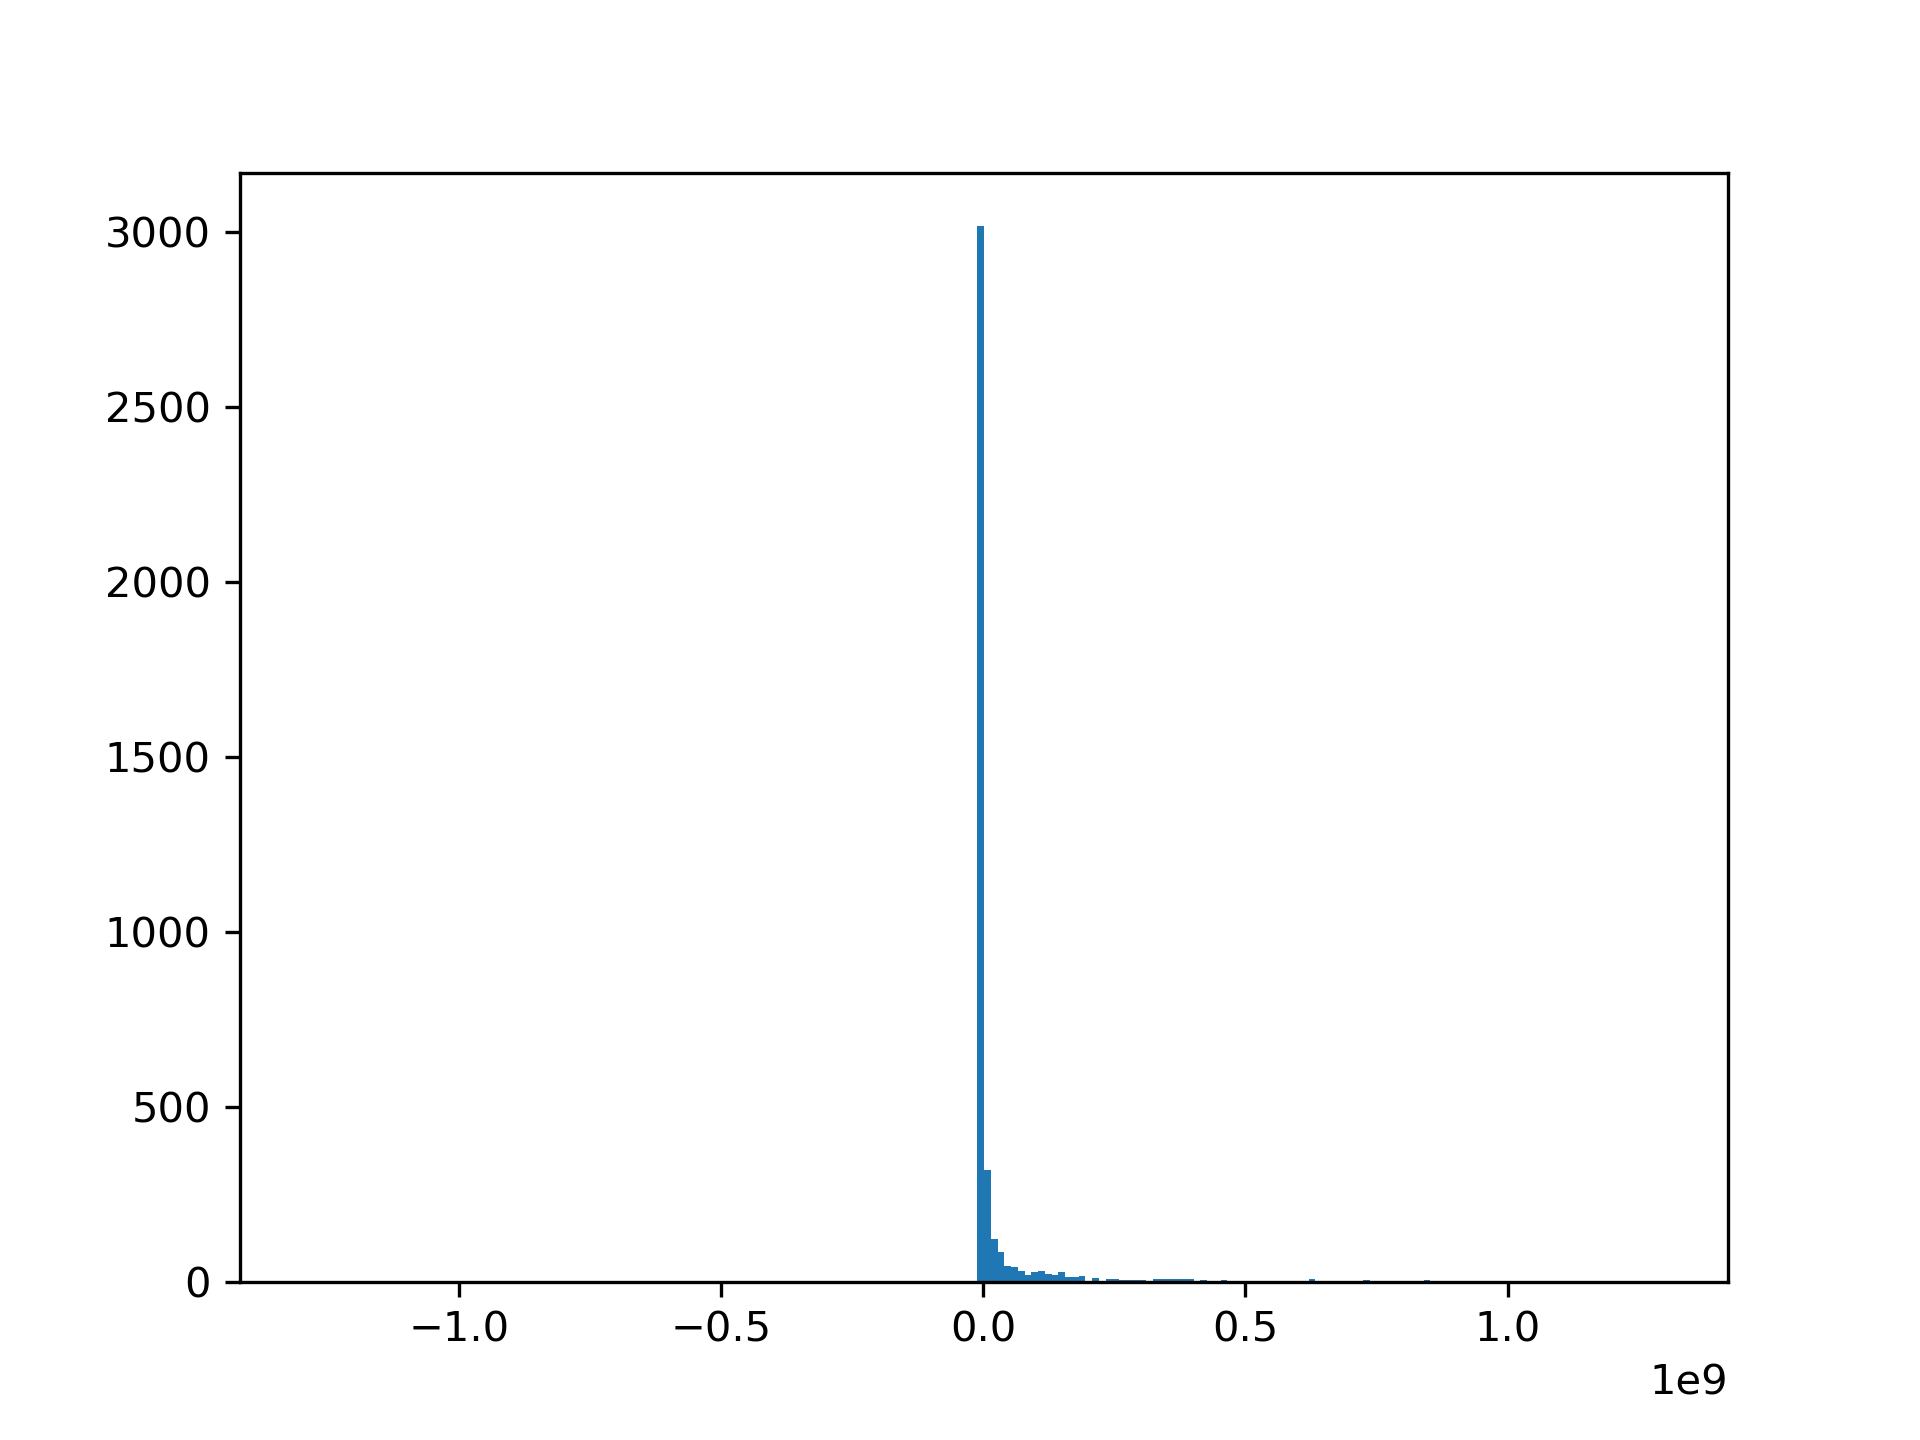
\includegraphics[width=\linewidth]{variables/Deferred revenue.png}
    \caption{Histogram Deferred revenue }
\end{figure}\section{ Tax Liabilities }

\begin{center}
    \begin{tabular}{|c | c|} 
    \hline
    Statystyka & Wartość \\
    \hline\hline
    Średnia arytmetyczna & 337989829.4200946 \\ 
    \hline
    Odchylenie standardowe & 1871325162.7814834 \\
    \hline
    Kwartyl dolny & 0.0 \\
    \hline
    Mediana & 252494.0 \\
    \hline
    Kwartyl górny & 52509750.0 \\
    \hline
    Wartość najmniejsza & -1301269035.533 \\
    \hline
    Wartość największa & 59038000000.0 \\
    \hline
   \end{tabular}
\end{center}

\begin{figure}[h!]
    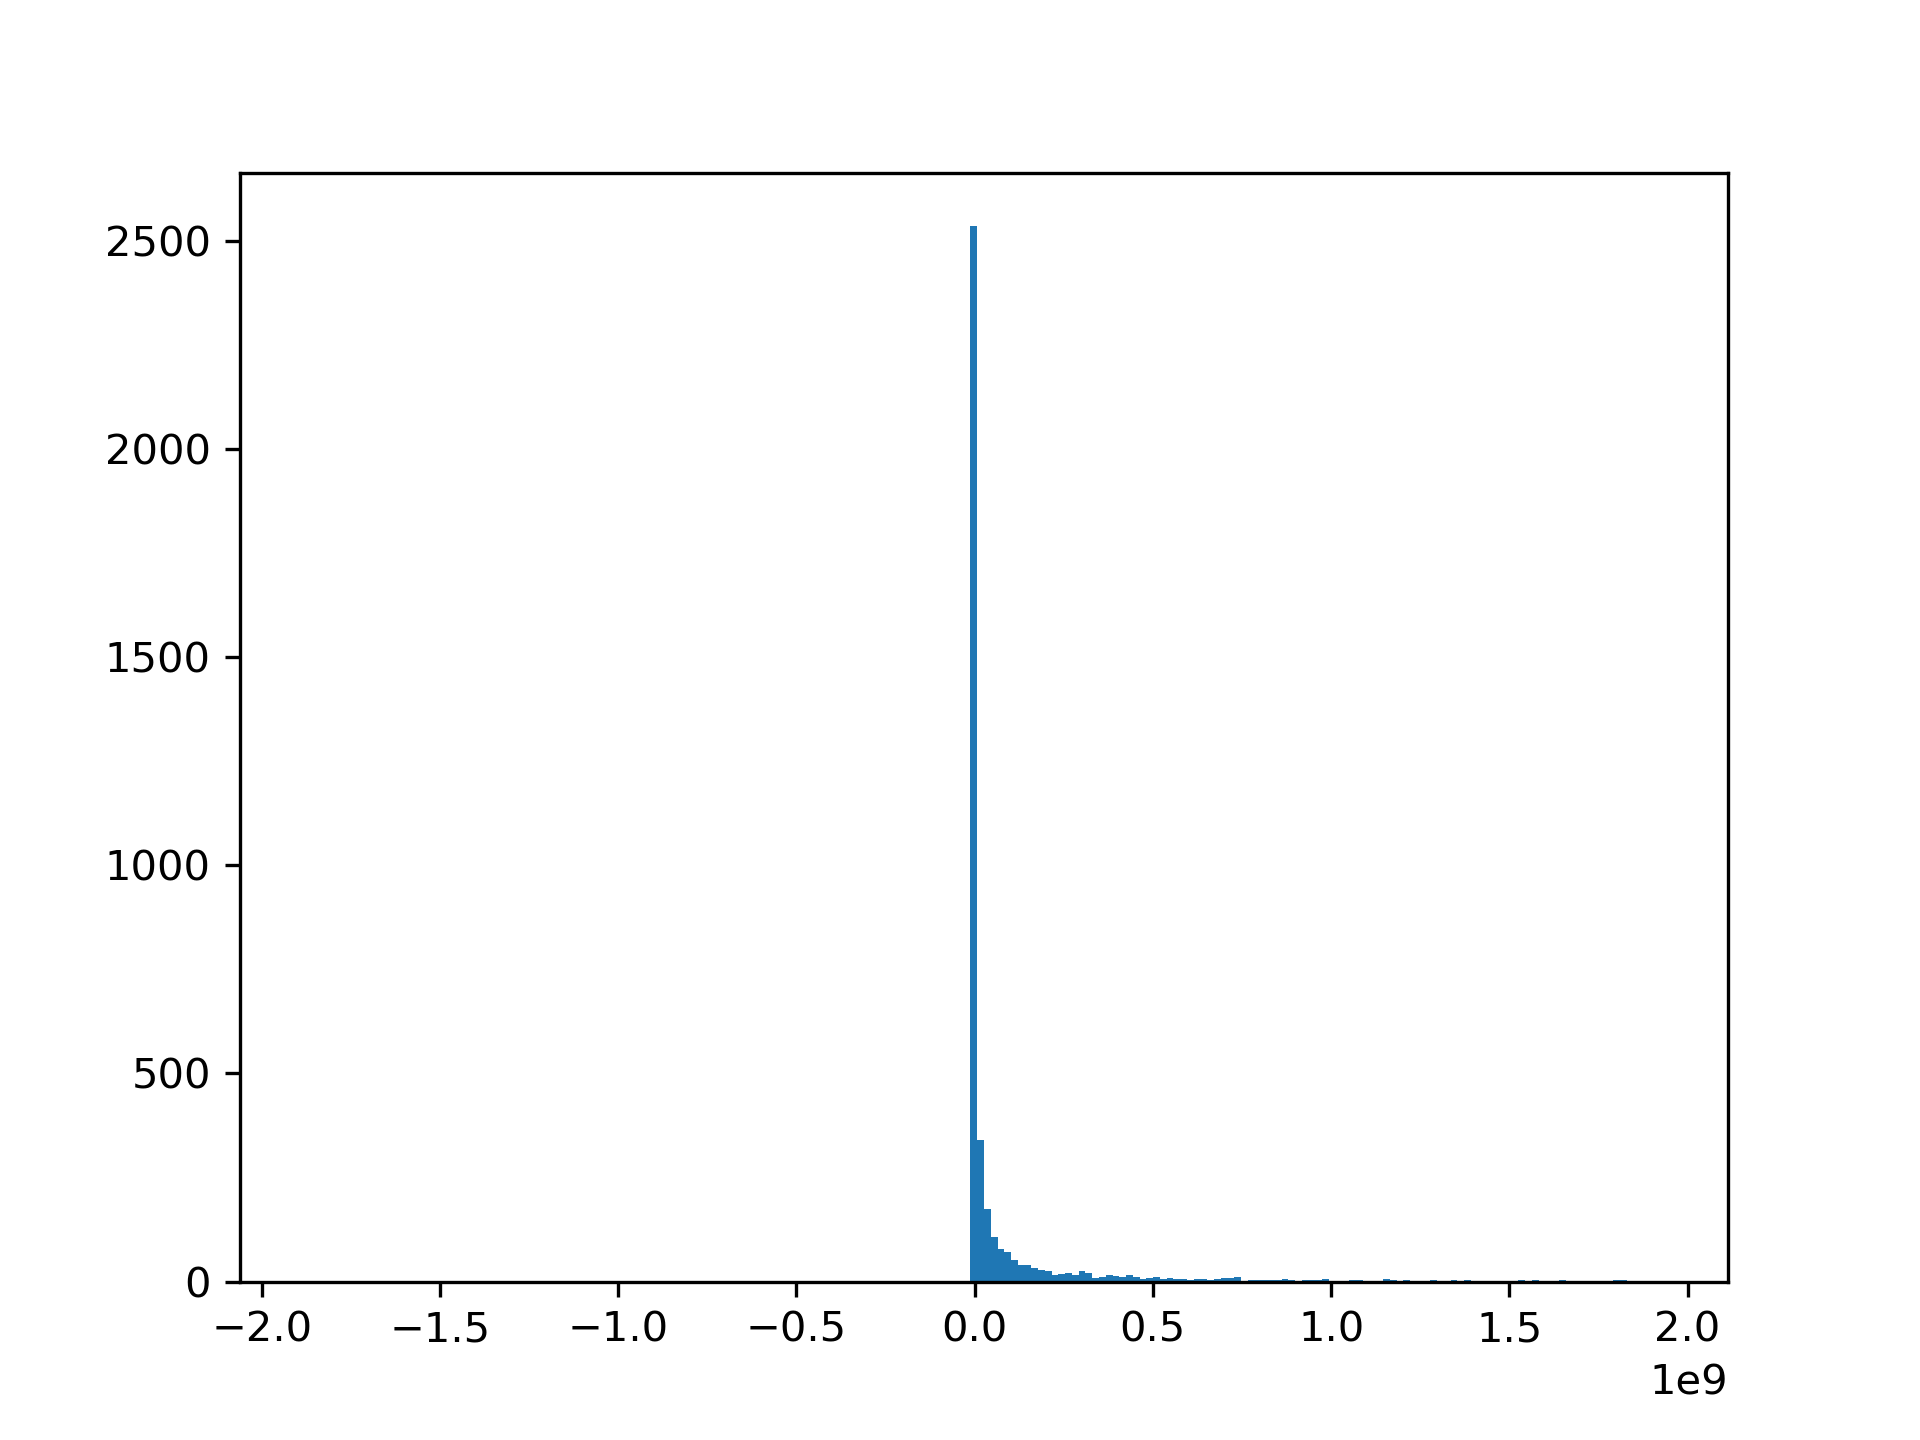
\includegraphics[width=\linewidth]{variables/Tax Liabilities.png}
    \caption{Histogram Tax Liabilities }
\end{figure}\section{ Deposit Liabilities }

\begin{center}
    \begin{tabular}{|c | c|} 
    \hline
    Statystyka & Wartość \\
    \hline\hline
    Średnia arytmetyczna & 5269104403.623925 \\ 
    \hline
    Odchylenie standardowe & 60748928614.97118 \\
    \hline
    Kwartyl dolny & 0.0 \\
    \hline
    Mediana & 0.0 \\
    \hline
    Kwartyl górny & 0.0 \\
    \hline
    Wartość najmniejsza & 0.0 \\
    \hline
    Wartość największa & 1470666000000.0 \\
    \hline
   \end{tabular}
\end{center}

\begin{figure}[h!]
    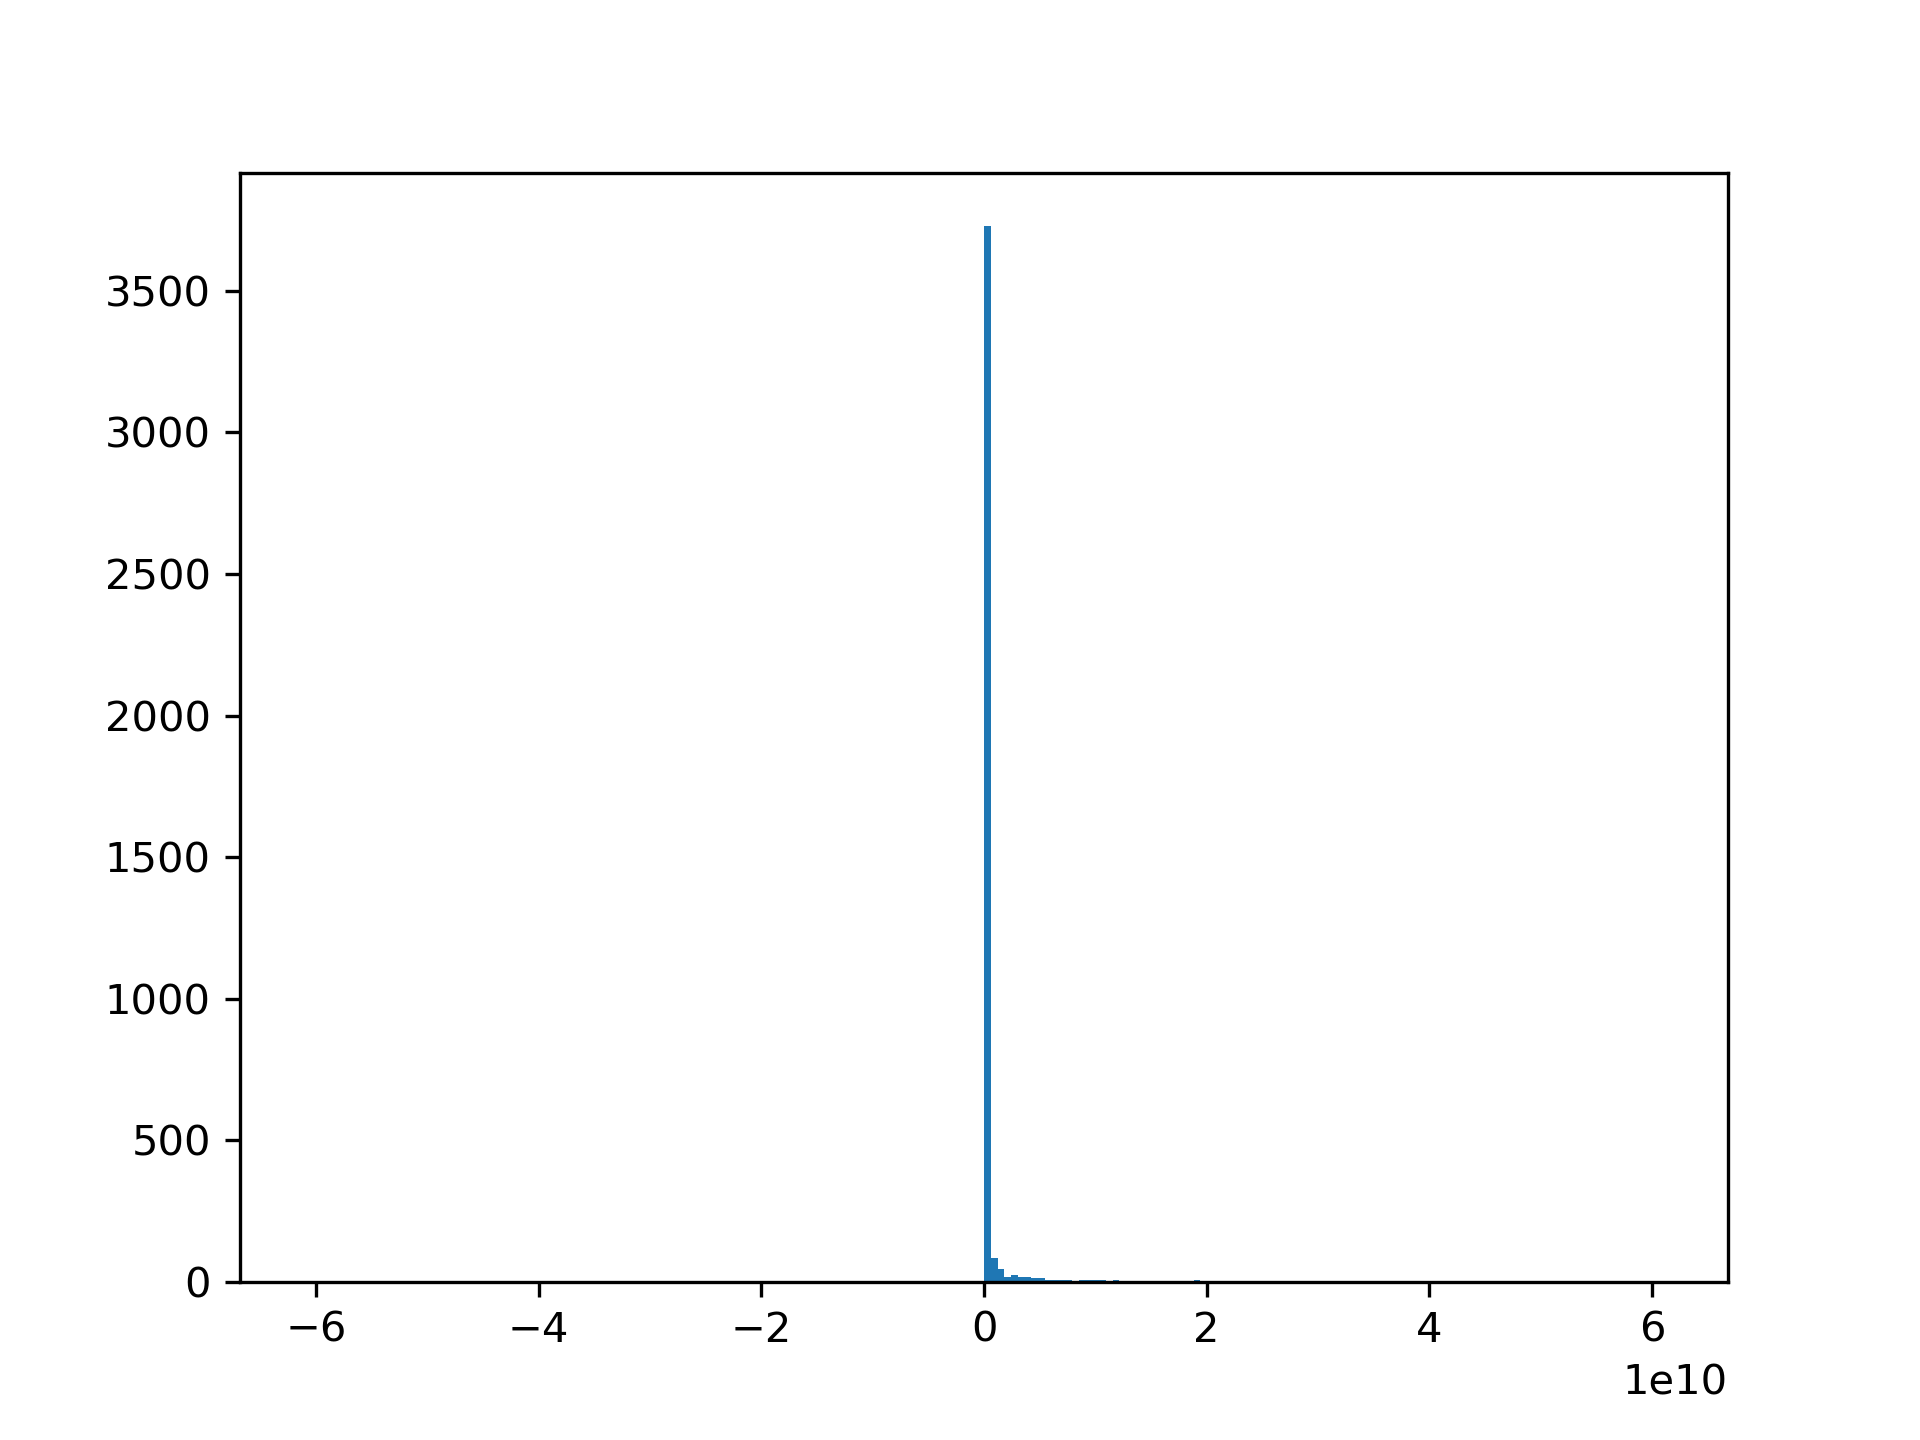
\includegraphics[width=\linewidth]{variables/Deposit Liabilities.png}
    \caption{Histogram Deposit Liabilities }
\end{figure}\section{ Total liabilities }

\begin{center}
    \begin{tabular}{|c | c|} 
    \hline
    Statystyka & Wartość \\
    \hline\hline
    Średnia arytmetyczna & 14732050994.791912 \\ 
    \hline
    Odchylenie standardowe & 103129713658.74908 \\
    \hline
    Kwartyl dolny & 93381750.0 \\
    \hline
    Mediana & 728061000.0 \\
    \hline
    Kwartyl górny & 3642571000.0 \\
    \hline
    Wartość najmniejsza & -7872214182.3444 \\
    \hline
    Wartość największa & 2366017000000.0 \\
    \hline
   \end{tabular}
\end{center}

\begin{figure}[h!]
    \includegraphics[width=\linewidth]{variables/Total liabilities.png}
    \caption{Histogram Total liabilities }
\end{figure}\section{ Other comprehensive income }

\begin{center}
    \begin{tabular}{|c | c|} 
    \hline
    Statystyka & Wartość \\
    \hline\hline
    Średnia arytmetyczna & -185837479.00910142 \\ 
    \hline
    Odchylenie standardowe & 2088878315.448341 \\
    \hline
    Kwartyl dolny & -24841000.0 \\
    \hline
    Mediana & -608685.0 \\
    \hline
    Kwartyl górny & 0.0 \\
    \hline
    Wartość najmniejsza & -94785000000.0 \\
    \hline
    Wartość największa & 38779637377.9637 \\
    \hline
   \end{tabular}
\end{center}

\begin{figure}[h!]
    \includegraphics[width=\linewidth]{variables/Other comprehensive income.png}
    \caption{Histogram Other comprehensive income }
\end{figure}\section{ Retained earnings (deficit) }

\begin{center}
    \begin{tabular}{|c | c|} 
    \hline
    Statystyka & Wartość \\
    \hline\hline
    Średnia arytmetyczna & 2178060991.801141 \\ 
    \hline
    Odchylenie standardowe & 13104557400.679403 \\
    \hline
    Kwartyl dolny & -160387091.0 \\
    \hline
    Mediana & 27987500.0 \\
    \hline
    Kwartyl górny & 606830250.0 \\
    \hline
    Wartość najmniejsza & -148807531380.7531 \\
    \hline
    Wartość największa & 421653000000.0 \\
    \hline
   \end{tabular}
\end{center}

\begin{figure}[h!]
    \includegraphics[width=\linewidth]{variables/Retained earnings (deficit).png}
    \caption{Histogram Retained earnings (deficit) }
\end{figure}\section{ Total shareholders equity }

\begin{center}
    \begin{tabular}{|c | c|} 
    \hline
    Statystyka & Wartość \\
    \hline\hline
    Średnia arytmetyczna & 3496719560.0776734 \\ 
    \hline
    Odchylenie standardowe & 13817668581.458887 \\
    \hline
    Kwartyl dolny & 81144750.0 \\
    \hline
    Mediana & 410848500.0 \\
    \hline
    Kwartyl górny & 1690442250.0 \\
    \hline
    Wartość najmniejsza & -12459000000.0 \\
    \hline
    Wartość największa & 265325000000.0 \\
    \hline
   \end{tabular}
\end{center}

\begin{figure}[h!]
    \includegraphics[width=\linewidth]{variables/Total shareholders equity.png}
    \caption{Histogram Total shareholders equity }
\end{figure}\section{ Investments }

\begin{center}
    \begin{tabular}{|c | c|} 
    \hline
    Statystyka & Wartość \\
    \hline\hline
    Średnia arytmetyczna & 9085795393.337812 \\ 
    \hline
    Odchylenie standardowe & 83913412998.3199 \\
    \hline
    Kwartyl dolny & 0.0 \\
    \hline
    Mediana & 15000000.0 \\
    \hline
    Kwartyl górny & 424084500.0 \\
    \hline
    Wartość najmniejsza & -110248000.0 \\
    \hline
    Wartość największa & 2080234000000.0 \\
    \hline
   \end{tabular}
\end{center}

\begin{figure}[h!]
    \includegraphics[width=\linewidth]{variables/Investments.png}
    \caption{Histogram Investments }
\end{figure}\section{ Net Debt }

\begin{center}
    \begin{tabular}{|c | c|} 
    \hline
    Statystyka & Wartość \\
    \hline\hline
    Średnia arytmetyczna & 1156981480.106203 \\ 
    \hline
    Odchylenie standardowe & 21742604825.077454 \\
    \hline
    Kwartyl dolny & -36441250.0 \\
    \hline
    Mediana & 61426000.0 \\
    \hline
    Kwartyl górny & 1156981480.1062033 \\
    \hline
    Wartość najmniejsza & -444365000000.0 \\
    \hline
    Wartość największa & 731102232000.0 \\
    \hline
   \end{tabular}
\end{center}

\begin{figure}[h!]
    \includegraphics[width=\linewidth]{variables/Net Debt.png}
    \caption{Histogram Net Debt }
\end{figure}\section{ Other Assets }

\begin{center}
    \begin{tabular}{|c | c|} 
    \hline
    Statystyka & Wartość \\
    \hline\hline
    Średnia arytmetyczna & 1399658462.8513148 \\ 
    \hline
    Odchylenie standardowe & 28659561806.24284 \\
    \hline
    Kwartyl dolny & 2511000.0 \\
    \hline
    Mediana & 19802500.0 \\
    \hline
    Kwartyl górny & 118216750.0 \\
    \hline
    Wartość najmniejsza & -911986573000.0 \\
    \hline
    Wartość największa & 601019683151.3256 \\
    \hline
   \end{tabular}
\end{center}

\begin{figure}[h!]
    \includegraphics[width=\linewidth]{variables/Other Assets.png}
    \caption{Histogram Other Assets }
\end{figure}\section{ Other Liabilities }

\begin{center}
    \begin{tabular}{|c | c|} 
    \hline
    Statystyka & Wartość \\
    \hline\hline
    Średnia arytmetyczna & 7448344114.5233 \\ 
    \hline
    Odchylenie standardowe & 80816975735.51486 \\
    \hline
    Kwartyl dolny & 10546500.0 \\
    \hline
    Mediana & 78931500.0 \\
    \hline
    Kwartyl górny & 561549500.0 \\
    \hline
    Wartość najmniejsza & -61946000000.0 \\
    \hline
    Wartość największa & 1866206000000.0 \\
    \hline
   \end{tabular}
\end{center}

\begin{figure}[h!]
    \includegraphics[width=\linewidth]{variables/Other Liabilities.png}
    \caption{Histogram Other Liabilities }
\end{figure}\section{ Depreciation and Amortization }

\begin{center}
    \begin{tabular}{|c | c|} 
    \hline
    Statystyka & Wartość \\
    \hline\hline
    Średnia arytmetyczna & 302163314.27345514 \\ 
    \hline
    Odchylenie standardowe & 1347193487.154766 \\
    \hline
    Kwartyl dolny & 2421000.0 \\
    \hline
    Mediana & 24196000.0 \\
    \hline
    Kwartyl górny & 136315000.0 \\
    \hline
    Wartość najmniejsza & -25184000.0 \\
    \hline
    Wartość największa & 33564254703.3285 \\
    \hline
   \end{tabular}
\end{center}

\begin{figure}[h!]
    \includegraphics[width=\linewidth]{variables/Depreciation _ Amortization.png}
    \caption{Histogram Depreciation and Amortization }
\end{figure}\section{ Stock-based compensation }

\begin{center}
    \begin{tabular}{|c | c|} 
    \hline
    Statystyka & Wartość \\
    \hline\hline
    Średnia arytmetyczna & 35087760.93374329 \\ 
    \hline
    Odchylenie standardowe & 235473531.6574922 \\
    \hline
    Kwartyl dolny & 680750.0 \\
    \hline
    Mediana & 4959500.0 \\
    \hline
    Kwartyl górny & 18325250.0 \\
    \hline
    Wartość najmniejsza & -108148148.1481 \\
    \hline
    Wartość największa & 9353000000.0 \\
    \hline
   \end{tabular}
\end{center}

\begin{figure}[h!]
    \includegraphics[width=\linewidth]{variables/Stock-based compensation.png}
    \caption{Histogram Stock-based compensation }
\end{figure}\section{ Operating Cash Flow }

\begin{center}
    \begin{tabular}{|c | c|} 
    \hline
    Statystyka & Wartość \\
    \hline\hline
    Średnia arytmetyczna & 848459804.751946 \\ 
    \hline
    Odchylenie standardowe & 3905164402.7226787 \\
    \hline
    Kwartyl dolny & 789250.0 \\
    \hline
    Mediana & 69810000.0 \\
    \hline
    Kwartyl górny & 389914250.0 \\
    \hline
    Wartość najmniejsza & -62144827586.2069 \\
    \hline
    Wartość największa & 97722096847.5561 \\
    \hline
   \end{tabular}
\end{center}

\begin{figure}[h!]
    \includegraphics[width=\linewidth]{variables/Operating Cash Flow.png}
    \caption{Histogram Operating Cash Flow }
\end{figure}\section{ Capital Expenditure }

\begin{center}
    \begin{tabular}{|c | c|} 
    \hline
    Statystyka & Wartość \\
    \hline\hline
    Średnia arytmetyczna & -344195749.17435336 \\ 
    \hline
    Odchylenie standardowe & 1516019313.288606 \\
    \hline
    Kwartyl dolny & -135251500.0 \\
    \hline
    Mediana & -19212000.0 \\
    \hline
    Kwartyl górny & -1433750.0 \\
    \hline
    Wartość najmniejsza & -38437626628.0753 \\
    \hline
    Wartość największa & 1459699000.0 \\
    \hline
   \end{tabular}
\end{center}

\begin{figure}[h!]
    \includegraphics[width=\linewidth]{variables/Capital Expenditure.png}
    \caption{Histogram Capital Expenditure }
\end{figure}\section{ Acquisitions and disposals }

\begin{center}
    \begin{tabular}{|c | c|} 
    \hline
    Statystyka & Wartość \\
    \hline\hline
    Średnia arytmetyczna & -134076339.05268759 \\ 
    \hline
    Odchylenie standardowe & 1442857422.4142635 \\
    \hline
    Kwartyl dolny & -14187000.0 \\
    \hline
    Mediana & 0.0 \\
    \hline
    Kwartyl górny & 0.0 \\
    \hline
    Wartość najmniejsza & -41711000000.0 \\
    \hline
    Wartość największa & 8823000000.0 \\
    \hline
   \end{tabular}
\end{center}

\begin{figure}[h!]
    \includegraphics[width=\linewidth]{variables/Acquisitions and disposals.png}
    \caption{Histogram Acquisitions and disposals }
\end{figure}\section{ Investment purchases and sales }

\begin{center}
    \begin{tabular}{|c | c|} 
    \hline
    Statystyka & Wartość \\
    \hline\hline
    Średnia arytmetyczna & -192265134.8640731 \\ 
    \hline
    Odchylenie standardowe & 4789956641.275278 \\
    \hline
    Kwartyl dolny & -9618250.0 \\
    \hline
    Mediana & 0.0 \\
    \hline
    Kwartyl górny & 0.0 \\
    \hline
    Wartość najmniejsza & -193007000000.0 \\
    \hline
    Wartość największa & 119962693747.5946 \\
    \hline
   \end{tabular}
\end{center}

\begin{figure}[h!]
    \includegraphics[width=\linewidth]{variables/Investment purchases and sales.png}
    \caption{Histogram Investment purchases and sales }
\end{figure}\section{ Investing Cash flow }

\begin{center}
    \begin{tabular}{|c | c|} 
    \hline
    Statystyka & Wartość \\
    \hline\hline
    Średnia arytmetyczna & -661817765.9605068 \\ 
    \hline
    Odchylenie standardowe & 4569799319.747789 \\
    \hline
    Kwartyl dolny & -284946250.0 \\
    \hline
    Mediana & -47847000.0 \\
    \hline
    Kwartyl górny & -1375956.2901249998 \\
    \hline
    Wartość najmniejsza & -197993000000.0 \\
    \hline
    Wartość największa & 27533863779.3153 \\
    \hline
   \end{tabular}
\end{center}

\begin{figure}[h!]
    \includegraphics[width=\linewidth]{variables/Investing Cash flow.png}
    \caption{Histogram Investing Cash flow }
\end{figure}\section{ Issuance (repayment) of debt }

\begin{center}
    \begin{tabular}{|c | c|} 
    \hline
    Statystyka & Wartość \\
    \hline\hline
    Średnia arytmetyczna & 85343030.6086618 \\ 
    \hline
    Odchylenie standardowe & 1900652122.9477098 \\
    \hline
    Kwartyl dolny & -19583859.25 \\
    \hline
    Mediana & 0.0 \\
    \hline
    Kwartyl górny & 39760000.0 \\
    \hline
    Wartość najmniejsza & -44798850574.7126 \\
    \hline
    Wartość największa & 38265000000.0 \\
    \hline
   \end{tabular}
\end{center}

\begin{figure}[h!]
    \includegraphics[width=\linewidth]{variables/Issuance (repayment) of debt.png}
    \caption{Histogram Issuance (repayment) of debt }
\end{figure}\section{ Issuance (buybacks) of shares }

\begin{center}
    \begin{tabular}{|c | c|} 
    \hline
    Statystyka & Wartość \\
    \hline\hline
    Średnia arytmetyczna & -183692056.2289874 \\ 
    \hline
    Odchylenie standardowe & 1590188048.1127787 \\
    \hline
    Kwartyl dolny & -17544000.0 \\
    \hline
    Mediana & 0.0 \\
    \hline
    Kwartyl górny & 5258094.75 \\
    \hline
    Wartość najmniejsza & -72069000000.0 \\
    \hline
    Wartość największa & 4136000000.0 \\
    \hline
   \end{tabular}
\end{center}

\begin{figure}[h!]
    \includegraphics[width=\linewidth]{variables/Issuance (buybacks) of shares.png}
    \caption{Histogram Issuance (buybacks) of shares }
\end{figure}\section{ Dividend payments }

\begin{center}
    \begin{tabular}{|c | c|} 
    \hline
    Statystyka & Wartość \\
    \hline\hline
    Średnia arytmetyczna & -202388624.86748907 \\ 
    \hline
    Odchylenie standardowe & 879844491.9679061 \\
    \hline
    Kwartyl dolny & -55548000.0 \\
    \hline
    Mediana & 0.0 \\
    \hline
    Kwartyl górny & 0.0 \\
    \hline
    Wartość najmniejsza & -13798000000.0 \\
    \hline
    Wartość największa & 0.0 \\
    \hline
   \end{tabular}
\end{center}

\begin{figure}[h!]
    \includegraphics[width=\linewidth]{variables/Dividend payments.png}
    \caption{Histogram Dividend payments }
\end{figure}\section{ Financing Cash Flow }

\begin{center}
    \begin{tabular}{|c | c|} 
    \hline
    Statystyka & Wartość \\
    \hline\hline
    Średnia arytmetyczna & -148638816.23589492 \\ 
    \hline
    Odchylenie standardowe & 4902118684.378467 \\
    \hline
    Kwartyl dolny & -119313750.0 \\
    \hline
    Mediana & -941305.94255 \\
    \hline
    Kwartyl górny & 47362750.0 \\
    \hline
    Wartość najmniejsza & -87876000000.0 \\
    \hline
    Wartość największa & 226000000000.0 \\
    \hline
   \end{tabular}
\end{center}

\begin{figure}[h!]
    \includegraphics[width=\linewidth]{variables/Financing Cash Flow.png}
    \caption{Histogram Financing Cash Flow }
\end{figure}\section{ Effect of forex changes on cash }

\begin{center}
    \begin{tabular}{|c | c|} 
    \hline
    Statystyka & Wartość \\
    \hline\hline
    Średnia arytmetyczna & -6334378.210097768 \\ 
    \hline
    Odchylenie standardowe & 114914063.93455079 \\
    \hline
    Kwartyl dolny & -494046.2963 \\
    \hline
    Mediana & 0.0 \\
    \hline
    Kwartyl górny & 0.0 \\
    \hline
    Wartość najmniejsza & -4000000000.0 \\
    \hline
    Wartość największa & 1917241379.3103 \\
    \hline
   \end{tabular}
\end{center}

\begin{figure}[h!]
    \includegraphics[width=\linewidth]{variables/Effect of forex changes on cash.png}
    \caption{Histogram Effect of forex changes on cash }
\end{figure}\section{ Net cash flow / Change in cash }

\begin{center}
    \begin{tabular}{|c | c|} 
    \hline
    Statystyka & Wartość \\
    \hline\hline
    Średnia arytmetyczna & -44110756.25468117 \\ 
    \hline
    Odchylenie standardowe & 3158691122.452035 \\
    \hline
    Kwartyl dolny & -24216000.0 \\
    \hline
    Mediana & 84682.0 \\
    \hline
    Kwartyl górny & 25082500.0 \\
    \hline
    Wartość najmniejsza & -152511000000.0 \\
    \hline
    Wartość największa & 62730808929.0088 \\
    \hline
   \end{tabular}
\end{center}

\begin{figure}[h!]
    \includegraphics[width=\linewidth]{variables/Net cash flow _ Change in cash.png}
    \caption{Histogram Net cash flow / Change in cash }
\end{figure}\section{ Free Cash Flow }

\begin{center}
    \begin{tabular}{|c | c|} 
    \hline
    Statystyka & Wartość \\
    \hline\hline
    Średnia arytmetyczna & 505001137.5332326 \\ 
    \hline
    Odchylenie standardowe & 3038980693.687234 \\
    \hline
    Kwartyl dolny & -10772362.0 \\
    \hline
    Mediana & 25180500.0 \\
    \hline
    Kwartyl górny & 209416385.5 \\
    \hline
    Wartość najmniejsza & -62270114942.5287 \\
    \hline
    Wartość największa & 94146198523.4946 \\
    \hline
   \end{tabular}
\end{center}

\begin{figure}[h!]
    \includegraphics[width=\linewidth]{variables/Free Cash Flow.png}
    \caption{Histogram Free Cash Flow }
\end{figure}\section{ Net Cash/Marketcap }

\begin{center}
    \begin{tabular}{|c | c|} 
    \hline
    Statystyka & Wartość \\
    \hline\hline
    Średnia arytmetyczna & -0.5845171039094651 \\ 
    \hline
    Odchylenie standardowe & 9.7278079690599 \\
    \hline
    Kwartyl dolny & -0.584517103909465 \\
    \hline
    Mediana & -0.1288 \\
    \hline
    Kwartyl górny & 0.0989 \\
    \hline
    Wartość najmniejsza & -210.7294 \\
    \hline
    Wartość największa & 501.7801 \\
    \hline
   \end{tabular}
\end{center}

\begin{figure}[h!]
    \includegraphics[width=\linewidth]{variables/Net Cash_Marketcap.png}
    \caption{Histogram Net Cash/Marketcap }
\end{figure}\section{ priceToSalesRatio }

\begin{center}
    \begin{tabular}{|c | c|} 
    \hline
    Statystyka & Wartość \\
    \hline\hline
    Średnia arytmetyczna & 22.834492429022085 \\ 
    \hline
    Odchylenie standardowe & 360.92625385137586 \\
    \hline
    Kwartyl dolny & 0.6254 \\
    \hline
    Mediana & 1.69645 \\
    \hline
    Kwartyl górny & 4.004575 \\
    \hline
    Wartość najmniejsza & 0.0 \\
    \hline
    Wartość największa & 15704.6886 \\
    \hline
   \end{tabular}
\end{center}

\begin{figure}[h!]
    \includegraphics[width=\linewidth]{variables/priceToSalesRatio.png}
    \caption{Histogram priceToSalesRatio }
\end{figure}\section{ priceEarningsRatio }

\begin{center}
    \begin{tabular}{|c | c|} 
    \hline
    Statystyka & Wartość \\
    \hline\hline
    Średnia arytmetyczna & 24.115413949539057 \\ 
    \hline
    Odchylenie standardowe & 105.73208917125594 \\
    \hline
    Kwartyl dolny & 0.0 \\
    \hline
    Mediana & 10.796050000000001 \\
    \hline
    Kwartyl górny & 20.50355 \\
    \hline
    Wartość najmniejsza & 0.0 \\
    \hline
    Wartość największa & 3842.0 \\
    \hline
   \end{tabular}
\end{center}

\begin{figure}[h!]
    \includegraphics[width=\linewidth]{variables/priceEarningsRatio.png}
    \caption{Histogram priceEarningsRatio }
\end{figure}\section{ priceToFreeCashFlowsRatio }

\begin{center}
    \begin{tabular}{|c | c|} 
    \hline
    Statystyka & Wartość \\
    \hline\hline
    Średnia arytmetyczna & 26.076594347404175 \\ 
    \hline
    Odchylenie standardowe & 176.5498683846408 \\
    \hline
    Kwartyl dolny & 0.0 \\
    \hline
    Mediana & 7.6998999999999995 \\
    \hline
    Kwartyl górny & 19.218574999999998 \\
    \hline
    Wartość najmniejsza & 0.0 \\
    \hline
    Wartość największa & 6100.5675 \\
    \hline
   \end{tabular}
\end{center}

\begin{figure}[h!]
    \includegraphics[width=\linewidth]{variables/priceToFreeCashFlowsRatio.png}
    \caption{Histogram priceToFreeCashFlowsRatio }
\end{figure}\section{ priceToOperatingCashFlowsRatio }

\begin{center}
    \begin{tabular}{|c | c|} 
    \hline
    Statystyka & Wartość \\
    \hline\hline
    Średnia arytmetyczna & 175.15002381558836 \\ 
    \hline
    Odchylenie standardowe & 8688.329155517136 \\
    \hline
    Kwartyl dolny & 1.782375 \\
    \hline
    Mediana & 8.235 \\
    \hline
    Kwartyl górny & 16.269675 \\
    \hline
    Wartość najmniejsza & -4540.0315 \\
    \hline
    Wartość największa & 554659.9637 \\
    \hline
   \end{tabular}
\end{center}

\begin{figure}[h!]
    \includegraphics[width=\linewidth]{variables/priceToOperatingCashFlowsRatio.png}
    \caption{Histogram priceToOperatingCashFlowsRatio }
\end{figure}\section{ priceSalesRatio }

\begin{center}
    \begin{tabular}{|c | c|} 
    \hline
    Statystyka & Wartość \\
    \hline\hline
    Średnia arytmetyczna & 22.492729006892503 \\ 
    \hline
    Odchylenie standardowe & 350.2703717082194 \\
    \hline
    Kwartyl dolny & 0.7323923512043875 \\
    \hline
    Mediana & 1.94043998576615 \\
    \hline
    Kwartyl górny & 4.59795826983745 \\
    \hline
    Wartość najmniejsza & 0.0 \\
    \hline
    Wartość największa & 14746.257459999999 \\
    \hline
   \end{tabular}
\end{center}

\begin{figure}[h!]
    \includegraphics[width=\linewidth]{variables/priceSalesRatio.png}
    \caption{Histogram priceSalesRatio }
\end{figure}\section{ dividendYield }

\begin{center}
    \begin{tabular}{|c | c|} 
    \hline
    Statystyka & Wartość \\
    \hline\hline
    Średnia arytmetyczna & 0.2609051796535046 \\ 
    \hline
    Odchylenie standardowe & 6.749003230248794 \\
    \hline
    Kwartyl dolny & -0.0 \\
    \hline
    Mediana & -0.0 \\
    \hline
    Kwartyl górny & 0.02619489337988875 \\
    \hline
    Wartość najmniejsza & -0.0 \\
    \hline
    Wartość największa & 373.13401120445 \\
    \hline
   \end{tabular}
\end{center}

\begin{figure}[h!]
    \includegraphics[width=\linewidth]{variables/dividendYield.png}
    \caption{Histogram dividendYield }
\end{figure}\section{ priceFairValue }

\begin{center}
    \begin{tabular}{|c | c|} 
    \hline
    Statystyka & Wartość \\
    \hline\hline
    Średnia arytmetyczna & 24112.604429195522 \\ 
    \hline
    Odchylenie standardowe & 1468924.8905765899 \\
    \hline
    Kwartyl dolny & 1.006760873637775 \\
    \hline
    Mediana & 1.7892761340372 \\
    \hline
    Kwartyl górny & 3.96099003538195 \\
    \hline
    Wartość najmniejsza & 0.0 \\
    \hline
    Wartość największa & 94309693.21566701 \\
    \hline
   \end{tabular}
\end{center}

\begin{figure}[h!]
    \includegraphics[width=\linewidth]{variables/priceFairValue.png}
    \caption{Histogram priceFairValue }
\end{figure}\section{ ebitperRevenue }

\begin{center}
    \begin{tabular}{|c | c|} 
    \hline
    Statystyka & Wartość \\
    \hline\hline
    Średnia arytmetyczna & -5.2075726819110395 \\ 
    \hline
    Odchylenie standardowe & 104.68859734394917 \\
    \hline
    Kwartyl dolny & -0.040209623015581245 \\
    \hline
    Mediana & 0.07986316428373451 \\
    \hline
    Kwartyl górny & 0.21551048902540001 \\
    \hline
    Wartość najmniejsza & -5009.1666666667 \\
    \hline
    Wartość największa & 1056.4657534247 \\
    \hline
   \end{tabular}
\end{center}

\begin{figure}[h!]
    \includegraphics[width=\linewidth]{variables/ebitperRevenue.png}
    \caption{Histogram ebitperRevenue }
\end{figure}\section{ grossProfitMargin }

\begin{center}
    \begin{tabular}{|c | c|} 
    \hline
    Statystyka & Wartość \\
    \hline\hline
    Średnia arytmetyczna & 0.4904918058901228 \\ 
    \hline
    Odchylenie standardowe & 1.4831507226098748 \\
    \hline
    Kwartyl dolny & 0.292913506423885 \\
    \hline
    Mediana & 0.4904918058901228 \\
    \hline
    Kwartyl górny & 0.7819649832762975 \\
    \hline
    Wartość najmniejsza & -87.093692022263 \\
    \hline
    Wartość największa & 1.8964787478101999 \\
    \hline
   \end{tabular}
\end{center}

\begin{figure}[h!]
    \includegraphics[width=\linewidth]{variables/grossProfitMargin.png}
    \caption{Histogram grossProfitMargin }
\end{figure}\section{ pretaxProfitMargin }

\begin{center}
    \begin{tabular}{|c | c|} 
    \hline
    Statystyka & Wartość \\
    \hline\hline
    Średnia arytmetyczna & -5.962706045112085 \\ 
    \hline
    Odchylenie standardowe & 111.24208345278493 \\
    \hline
    Kwartyl dolny & -0.052903369371825756 \\
    \hline
    Mediana & 0.07719713178128551 \\
    \hline
    Kwartyl górny & 0.205179545434305 \\
    \hline
    Wartość najmniejsza & -5637.0 \\
    \hline
    Wartość największa & 17.178555441547 \\
    \hline
   \end{tabular}
\end{center}

\begin{figure}[h!]
    \includegraphics[width=\linewidth]{variables/pretaxProfitMargin.png}
    \caption{Histogram pretaxProfitMargin }
\end{figure}\section{ netProfitMargin }

\begin{center}
    \begin{tabular}{|c | c|} 
    \hline
    Statystyka & Wartość \\
    \hline\hline
    Średnia arytmetyczna & -5.242963936279153 \\ 
    \hline
    Odchylenie standardowe & 104.5310114568055 \\
    \hline
    Kwartyl dolny & -0.0799469545115365 \\
    \hline
    Mediana & 0.045908430354260996 \\
    \hline
    Kwartyl górny & 0.14475794197829 \\
    \hline
    Wartość najmniejsza & -5009.1666666667 \\
    \hline
    Wartość największa & 1056.4657534247 \\
    \hline
   \end{tabular}
\end{center}

\begin{figure}[h!]
    \includegraphics[width=\linewidth]{variables/netProfitMargin.png}
    \caption{Histogram netProfitMargin }
\end{figure}\section{ returnOnEquity }

\begin{center}
    \begin{tabular}{|c | c|} 
    \hline
    Statystyka & Wartość \\
    \hline\hline
    Średnia arytmetyczna & 2695.519908446601 \\ 
    \hline
    Odchylenie standardowe & 173531.42371724782 \\
    \hline
    Kwartyl dolny & -0.07844999999999999 \\
    \hline
    Mediana & 0.0756 \\
    \hline
    Kwartyl górny & 0.1539 \\
    \hline
    Wartość najmniejsza & -34772.4596 \\
    \hline
    Wartość największa & 11141141.6667 \\
    \hline
   \end{tabular}
\end{center}

\begin{figure}[h!]
    \includegraphics[width=\linewidth]{variables/returnOnEquity.png}
    \caption{Histogram returnOnEquity }
\end{figure}\section{ eBITperRevenue }

\begin{center}
    \begin{tabular}{|c | c|} 
    \hline
    Statystyka & Wartość \\
    \hline\hline
    Średnia arytmetyczna & -5.2075726819110395 \\ 
    \hline
    Odchylenie standardowe & 104.68859734394917 \\
    \hline
    Kwartyl dolny & -0.040209623015581245 \\
    \hline
    Mediana & 0.07986316428373451 \\
    \hline
    Kwartyl górny & 0.21551048902540001 \\
    \hline
    Wartość najmniejsza & -5009.1666666667 \\
    \hline
    Wartość największa & 1056.4657534247 \\
    \hline
   \end{tabular}
\end{center}

\begin{figure}[h!]
    \includegraphics[width=\linewidth]{variables/eBITperRevenue.png}
    \caption{Histogram eBITperRevenue }
\end{figure}\section{ payablesTurnover }

\begin{center}
    \begin{tabular}{|c | c|} 
    \hline
    Statystyka & Wartość \\
    \hline\hline
    Średnia arytmetyczna & 8.38174448435095 \\ 
    \hline
    Odchylenie standardowe & 146.94136564862535 \\
    \hline
    Kwartyl dolny & 0.985125 \\
    \hline
    Mediana & 2.732 \\
    \hline
    Kwartyl górny & 5.84075 \\
    \hline
    Wartość najmniejsza & -32.317 \\
    \hline
    Wartość największa & 8650.3158 \\
    \hline
   \end{tabular}
\end{center}

\begin{figure}[h!]
    \includegraphics[width=\linewidth]{variables/payablesTurnover.png}
    \caption{Histogram payablesTurnover }
\end{figure}\section{ inventoryTurnover }

\begin{center}
    \begin{tabular}{|c | c|} 
    \hline
    Statystyka & Wartość \\
    \hline\hline
    Średnia arytmetyczna & 48.32085058224163 \\ 
    \hline
    Odchylenie standardowe & 1499.6507729685616 \\
    \hline
    Kwartyl dolny & 0.0 \\
    \hline
    Mediana & 3.2295 \\
    \hline
    Kwartyl górny & 10.5456 \\
    \hline
    Wartość najmniejsza & 0.0 \\
    \hline
    Wartość największa & 95827.7103 \\
    \hline
   \end{tabular}
\end{center}

\begin{figure}[h!]
    \includegraphics[width=\linewidth]{variables/inventoryTurnover.png}
    \caption{Histogram inventoryTurnover }
\end{figure}\section{ fixedAssetTurnover }

\begin{center}
    \begin{tabular}{|c | c|} 
    \hline
    Statystyka & Wartość \\
    \hline\hline
    Średnia arytmetyczna & 63.003470825155524 \\ 
    \hline
    Odchylenie standardowe & 2003.6089800899606 \\
    \hline
    Kwartyl dolny & 1.3163941272428001 \\
    \hline
    Mediana & 4.71640726697665 \\
    \hline
    Kwartyl górny & 13.11579401486875 \\
    \hline
    Wartość najmniejsza & -383.60063495539003 \\
    \hline
    Wartość największa & 124663.14285714 \\
    \hline
   \end{tabular}
\end{center}

\begin{figure}[h!]
    \includegraphics[width=\linewidth]{variables/fixedAssetTurnover.png}
    \caption{Histogram fixedAssetTurnover }
\end{figure}\section{ assetTurnover }

\begin{center}
    \begin{tabular}{|c | c|} 
    \hline
    Statystyka & Wartość \\
    \hline\hline
    Średnia arytmetyczna & 0.6783946607326503 \\ 
    \hline
    Odchylenie standardowe & 0.7598704573151437 \\
    \hline
    Kwartyl dolny & 0.1282090735593475 \\
    \hline
    Mediana & 0.479789413286945 \\
    \hline
    Kwartyl górny & 0.9519958873165075 \\
    \hline
    Wartość najmniejsza & -0.083375911599833 \\
    \hline
    Wartość największa & 10.237197527325 \\
    \hline
   \end{tabular}
\end{center}

\begin{figure}[h!]
    \includegraphics[width=\linewidth]{variables/assetTurnover.png}
    \caption{Histogram assetTurnover }
\end{figure}\section{ currentRatio }

\begin{center}
    \begin{tabular}{|c | c|} 
    \hline
    Statystyka & Wartość \\
    \hline\hline
    Średnia arytmetyczna & 3.8325105481099566 \\ 
    \hline
    Odchylenie standardowe & 50.047764135701605 \\
    \hline
    Kwartyl dolny & 0.8791654991243425 \\
    \hline
    Mediana & 1.6669999999999998 \\
    \hline
    Kwartyl górny & 3.0445 \\
    \hline
    Wartość najmniejsza & -1.203 \\
    \hline
    Wartość największa & 3192.1923076923 \\
    \hline
   \end{tabular}
\end{center}

\begin{figure}[h!]
    \includegraphics[width=\linewidth]{variables/currentRatio.png}
    \caption{Histogram currentRatio }
\end{figure}\section{ quickRatio }

\begin{center}
    \begin{tabular}{|c | c|} 
    \hline
    Statystyka & Wartość \\
    \hline\hline
    Średnia arytmetyczna & 4.057095268205568 \\ 
    \hline
    Odchylenie standardowe & 70.24550815115647 \\
    \hline
    Kwartyl dolny & 0.57356879746267 \\
    \hline
    Mediana & 1.1464126172226998 \\
    \hline
    Kwartyl górny & 2.3185990427303502 \\
    \hline
    Wartość najmniejsza & 0.00084921618715629 \\
    \hline
    Wartość największa & 3180.8137083229 \\
    \hline
   \end{tabular}
\end{center}

\begin{figure}[h!]
    \includegraphics[width=\linewidth]{variables/quickRatio.png}
    \caption{Histogram quickRatio }
\end{figure}\section{ cashRatio }

\begin{center}
    \begin{tabular}{|c | c|} 
    \hline
    Statystyka & Wartość \\
    \hline\hline
    Średnia arytmetyczna & 1.3166667602980537 \\ 
    \hline
    Odchylenie standardowe & 3.7139208680469626 \\
    \hline
    Kwartyl dolny & 0.11630465168864751 \\
    \hline
    Mediana & 0.41219493355790005 \\
    \hline
    Kwartyl górny & 1.14616007615995 \\
    \hline
    Wartość najmniejsza & 0.0 \\
    \hline
    Wartość największa & 90.287769784173 \\
    \hline
   \end{tabular}
\end{center}

\begin{figure}[h!]
    \includegraphics[width=\linewidth]{variables/cashRatio.png}
    \caption{Histogram cashRatio }
\end{figure}\section{ daysOfSalesOutstanding }

\begin{center}
    \begin{tabular}{|c | c|} 
    \hline
    Statystyka & Wartość \\
    \hline\hline
    Średnia arytmetyczna & -1327.7964365841824 \\ 
    \hline
    Odchylenie standardowe & 80726.4612641934 \\
    \hline
    Kwartyl dolny & -72.29475 \\
    \hline
    Mediana & -5.47675 \\
    \hline
    Kwartyl górny & 0.0 \\
    \hline
    Wartość najmniejsza & -5182867.0185 \\
    \hline
    Wartość największa & 99.2549 \\
    \hline
   \end{tabular}
\end{center}

\begin{figure}[h!]
    \includegraphics[width=\linewidth]{variables/daysOfSalesOutstanding.png}
    \caption{Histogram daysOfSalesOutstanding }
\end{figure}\section{ daysOfInventoryOutstanding }

\begin{center}
    \begin{tabular}{|c | c|} 
    \hline
    Statystyka & Wartość \\
    \hline\hline
    Średnia arytmetyczna & 180.60882751091708 \\ 
    \hline
    Odchylenie standardowe & 5460.118269193347 \\
    \hline
    Kwartyl dolny & 10.292325 \\
    \hline
    Mediana & 45.117999999999995 \\
    \hline
    Kwartyl górny & 72.949025 \\
    \hline
    Wartość najmniejsza & -2496.1385 \\
    \hline
    Wartość największa & 343656.8302 \\
    \hline
   \end{tabular}
\end{center}

\begin{figure}[h!]
    \includegraphics[width=\linewidth]{variables/daysOfInventoryOutstanding.png}
    \caption{Histogram daysOfInventoryOutstanding }
\end{figure}\section{ daysOfPayablesOutstanding }

\begin{center}
    \begin{tabular}{|c | c|} 
    \hline
    Statystyka & Wartość \\
    \hline\hline
    Średnia arytmetyczna & 266.3929199175157 \\ 
    \hline
    Odchylenie standardowe & 3744.5870660751575 \\
    \hline
    Kwartyl dolny & 10.307324999999999 \\
    \hline
    Mediana & 27.3687 \\
    \hline
    Kwartyl górny & 56.823125000000005 \\
    \hline
    Wartość najmniejsza & -26028.2891 \\
    \hline
    Wartość największa & 127441.7581 \\
    \hline
   \end{tabular}
\end{center}

\begin{figure}[h!]
    \includegraphics[width=\linewidth]{variables/daysOfPayablesOutstanding.png}
    \caption{Histogram daysOfPayablesOutstanding }
\end{figure}\section{ debtRatio }

\begin{center}
    \begin{tabular}{|c | c|} 
    \hline
    Statystyka & Wartość \\
    \hline\hline
    Średnia arytmetyczna & 0.26912608590148024 \\ 
    \hline
    Odchylenie standardowe & 0.4905764069559616 \\
    \hline
    Kwartyl dolny & 0.042025 \\
    \hline
    Mediana & 0.20700000000000002 \\
    \hline
    Kwartyl górny & 0.398725 \\
    \hline
    Wartość najmniejsza & -0.4177 \\
    \hline
    Wartość największa & 24.3552 \\
    \hline
   \end{tabular}
\end{center}

\begin{figure}[h!]
    \includegraphics[width=\linewidth]{variables/debtRatio.png}
    \caption{Histogram debtRatio }
\end{figure}\section{ debtEquityRatio }

\begin{center}
    \begin{tabular}{|c | c|} 
    \hline
    Statystyka & Wartość \\
    \hline\hline
    Średnia arytmetyczna & 0.7755871875758312 \\ 
    \hline
    Odchylenie standardowe & 13.348588764548255 \\
    \hline
    Kwartyl dolny & 0.025949999999999997 \\
    \hline
    Mediana & 0.46735000000000004 \\
    \hline
    Kwartyl górny & 1.11775 \\
    \hline
    Wartość najmniejsza & -251.02700000000002 \\
    \hline
    Wartość największa & 637.2299 \\
    \hline
   \end{tabular}
\end{center}

\begin{figure}[h!]
    \includegraphics[width=\linewidth]{variables/debtEquityRatio.png}
    \caption{Histogram debtEquityRatio }
\end{figure}\section{ longtermDebtToCapitalization }

\begin{center}
    \begin{tabular}{|c | c|} 
    \hline
    Statystyka & Wartość \\
    \hline\hline
    Średnia arytmetyczna & 0.35905445495155214 \\ 
    \hline
    Odchylenie standardowe & 0.735554138800083 \\
    \hline
    Kwartyl dolny & 0.03359960940515975 \\
    \hline
    Mediana & 0.30284393419837996 \\
    \hline
    Kwartyl górny & 0.5156975842447925 \\
    \hline
    Wartość najmniejsza & -1.5036558680685 \\
    \hline
    Wartość największa & 39.214912280702 \\
    \hline
   \end{tabular}
\end{center}

\begin{figure}[h!]
    \includegraphics[width=\linewidth]{variables/longtermDebtToCapitalization.png}
    \caption{Histogram longtermDebtToCapitalization }
\end{figure}\section{ totalDebtToCapitalization }

\begin{center}
    \begin{tabular}{|c | c|} 
    \hline
    Statystyka & Wartość \\
    \hline\hline
    Średnia arytmetyczna & 0.38879891238238357 \\ 
    \hline
    Odchylenie standardowe & 0.49590750278457396 \\
    \hline
    Kwartyl dolny & 0.08353298176921102 \\
    \hline
    Mediana & 0.34564690901298 \\
    \hline
    Kwartyl górny & 0.550791045090115 \\
    \hline
    Wartość najmniejsza & -2.446423979723 \\
    \hline
    Wartość największa & 17.470699432892 \\
    \hline
   \end{tabular}
\end{center}

\begin{figure}[h!]
    \includegraphics[width=\linewidth]{variables/totalDebtToCapitalization.png}
    \caption{Histogram totalDebtToCapitalization }
\end{figure}\section{ interestCoverage }

\begin{center}
    \begin{tabular}{|c | c|} 
    \hline
    Statystyka & Wartość \\
    \hline\hline
    Średnia arytmetyczna & -33.75835720524016 \\ 
    \hline
    Odchylenie standardowe & 6367.174741079198 \\
    \hline
    Kwartyl dolny & 0.0 \\
    \hline
    Mediana & 0.94205 \\
    \hline
    Kwartyl górny & 5.6958 \\
    \hline
    Wartość najmniejsza & -121497.6207 \\
    \hline
    Wartość największa & 361207.3684 \\
    \hline
   \end{tabular}
\end{center}

\begin{figure}[h!]
    \includegraphics[width=\linewidth]{variables/interestCoverage.png}
    \caption{Histogram interestCoverage }
\end{figure}\section{ companyEquityMultiplier }

\begin{center}
    \begin{tabular}{|c | c|} 
    \hline
    Statystyka & Wartość \\
    \hline\hline
    Średnia arytmetyczna & 2245.6157432593477 \\ 
    \hline
    Odchylenie standardowe & 136142.84156906628 \\
    \hline
    Kwartyl dolny & 1.621634113333975 \\
    \hline
    Mediana & 2.4237683508995502 \\
    \hline
    Kwartyl górny & 4.95879848561285 \\
    \hline
    Wartość najmniejsza & 0.27465177216936 \\
    \hline
    Wartość największa & 8740761.333333299 \\
    \hline
   \end{tabular}
\end{center}

\begin{figure}[h!]
    \includegraphics[width=\linewidth]{variables/companyEquityMultiplier.png}
    \caption{Histogram companyEquityMultiplier }
\end{figure}\section{ operatingCashFlowPerShare }

\begin{center}
    \begin{tabular}{|c | c|} 
    \hline
    Statystyka & Wartość \\
    \hline\hline
    Średnia arytmetyczna & 19298.884605265714 \\ 
    \hline
    Odchylenie standardowe & 967806.545829635 \\
    \hline
    Kwartyl dolny & 0.051100000000000007 \\
    \hline
    Mediana & 1.85325 \\
    \hline
    Kwartyl górny & 4.6513 \\
    \hline
    Wartość najmniejsza & -24942284.4156 \\
    \hline
    Wartość największa & 45351079.163 \\
    \hline
   \end{tabular}
\end{center}

\begin{figure}[h!]
    \includegraphics[width=\linewidth]{variables/operatingCashFlowPerShare.png}
    \caption{Histogram operatingCashFlowPerShare }
\end{figure}\section{ freeCashFlowPerShare }

\begin{center}
    \begin{tabular}{|c | c|} 
    \hline
    Statystyka & Wartość \\
    \hline\hline
    Średnia arytmetyczna & 567.7693728949284 \\ 
    \hline
    Odchylenie standardowe & 58642.97376827464 \\
    \hline
    Kwartyl dolny & -0.370675 \\
    \hline
    Mediana & 0.79 \\
    \hline
    Kwartyl górny & 2.778375 \\
    \hline
    Wartość najmniejsza & -1288774.283 \\
    \hline
    Wartość największa & 3536966.6266 \\
    \hline
   \end{tabular}
\end{center}

\begin{figure}[h!]
    \includegraphics[width=\linewidth]{variables/freeCashFlowPerShare.png}
    \caption{Histogram freeCashFlowPerShare }
\end{figure}\section{ cashPerShare }

\begin{center}
    \begin{tabular}{|c | c|} 
    \hline
    Statystyka & Wartość \\
    \hline\hline
    Średnia arytmetyczna & 87331.58470888135 \\ 
    \hline
    Odchylenie standardowe & 3269473.574349219 \\
    \hline
    Kwartyl dolny & 0.6244749999999999 \\
    \hline
    Mediana & 1.8423 \\
    \hline
    Kwartyl górny & 4.914175 \\
    \hline
    Wartość najmniejsza & 0.0 \\
    \hline
    Wartość największa & 194741985.8016 \\
    \hline
   \end{tabular}
\end{center}

\begin{figure}[h!]
    \includegraphics[width=\linewidth]{variables/cashPerShare.png}
    \caption{Histogram cashPerShare }
\end{figure}\section{ payoutRatio }

\begin{center}
    \begin{tabular}{|c | c|} 
    \hline
    Statystyka & Wartość \\
    \hline\hline
    Średnia arytmetyczna & 0.28894070388349513 \\ 
    \hline
    Odchylenie standardowe & 5.097578019291837 \\
    \hline
    Kwartyl dolny & 0.0 \\
    \hline
    Mediana & 0.0 \\
    \hline
    Kwartyl górny & 0.321 \\
    \hline
    Wartość najmniejsza & -128.0 \\
    \hline
    Wartość największa & 212.8 \\
    \hline
   \end{tabular}
\end{center}

\begin{figure}[h!]
    \includegraphics[width=\linewidth]{variables/payoutRatio.png}
    \caption{Histogram payoutRatio }
\end{figure}\section{ operatingCashFlowSalesRatio }

\begin{center}
    \begin{tabular}{|c | c|} 
    \hline
    Statystyka & Wartość \\
    \hline\hline
    Średnia arytmetyczna & -4.630697315496992 \\ 
    \hline
    Odchylenie standardowe & 93.01328667800878 \\
    \hline
    Kwartyl dolny & 0.005260924547816425 \\
    \hline
    Mediana & 0.1095328961092 \\
    \hline
    Kwartyl górny & 0.276092177599925 \\
    \hline
    Wartość najmniejsza & -4758.8333333333 \\
    \hline
    Wartość największa & 100.01633364186002 \\
    \hline
   \end{tabular}
\end{center}

\begin{figure}[h!]
    \includegraphics[width=\linewidth]{variables/operatingCashFlowSalesRatio.png}
    \caption{Histogram operatingCashFlowSalesRatio }
\end{figure}\section{ capitalExpenditureCoverageRatios }

\begin{center}
    \begin{tabular}{|c | c|} 
    \hline
    Statystyka & Wartość \\
    \hline\hline
    Średnia arytmetyczna & -46.59693609532727 \\ 
    \hline
    Odchylenie standardowe & 707.082171045297 \\
    \hline
    Kwartyl dolny & -1.5739742164240251 \\
    \hline
    Mediana & 1.7064013507685 \\
    \hline
    Kwartyl górny & 5.194753683712375 \\
    \hline
    Wartość najmniejsza & -37399.285714286 \\
    \hline
    Wartość największa & 3798.5818815331 \\
    \hline
   \end{tabular}
\end{center}

\begin{figure}[h!]
    \includegraphics[width=\linewidth]{variables/capitalExpenditureCoverageRatios.png}
    \caption{Histogram capitalExpenditureCoverageRatios }
\end{figure}\section{ dividendpaidAndCapexCoverageRatios }

\begin{center}
    \begin{tabular}{|c | c|} 
    \hline
    Statystyka & Wartość \\
    \hline\hline
    Średnia arytmetyczna & -48.58113569313938 \\ 
    \hline
    Odchylenie standardowe & 705.0969499252631 \\
    \hline
    Kwartyl dolny & -0.083093431914379 \\
    \hline
    Mediana & 1.30659300903915 \\
    \hline
    Kwartyl górny & 2.859690044764025 \\
    \hline
    Wartość najmniejsza & -37399.285714286 \\
    \hline
    Wartość największa & 3467.3306666667 \\
    \hline
   \end{tabular}
\end{center}

\begin{figure}[h!]
    \includegraphics[width=\linewidth]{variables/dividendpaidAndCapexCoverageRatios.png}
    \caption{Histogram dividendpaidAndCapexCoverageRatios }
\end{figure}\section{ Revenue per Share }

\begin{center}
    \begin{tabular}{|c | c|} 
    \hline
    Statystyka & Wartość \\
    \hline\hline
    Średnia arytmetyczna & 153426.95615253577 \\ 
    \hline
    Odchylenie standardowe & 4352345.202728444 \\
    \hline
    Kwartyl dolny & 3.369175 \\
    \hline
    Mediana & 11.3183 \\
    \hline
    Kwartyl górny & 33.330925 \\
    \hline
    Wartość najmniejsza & -1.6365 \\
    \hline
    Wartość największa & 226232494.8637 \\
    \hline
   \end{tabular}
\end{center}

\begin{figure}[h!]
    \includegraphics[width=\linewidth]{variables/Revenue per Share.png}
    \caption{Histogram Revenue per Share }
\end{figure}\section{ Net Income per Share }

\begin{center}
    \begin{tabular}{|c | c|} 
    \hline
    Statystyka & Wartość \\
    \hline\hline
    Średnia arytmetyczna & 16451.276965097084 \\ 
    \hline
    Odchylenie standardowe & 508419.8720236532 \\
    \hline
    Kwartyl dolny & -0.383025 \\
    \hline
    Mediana & 0.78845 \\
    \hline
    Kwartyl górny & 2.6077999999999997 \\
    \hline
    Wartość najmniejsza & -1016410.2825 \\
    \hline
    Wartość największa & 27643890.2181 \\
    \hline
   \end{tabular}
\end{center}

\begin{figure}[h!]
    \includegraphics[width=\linewidth]{variables/Net Income per Share.png}
    \caption{Histogram Net Income per Share }
\end{figure}\section{ Operating Cash Flow per Share }

\begin{center}
    \begin{tabular}{|c | c|} 
    \hline
    Statystyka & Wartość \\
    \hline\hline
    Średnia arytmetyczna & 19298.884605265714 \\ 
    \hline
    Odchylenie standardowe & 967806.545829635 \\
    \hline
    Kwartyl dolny & 0.051100000000000007 \\
    \hline
    Mediana & 1.85325 \\
    \hline
    Kwartyl górny & 4.6513 \\
    \hline
    Wartość najmniejsza & -24942284.4156 \\
    \hline
    Wartość największa & 45351079.163 \\
    \hline
   \end{tabular}
\end{center}

\begin{figure}[h!]
    \includegraphics[width=\linewidth]{variables/Operating Cash Flow per Share.png}
    \caption{Histogram Operating Cash Flow per Share }
\end{figure}\section{ Free Cash Flow per Share }

\begin{center}
    \begin{tabular}{|c | c|} 
    \hline
    Statystyka & Wartość \\
    \hline\hline
    Średnia arytmetyczna & 567.7693728949284 \\ 
    \hline
    Odchylenie standardowe & 58642.97376827464 \\
    \hline
    Kwartyl dolny & -0.370675 \\
    \hline
    Mediana & 0.79 \\
    \hline
    Kwartyl górny & 2.778375 \\
    \hline
    Wartość najmniejsza & -1288774.283 \\
    \hline
    Wartość największa & 3536966.6266 \\
    \hline
   \end{tabular}
\end{center}

\begin{figure}[h!]
    \includegraphics[width=\linewidth]{variables/Free Cash Flow per Share.png}
    \caption{Histogram Free Cash Flow per Share }
\end{figure}\section{ Cash per Share }

\begin{center}
    \begin{tabular}{|c | c|} 
    \hline
    Statystyka & Wartość \\
    \hline\hline
    Średnia arytmetyczna & 87331.58470888135 \\ 
    \hline
    Odchylenie standardowe & 3269473.574349219 \\
    \hline
    Kwartyl dolny & 0.6244749999999999 \\
    \hline
    Mediana & 1.8423 \\
    \hline
    Kwartyl górny & 4.914175 \\
    \hline
    Wartość najmniejsza & 0.0 \\
    \hline
    Wartość największa & 194741985.8016 \\
    \hline
   \end{tabular}
\end{center}

\begin{figure}[h!]
    \includegraphics[width=\linewidth]{variables/Cash per Share.png}
    \caption{Histogram Cash per Share }
\end{figure}\section{ Book Value per Share }

\begin{center}
    \begin{tabular}{|c | c|} 
    \hline
    Statystyka & Wartość \\
    \hline\hline
    Średnia arytmetyczna & -70.55082016500847 \\ 
    \hline
    Odchylenie standardowe & 5660.613146245957 \\
    \hline
    Kwartyl dolny & 3.238 \\
    \hline
    Mediana & 9.9895 \\
    \hline
    Kwartyl górny & 20.625 \\
    \hline
    Wartość najmniejsza & -363376.472 \\
    \hline
    Wartość największa & 3397.105 \\
    \hline
   \end{tabular}
\end{center}

\begin{figure}[h!]
    \includegraphics[width=\linewidth]{variables/Book Value per Share.png}
    \caption{Histogram Book Value per Share }
\end{figure}\section{ Tangible Book Value per Share }

\begin{center}
    \begin{tabular}{|c | c|} 
    \hline
    Statystyka & Wartość \\
    \hline\hline
    Średnia arytmetyczna & 113.18445132249455 \\ 
    \hline
    Odchylenie standardowe & 3018.011108947524 \\
    \hline
    Kwartyl dolny & 6.582250000000002 \\
    \hline
    Mediana & 19.604999999999997 \\
    \hline
    Kwartyl górny & 53.0305 \\
    \hline
    Wartość najmniejsza & 0.0104 \\
    \hline
    Wartość największa & 192284.08899999998 \\
    \hline
   \end{tabular}
\end{center}

\begin{figure}[h!]
    \includegraphics[width=\linewidth]{variables/Tangible Book Value per Share.png}
    \caption{Histogram Tangible Book Value per Share }
\end{figure}\section{ Shareholders Equity per Share }

\begin{center}
    \begin{tabular}{|c | c|} 
    \hline
    Statystyka & Wartość \\
    \hline\hline
    Średnia arytmetyczna & 214762.36970679447 \\ 
    \hline
    Odchylenie standardowe & 5521938.070093366 \\
    \hline
    Kwartyl dolny & 3.3274000000000004 \\
    \hline
    Mediana & 10.7088 \\
    \hline
    Kwartyl górny & 22.65475 \\
    \hline
    Wartość najmniejsza & -364368.3919 \\
    \hline
    Wartość największa & 258351241.9284 \\
    \hline
   \end{tabular}
\end{center}

\begin{figure}[h!]
    \includegraphics[width=\linewidth]{variables/Shareholders Equity per Share.png}
    \caption{Histogram Shareholders Equity per Share }
\end{figure}\section{ Interest Debt per Share }

\begin{center}
    \begin{tabular}{|c | c|} 
    \hline
    Statystyka & Wartość \\
    \hline\hline
    Średnia arytmetyczna & 356710.2458167193 \\ 
    \hline
    Odchylenie standardowe & 10169833.636913748 \\
    \hline
    Kwartyl dolny & 0.424475 \\
    \hline
    Mediana & 6.41325 \\
    \hline
    Kwartyl górny & 19.421049999999997 \\
    \hline
    Wartość najmniejsza & -19.6927 \\
    \hline
    Wartość największa & 404862329.6636 \\
    \hline
   \end{tabular}
\end{center}

\begin{figure}[h!]
    \includegraphics[width=\linewidth]{variables/Interest Debt per Share.png}
    \caption{Histogram Interest Debt per Share }
\end{figure}\section{ Market Cap }

\begin{center}
    \begin{tabular}{|c | c|} 
    \hline
    Statystyka & Wartość \\
    \hline\hline
    Średnia arytmetyczna & 19417814348.743973 \\ 
    \hline
    Odchylenie standardowe & 694233665281.7656 \\
    \hline
    Kwartyl dolny & 203209674.3375 \\
    \hline
    Mediana & 1043259481.4000001 \\
    \hline
    Kwartyl górny & 4758850053.940001 \\
    \hline
    Wartość najmniejsza & 0.0 \\
    \hline
    Wartość największa & 44520000000000.0 \\
    \hline
   \end{tabular}
\end{center}

\begin{figure}[h!]
    \includegraphics[width=\linewidth]{variables/Market Cap.png}
    \caption{Histogram Market Cap }
\end{figure}\section{ PE ratio }

\begin{center}
    \begin{tabular}{|c | c|} 
    \hline
    Statystyka & Wartość \\
    \hline\hline
    Średnia arytmetyczna & 24.115413949539057 \\ 
    \hline
    Odchylenie standardowe & 105.73208917125594 \\
    \hline
    Kwartyl dolny & 0.0 \\
    \hline
    Mediana & 10.796050000000001 \\
    \hline
    Kwartyl górny & 20.50355 \\
    \hline
    Wartość najmniejsza & 0.0 \\
    \hline
    Wartość największa & 3842.0 \\
    \hline
   \end{tabular}
\end{center}

\begin{figure}[h!]
    \includegraphics[width=\linewidth]{variables/PE ratio.png}
    \caption{Histogram PE ratio }
\end{figure}\section{ Price to Sales Ratio }

\begin{center}
    \begin{tabular}{|c | c|} 
    \hline
    Statystyka & Wartość \\
    \hline\hline
    Średnia arytmetyczna & 22.834492429022085 \\ 
    \hline
    Odchylenie standardowe & 360.92625385137586 \\
    \hline
    Kwartyl dolny & 0.6254 \\
    \hline
    Mediana & 1.69645 \\
    \hline
    Kwartyl górny & 4.004575 \\
    \hline
    Wartość najmniejsza & 0.0 \\
    \hline
    Wartość największa & 15704.6886 \\
    \hline
   \end{tabular}
\end{center}

\begin{figure}[h!]
    \includegraphics[width=\linewidth]{variables/Price to Sales Ratio.png}
    \caption{Histogram Price to Sales Ratio }
\end{figure}\section{ POCF ratio }

\begin{center}
    \begin{tabular}{|c | c|} 
    \hline
    Statystyka & Wartość \\
    \hline\hline
    Średnia arytmetyczna & 175.15002381558836 \\ 
    \hline
    Odchylenie standardowe & 8688.329155517136 \\
    \hline
    Kwartyl dolny & 1.782375 \\
    \hline
    Mediana & 8.235 \\
    \hline
    Kwartyl górny & 16.269675 \\
    \hline
    Wartość najmniejsza & -4540.0315 \\
    \hline
    Wartość największa & 554659.9637 \\
    \hline
   \end{tabular}
\end{center}

\begin{figure}[h!]
    \includegraphics[width=\linewidth]{variables/POCF ratio.png}
    \caption{Histogram POCF ratio }
\end{figure}\section{ PFCF ratio }

\begin{center}
    \begin{tabular}{|c | c|} 
    \hline
    Statystyka & Wartość \\
    \hline\hline
    Średnia arytmetyczna & 26.076594347404175 \\ 
    \hline
    Odchylenie standardowe & 176.5498683846408 \\
    \hline
    Kwartyl dolny & 0.0 \\
    \hline
    Mediana & 7.6998999999999995 \\
    \hline
    Kwartyl górny & 19.218574999999998 \\
    \hline
    Wartość najmniejsza & 0.0 \\
    \hline
    Wartość największa & 6100.5675 \\
    \hline
   \end{tabular}
\end{center}

\begin{figure}[h!]
    \includegraphics[width=\linewidth]{variables/PFCF ratio.png}
    \caption{Histogram PFCF ratio }
\end{figure}\section{ Earnings Yield }

\begin{center}
    \begin{tabular}{|c | c|} 
    \hline
    Statystyka & Wartość \\
    \hline\hline
    Średnia arytmetyczna & 0.39327717127608 \\ 
    \hline
    Odchylenie standardowe & 251.45033383846675 \\
    \hline
    Kwartyl dolny & -0.05405 \\
    \hline
    Mediana & 0.0342 \\
    \hline
    Kwartyl górny & 0.0742 \\
    \hline
    Wartość najmniejsza & -9992.02 \\
    \hline
    Wartość największa & 12673.4414 \\
    \hline
   \end{tabular}
\end{center}

\begin{figure}[h!]
    \includegraphics[width=\linewidth]{variables/Earnings Yield.png}
    \caption{Histogram Earnings Yield }
\end{figure}\section{ Free Cash Flow Yield }

\begin{center}
    \begin{tabular}{|c | c|} 
    \hline
    Statystyka & Wartość \\
    \hline\hline
    Średnia arytmetyczna & -0.07916836474783495 \\ 
    \hline
    Odchylenie standardowe & 2.236665019096797 \\
    \hline
    Kwartyl dolny & -0.07916836474783495 \\
    \hline
    Mediana & 0.0324 \\
    \hline
    Kwartyl górny & 0.08185 \\
    \hline
    Wartość najmniejsza & -112.9791 \\
    \hline
    Wartość największa & 41.9905 \\
    \hline
   \end{tabular}
\end{center}

\begin{figure}[h!]
    \includegraphics[width=\linewidth]{variables/Free Cash Flow Yield.png}
    \caption{Histogram Free Cash Flow Yield }
\end{figure}\section{ Debt to Equity }

\begin{center}
    \begin{tabular}{|c | c|} 
    \hline
    Statystyka & Wartość \\
    \hline\hline
    Średnia arytmetyczna & 0.7755871875758312 \\ 
    \hline
    Odchylenie standardowe & 13.348588764548255 \\
    \hline
    Kwartyl dolny & 0.025949999999999997 \\
    \hline
    Mediana & 0.46735000000000004 \\
    \hline
    Kwartyl górny & 1.11775 \\
    \hline
    Wartość najmniejsza & -251.02700000000002 \\
    \hline
    Wartość największa & 637.2299 \\
    \hline
   \end{tabular}
\end{center}

\begin{figure}[h!]
    \includegraphics[width=\linewidth]{variables/Debt to Equity.png}
    \caption{Histogram Debt to Equity }
\end{figure}\section{ Debt to Assets }

\begin{center}
    \begin{tabular}{|c | c|} 
    \hline
    Statystyka & Wartość \\
    \hline\hline
    Średnia arytmetyczna & 0.26912608590148024 \\ 
    \hline
    Odchylenie standardowe & 0.4905764069559616 \\
    \hline
    Kwartyl dolny & 0.042025 \\
    \hline
    Mediana & 0.20700000000000002 \\
    \hline
    Kwartyl górny & 0.398725 \\
    \hline
    Wartość najmniejsza & -0.4177 \\
    \hline
    Wartość największa & 24.3552 \\
    \hline
   \end{tabular}
\end{center}

\begin{figure}[h!]
    \includegraphics[width=\linewidth]{variables/Debt to Assets.png}
    \caption{Histogram Debt to Assets }
\end{figure}\section{ Net Debt to EBITDA }

\begin{center}
    \begin{tabular}{|c | c|} 
    \hline
    Statystyka & Wartość \\
    \hline\hline
    Średnia arytmetyczna & 7.84743996003996 \\ 
    \hline
    Odchylenie standardowe & 406.7770027620058 \\
    \hline
    Kwartyl dolny & -0.259175 \\
    \hline
    Mediana & 1.4055 \\
    \hline
    Kwartyl górny & 3.9745 \\
    \hline
    Wartość najmniejsza & -9222.9108 \\
    \hline
    Wartość największa & 22776.5294 \\
    \hline
   \end{tabular}
\end{center}

\begin{figure}[h!]
    \includegraphics[width=\linewidth]{variables/Net Debt to EBITDA.png}
    \caption{Histogram Net Debt to EBITDA }
\end{figure}\section{ Interest Coverage }

\begin{center}
    \begin{tabular}{|c | c|} 
    \hline
    Statystyka & Wartość \\
    \hline\hline
    Średnia arytmetyczna & -33.75835720524016 \\ 
    \hline
    Odchylenie standardowe & 6367.174741079198 \\
    \hline
    Kwartyl dolny & 0.0 \\
    \hline
    Mediana & 0.94205 \\
    \hline
    Kwartyl górny & 5.6958 \\
    \hline
    Wartość najmniejsza & -121497.6207 \\
    \hline
    Wartość największa & 361207.3684 \\
    \hline
   \end{tabular}
\end{center}

\begin{figure}[h!]
    \includegraphics[width=\linewidth]{variables/Interest Coverage.png}
    \caption{Histogram Interest Coverage }
\end{figure}\section{ Income Quality }

\begin{center}
    \begin{tabular}{|c | c|} 
    \hline
    Statystyka & Wartość \\
    \hline\hline
    Średnia arytmetyczna & 1.5601115991264254 \\ 
    \hline
    Odchylenie standardowe & 33.17813695029693 \\
    \hline
    Kwartyl dolny & 0.404975 \\
    \hline
    Mediana & 1.15985 \\
    \hline
    Kwartyl górny & 1.943375 \\
    \hline
    Wartość najmniejsza & -1021.6908 \\
    \hline
    Wartość największa & 901.0 \\
    \hline
   \end{tabular}
\end{center}

\begin{figure}[h!]
    \includegraphics[width=\linewidth]{variables/Income Quality.png}
    \caption{Histogram Income Quality }
\end{figure}\section{ Dividend Yield }

\begin{center}
    \begin{tabular}{|c | c|} 
    \hline
    Statystyka & Wartość \\
    \hline\hline
    Średnia arytmetyczna & 0.022321834061135373 \\ 
    \hline
    Odchylenie standardowe & 0.11000922823673501 \\
    \hline
    Kwartyl dolny & 0.0 \\
    \hline
    Mediana & 0.0 \\
    \hline
    Kwartyl górny & 0.024975000000000004 \\
    \hline
    Wartość najmniejsza & 0.0 \\
    \hline
    Wartość największa & 5.9662 \\
    \hline
   \end{tabular}
\end{center}

\begin{figure}[h!]
    \includegraphics[width=\linewidth]{variables/Dividend Yield.png}
    \caption{Histogram Dividend Yield }
\end{figure}\section{ Payout Ratio }

\begin{center}
    \begin{tabular}{|c | c|} 
    \hline
    Statystyka & Wartość \\
    \hline\hline
    Średnia arytmetyczna & 0.28894070388349513 \\ 
    \hline
    Odchylenie standardowe & 5.097578019291837 \\
    \hline
    Kwartyl dolny & 0.0 \\
    \hline
    Mediana & 0.0 \\
    \hline
    Kwartyl górny & 0.321 \\
    \hline
    Wartość najmniejsza & -128.0 \\
    \hline
    Wartość największa & 212.8 \\
    \hline
   \end{tabular}
\end{center}

\begin{figure}[h!]
    \includegraphics[width=\linewidth]{variables/Payout Ratio.png}
    \caption{Histogram Payout Ratio }
\end{figure}\section{ SGandA to Revenue }

\begin{center}
    \begin{tabular}{|c | c|} 
    \hline
    Statystyka & Wartość \\
    \hline\hline
    Średnia arytmetyczna & 2.3087455957291922 \\ 
    \hline
    Odchylenie standardowe & 38.89595440419655 \\
    \hline
    Kwartyl dolny & 0.0953 \\
    \hline
    Mediana & 0.22635 \\
    \hline
    Kwartyl górny & 0.46882499999999994 \\
    \hline
    Wartość najmniejsza & -58.7976 \\
    \hline
    Wartość największa & 2059.0 \\
    \hline
   \end{tabular}
\end{center}

\begin{figure}[h!]
    \includegraphics[width=\linewidth]{variables/SG_A to Revenue.png}
    \caption{Histogram SGandA to Revenue }
\end{figure}\section{ RandD to Revenue }

\begin{center}
    \begin{tabular}{|c | c|} 
    \hline
    Statystyka & Wartość \\
    \hline\hline
    Średnia arytmetyczna & 3.569841373453045 \\ 
    \hline
    Odchylenie standardowe & 74.19036460778698 \\
    \hline
    Kwartyl dolny & 0.0 \\
    \hline
    Mediana & 0.0 \\
    \hline
    Kwartyl górny & 0.043975 \\
    \hline
    Wartość najmniejsza & -0.0688 \\
    \hline
    Wartość największa & 3579.0 \\
    \hline
   \end{tabular}
\end{center}

\begin{figure}[h!]
    \includegraphics[width=\linewidth]{variables/R_D to Revenue.png}
    \caption{Histogram RandD to Revenue }
\end{figure}\section{ Intangibles to Total Assets }

\begin{center}
    \begin{tabular}{|c | c|} 
    \hline
    Statystyka & Wartość \\
    \hline\hline
    Średnia arytmetyczna & 0.16423347889374088 \\ 
    \hline
    Odchylenie standardowe & 0.21477136272784805 \\
    \hline
    Kwartyl dolny & 0.0 \\
    \hline
    Mediana & 0.05075 \\
    \hline
    Kwartyl górny & 0.279075 \\
    \hline
    Wartość najmniejsza & 0.0 \\
    \hline
    Wartość największa & 0.9509 \\
    \hline
   \end{tabular}
\end{center}

\begin{figure}[h!]
    \includegraphics[width=\linewidth]{variables/Intangibles to Total Assets.png}
    \caption{Histogram Intangibles to Total Assets }
\end{figure}\section{ Capex to Operating Cash Flow }

\begin{center}
    \begin{tabular}{|c | c|} 
    \hline
    Statystyka & Wartość \\
    \hline\hline
    Średnia arytmetyczna & 3.751845196506551 \\ 
    \hline
    Odchylenie standardowe & 184.86093974230866 \\
    \hline
    Kwartyl dolny & 0.0 \\
    \hline
    Mediana & 0.1672 \\
    \hline
    Kwartyl górny & 0.51795 \\
    \hline
    Wartość najmniejsza & 0.0 \\
    \hline
    Wartość największa & 11850.1722 \\
    \hline
   \end{tabular}
\end{center}

\begin{figure}[h!]
    \includegraphics[width=\linewidth]{variables/Capex to Operating Cash Flow.png}
    \caption{Histogram Capex to Operating Cash Flow }
\end{figure}\section{ Capex to Revenue }

\begin{center}
    \begin{tabular}{|c | c|} 
    \hline
    Statystyka & Wartość \\
    \hline\hline
    Średnia arytmetyczna & 0.22159636098981078 \\ 
    \hline
    Odchylenie standardowe & 6.521517453456316 \\
    \hline
    Kwartyl dolny & 0.0107 \\
    \hline
    Mediana & 0.0313 \\
    \hline
    Kwartyl górny & 0.08055000000000001 \\
    \hline
    Wartość najmniejsza & -285.3881 \\
    \hline
    Wartość największa & 270.0 \\
    \hline
   \end{tabular}
\end{center}

\begin{figure}[h!]
    \includegraphics[width=\linewidth]{variables/Capex to Revenue.png}
    \caption{Histogram Capex to Revenue }
\end{figure}\section{ Capex to Depreciation }

\begin{center}
    \begin{tabular}{|c | c|} 
    \hline
    Statystyka & Wartość \\
    \hline\hline
    Średnia arytmetyczna & -1.7814792576419216 \\ 
    \hline
    Odchylenie standardowe & 16.6794398400665 \\
    \hline
    Kwartyl dolny & -1.38815 \\
    \hline
    Mediana & -0.7817000000000001 \\
    \hline
    Kwartyl górny & -0.36765000000000003 \\
    \hline
    Wartość najmniejsza & -643.0868 \\
    \hline
    Wartość największa & 238.5596 \\
    \hline
   \end{tabular}
\end{center}

\begin{figure}[h!]
    \includegraphics[width=\linewidth]{variables/Capex to Depreciation.png}
    \caption{Histogram Capex to Depreciation }
\end{figure}\section{ Stock-based compensation to Revenue }

\begin{center}
    \begin{tabular}{|c | c|} 
    \hline
    Statystyka & Wartość \\
    \hline\hline
    Średnia arytmetyczna & 0.6843280029119145 \\ 
    \hline
    Odchylenie standardowe & 11.842988994247877 \\
    \hline
    Kwartyl dolny & 0.0022 \\
    \hline
    Mediana & 0.008150000000000001 \\
    \hline
    Kwartyl górny & 0.026675 \\
    \hline
    Wartość najmniejsza & -5.591 \\
    \hline
    Wartość największa & 497.4894 \\
    \hline
   \end{tabular}
\end{center}

\begin{figure}[h!]
    \includegraphics[width=\linewidth]{variables/Stock-based compensation to Revenue.png}
    \caption{Histogram Stock-based compensation to Revenue }
\end{figure}\section{ Graham Net-Net }

\begin{center}
    \begin{tabular}{|c | c|} 
    \hline
    Statystyka & Wartość \\
    \hline\hline
    Średnia arytmetyczna & -1.4244906917599187 \\ 
    \hline
    Odchylenie standardowe & 6.486666931625147 \\
    \hline
    Kwartyl dolny & -1.339775 \\
    \hline
    Mediana & -0.23065000000000002 \\
    \hline
    Kwartyl górny & 0.0815 \\
    \hline
    Wartość najmniejsza & -238.3596 \\
    \hline
    Wartość największa & 70.3212 \\
    \hline
   \end{tabular}
\end{center}

\begin{figure}[h!]
    \includegraphics[width=\linewidth]{variables/Graham Net-Net.png}
    \caption{Histogram Graham Net-Net }
\end{figure}\section{ Tangible Asset Value }

\begin{center}
    \begin{tabular}{|c | c|} 
    \hline
    Statystyka & Wartość \\
    \hline\hline
    Średnia arytmetyczna & 16498405401.005083 \\ 
    \hline
    Odchylenie standardowe & 111502171330.34787 \\
    \hline
    Kwartyl dolny & 198274500.0 \\
    \hline
    Mediana & 1023584500.0 \\
    \hline
    Kwartyl górny & 4352276500.0 \\
    \hline
    Wartość najmniejsza & -5851843370.7351 \\
    \hline
    Wartość największa & 2568183000000.0 \\
    \hline
   \end{tabular}
\end{center}

\begin{figure}[h!]
    \includegraphics[width=\linewidth]{variables/Tangible Asset Value.png}
    \caption{Histogram Tangible Asset Value }
\end{figure}\section{ Net Current Asset Value }

\begin{center}
    \begin{tabular}{|c | c|} 
    \hline
    Statystyka & Wartość \\
    \hline\hline
    Średnia arytmetyczna & -8869820908.520561 \\ 
    \hline
    Odchylenie standardowe & 62077607427.30801 \\
    \hline
    Kwartyl dolny & -1976630750.0 \\
    \hline
    Mediana & -160946200.43414998 \\
    \hline
    Kwartyl górny & 24481111.5 \\
    \hline
    Wartość najmniejsza & -1377939000000.0 \\
    \hline
    Wartość największa & 80512000000.0 \\
    \hline
   \end{tabular}
\end{center}

\begin{figure}[h!]
    \includegraphics[width=\linewidth]{variables/Net Current Asset Value.png}
    \caption{Histogram Net Current Asset Value }
\end{figure}\section{ Invested Capital }

\begin{center}
    \begin{tabular}{|c | c|} 
    \hline
    Statystyka & Wartość \\
    \hline\hline
    Średnia arytmetyczna & 17712082259.997467 \\ 
    \hline
    Odchylenie standardowe & 117142564980.92064 \\
    \hline
    Kwartyl dolny & 121035750.0 \\
    \hline
    Mediana & 1013494000.0 \\
    \hline
    Kwartyl górny & 4966535487.1133995 \\
    \hline
    Wartość najmniejsza & -636164000.0 \\
    \hline
    Wartość największa & 2823017000000.0 \\
    \hline
   \end{tabular}
\end{center}

\begin{figure}[h!]
    \includegraphics[width=\linewidth]{variables/Invested Capital.png}
    \caption{Histogram Invested Capital }
\end{figure}\section{ Average Receivables }

\begin{center}
    \begin{tabular}{|c | c|} 
    \hline
    Statystyka & Wartość \\
    \hline\hline
    Średnia arytmetyczna & 909616656.053547 \\ 
    \hline
    Odchylenie standardowe & 5367167951.762865 \\
    \hline
    Kwartyl dolny & 2661677.375 \\
    \hline
    Mediana & 50187250.0 \\
    \hline
    Kwartyl górny & 307793625.0 \\
    \hline
    Wartość najmniejsza & 0.0 \\
    \hline
    Wartość największa & 161448842834.7549 \\
    \hline
   \end{tabular}
\end{center}

\begin{figure}[h!]
    \includegraphics[width=\linewidth]{variables/Average Receivables.png}
    \caption{Histogram Average Receivables }
\end{figure}\section{ Average Payables }

\begin{center}
    \begin{tabular}{|c | c|} 
    \hline
    Statystyka & Wartość \\
    \hline\hline
    Średnia arytmetyczna & 1107830665.5436652 \\ 
    \hline
    Odchylenie standardowe & 13448924724.839422 \\
    \hline
    Kwartyl dolny & 3384500.0 \\
    \hline
    Mediana & 29829500.0 \\
    \hline
    Kwartyl górny & 198062125.0 \\
    \hline
    Wartość najmniejsza & -20369190904.1021 \\
    \hline
    Wartość największa & 712359500000.0 \\
    \hline
   \end{tabular}
\end{center}

\begin{figure}[h!]
    \includegraphics[width=\linewidth]{variables/Average Payables.png}
    \caption{Histogram Average Payables }
\end{figure}\section{ Average Inventory }

\begin{center}
    \begin{tabular}{|c | c|} 
    \hline
    Statystyka & Wartość \\
    \hline\hline
    Średnia arytmetyczna & 488804986.51182675 \\ 
    \hline
    Odchylenie standardowe & 7339035914.044844 \\
    \hline
    Kwartyl dolny & 0.0 \\
    \hline
    Mediana & 1783226.0 \\
    \hline
    Kwartyl górny & 106738125.0 \\
    \hline
    Wartość najmniejsza & 0.0 \\
    \hline
    Wartość największa & 456000000000.0 \\
    \hline
   \end{tabular}
\end{center}

\begin{figure}[h!]
    \includegraphics[width=\linewidth]{variables/Average Inventory.png}
    \caption{Histogram Average Inventory }
\end{figure}\section{ Days Sales Outstanding }

\begin{center}
    \begin{tabular}{|c | c|} 
    \hline
    Statystyka & Wartość \\
    \hline\hline
    Średnia arytmetyczna & 180.60882751091708 \\ 
    \hline
    Odchylenie standardowe & 5460.118269193347 \\
    \hline
    Kwartyl dolny & 10.292325 \\
    \hline
    Mediana & 45.117999999999995 \\
    \hline
    Kwartyl górny & 72.949025 \\
    \hline
    Wartość najmniejsza & -2496.1385 \\
    \hline
    Wartość największa & 343656.8302 \\
    \hline
   \end{tabular}
\end{center}

\begin{figure}[h!]
    \includegraphics[width=\linewidth]{variables/Days Sales Outstanding.png}
    \caption{Histogram Days Sales Outstanding }
\end{figure}\section{ Days Payables Outstanding }

\begin{center}
    \begin{tabular}{|c | c|} 
    \hline
    Statystyka & Wartość \\
    \hline\hline
    Średnia arytmetyczna & 266.3929199175157 \\ 
    \hline
    Odchylenie standardowe & 3744.5870660751575 \\
    \hline
    Kwartyl dolny & 10.307324999999999 \\
    \hline
    Mediana & 27.3687 \\
    \hline
    Kwartyl górny & 56.823125000000005 \\
    \hline
    Wartość najmniejsza & -26028.2891 \\
    \hline
    Wartość największa & 127441.7581 \\
    \hline
   \end{tabular}
\end{center}

\begin{figure}[h!]
    \includegraphics[width=\linewidth]{variables/Days Payables Outstanding.png}
    \caption{Histogram Days Payables Outstanding }
\end{figure}\section{ Days of Inventory on Hand }

\begin{center}
    \begin{tabular}{|c | c|} 
    \hline
    Statystyka & Wartość \\
    \hline\hline
    Średnia arytmetyczna & -1327.7964365841824 \\ 
    \hline
    Odchylenie standardowe & 80726.4612641934 \\
    \hline
    Kwartyl dolny & -72.29475 \\
    \hline
    Mediana & -5.47675 \\
    \hline
    Kwartyl górny & 0.0 \\
    \hline
    Wartość najmniejsza & -5182867.0185 \\
    \hline
    Wartość największa & 99.2549 \\
    \hline
   \end{tabular}
\end{center}

\begin{figure}[h!]
    \includegraphics[width=\linewidth]{variables/Days of Inventory on Hand.png}
    \caption{Histogram Days of Inventory on Hand }
\end{figure}\section{ Receivables Turnover }

\begin{center}
    \begin{tabular}{|c | c|} 
    \hline
    Statystyka & Wartość \\
    \hline\hline
    Średnia arytmetyczna & 21.66861016496846 \\ 
    \hline
    Odchylenie standardowe & 294.77120973242194 \\
    \hline
    Kwartyl dolny & 2.7628000000000004 \\
    \hline
    Mediana & 5.961 \\
    \hline
    Kwartyl górny & 9.896125000000001 \\
    \hline
    Wartość najmniejsza & -9.2211 \\
    \hline
    Wartość największa & 17637.9375 \\
    \hline
   \end{tabular}
\end{center}

\begin{figure}[h!]
    \includegraphics[width=\linewidth]{variables/Receivables Turnover.png}
    \caption{Histogram Receivables Turnover }
\end{figure}\section{ Payables Turnover }

\begin{center}
    \begin{tabular}{|c | c|} 
    \hline
    Statystyka & Wartość \\
    \hline\hline
    Średnia arytmetyczna & 8.38174448435095 \\ 
    \hline
    Odchylenie standardowe & 146.94136564862535 \\
    \hline
    Kwartyl dolny & 0.985125 \\
    \hline
    Mediana & 2.732 \\
    \hline
    Kwartyl górny & 5.84075 \\
    \hline
    Wartość najmniejsza & -32.317 \\
    \hline
    Wartość największa & 8650.3158 \\
    \hline
   \end{tabular}
\end{center}

\begin{figure}[h!]
    \includegraphics[width=\linewidth]{variables/Payables Turnover.png}
    \caption{Histogram Payables Turnover }
\end{figure}\section{ Inventory Turnover }

\begin{center}
    \begin{tabular}{|c | c|} 
    \hline
    Statystyka & Wartość \\
    \hline\hline
    Średnia arytmetyczna & 48.32085058224163 \\ 
    \hline
    Odchylenie standardowe & 1499.6507729685616 \\
    \hline
    Kwartyl dolny & 0.0 \\
    \hline
    Mediana & 3.2295 \\
    \hline
    Kwartyl górny & 10.5456 \\
    \hline
    Wartość najmniejsza & 0.0 \\
    \hline
    Wartość największa & 95827.7103 \\
    \hline
   \end{tabular}
\end{center}

\begin{figure}[h!]
    \includegraphics[width=\linewidth]{variables/Inventory Turnover.png}
    \caption{Histogram Inventory Turnover }
\end{figure}\section{ ROE }

\begin{center}
    \begin{tabular}{|c | c|} 
    \hline
    Statystyka & Wartość \\
    \hline\hline
    Średnia arytmetyczna & 2695.519908446601 \\ 
    \hline
    Odchylenie standardowe & 173531.42371724782 \\
    \hline
    Kwartyl dolny & -0.07844999999999999 \\
    \hline
    Mediana & 0.0756 \\
    \hline
    Kwartyl górny & 0.1539 \\
    \hline
    Wartość najmniejsza & -34772.4596 \\
    \hline
    Wartość największa & 11141141.6667 \\
    \hline
   \end{tabular}
\end{center}

\begin{figure}[h!]
    \includegraphics[width=\linewidth]{variables/ROE.png}
    \caption{Histogram ROE }
\end{figure}\section{ Capex per Share }

\begin{center}
    \begin{tabular}{|c | c|} 
    \hline
    Statystyka & Wartość \\
    \hline\hline
    Średnia arytmetyczna & -16437.285437612234 \\ 
    \hline
    Odchylenie standardowe & 465507.82356306864 \\
    \hline
    Kwartyl dolny & -1.529525 \\
    \hline
    Mediana & -0.45485 \\
    \hline
    Kwartyl górny & -0.06922500000000001 \\
    \hline
    Wartość najmniejsza & -24218432.993 \\
    \hline
    Wartość największa & 233.4903 \\
    \hline
   \end{tabular}
\end{center}

\begin{figure}[h!]
    \includegraphics[width=\linewidth]{variables/Capex per Share.png}
    \caption{Histogram Capex per Share }
\end{figure}\section{ Gross Profit Growth }

\begin{center}
    \begin{tabular}{|c | c|} 
    \hline
    Statystyka & Wartość \\
    \hline\hline
    Średnia arytmetyczna & 3.4849017467248906 \\ 
    \hline
    Odchylenie standardowe & 198.57109677497212 \\
    \hline
    Kwartyl dolny & -0.0105 \\
    \hline
    Mediana & 0.0721 \\
    \hline
    Kwartyl górny & 0.2127 \\
    \hline
    Wartość najmniejsza & -122.6941 \\
    \hline
    Wartość największa & 12739.0 \\
    \hline
   \end{tabular}
\end{center}

\begin{figure}[h!]
    \includegraphics[width=\linewidth]{variables/Gross Profit Growth.png}
    \caption{Histogram Gross Profit Growth }
\end{figure}\section{ EBIT Growth }

\begin{center}
    \begin{tabular}{|c | c|} 
    \hline
    Statystyka & Wartość \\
    \hline\hline
    Średnia arytmetyczna & -1.7362443716642413 \\ 
    \hline
    Odchylenie standardowe & 198.6797925688242 \\
    \hline
    Kwartyl dolny & -0.24095 \\
    \hline
    Mediana & 0.08729999999999999 \\
    \hline
    Kwartyl górny & 0.44514999999999993 \\
    \hline
    Wartość najmniejsza & -12369.0 \\
    \hline
    Wartość największa & 2367.4231 \\
    \hline
   \end{tabular}
\end{center}

\begin{figure}[h!]
    \includegraphics[width=\linewidth]{variables/EBIT Growth.png}
    \caption{Histogram EBIT Growth }
\end{figure}\section{ Operating Income Growth }

\begin{center}
    \begin{tabular}{|c | c|} 
    \hline
    Statystyka & Wartość \\
    \hline\hline
    Średnia arytmetyczna & 0.5392870936438623 \\ 
    \hline
    Odchylenie standardowe & 20.313622439815845 \\
    \hline
    Kwartyl dolny & -0.21842499999999998 \\
    \hline
    Mediana & 0.0807 \\
    \hline
    Kwartyl górny & 0.3835 \\
    \hline
    Wartość najmniejsza & -224.2 \\
    \hline
    Wartość największa & 886.9891 \\
    \hline
   \end{tabular}
\end{center}

\begin{figure}[h!]
    \includegraphics[width=\linewidth]{variables/Operating Income Growth.png}
    \caption{Histogram Operating Income Growth }
\end{figure}\section{ Net Income Growth }

\begin{center}
    \begin{tabular}{|c | c|} 
    \hline
    Statystyka & Wartość \\
    \hline\hline
    Średnia arytmetyczna & 1.4334866310160426 \\ 
    \hline
    Odchylenie standardowe & 63.25218924711974 \\
    \hline
    Kwartyl dolny & -0.37972500000000003 \\
    \hline
    Mediana & 0.14900000000000002 \\
    \hline
    Kwartyl górny & 0.6914 \\
    \hline
    Wartość najmniejsza & -2036.75 \\
    \hline
    Wartość największa & 3159.0 \\
    \hline
   \end{tabular}
\end{center}

\begin{figure}[h!]
    \includegraphics[width=\linewidth]{variables/Net Income Growth.png}
    \caption{Histogram Net Income Growth }
\end{figure}\section{ EPS Growth }

\begin{center}
    \begin{tabular}{|c | c|} 
    \hline
    Statystyka & Wartość \\
    \hline\hline
    Średnia arytmetyczna & 0.5300177156743621 \\ 
    \hline
    Odchylenie standardowe & 13.200545134453376 \\
    \hline
    Kwartyl dolny & -0.28225 \\
    \hline
    Mediana & 0.1995 \\
    \hline
    Kwartyl górny & 0.6970000000000001 \\
    \hline
    Wartość najmniejsza & -332.0 \\
    \hline
    Wartość największa & 395.7917 \\
    \hline
   \end{tabular}
\end{center}

\begin{figure}[h!]
    \includegraphics[width=\linewidth]{variables/EPS Growth.png}
    \caption{Histogram EPS Growth }
\end{figure}\section{ EPS Diluted Growth }

\begin{center}
    \begin{tabular}{|c | c|} 
    \hline
    Statystyka & Wartość \\
    \hline\hline
    Średnia arytmetyczna & 9643.135289574726 \\ 
    \hline
    Odchylenie standardowe & 618037.7828537116 \\
    \hline
    Kwartyl dolny & -0.28207499999999996 \\
    \hline
    Mediana & 0.2 \\
    \hline
    Kwartyl górny & 0.7015750000000001 \\
    \hline
    Wartość najmniejsza & -332.0 \\
    \hline
    Wartość największa & 39679767.0417 \\
    \hline
   \end{tabular}
\end{center}

\begin{figure}[h!]
    \includegraphics[width=\linewidth]{variables/EPS Diluted Growth.png}
    \caption{Histogram EPS Diluted Growth }
\end{figure}\section{ Weighted Average Shares Growth }

\begin{center}
    \begin{tabular}{|c | c|} 
    \hline
    Statystyka & Wartość \\
    \hline\hline
    Średnia arytmetyczna & 54.825844699000726 \\ 
    \hline
    Odchylenie standardowe & 3474.7698652091944 \\
    \hline
    Kwartyl dolny & -0.0030749999999999996 \\
    \hline
    Mediana & 0.0089 \\
    \hline
    Kwartyl górny & 0.08782500000000001 \\
    \hline
    Wartość najmniejsza & -0.513 \\
    \hline
    Wartość największa & 223089.5 \\
    \hline
   \end{tabular}
\end{center}

\begin{figure}[h!]
    \includegraphics[width=\linewidth]{variables/Weighted Average Shares Growth.png}
    \caption{Histogram Weighted Average Shares Growth }
\end{figure}\section{ Weighted Average Shares Diluted Growth }

\begin{center}
    \begin{tabular}{|c | c|} 
    \hline
    Statystyka & Wartość \\
    \hline\hline
    Średnia arytmetyczna & 0.4746429485601773 \\ 
    \hline
    Odchylenie standardowe & 10.696822655139464 \\
    \hline
    Kwartyl dolny & -0.0027 \\
    \hline
    Mediana & 0.0102 \\
    \hline
    Kwartyl górny & 0.1032 \\
    \hline
    Wartość najmniejsza & -0.7767 \\
    \hline
    Wartość największa & 627.7127 \\
    \hline
   \end{tabular}
\end{center}

\begin{figure}[h!]
    \includegraphics[width=\linewidth]{variables/Weighted Average Shares Diluted Growth.png}
    \caption{Histogram Weighted Average Shares Diluted Growth }
\end{figure}\section{ Dividends per Share Growth }

\begin{center}
    \begin{tabular}{|c | c|} 
    \hline
    Statystyka & Wartość \\
    \hline\hline
    Średnia arytmetyczna & 0.13652729703451627 \\ 
    \hline
    Odchylenie standardowe & 2.325109216461621 \\
    \hline
    Kwartyl dolny & 0.0 \\
    \hline
    Mediana & 0.0 \\
    \hline
    Kwartyl górny & 0.0484 \\
    \hline
    Wartość najmniejsza & -1.0 \\
    \hline
    Wartość największa & 130.025 \\
    \hline
   \end{tabular}
\end{center}

\begin{figure}[h!]
    \includegraphics[width=\linewidth]{variables/Dividends per Share Growth.png}
    \caption{Histogram Dividends per Share Growth }
\end{figure}\section{ Operating Cash Flow growth }

\begin{center}
    \begin{tabular}{|c | c|} 
    \hline
    Statystyka & Wartość \\
    \hline\hline
    Średnia arytmetyczna & -0.374722658903445 \\ 
    \hline
    Odchylenie standardowe & 46.48358754861453 \\
    \hline
    Kwartyl dolny & -0.22117499999999998 \\
    \hline
    Mediana & 0.08485000000000001 \\
    \hline
    Kwartyl górny & 0.4312 \\
    \hline
    Wartość najmniejsza & -2944.3374 \\
    \hline
    Wartość największa & 239.3846 \\
    \hline
   \end{tabular}
\end{center}

\begin{figure}[h!]
    \includegraphics[width=\linewidth]{variables/Operating Cash Flow growth.png}
    \caption{Histogram Operating Cash Flow growth }
\end{figure}\section{ Free Cash Flow growth }

\begin{center}
    \begin{tabular}{|c | c|} 
    \hline
    Statystyka & Wartość \\
    \hline\hline
    Średnia arytmetyczna & 1.599376665046184 \\ 
    \hline
    Odchylenie standardowe & 62.179353303948005 \\
    \hline
    Kwartyl dolny & -0.425375 \\
    \hline
    Mediana & 0.07525 \\
    \hline
    Kwartyl górny & 0.599375 \\
    \hline
    Wartość najmniejsza & -145.1157 \\
    \hline
    Wartość największa & 3854.3182 \\
    \hline
   \end{tabular}
\end{center}

\begin{figure}[h!]
    \includegraphics[width=\linewidth]{variables/Free Cash Flow growth.png}
    \caption{Histogram Free Cash Flow growth }
\end{figure}\section{ 3Y Revenue Growth (per Share) }

\begin{center}
    \begin{tabular}{|c | c|} 
    \hline
    Statystyka & Wartość \\
    \hline\hline
    Średnia arytmetyczna & 0.0489543153631992 \\ 
    \hline
    Odchylenie standardowe & 0.43666334571595566 \\
    \hline
    Kwartyl dolny & -0.0134 \\
    \hline
    Mediana & 0.0455 \\
    \hline
    Kwartyl górny & 0.103275 \\
    \hline
    Wartość najmniejsza & -1.0 \\
    \hline
    Wartość największa & 13.3368 \\
    \hline
   \end{tabular}
\end{center}

\begin{figure}[h!]
    \includegraphics[width=\linewidth]{variables/3Y Revenue Growth (per Share).png}
    \caption{Histogram 3Y Revenue Growth (per Share) }
\end{figure}\section{ 3Y Operating CF Growth (per Share) }

\begin{center}
    \begin{tabular}{|c | c|} 
    \hline
    Statystyka & Wartość \\
    \hline\hline
    Średnia arytmetyczna & 0.072688635788408 \\ 
    \hline
    Odchylenie standardowe & 0.3090819872948207 \\
    \hline
    Kwartyl dolny & 0.0 \\
    \hline
    Mediana & 0.0 \\
    \hline
    Kwartyl górny & 0.1231 \\
    \hline
    Wartość najmniejsza & -0.9146 \\
    \hline
    Wartość największa & 5.1807 \\
    \hline
   \end{tabular}
\end{center}

\begin{figure}[h!]
    \includegraphics[width=\linewidth]{variables/3Y Operating CF Growth (per Share).png}
    \caption{Histogram 3Y Operating CF Growth (per Share) }
\end{figure}\section{ 3Y Net Income Growth (per Share) }

\begin{center}
    \begin{tabular}{|c | c|} 
    \hline
    Statystyka & Wartość \\
    \hline\hline
    Średnia arytmetyczna & 0.08391986838774994 \\ 
    \hline
    Odchylenie standardowe & 0.40383626574308673 \\
    \hline
    Kwartyl dolny & 0.0 \\
    \hline
    Mediana & 0.0 \\
    \hline
    Kwartyl górny & 0.127925 \\
    \hline
    Wartość najmniejsza & -0.8676 \\
    \hline
    Wartość największa & 13.1431 \\
    \hline
   \end{tabular}
\end{center}

\begin{figure}[h!]
    \includegraphics[width=\linewidth]{variables/3Y Net Income Growth (per Share).png}
    \caption{Histogram 3Y Net Income Growth (per Share) }
\end{figure}\section{ 3Y Shareholders Equity Growth (per Share) }

\begin{center}
    \begin{tabular}{|c | c|} 
    \hline
    Statystyka & Wartość \\
    \hline\hline
    Średnia arytmetyczna & 0.040852759493670884 \\ 
    \hline
    Odchylenie standardowe & 0.4420465408328584 \\
    \hline
    Kwartyl dolny & -0.032475000000000004 \\
    \hline
    Mediana & 0.03195 \\
    \hline
    Kwartyl górny & 0.097575 \\
    \hline
    Wartość najmniejsza & -0.981 \\
    \hline
    Wartość największa & 18.3156 \\
    \hline
   \end{tabular}
\end{center}

\begin{figure}[h!]
    \includegraphics[width=\linewidth]{variables/3Y Shareholders Equity Growth (per Share).png}
    \caption{Histogram 3Y Shareholders Equity Growth (per Share) }
\end{figure}\section{ 3Y Dividend per Share Growth (per Share) }

\begin{center}
    \begin{tabular}{|c | c|} 
    \hline
    Statystyka & Wartość \\
    \hline\hline
    Średnia arytmetyczna & 0.006076961026147016 \\ 
    \hline
    Odchylenie standardowe & 0.23804378172104038 \\
    \hline
    Kwartyl dolny & 0.0 \\
    \hline
    Mediana & 0.0 \\
    \hline
    Kwartyl górny & 0.0391 \\
    \hline
    Wartość najmniejsza & -1.0 \\
    \hline
    Wartość największa & 4.0791 \\
    \hline
   \end{tabular}
\end{center}

\begin{figure}[h!]
    \includegraphics[width=\linewidth]{variables/3Y Dividend per Share Growth (per Share).png}
    \caption{Histogram 3Y Dividend per Share Growth (per Share) }
\end{figure}\section{ Receivables growth }

\begin{center}
    \begin{tabular}{|c | c|} 
    \hline
    Statystyka & Wartość \\
    \hline\hline
    Średnia arytmetyczna & 0.6747778505579816 \\ 
    \hline
    Odchylenie standardowe & 11.340819315483 \\
    \hline
    Kwartyl dolny & -0.04475 \\
    \hline
    Mediana & 0.009899999999999999 \\
    \hline
    Kwartyl górny & 0.18232500000000001 \\
    \hline
    Wartość najmniejsza & -1.0 \\
    \hline
    Wartość największa & 561.5 \\
    \hline
   \end{tabular}
\end{center}

\begin{figure}[h!]
    \includegraphics[width=\linewidth]{variables/Receivables growth.png}
    \caption{Histogram Receivables growth }
\end{figure}\section{ Inventory Growth }

\begin{center}
    \begin{tabular}{|c | c|} 
    \hline
    Statystyka & Wartość \\
    \hline\hline
    Średnia arytmetyczna & 0.18395890344492966 \\ 
    \hline
    Odchylenie standardowe & 4.709413975495635 \\
    \hline
    Kwartyl dolny & 0.0 \\
    \hline
    Mediana & 0.0 \\
    \hline
    Kwartyl górny & 0.079925 \\
    \hline
    Wartość najmniejsza & -1.0 \\
    \hline
    Wartość największa & 293.473 \\
    \hline
   \end{tabular}
\end{center}

\begin{figure}[h!]
    \includegraphics[width=\linewidth]{variables/Inventory Growth.png}
    \caption{Histogram Inventory Growth }
\end{figure}\section{ Asset Growth }

\begin{center}
    \begin{tabular}{|c | c|} 
    \hline
    Statystyka & Wartość \\
    \hline\hline
    Średnia arytmetyczna & 0.9017183163512859 \\ 
    \hline
    Odchylenie standardowe & 26.877927542313937 \\
    \hline
    Kwartyl dolny & -0.0356 \\
    \hline
    Mediana & 0.0354 \\
    \hline
    Kwartyl górny & 0.161225 \\
    \hline
    Wartość najmniejsza & -0.9631 \\
    \hline
    Wartość największa & 1184.9938 \\
    \hline
   \end{tabular}
\end{center}

\begin{figure}[h!]
    \includegraphics[width=\linewidth]{variables/Asset Growth.png}
    \caption{Histogram Asset Growth }
\end{figure}\section{ Book Value per Share Growth }

\begin{center}
    \begin{tabular}{|c | c|} 
    \hline
    Statystyka & Wartość \\
    \hline\hline
    Średnia arytmetyczna & 0.2634741417092768 \\ 
    \hline
    Odchylenie standardowe & 5.611847183677298 \\
    \hline
    Kwartyl dolny & -0.106425 \\
    \hline
    Mediana & 0.0267 \\
    \hline
    Kwartyl górny & 0.13977499999999998 \\
    \hline
    Wartość najmniejsza & -32.2581 \\
    \hline
    Wartość największa & 313.3958 \\
    \hline
   \end{tabular}
\end{center}

\begin{figure}[h!]
    \includegraphics[width=\linewidth]{variables/Book Value per Share Growth.png}
    \caption{Histogram Book Value per Share Growth }
\end{figure}\section{ Debt Growth }

\begin{center}
    \begin{tabular}{|c | c|} 
    \hline
    Statystyka & Wartość \\
    \hline\hline
    Średnia arytmetyczna & 9.960577461706784 \\ 
    \hline
    Odchylenie standardowe & 363.9819123329271 \\
    \hline
    Kwartyl dolny & -0.0823 \\
    \hline
    Mediana & 0.0 \\
    \hline
    Kwartyl górny & 0.118825 \\
    \hline
    Wartość najmniejsza & -1.0 \\
    \hline
    Wartość największa & 17646.8235 \\
    \hline
   \end{tabular}
\end{center}

\begin{figure}[h!]
    \includegraphics[width=\linewidth]{variables/Debt Growth.png}
    \caption{Histogram Debt Growth }
\end{figure}\section{ RandD Expense Growth }

\begin{center}
    \begin{tabular}{|c | c|} 
    \hline
    Statystyka & Wartość \\
    \hline\hline
    Średnia arytmetyczna & 0.09144426349052018 \\ 
    \hline
    Odchylenie standardowe & 0.8233022838113017 \\
    \hline
    Kwartyl dolny & 0.0 \\
    \hline
    Mediana & 0.0 \\
    \hline
    Kwartyl górny & 0.0104 \\
    \hline
    Wartość najmniejsza & -1.0 \\
    \hline
    Wartość największa & 36.8981 \\
    \hline
   \end{tabular}
\end{center}

\begin{figure}[h!]
    \includegraphics[width=\linewidth]{variables/R_D Expense Growth.png}
    \caption{Histogram RandD Expense Growth }
\end{figure}\section{ SGandA Expenses Growth }

\begin{center}
    \begin{tabular}{|c | c|} 
    \hline
    Statystyka & Wartość \\
    \hline\hline
    Średnia arytmetyczna & 0.1531436558094312 \\ 
    \hline
    Odchylenie standardowe & 0.8403268683427177 \\
    \hline
    Kwartyl dolny & -0.0043 \\
    \hline
    Mediana & 0.06605 \\
    \hline
    Kwartyl górny & 0.166675 \\
    \hline
    Wartość najmniejsza & -1.0 \\
    \hline
    Wartość największa & 43.7188 \\
    \hline
   \end{tabular}
\end{center}

\begin{figure}[h!]
    \includegraphics[width=\linewidth]{variables/SG_A Expenses Growth.png}
    \caption{Histogram SGandA Expenses Growth }
\end{figure}\section{ Communication Services }

\begin{center}
    \begin{tabular}{|c | c|} 
    \hline
    Statystyka & Wartość \\
    \hline\hline
    Średnia arytmetyczna & 0.018922852983988356 \\ 
    \hline
    Odchylenie standardowe & 0.13626915843188891 \\
    \hline
    Kwartyl dolny & 0.0 \\
    \hline
    Mediana & 0.0 \\
    \hline
    Kwartyl górny & 0.0 \\
    \hline
    Wartość najmniejsza & 0.0 \\
    \hline
    Wartość największa & 1.0 \\
    \hline
   \end{tabular}
\end{center}

\begin{figure}[h!]
    \includegraphics[width=\linewidth]{variables/Communication Services.png}
    \caption{Histogram Communication Services }
\end{figure}\section{ Consumer Cyclical }

\begin{center}
    \begin{tabular}{|c | c|} 
    \hline
    Statystyka & Wartość \\
    \hline\hline
    Średnia arytmetyczna & 0.11814653081028627 \\ 
    \hline
    Odchylenie standardowe & 0.32282070916126243 \\
    \hline
    Kwartyl dolny & 0.0 \\
    \hline
    Mediana & 0.0 \\
    \hline
    Kwartyl górny & 0.0 \\
    \hline
    Wartość najmniejsza & 0.0 \\
    \hline
    Wartość największa & 1.0 \\
    \hline
   \end{tabular}
\end{center}

\begin{figure}[h!]
    \includegraphics[width=\linewidth]{variables/Consumer Cyclical.png}
    \caption{Histogram Consumer Cyclical }
\end{figure}\section{ Consumer Defensive }

\begin{center}
    \begin{tabular}{|c | c|} 
    \hline
    Statystyka & Wartość \\
    \hline\hline
    Średnia arytmetyczna & 0.04439592430858806 \\ 
    \hline
    Odchylenie standardowe & 0.20599810927972315 \\
    \hline
    Kwartyl dolny & 0.0 \\
    \hline
    Mediana & 0.0 \\
    \hline
    Kwartyl górny & 0.0 \\
    \hline
    Wartość najmniejsza & 0.0 \\
    \hline
    Wartość największa & 1.0 \\
    \hline
   \end{tabular}
\end{center}

\begin{figure}[h!]
    \includegraphics[width=\linewidth]{variables/Consumer Defensive.png}
    \caption{Histogram Consumer Defensive }
\end{figure}\section{ Energy }

\begin{center}
    \begin{tabular}{|c | c|} 
    \hline
    Statystyka & Wartość \\
    \hline\hline
    Średnia arytmetyczna & 0.05652595827268316 \\ 
    \hline
    Odchylenie standardowe & 0.2309625847094339 \\
    \hline
    Kwartyl dolny & 0.0 \\
    \hline
    Mediana & 0.0 \\
    \hline
    Kwartyl górny & 0.0 \\
    \hline
    Wartość najmniejsza & 0.0 \\
    \hline
    Wartość największa & 1.0 \\
    \hline
   \end{tabular}
\end{center}

\begin{figure}[h!]
    \includegraphics[width=\linewidth]{variables/Energy.png}
    \caption{Histogram Energy }
\end{figure}\section{ Financial Services }

\begin{center}
    \begin{tabular}{|c | c|} 
    \hline
    Statystyka & Wartość \\
    \hline\hline
    Średnia arytmetyczna & 0.16278505579815625 \\ 
    \hline
    Odchylenie standardowe & 0.3692142366241438 \\
    \hline
    Kwartyl dolny & 0.0 \\
    \hline
    Mediana & 0.0 \\
    \hline
    Kwartyl górny & 0.0 \\
    \hline
    Wartość najmniejsza & 0.0 \\
    \hline
    Wartość największa & 1.0 \\
    \hline
   \end{tabular}
\end{center}

\begin{figure}[h!]
    \includegraphics[width=\linewidth]{variables/Financial Services.png}
    \caption{Histogram Financial Services }
\end{figure}\section{ Healthcare }

\begin{center}
    \begin{tabular}{|c | c|} 
    \hline
    Statystyka & Wartość \\
    \hline\hline
    Średnia arytmetyczna & 0.16521106259097526 \\ 
    \hline
    Odchylenie standardowe & 0.3714159852671913 \\
    \hline
    Kwartyl dolny & 0.0 \\
    \hline
    Mediana & 0.0 \\
    \hline
    Kwartyl górny & 0.0 \\
    \hline
    Wartość najmniejsza & 0.0 \\
    \hline
    Wartość największa & 1.0 \\
    \hline
   \end{tabular}
\end{center}

\begin{figure}[h!]
    \includegraphics[width=\linewidth]{variables/Healthcare.png}
    \caption{Histogram Healthcare }
\end{figure}\section{ Industrials }

\begin{center}
    \begin{tabular}{|c | c|} 
    \hline
    Statystyka & Wartość \\
    \hline\hline
    Średnia arytmetyczna & 0.1348859776807375 \\ 
    \hline
    Odchylenie standardowe & 0.3416431867803117 \\
    \hline
    Kwartyl dolny & 0.0 \\
    \hline
    Mediana & 0.0 \\
    \hline
    Kwartyl górny & 0.0 \\
    \hline
    Wartość najmniejsza & 0.0 \\
    \hline
    Wartość największa & 1.0 \\
    \hline
   \end{tabular}
\end{center}

\begin{figure}[h!]
    \includegraphics[width=\linewidth]{variables/Industrials.png}
    \caption{Histogram Industrials }
\end{figure}\section{ Real Estate }

\begin{center}
    \begin{tabular}{|c | c|} 
    \hline
    Statystyka & Wartość \\
    \hline\hline
    Średnia arytmetyczna & 0.05749636098981077 \\ 
    \hline
    Odchylenie standardowe & 0.23281683640183937 \\
    \hline
    Kwartyl dolny & 0.0 \\
    \hline
    Mediana & 0.0 \\
    \hline
    Kwartyl górny & 0.0 \\
    \hline
    Wartość najmniejsza & 0.0 \\
    \hline
    Wartość największa & 1.0 \\
    \hline
   \end{tabular}
\end{center}

\begin{figure}[h!]
    \includegraphics[width=\linewidth]{variables/Real Estate.png}
    \caption{Histogram Real Estate }
\end{figure}\section{ Technology }

\begin{center}
    \begin{tabular}{|c | c|} 
    \hline
    Statystyka & Wartość \\
    \hline\hline
    Średnia arytmetyczna & 0.15235322658903444 \\ 
    \hline
    Odchylenie standardowe & 0.3594065364022469 \\
    \hline
    Kwartyl dolny & 0.0 \\
    \hline
    Mediana & 0.0 \\
    \hline
    Kwartyl górny & 0.0 \\
    \hline
    Wartość najmniejsza & 0.0 \\
    \hline
    Wartość największa & 1.0 \\
    \hline
   \end{tabular}
\end{center}

\begin{figure}[h!]
    \includegraphics[width=\linewidth]{variables/Technology.png}
    \caption{Histogram Technology }
\end{figure}\section{ Utilities }

\begin{center}
    \begin{tabular}{|c | c|} 
    \hline
    Statystyka & Wartość \\
    \hline\hline
    Średnia arytmetyczna & 0.024017467248908297 \\ 
    \hline
    Odchylenie standardowe & 0.15312190113824906 \\
    \hline
    Kwartyl dolny & 0.0 \\
    \hline
    Mediana & 0.0 \\
    \hline
    Kwartyl górny & 0.0 \\
    \hline
    Wartość najmniejsza & 0.0 \\
    \hline
    Wartość największa & 1.0 \\
    \hline
   \end{tabular}
\end{center}

\begin{figure}[h!]
    \includegraphics[width=\linewidth]{variables/Utilities.png}
    \caption{Histogram Utilities }
\end{figure}

\end{document}
